% !TeX spellcheck = en_US
\documentclass[journal, onecolumn]{IEEEtran}
\usepackage{graphicx}
\usepackage{url}
%\usepackage{slashbox}
\usepackage{cite}
\usepackage{amsmath}
\usepackage{enumerate}
%\usepackage{algorithm}
%\usepackage{algorithmic}
\usepackage{multirow}
\usepackage{subfigure}
\usepackage{float}
\usepackage{booktabs}
\usepackage{epstopdf}
\usepackage{subfigure}
\usepackage{multicol}
\usepackage{txfonts}
\usepackage{bm}
\usepackage{supertabular}
\usepackage{xr}
\usepackage{makecell}
\usepackage{changepage}
%\usepackage{threeparttable}
\usepackage{bbding}
\usepackage[ruled,vlined]{algorithm2e}
\usepackage{longtable}
\usepackage{changepage} % adjustwidth
\usepackage{color}
\usepackage{xcolor}
%\usepackage{slashbox}
%\usepackage{diagbox}
%\usepackage{tabularx}
\usepackage{color}
\definecolor{blue}{rgb}{0,0,1}


\renewcommand\thetable{S.\Roman{table}}
\renewcommand\thefigure{S.\Roman{figure}}

% correct bad hyphenation here
\hyphenation{op-tical net-works semi-conduc-tor}

\begin{document}
\title{Supplementary File for ``Deep Learning-based Search Space Reconstruction Empowers Evolution Algorithm for Optimization''}
\author{
	Yaotong Song,  Kaiyu Wang, Zhi-Hui Zhan,~\IEEEmembership{Fellow,~IEEE}, \\
	Zhenyu Lei, and Shangce Gao,~\IEEEmembership{Senior Member,~IEEE}  
}
\maketitle
\begin{color}{blue}
\IEEEpeerreviewmaketitle
\IEEEPARstart{T}{his} part provides the supplementary materials for the body of ``Deep Learning-based Search Space Reconstruction Empowers Evolution Algorithm for Optimization''. Section~\ref{net-a} analyzes the differences in algorithm performance before and after network fitting, highlighting that network fitting helps identify solutions with greater potential for development. Section~\ref{p-a} analyzes different problem types to provide an in-depth examination of the specific problems where DLES excels. Section~\ref{ns-a} discusses the network structure, illustrating the role of the network and the selection of the foundational network. Section~\ref{p-b} presents post-hoc analysis on the BBOB dataset, offering a detailed examination of the advantages of DLES. Section~\ref{a-r} provides supplementary experimental results, including mean and variance of all experiments on the CEC dataset, box plots and average convergence curves in CEC dataset, and post-hoc ECDF plots on the BBOB dataset.
%\textbf{0.000E+00} make the title area

\begin{figure*}[h]
	\centering
	\vspace{-0.35cm}
	\subfigtopskip=2pt 
	\subfigbottomskip=2pt 
	\subfigcapskip=-5pt 
	\begin{minipage}[b]{0.3\linewidth}
		\centering
		\subfigure[F7]{
			\label{renda_1}
			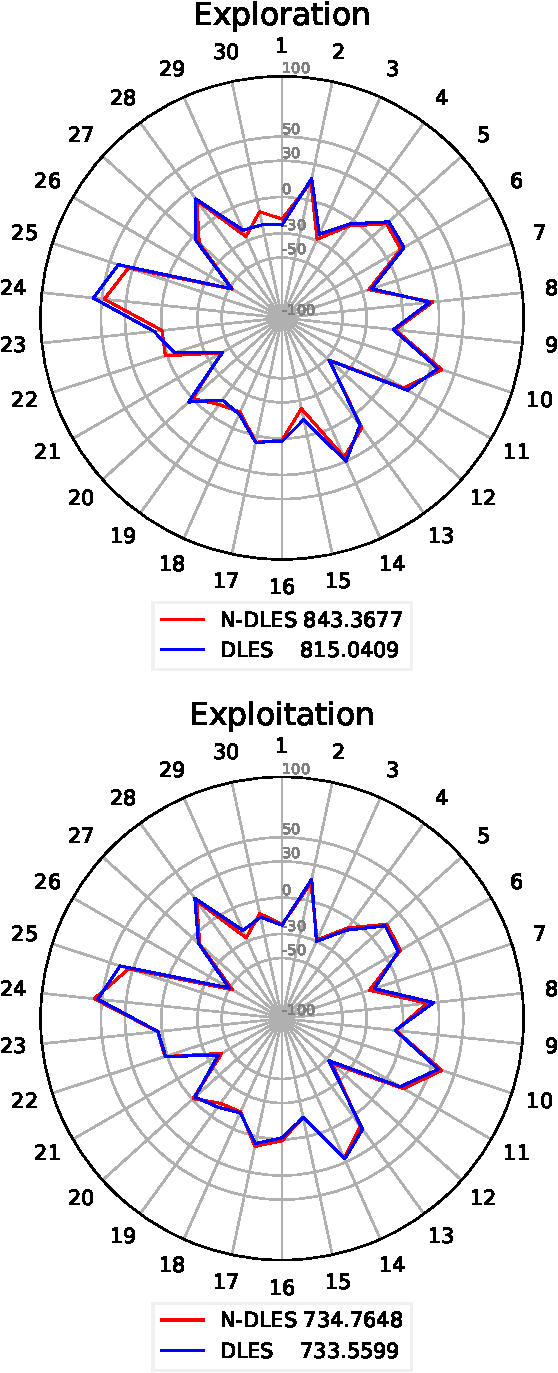
\includegraphics[width=0.8\linewidth]{./renda_1_b.pdf}
		}
	\end{minipage}
	\begin{minipage}[b]{0.3\linewidth}
		\centering
		\subfigure[F12]{
			\label{renda_2}
			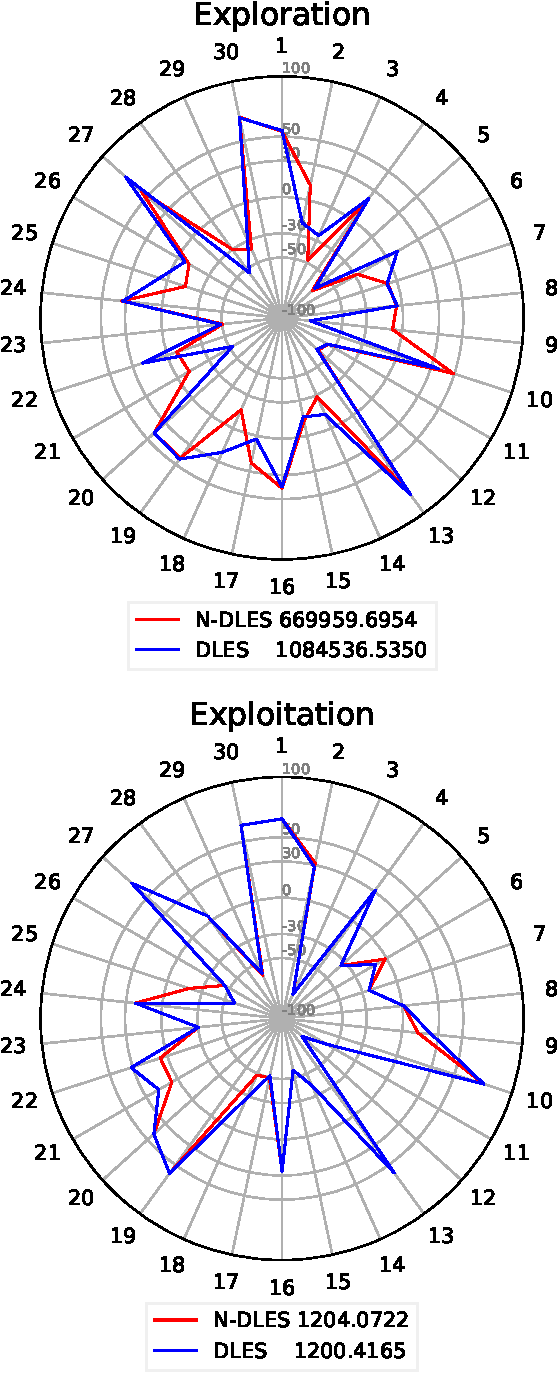
\includegraphics[width=0.8\linewidth]{./renda_2_b.pdf}
		}
	\end{minipage}
	\begin{minipage}[b]{0.3\linewidth}
		\centering
		\subfigure[F29]{
			\label{renda_3}
			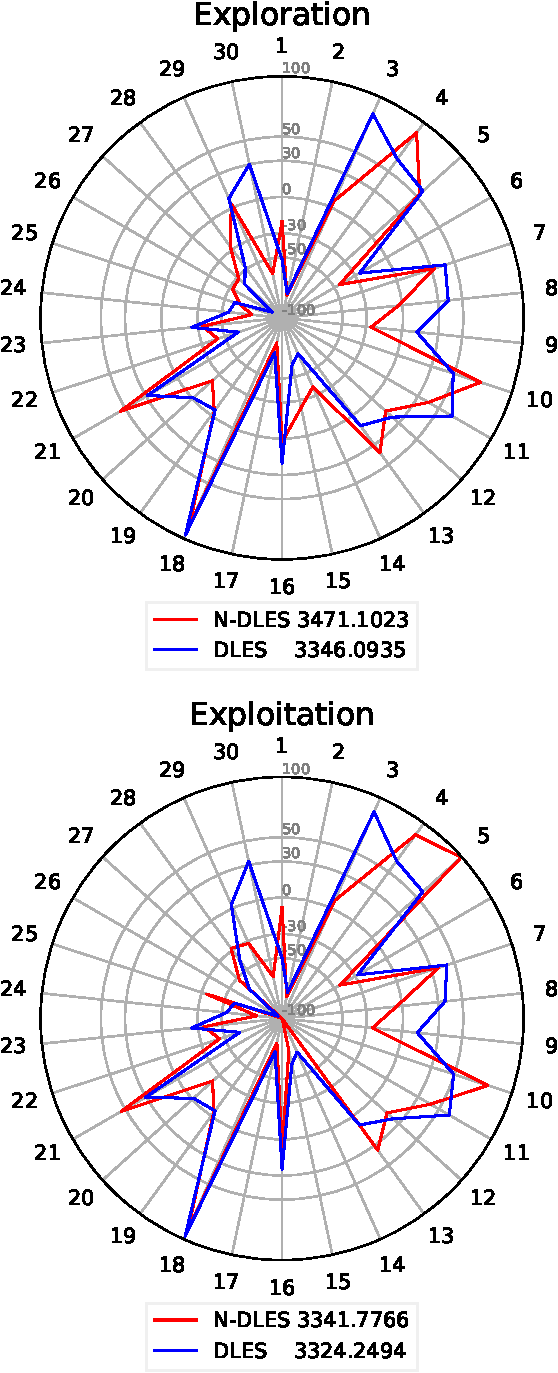
\includegraphics[width=0.8\linewidth]{./renda_3_b.pdf}
		}
	\end{minipage}
	\vspace{-1mm}
	\caption{Comparative analysis of exploration and exploitation degrees facilitated by network on functions F7, F12, and F29.}
	\label{ee}
	\vspace{-5mm}
\end{figure*}

\section{Network Effectiveness Analysis} \label{net-a}
To provide a more intuitive demonstration of the network's role throughout the entire algorithm, we illustrate radar charts depicting the shapes of individuals in the search space for $D = 30$, showcasing both the exploration and exploitation processes. In the first phase, we conducted exploratory experiments and documented the findings. Subsequently, we employ a neural network to learn from the experimental data, yielding results indicative of the network's reconstruction. Simultaneously, we also compared the final exploitation outcomes of two corresponding solutions that underwent a similar process. For a more intuitive representation of the network's influence, we selected three representative experimental plots, F7, F12, and F29, presented in Fig.~\ref{ee}. The exploratory results are displayed on the left side of Fig.~\ref{ee}, while the right side showcases the final development outcomes after the same development operations. The red line represents the results obtained through network reconstruction (DLES), while the blue line represents results without network (N-DLES). The labels in the bottom-left corner annotate the method along with its corresponding fitness values. By contrasting these two lines, we can clearly observe the influence of network reconstruction on experimental outcomes and the differences in the final development results for various solutions.

In the first scenario, as seen in Fig.~\ref{ee}(a), after network reconstruction, no superior result is identified, and the shapes of the two solutions in the solution space remain largely consistent. Consequently, when these solutions undergo the same process, their final outcomes align closely. In the second scenario, as illustrated in Fig.~\ref{ee}(b), there exists a notable disparity between the solutions provided by the network and the algorithmic solutions. Despite the network's solutions having higher fitness values during the exploration phase, the individuals provided by the network outperform the algorithmic solutions in the quality of the final solution during the process. In the third scenario, as illustrated in Fig.~\ref{ee}(c), the exploration results obtained after network reconstruction exhibit significant differences from the algorithmic results. It is evident that the exploration results provided by the network have lower fitness values compared to the algorithm. Simultaneously, from the perspective of final outcomes, the exploration results provided by the network demonstrate a superior exploitation effect. 

This comparison underscores that the network evaluates the superiority of explored individuals not solely based on fitness but rather comprehensively, taking into account the information gleaned from the fitted solution space.

\begin{figure}
	\centering
	\subfigure[$D=30$]{
		\begin{minipage}[b]{0.3\textwidth}
			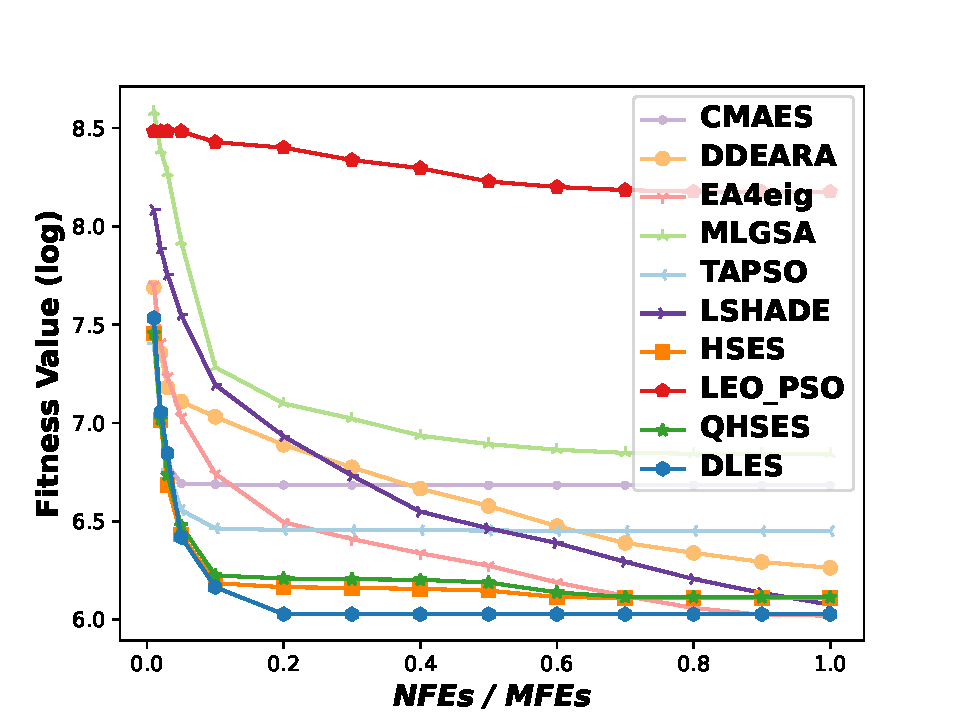
\includegraphics[width=\linewidth]{./F29_D30_L.pdf} 
			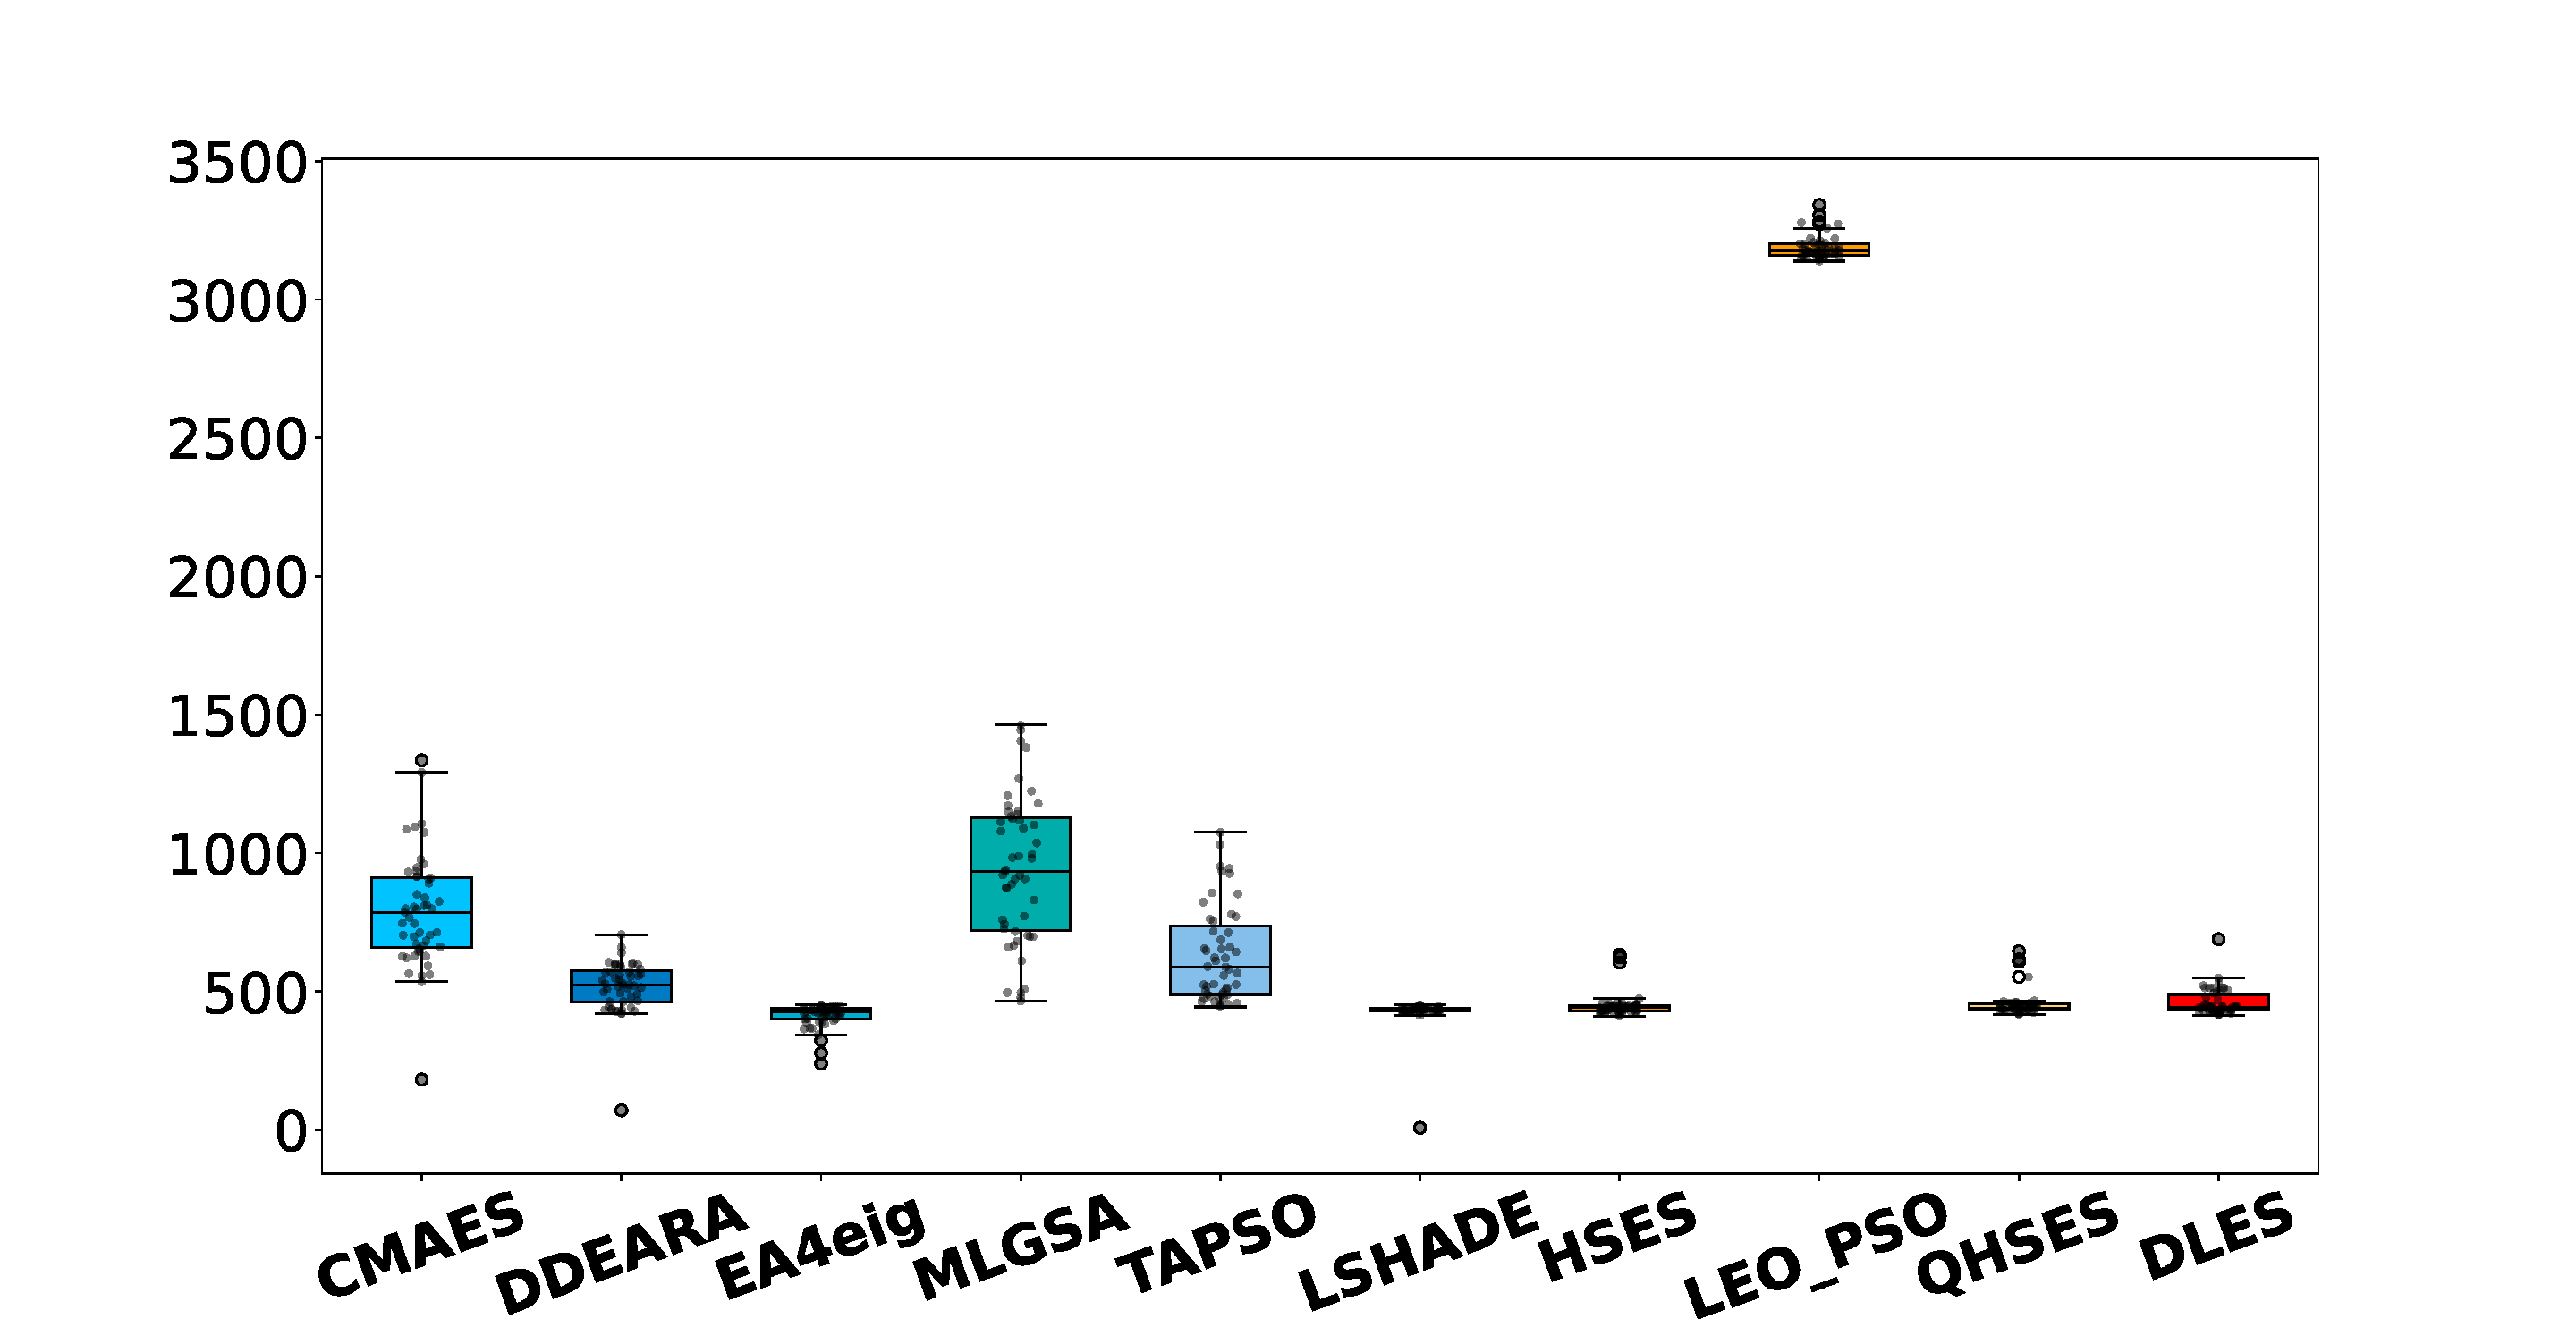
\includegraphics[width=\linewidth]{./F29_D30_B.pdf} 
		\end{minipage}
		\label{fig:grid_4figs_1cap_4subcap_1}
	}
	\subfigure[$D=50$]{
		\begin{minipage}[b]{0.3\textwidth}
			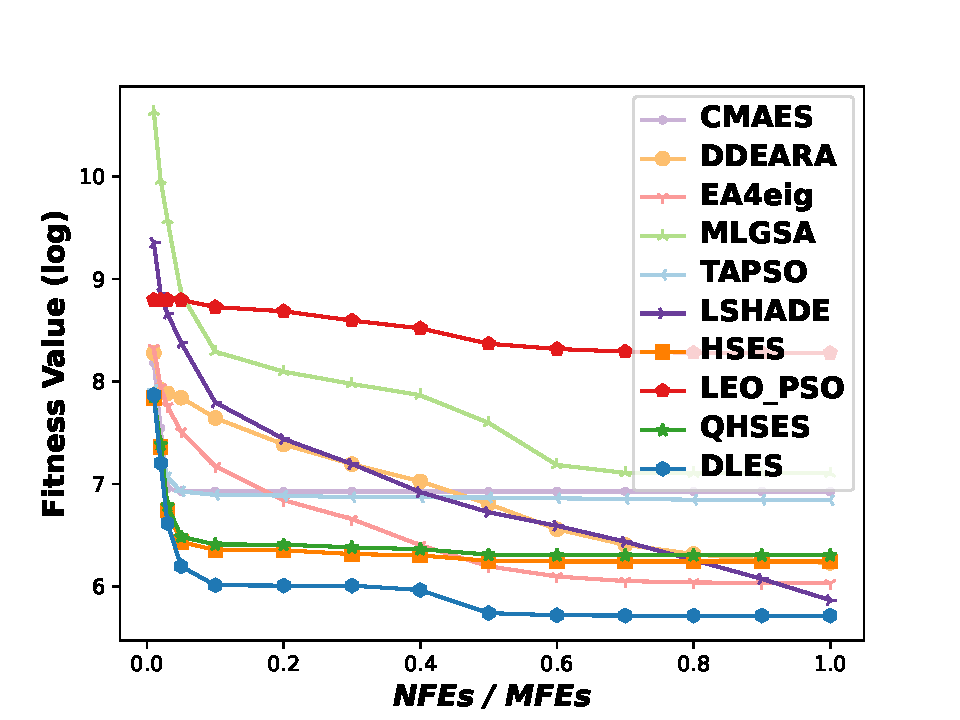
\includegraphics[width=\linewidth]{./F29_D50_L.pdf} 
			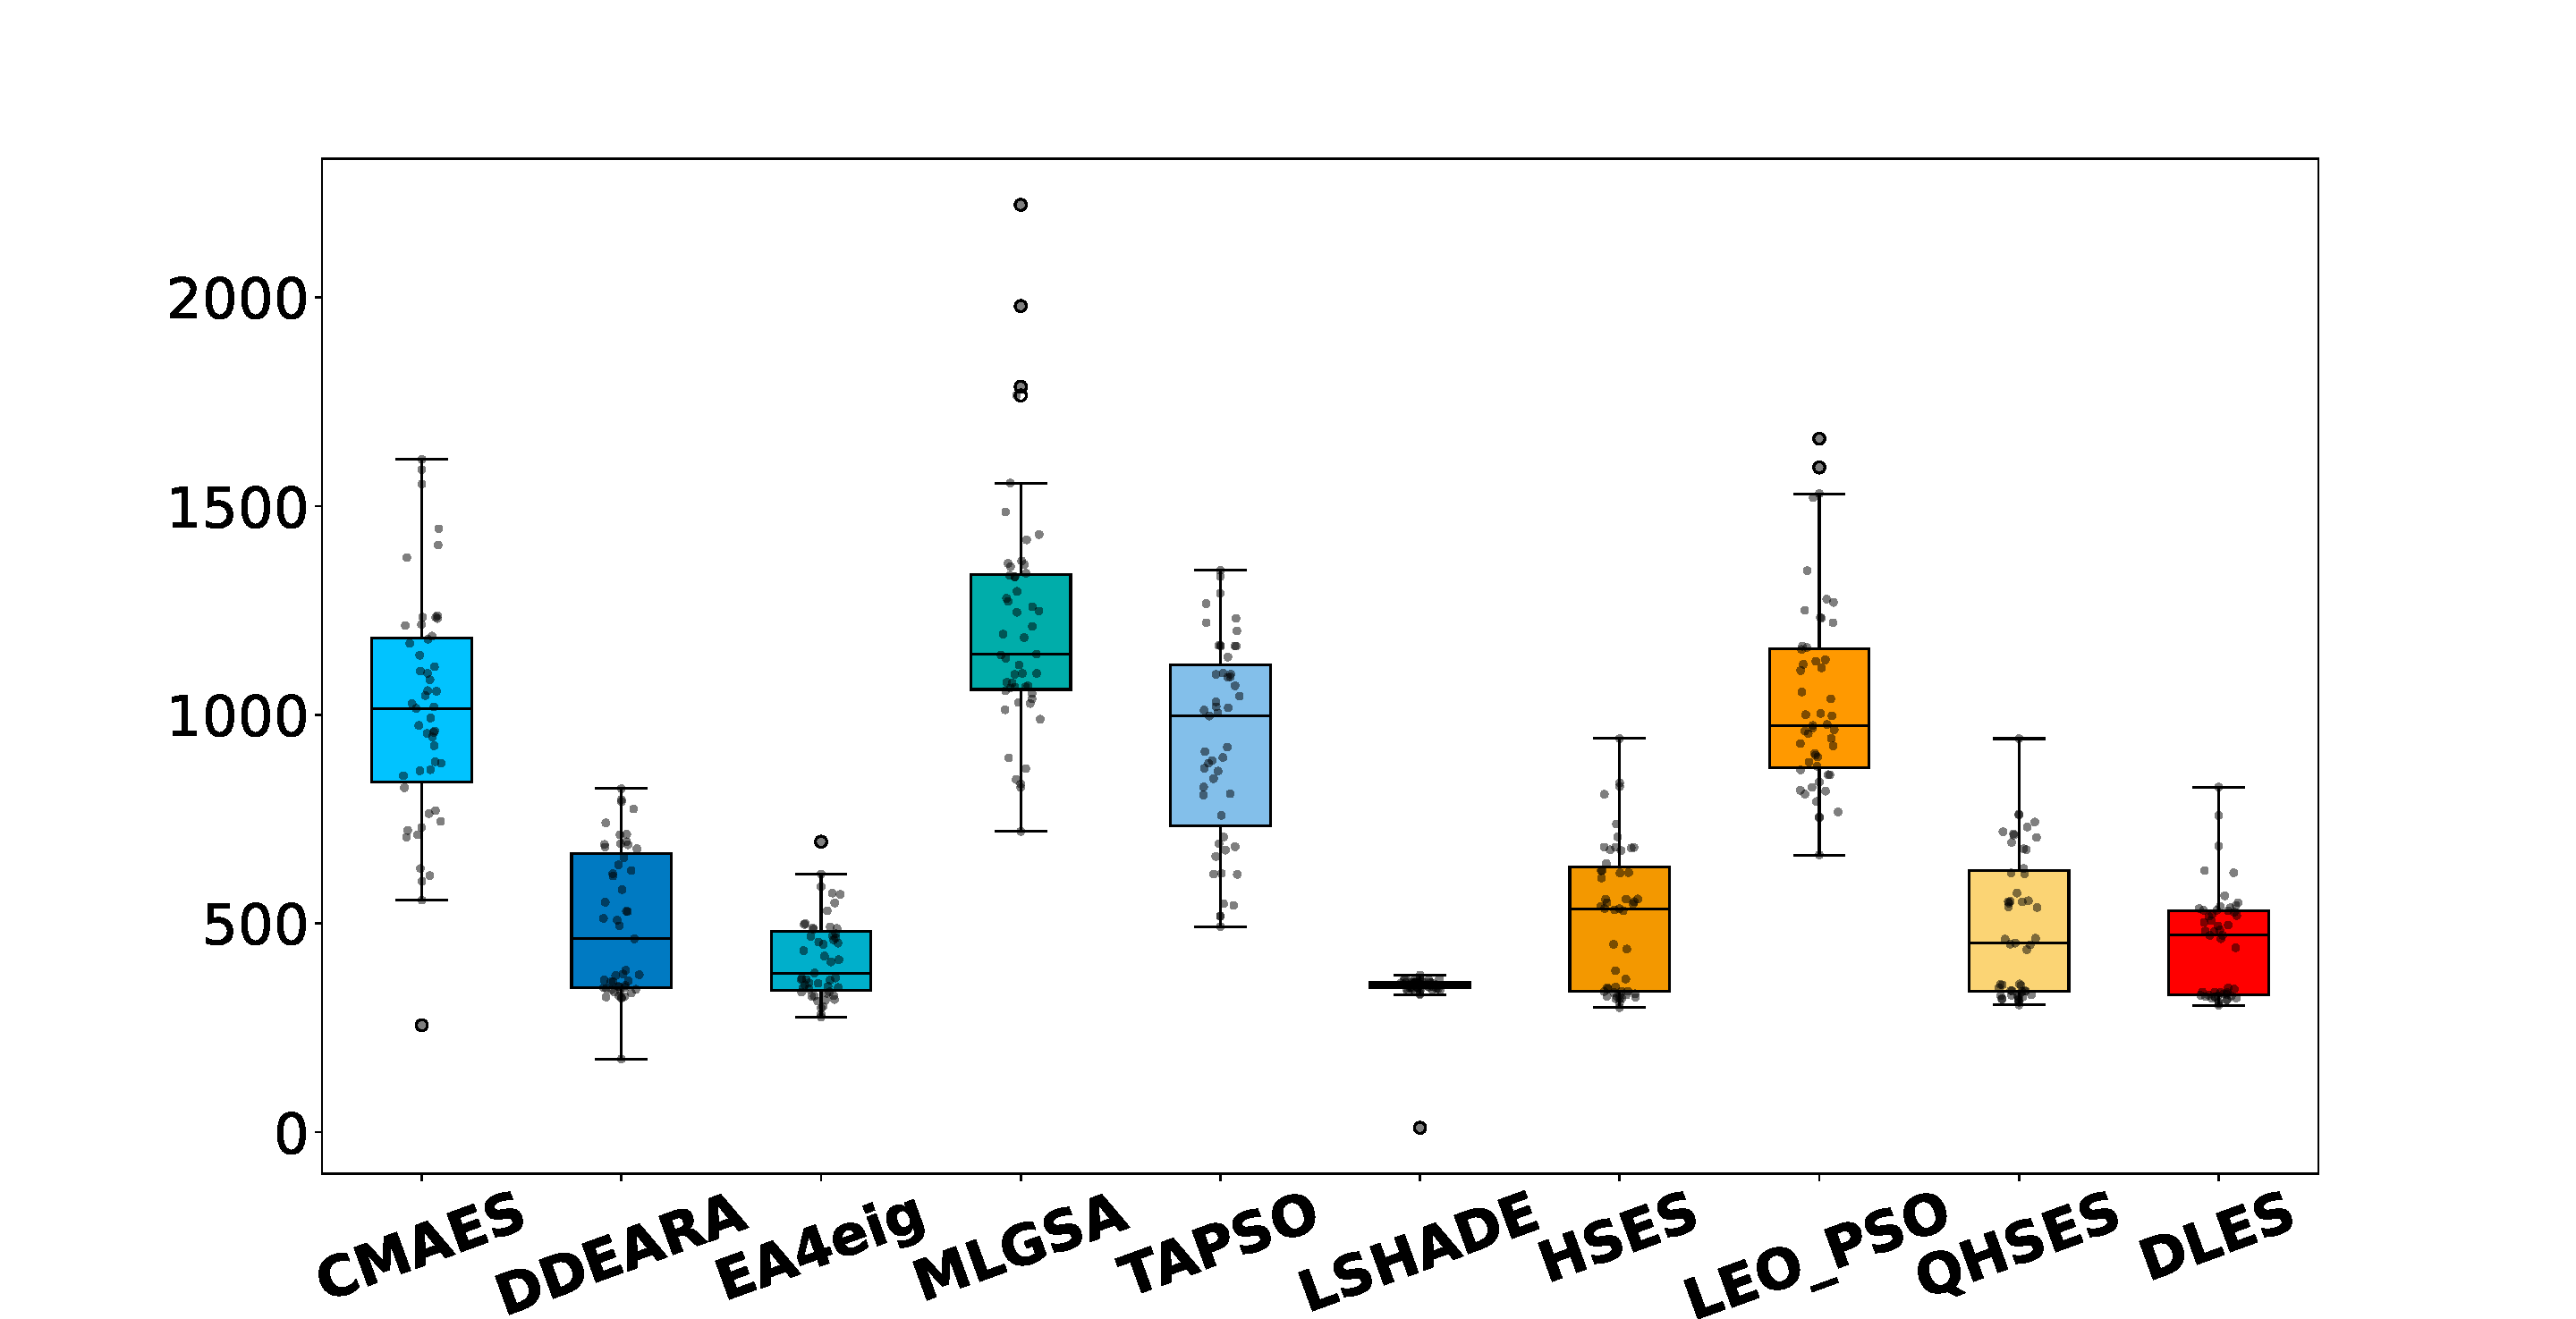
\includegraphics[width=\linewidth]{./F29_D50_B.pdf} 
		\end{minipage}
		\label{fig:grid_4figs_1cap_4subc3ap_1}
	}
	\subfigure[$D=100$]{
		\begin{minipage}[b]{0.3\textwidth}
			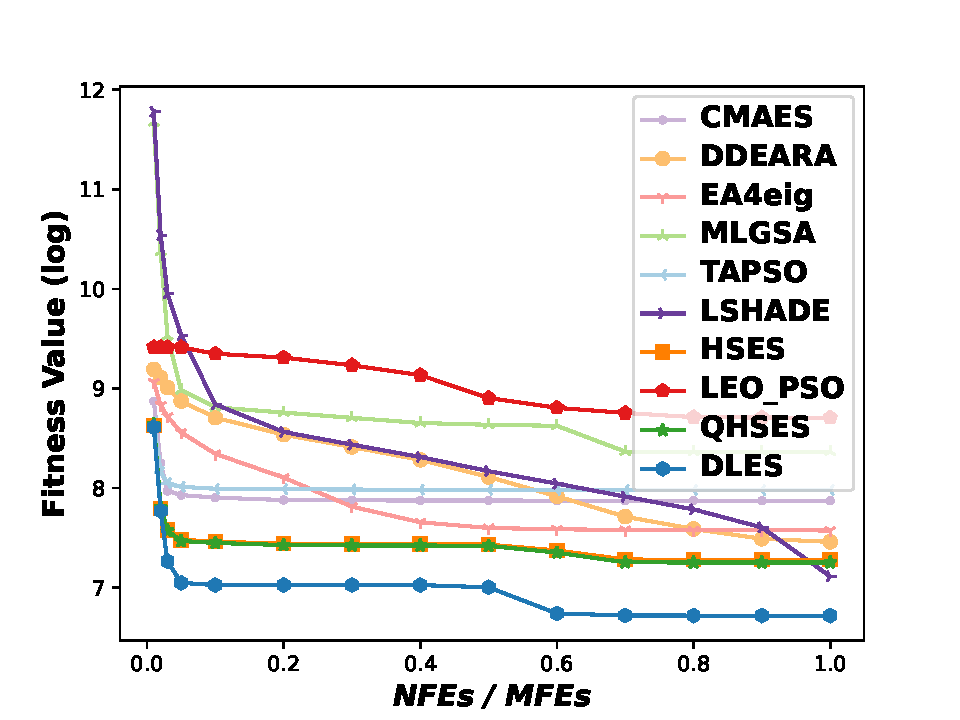
\includegraphics[width=\linewidth]{./F29_D100_L.pdf} 
			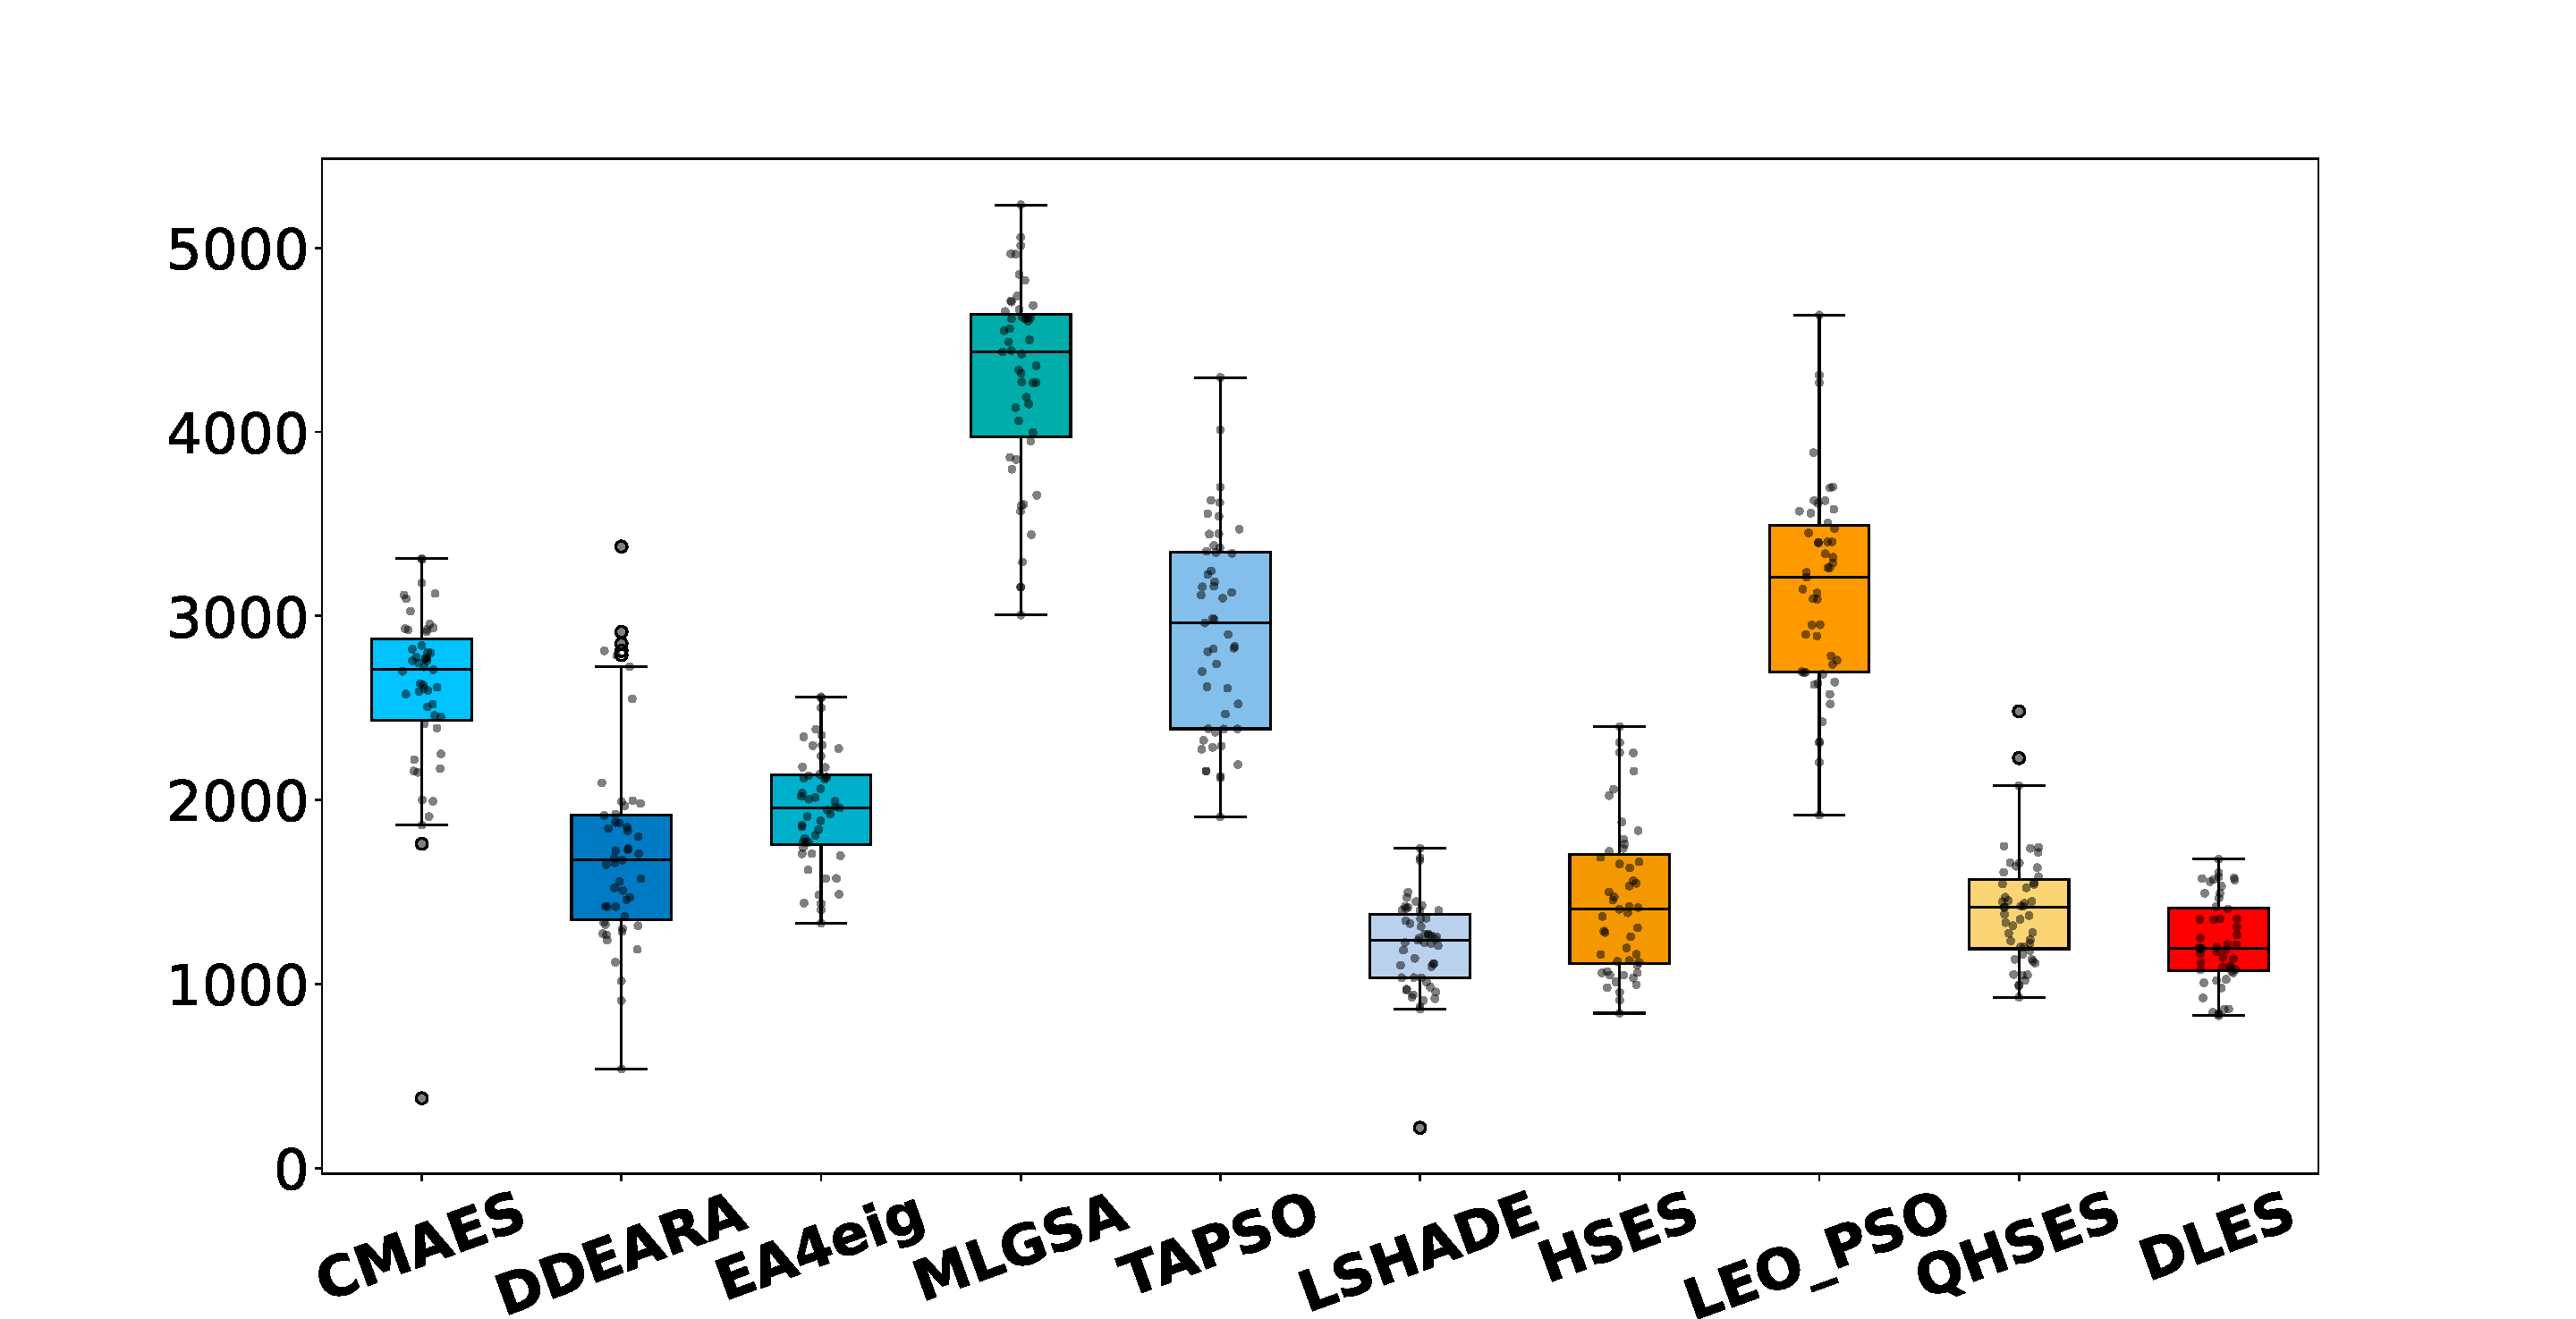
\includegraphics[width=\linewidth]{./F29_D100_B.pdf} 
		\end{minipage}
		\label{fig:grid_4figs_1cap_4subcap23_1}
	}\vspace{-2mm}
	\caption{Optimization curves and Box whisker plots of DLES and other competitors on F29 in CEC 2018 test suite, (a) $D$=30, (b) $D$=50, and (c) $D$=100.}
	\label{f29ind}
\end{figure}

As shown in Fig.~\ref{f29ind}, to better illustrate the outstanding performance of DLES in addressing high-dimensional problems, we select the mixed problem F29 from the CEC 2018 for illustration. In dimensions 30, 50, and 100, we plot convergence curves and box whisker plots to showcase the performance of DLES across various dimensions comprehensively. Within the $M\!F\!E\!s$, we selected 14 data points in accordance with the specified proportion by the official CEC 2018 guidelines. The ordinate, for enhanced observation, is presented using the logarithmic values of fitness. This representation method offers a clearer depiction of the variation trends in algorithm fitness curves. Through the examination of average convergence curves from multiple independent repeated experiments, it becomes evident that DLES exhibits faster convergence rates and superior final convergence results when addressing high-dimensional problems.

In the corresponding box whisker plots, where the abscissa denotes the compared algorithms and the ordinate represents the final convergence fitness across 51 independent repeated experiments. It is discernible that the stability of DLES in multiple independent repeated experiments significantly surpasses that of other comparative algorithms. This indicates that DLES not only demonstrates outstanding performance in solving high-dimensional problems but also exhibits high stability, enabling it to better handle challenges.

\begin{table}[h]
	\centering
	\caption{\textcolor{blue}{Classification of CEC 2014, 2018, 2022 problems by type.}}
	\vspace{-2mm}
	\label{cec_f_c}
	\color{blue}
	%\phantom{0}
	\resizebox{\linewidth}{!}{
		\begin{tabular}{c|ccc|c}	
			\hline							
			Problem categories  & CEC 2014 &	CEC 2018	& CEC 2022	& Number of Problems \\
			\hline		
			Unimodal functions &  F1-F3 & F1-F2 & F1 & 6 \\
			Simlpe multimodal functions &  F4-F16 & F3-F9 & F2-F5 & 24\\
			Hybrid functions & F17-F22 & F10-F19 & F6-F8 & 19\\
			Composition functions &  F23-F30 & F20-F29 & F9-F12 & 22\\
			\hline	
		\end{tabular}
		\vspace{-2mm}
	}
\end{table}

\section{Problem types Analysis}\label{p-a}
To better demonstrate the performance of DLES on various types of problems, we categorize the 71 problems from the CEC series according to the official classification guidelines. The detailed categorization is shown in Table \ref{cec_f_c}. The table shows the classification of CEC 2014, 2018, and 2022 problems. The problems are categorized into four types: Unimodal functions, Simple multimodal functions, Hybrid functions, and Composition functions. The table lists the specific problem indices and the total number for each category. For instance, the Unimodal functions category includes CEC 2014 (F1-F3), CEC 2018 (F1-F2), and CEC 2022 (F1), totaling 6 problems. The classification details for the other categories are similarly provided.

Table \ref{cec-frideall} presents the Friedman rank-sum test scores of DLES and other competing algorithms on the CEC benchmark problems. The evaluation covers various dimensions (10, 20, 30, 50, 100) across four.

In Unimodal functions, DLES consistently performs well across all dimensions, achieving notably low rank-sum scores. This superior performance compared to other algorithms indicates that DLES excels in Unimodal optimization problems, making it one of the top-performing algorithms in this category. For Simple multimodal functions, DLES maintains strong performance across all dimensions, with particularly notable results at $D=10$ and $D=30$, scoring 2.9792 and 2.6667, respectively, which indicates optimal or near-optimal performance. This demonstrates DLES effectiveness in handling the complexity of multimodal problems. In Hybrid functions, DLES’s performance varies: it shows moderate results in lower dimensions (e.g., $D=10$ and $D=20$) but significantly improves in higher dimensions ($D=30, 50, 100$). For instance, at $D=50$ and $D=100$, DLES scores 1.8947 and 1.8421, respectively, outperforming most competing algorithms and highlighting its adaptability to high-dimensional hybrid problems. In Composition functions, DLES exhibits stable performance, suggesting near-optimal or upper-tier performance. It performs exceptionally well in medium to high dimensions, with its best results at $D=100$, where it scores 2.8864. This underscores DLES's significant advantage in handling complex composition problems and high-dimensional search spaces.

Overall, DLES demonstrates outstanding performance on Unimodal and Simple multimodal functions, maintaining superior results across all dimensions. In hybrid and composition functions, DLES shows strong performance in higher dimensions, though with some variability in lower dimensions. Therefore, DLES is particularly well-suited for Unimodal and Simple multimodal optimization problems and also performs competitively in high-dimensional Hybrid and Composition problems.

\begin{table}[h]
	\centering
	\caption{\textcolor{blue}{Friedman rank-sum test scores of DLES and other competitors on cec bechmarks}}
	\vspace{-2mm}
	\label{cec-frideall}
	\color{blue}
	%\phantom{0}
	\resizebox{\linewidth}{!}{
		\begin{tabular}{l|c|ccc|ccccccc}	
			\hline							
			& Dimension & DLES  &	LEO-PSO	&	QHSES	&	CMAES	&	DDEARA	&	EA4eig	&	HSES	&	LSHADE	&	TAPSO	&	MLGSA \\
			\hline															
			\multirow{5}{*}{Unimodal Functions}	
			& $D$ =  10  &  \textbf{3.7500} & 8.0833 & \textbf{3.7500} &\textbf{3.7500} & 6.6667 & 4.8333 & 4.3333 & 3.7500 & 7.7500 & 8.3333 \\
			& $D$ =  20  &  \textbf{3.5000} & \textbf{3.5000} & \textbf{3.5000} & \textbf{3.5000} & \textbf{3.5000} & 10.0000 & 8.0000 & 3.5000 & 9.0000 & 7.0000 \\
			& $D$ =  30  &  \textbf{2.9167} & 7.5000 & \textbf{2.9167} & \textbf{2.9167} & 7.5000 & 3.4167 & \textbf{2.9167} & \textbf{2.9167} & 5.8333 & 7.0000 \\
			& $D$ =  50  &  \textbf{2.3333} & 6.5000 & 2.7500 & \textbf{2.3333} & 7.3333 & 3.2500 & 3.1667 & 3.8333 & 6.8333 & 7.5000 \\
			& $D$ =  100  &  \textbf{1.8333} & 6.3333 & 2.0833 & 1.8333 & 7.3333 & 5.0000 & 3.2500 & 3.8333 & 6.6667 & 7.6667 \\
			\hline																							
			\multirow{5}{*}{Simple multimodal functions}	
			& $D$ =  10  &  \textbf{2.9792} & 7.3125 & 4.1042 & 8.8958 & 7.0833 & 4.2500 & 3.7292 & 3.3125 & 6.5833 & 6.7500 \\
			& $D$ =  20  &  \textbf{3.1250} & 3.8750 & 3.6250 & 7.2500 & 3.6250 & 10.0000 & 4.5000 & 4.2500 & 8.7500 & 6.0000 \\
			& $D$ =  30  &  \textbf{2.6667} & 4.5833 & 3.2083 & 7.2500 & 6.9583 & 3.9167 & 3.1667 & 2.7500 & 5.7500 & 5.5833 \\
			& $D$ =  50  &  \textbf{2.1667} & 4.5833 & 2.9167 & 7.0833 & 7.2917 & 4.3958 & 2.8542 & 3.6458 & 5.4375 & 5.4583 \\
			& $D$ =  100  &  \textbf{2.3542} & 4.0417 & 2.9792 & 6.6667 & 7.2708 & 4.5625 & 2.6875 & 4.0833 & 5.6458 & 5.5417 \\
			\hline																							
			\multirow{5}{*}{Hybrid Functions}	
			& $D$ =  10  &  4.3684 & 8.3158 & 4.6842 & 8.4211 & 3.8421 & \textbf{2.7105} & 4.5263 & 2.2895 & 8.3158 & 7.5263 \\
			& $D$ =  20  &  5.3333 & 5.3333 & 3.0000 & 7.3333 & 3.3333 & 9.6667 & 4.3333 & \textbf{1.0000} & 9.3333 & 6.3333 \\
			& $D$ =  30  &  2.6842 & 6.5789 & 2.8947 & 6.1579 & 5.5789 & 2.6316 & \textbf{2.5263} & 2.8947 & 7.1053 & 7.2632 \\
			& $D$ =  50  &  \textbf{1.8947} & 6.0000 & 2.4211 & 6.0000 & 6.5789 & 4.1579 & 1.9474 & 3.1579 & 6.8947 & 7.2632 \\
			& $D$ =  100  &  \textbf{1.8421} & 5.8421 & 2.3684 & 5.3158 & 6.8421 & 4.4211 & 2.2105 & 3.7895 & 6.4737 & 7.2105 \\
			\hline	
			
			\multirow{5}{*}{Composition Functions}	
			& $D$ =  10  &  5.5000 & 6.4545 & 5.5227 & 8.2045 & 3.6136 & \textbf{2.0909} & 6.0909 & 4.1136 & 6.7727 & 6.6364 \\
			& $D$ =  20  &  3.5000 & 4.2500 & 6.0000 & 8.0000 & 3.0000 & \textbf{1.0000} & 5.5000 & 7.7500 & 9.7500 & 6.2500 \\
			& $D$ =  30  &  3.0000 & 5.4545 & 3.7727 & 6.4545 & 5.8864 & \textbf{2.9545} & 3.5227 & 3.0000 & 6.3636 & 4.5909 \\
			& $D$ =  50  &  3.5455 & 5.0455 & 3.5000 & 5.8182 & 6.2727 & \textbf{2.5909} & 3.4545 & 3.4773 & 5.8864 & 5.4091 \\
			& $D$ =  100  &  \textbf{2.8864} & 5.0000 & 3.0000 & 5.4091 & 6.3636 & 3.8636 & 3.0455 & 3.7273 & 6.2273 & 5.4773 \\
			\hline																						\end{tabular}
		\vspace{-2mm}
	}
\end{table}

To provide a more detailed view of DLES performance, we created the Table \ref{cec-Wilcoxon}. This table presents the Wilcoxon rank-sum test results of DLES compared to other algorithms on CEC benchmarks, showing the performance of DLES across different dimensions and problem types in terms of W/T/L (Win/Tie/Loss). Unlike the Friedman rank-sum test table, the Wilcoxon table offers a more granular look at the number of wins and losses for DLES against each competitor, thereby providing a clearer reflection of DLES's relative strengths in specific dimensions and problem types.

\begin{table}[h]
	\centering
	\caption{\textcolor{blue}{Wilcoxon rank-sum test results of DLES and other competitors on cec bechmarks in  different dimensions in terms of W/T/L.}}
	\vspace{-2mm}
	\label{cec-Wilcoxon}
	\color{blue}
	%\phantom{0}
	\resizebox{\linewidth}{!}{
		\begin{tabular}{l|c|ccc|cccccc|c}	
			\hline							
			DLES vs. & Dimension &	LEO-PSO	&	QHSES	&	CMAES	&	DDEARA	&	EA4eig	&	HSES	&	LSHADE	&	TAPSO	&	MLGSA	 &	Total \\
			\hline															
			\multirow{5}{*}{Unimodal Functions}	
			& $D$ = 10 	& 5 / 1 / 0
			& 0 / 6 / 0
			& 0 / 6 / 0
			& 3 / 3 / 0
			& 1 / 5 / 0
			& 1 / 5 / 0
			& 0 / 6 / 0
			& 5 / 1 / 0
			& 6 / 0 / 0
			& 21 / 33 / 0 \\
			& $D$ = 20 	& 0 / 1 / 0
			& 0 / 1 / 0
			& 0 / 1 / 0
			& 0 / 1 / 0
			& 1 / 0 / 0
			& 1 / 0 / 0
			& 0 / 1 / 0
			& 1 / 0 / 0
			& 1 / 0 / 0
			& 4 / 5 / 0 \\
			& $D$ = 30 & 5 / 1 / 0
			& 0 / 6 / 0
			& 0 / 6 / 0
			& 6 / 0 / 0
			& 1 / 5 / 0
			& 0 / 6 / 0
			& 0 / 6 / 0
			& 5 / 1 / 0
			& 5 / 1 / 0
			& 22 / 32 / 0 \\
			& $D$ = 50 & 5 / 1 / 0
			& 1 / 5 / 0
			& 0 / 6 / 0
			& 6 / 0 / 0
			& 1 / 5 / 0
			& 0 / 6 / 0
			& 3 / 3 / 0
			& 6 / 0 / 0
			& 6 / 0 / 0
			& 28 / 26 / 0 \\
			& $D$ = 100 & 5 / 1 / 0
			& 1 / 5 / 0
			& 0 / 6 / 0
			& 6 / 0 / 0
			& 6 / 0 / 0
			& 1 / 5 / 0
			& 5 / 1 / 0
			& 6 / 0 / 0
			& 6 / 0 / 0
			& 36 / 18 / 0 \\
			\hline																							
			\multirow{5}{*}{Simple multimodal Functions}	
			& $D$ = 10  & 20 / 3 / 1
			& 10 / 12 / 2
			& 23 / 1 / 0
			& 18 / 4 / 2
			& 14 / 6 / 4
			& 10 / 12 / 2
			& 12 / 9 / 3
			& 18 / 5 / 1
			& 22 / 1 / 1
			& 147 / 53 / 16 \\
			
			& $D$ = 20 & 1 / 2 / 1
			& 0 / 4 / 0
			& 3 / 1 / 0
			& 1 / 3 / 0
			& 4 / 0 / 0
			& 1 / 2 / 1
			& 2 / 1 / 1
			& 4 / 0 / 0
			& 3 / 1 / 0
			& 19 / 14 / 3 \\
			& $D$ = 30 & 15 / 0 / 5
			& 10 / 6 / 4
			& 17 / 2 / 1
			& 17 / 2 / 1
			& 13 / 2 / 5
			& 8 / 9 / 3
			& 7 / 8 / 5
			& 17 / 0 / 3
			& 16 / 3 / 1
			& 120 / 32 / 28 \\
			& $D$ = 50 & 17 / 0 / 3
			& 10 / 5 / 5
			& 16 / 3 / 1
			& 18 / 0 / 2
			& 15 / 3 / 2
			& 6 / 9 / 5
			& 15 / 2 / 3
			& 18 / 0 / 2
			& 17 / 2 / 1
			& 132 / 24 / 24 \\
			& $D$ = 100 & 13 / 2 / 5
			& 8 / 10 / 2
			& 17 / 2 / 1
			& 17 / 3 / 0
			& 16 / 2 / 2
			& 7 / 9 / 4
			& 16 / 2 / 2
			& 17 / 1 / 2
			& 16 / 3 / 1
			& 127 / 34 / 19 \\
			\hline																							
			\multirow{5}{*}{Hybrid Functions}	
			& $D$ = 10   & 16 / 1 / 2
			& 7 / 7 / 5
			& 18 / 1 / 0
			& 5 / 3 / 11
			& 5 / 1 / 13
			& 6 / 9 / 4
			& 3 / 4 / 12
			& 17 / 0 / 2
			& 16 / 1 / 2
			& 93 / 27 / 51 \\
			& 	$D$ = 20 & 1 / 0 / 2
			& 1 / 0 / 2
			& 3 / 0 / 0
			& 1 / 1 / 1
			& 3 / 0 / 0
			& 0 / 3 / 0
			& 0 / 0 / 3
			& 3 / 0 / 0
			& 2 / 1 / 0
			& 14 / 5 / 8 \\
			& $D$ = 30 & 14 / 0 / 2
			& 6 / 7 / 3
			& 16 / 0 / 0
			& 12 / 2 / 2
			& 10 / 3 / 3
			& 4 / 10 / 2
			& 9 / 2 / 5
			& 15 / 0 / 1
			& 16 / 0 / 0
			& 102 / 24 / 18 \\
			& $D$ = 50 & 14 / 1 / 1
			& 7 / 5 / 4
			& 16 / 0 / 0
			& 16 / 0 / 0
			& 16 / 0 / 0
			& 6 / 6 / 4
			& 13 / 2 / 1
			& 16 / 0 / 0
			& 16 / 0 / 0
			& 120 / 14 / 10 \\
			& $D$ = 100 & 12 / 2 / 2
			& 5 / 10 / 1
			& 14 / 1 / 1
			& 14 / 1 / 1
			& 13 / 1 / 2
			& 6 / 8 / 2
			& 14 / 1 / 1
			& 14 / 1 / 1
			& 14 / 1 / 1
			& 106 / 26 / 12 \\
			\hline	
			
			\multirow{5}{*}{Composition Functions}	
			& 	$D$ = 10 	& 11 / 5 / 6
			& 11 / 5 / 6
			& 16 / 2 / 4
			& 6 / 2 / 14
			& 5 / 4 / 13
			& 12 / 6 / 4
			& 7 / 5 / 10
			& 16 / 1 / 5
			& 15 / 2 / 5
			& 99 / 32 / 67 \\
			& $D$ = 20 & 1 / 0 / 3
			& 3 / 0 / 1
			& 3 / 1 / 0
			& 1 / 1 / 2
			& 0 / 0 / 4
			& 2 / 2 / 0
			& 3 / 0 / 1
			& 4 / 0 / 0
			& 3 / 1 / 0
			& 20 / 5 / 11 \\
			& $D$ = 30 & 12 / 1 / 5
			& 9 / 4 / 5
			& 13 / 0 / 5
			& 14 / 1 / 3
			& 10 / 0 / 8
			& 8 / 6 / 4
			& 8 / 3 / 7
			& 16 / 1 / 1
			& 11 / 1 / 6
			& 101 / 17 / 44 \\
			& $D$ = 50 & 11 / 1 / 6
			& 4 / 9 / 5
			& 11 / 0 / 7
			& 15 / 0 / 3
			& 7 / 1 / 10
			& 5 / 8 / 5
			& 10 / 2 / 6
			& 14 / 1 / 3
			& 13 / 0 / 5
			& 90 / 22 / 50 \\
			& $D$ = 100 & 11 / 1 / 6
			& 5 / 9 / 4
			& 12 / 2 / 4
			& 16 / 1 / 1
			& 10 / 4 / 4
			& 4 / 9 / 5
			& 10 / 4 / 4
			& 15 / 1 / 2
			& 13 / 1 / 4
			& 96 / 32 / 34 \\
			\hline																						\end{tabular}
		\vspace{-2mm}
		}
\end{table}

\begin{table*}[h]
	\centering
	\caption{\textcolor{blue}{Comparison scores of DLES use different network on cec 2018 benchmark.}}
	\vspace{-2mm}
	\label{d-network}
	\color{blue}
	%\phantom{0}
	\resizebox{\linewidth}{!}{
		\begin{tabular}{c|c|cccccc}	
			\hline							
			Dimension	& Functions & No-Net &	Net1  &	Net2	&	Net3	&	Net4	& Net5 \\	
			\hline														
			\multirow{5}{*}{$D$ = 10}	
			& Unimodal Functions &  \textbf{3.5000} &  \textbf{3.5000} & \textbf{3.5000} &  \textbf{3.5000} & \textbf{3.5000} & \textbf{3.5000} \\
			& Simple multimodal Functions & 4.3571 & 3.2143 & 3.9286 & 3.2143 & 3.5000 & \textbf{	2.7857} \\
			& Hybrid Functions 	& 3.6000 & 3.3000 & \textbf{2.7000} & 4.4500 & 2.7500 & 4.2000 \\
			& Composition Functions & 4.5000 & 3.0000 & 3.6000 & \textbf{2.7000} & 3.7000 & 3.5000 \\
			& All Functions & 4.0862 & \textbf{3.1897} & 3.3621 & 3.4828 & 3.3103 & 3.5690 \\
			\hline
			
			\multirow{5}{*}{$D$ = 30}	
			& Unimodal Functions & \textbf{3.5000} &  \textbf{3.5000} &  \textbf{3.5000}&  \textbf{3.5000} &  \textbf{3.5000} &  \textbf{3.5000}\\
			& Simple multimodal Functions & 3.4286 & 3.5714 & 4.2857 & \textbf{2.5714} & 3.0000 & 4.1429 \\
			& Hybrid Functions  & \textbf{2.5000} & 4.9000 & 5.0000 & 3.1000 & 2.9000 & 2.6000 \\
			& Composition Functions & 4.2000 & 3.8000 & 3.3000 & \textbf{3.1500} & 3.2500 & 3.3000 \\
			& All Functions & 3.3793 & 4.1034 & 4.1379 & \textbf{3.0172} & 3.0862 & 3.2759 \\
			\hline
			
			\multirow{5}{*}{$D$ = 50}	
			& Unimodal Functions & \textbf{1.5000} &  3.5000 &  5.5000 &  3.7500 &  4.0000 &  2.7500 \\
			& Simple multimodal Functions & \textbf{2.5714} & 4.2857 & 4.8571 & 3.7143 & 3.0000 & 2.5714 \\
			& Hybrid Functions & 3.9000 & 4.2000 & 3.8000 & \textbf{2.7000} & 3.1000 & 3.3000 \\
			& Composition Functions & 3.4000 & 4.0000 & \textbf{2.9000} & 3.8000 & 3.5000 & 3.4000 \\
			& All Functions & 3.2414 & 4.1034 & 3.8621 & 3.3966 & 3.2759 & \textbf{3.1207} \\
			\hline	
			
			\multirow{5}{*}{$D$ = 100}	
			& Unimodal Functions & \textbf{3.2500} &  \textbf{3.2500} &  \textbf{3.2500} &  \textbf{3.2500} &  \textbf{3.2500} &  4.7500 \\
			& Simple multimodal Functions& \textbf{3.0000} & 4.1429 & 3.4286 & 3.7857 & \textbf{3.0000} & 3.6429 \\
			& Hybrid Functions & 3.5000 & 3.3000 & 4.3000 & \textbf{2.5000} & 3.9000 & 3.5000 \\
			& Composition Functions & 3.5000 & 3.4000 & 4.1000 & 3.8000 & \textbf{2.7000} & 3.5000 \\
			& All Functions & 3.3621 & 3.5345 & 3.9483 & 3.3103 & \textbf{3.2241} & 3.6207 \\
			\hline
			%\textbf{	}
		\end{tabular}
		\vspace{-2mm}
	}
\end{table*}

\section{Network Structures Analysis}\label{ns-a}
To illustrate the impact of different network depths and widths on algorithm performance, we present Table \ref{d-network}, where ``No-net'' refers to the scenario without network fitting, while ``Net1'' to ``Net5'' represent networks of varying complexities. The specific structures of Net1 to Net5 can be found in Section VI-D, in the main text.

As shown in Table \ref{d-network}, using different network structures generally improves performance compared to ones without using a network. This trend is evident across all problem types and dimensions. This indicates that incorporating network structures enhances DLES's capability to address complex optimization problems.

In $D=10$, networks consistently outperform the No-Net configuration across all problem types. For Simple multimodal functions, Net5 achieves the best score of 2.7857, demonstrating the advantage of a network structure. In Hybrid functions, Net2 performs best with a score of 2.7000, showing notable improvement over the No-Net approach. Similarly, in Composition functions, Net3 shows the best performance with a score of 2.7000. In $D=30$, The trend continues with network structures generally providing better results. For Simple multimodal functions, Net4 has the highest score of 2.5714, reflecting its superior performance in this dimension. Hybrid functions see the best results with Net1 at 2.5000, while Net3 excels in Composition functions with a score of 3.1500. Overall, Net4 and Net3 demonstrate significant advantages across different problem types. In $D=50$, the variation in performance between networks becomes more pronounced. Net3 achieves the best result in Hybrid functions with a score of 2.7000. The overall performance in all functions is highest with Net5 at 3.1207, indicating its effectiveness in handling various problem types at this dimension. In $D=100$, in this dimension, network structures again demonstrate superior performance compared to No-Net. Notably, Net4 excels in Unimodal, Simple multimodal, and Composition functions, achieving an overall score of 3.2241 across all functions. This highlights Net4's robust performance across various problem types.

Using network structures generally leads to better performance. Typically, as the complexity of the problem and the dimensionality increase, more complex networks yield better results. However, for simpler problems, using more complex networks can sometimes lead to a decrease in performance. This may be since, under limited evaluation conditions, training complex networks requires more high-quality training samples and resources, making it challenging to train such networks effectively.

Selecting the most suitable network for different problems is more effective. However, this approach would result in an algorithm tailored to specific problems, which contradicts the objective of our research. Therefore, we choose Net3, which maintains good performance across most scenarios, as our base network.

\textcolor{blue}{
The choice of activation function is also an important aspect worth discussing in the network. In our network, we choose Tanh as the activation function. Table \ref{ac_select} presents the Friedman score rankings for various activation functions on the CEC 2018 test set with $D$ = 30, where Tanh achieves the highest score of 3.7759. Compared to other activation functions, Tanh offers several advantages. First, its output range of [-1, 1] promotes balanced outputs, which helps center the data around zero and accelerates the convergence process. Second, it provides smoother gradient transitions, reducing the likelihood of vanishing gradients that can hinder effective backpropagation in deep networks. Lastly, Tanh is zero-centered, which minimizes bias effects and facilitates faster learning. In contrast, functions like ReLU, while effective in promoting sparse activations, score lower, possibly due to their zero-gradient behavior for negative inputs, which can halt parameter updates. Although Sigmoid shows a score close to Tanh, it is more prone to gradient vanishing issues, which impacts training efficiency. Thus, Tanh is selected for its overall balance of performance and stability.}
\begin{table*}[h]
	\centering
	\caption{\textcolor{blue}{Friedman Score Ranking of Different Activation Functions on CEC 2018 in D=30 }}
	\vspace{-2mm}
	\label{ac_select}
	\color{blue}
	%\phantom{0}
	\resizebox{\linewidth}{!}{
		\begin{tabular}{c|cccccccc}	
			\hline							
			Activation Function	& Tanh & Sigmoid &	Softsign  &	Softmax	&	ReLU	&	LeakyReLU	& PReLU & ReLU6 \\	
			\hline	
			Score &  \textbf{3.7759} & 3.7931 & 4.4483 & 4.1552 & 5.0172 & 5.4828 & 4.9655 & 4.3621 \\
			Rank &	1 &2 &5 &3 &7 &8 &6 & 4 \\
			\hline												
			%\textbf{	}
		\end{tabular}
		\vspace{-2mm}
	}
\end{table*}

\section{The post-hoc test in BBOB}\label{p-b}
The post-hoc test facilitates a deeper understanding of DLES' performance and behavior after initial evaluations. By meticulously examining the results, we can identify underlying patterns, assess the impact of various factors, and uncover potential avenues for enhancement. This process not only validates our findings but also provides a comprehensive view of our models' performance across different conditions, thereby informing future research and development directions. Consequently, we performed a post-hoc analysis on the BBOB dataset.
We use runtime distributions (ECDFs) to illustrate the performance differences between DLES and other competing algorithms. ECDFs plots provide an intuitive visualization of the runtime efficiency across all tested targets, showing how frequently the algorithms solve problems quickly and the typical runtime required to meet specific performance targets. The the overall results presented in Fig. \ref{bbob-over}.

It can be observed that DLES demonstrates superior performance across all compared dimensions. It achieves the best rankings in 2, 3, and 10 dimensional cases and exhibits fast convergence speeds. In 5, 20, and 40 dimensional cases, DLES only slightly underperforms compared to a-CMAES, an advanced variant of CMA-ES, but still outperforms other competing methods, including the original CMA-ES and its variant sc-CMAES. In terms of convergence speed, DLES is also comparable to a-CMAES.


\begin{figure}[H]
	\centering
	\begin{minipage}[b]{0.3\textwidth}
		\centering
		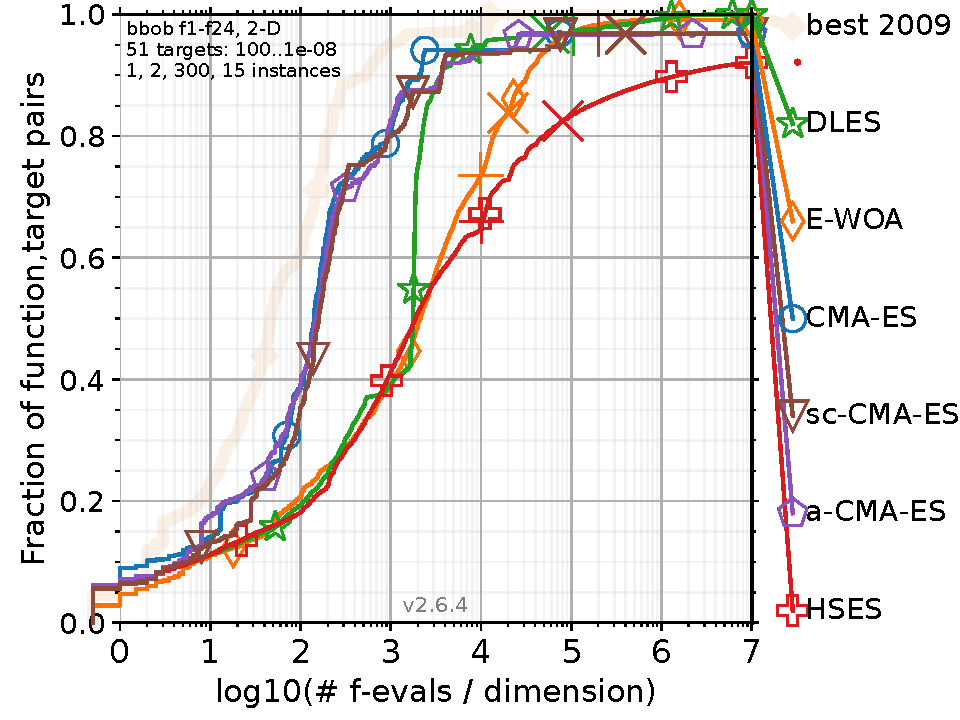
\includegraphics[width=\textwidth]{./bbob/pprldmany_02D_noiselessall.pdf}
	\end{minipage}\hfill
	\begin{minipage}[b]{0.3\textwidth}
		\centering
		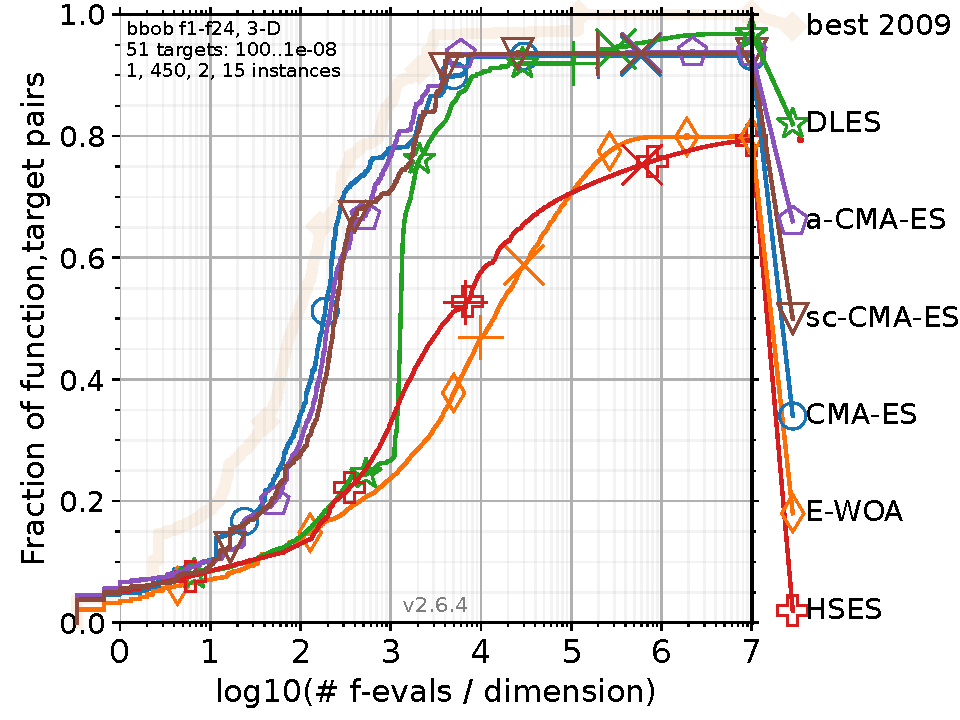
\includegraphics[width=\textwidth]{./bbob/pprldmany_03D_noiselessall.pdf}
	\end{minipage}\hfill
	\begin{minipage}[b]{0.3\textwidth}
		\centering
		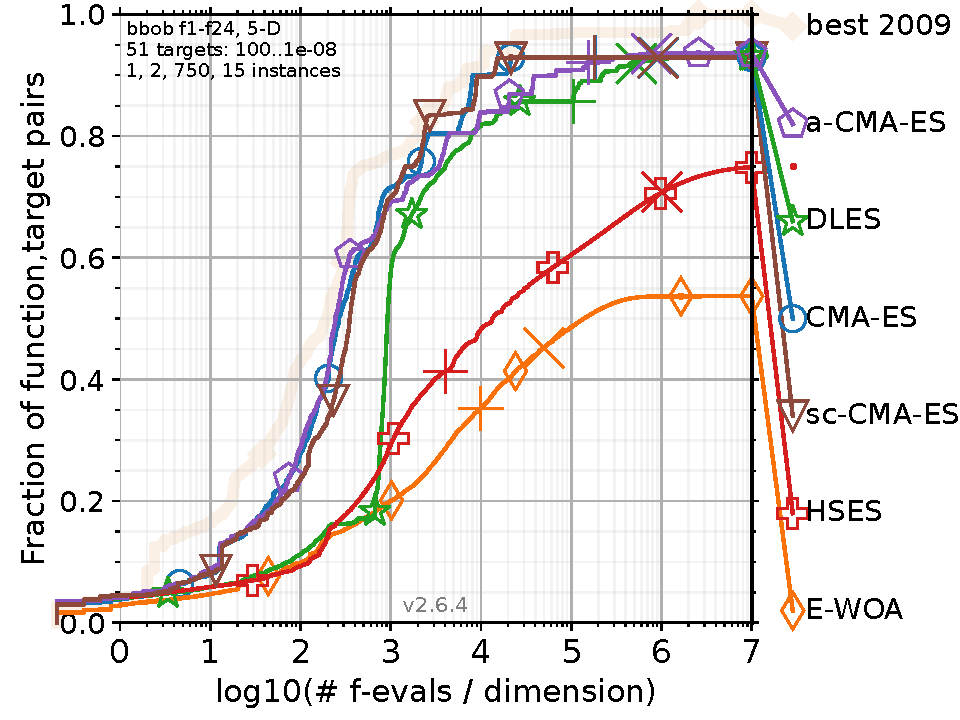
\includegraphics[width=\textwidth]{./bbob/pprldmany_05D_noiselessall.pdf}
	\end{minipage}
	\begin{minipage}[b]{0.3\textwidth}
		\centering
		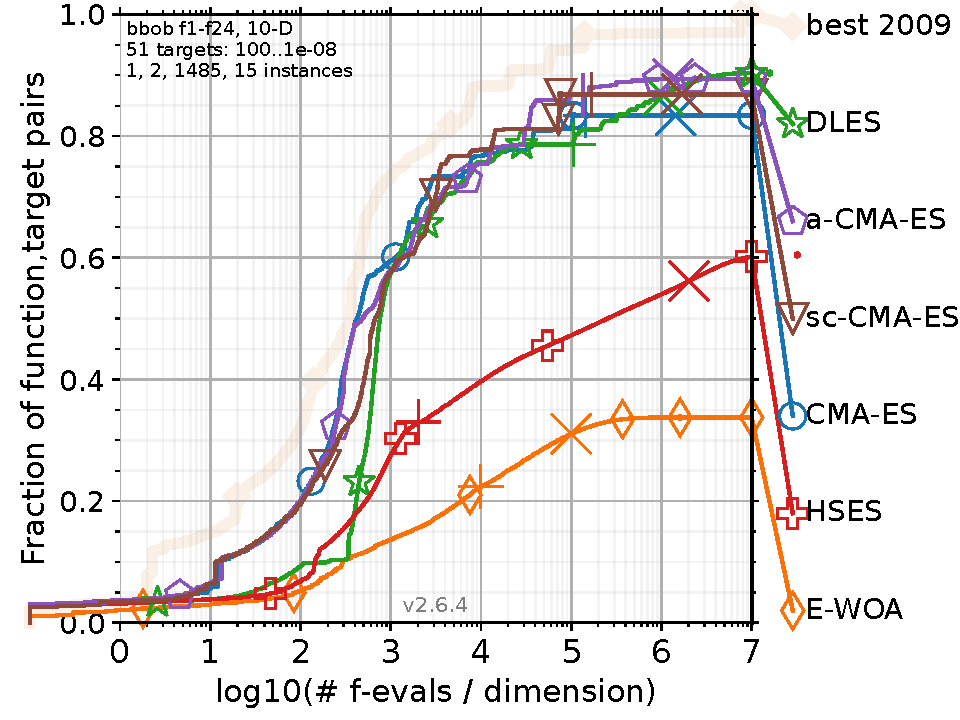
\includegraphics[width=\textwidth]{./bbob/pprldmany_10D_noiselessall.pdf}
	\end{minipage}\hfill
	\begin{minipage}[b]{0.3\textwidth}
		\centering
		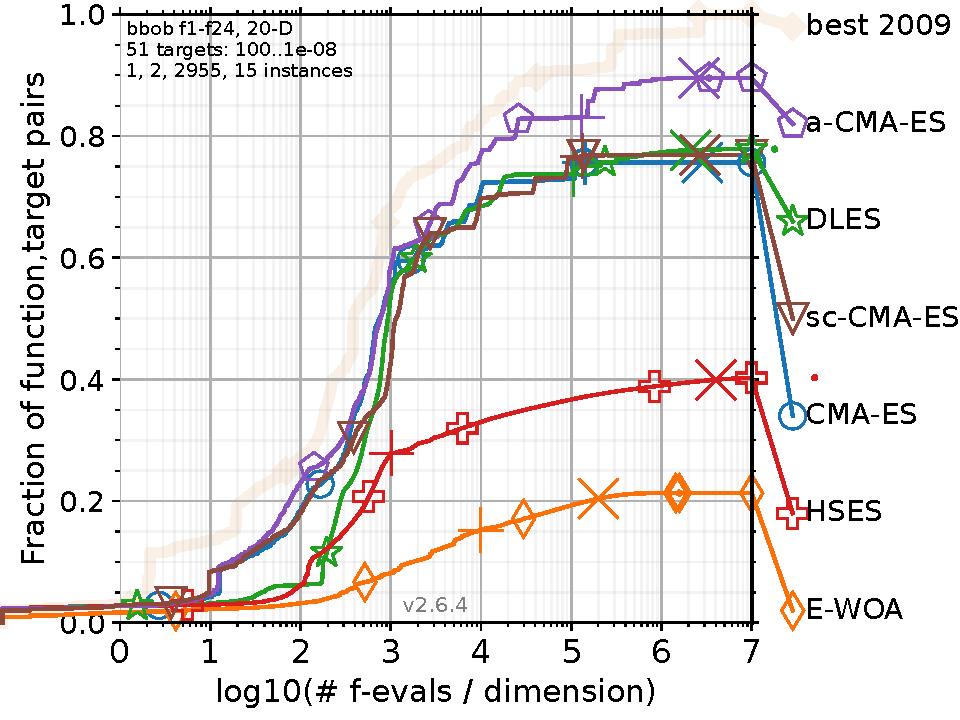
\includegraphics[width=\textwidth]{./bbob/pprldmany_20D_noiselessall.pdf}
	\end{minipage}\hfill
	\begin{minipage}[b]{0.3\textwidth}
		\centering
		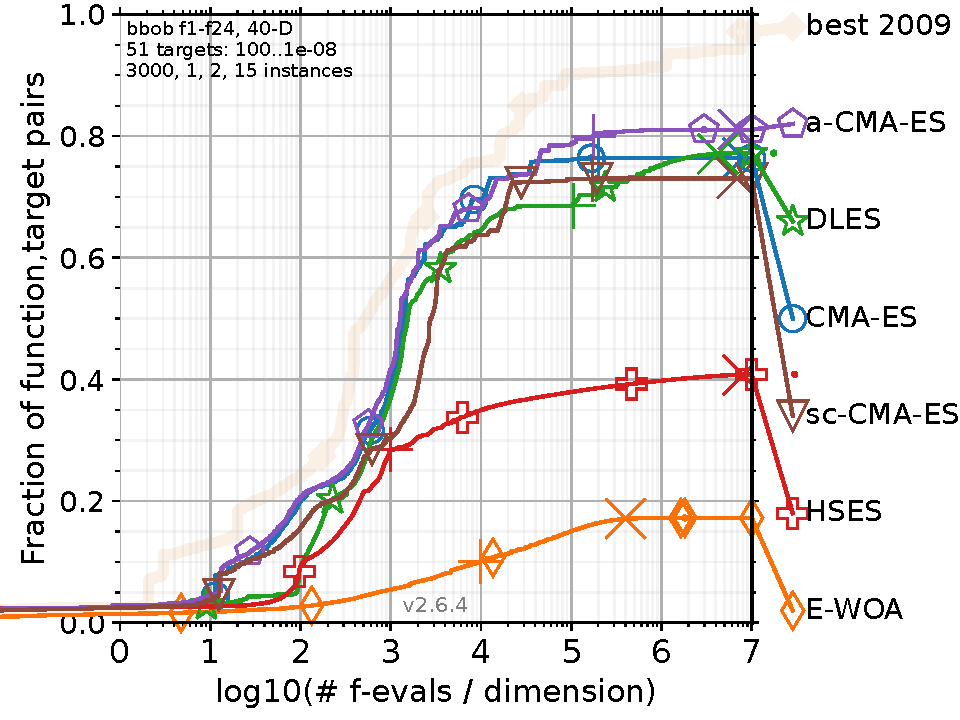
\includegraphics[width=\textwidth]{./bbob/pprldmany_40D_noiselessall.pdf}
	\end{minipage}
	\caption{\textcolor{blue}{Overview of experimental results on the BBOB dataset}}
	\label{bbob-over}
\end{figure}

According to problem types, BBOB divides its 24 functions into 5 categories: Separable Functions (F1-F5), Functions with Low or Moderate Conditioning (F6-F9), Functions with High Conditioning and Unimodal Structure (F10-F14), Multi-modal Functions with Adequate Global Structure (F15-F19), and Multi-modal Functions with Weak Global Structure (F20-F24). The Fig. \ref{bbob-f} present a summary of DLES and its competing algorithms across each category. The first five figures correspond to the five problem categories, while the sixth figure provides an overall summary across all problems, using 10-dimensional cases as an example. 

It is evident that DLES demonstrates outstanding performance in the category of Multi-modal Functions with Weak Global Structure. Compared to other competing algorithms, DLES consistently maintains superior convergence speed and identifies better solutions. This indicates its strong global exploration capability, effectively avoiding local optima and gradually approaching the global optimum in complex search spaces. DLES efficiently handles the complexity of search spaces and maintains stable performance even in high-dimensional problems, making it particularly suitable for optimization problems with complex multimodal characteristics, especially in scenarios lacking clear global trends.

\begin{figure}[H]
	\centering
	\begin{minipage}[b]{0.3\textwidth}
		\centering
		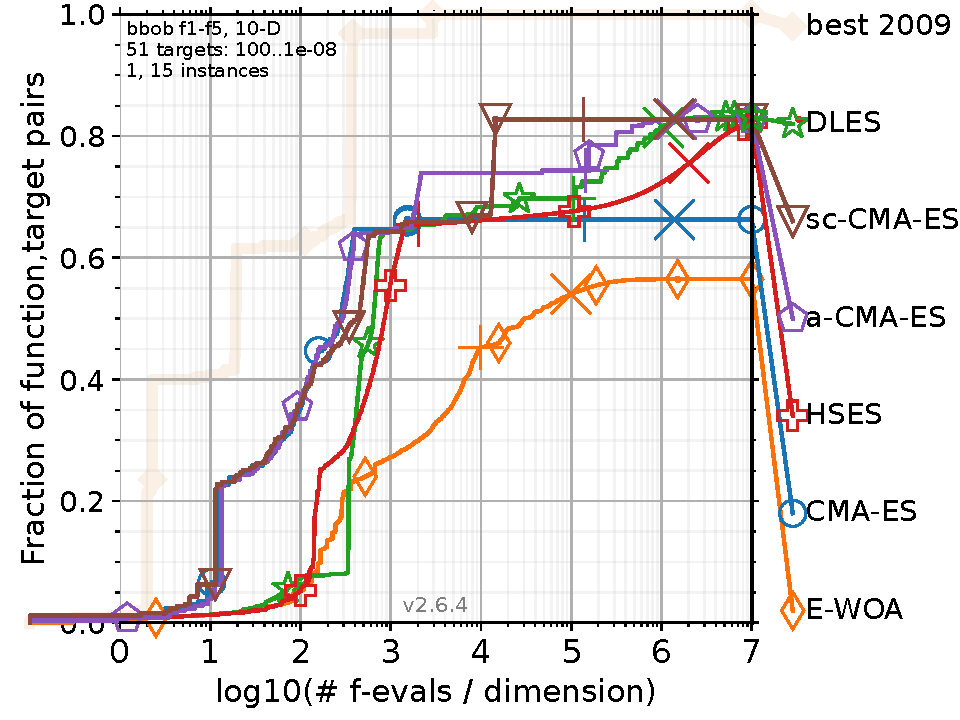
\includegraphics[width=\textwidth]{./bbob/pprldmany_10D_separ.pdf}
	\end{minipage}\hfill
	\begin{minipage}[b]{0.3\textwidth}
		\centering
		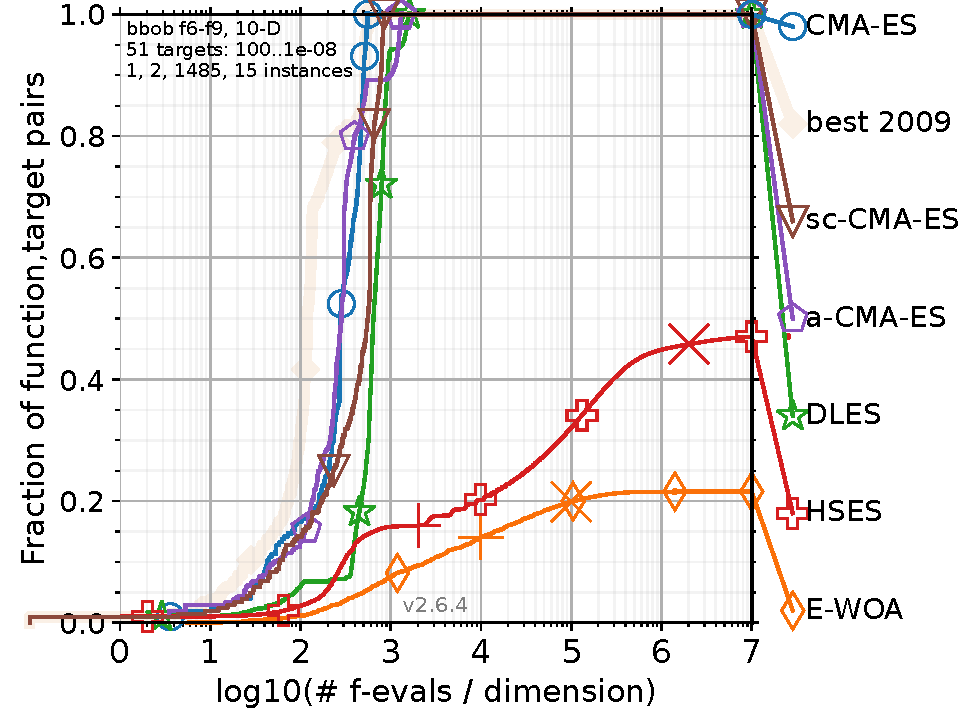
\includegraphics[width=\textwidth]{./bbob/pprldmany_10D_lcond.pdf}
	\end{minipage}\hfill
	\begin{minipage}[b]{0.3\textwidth}
		\centering
		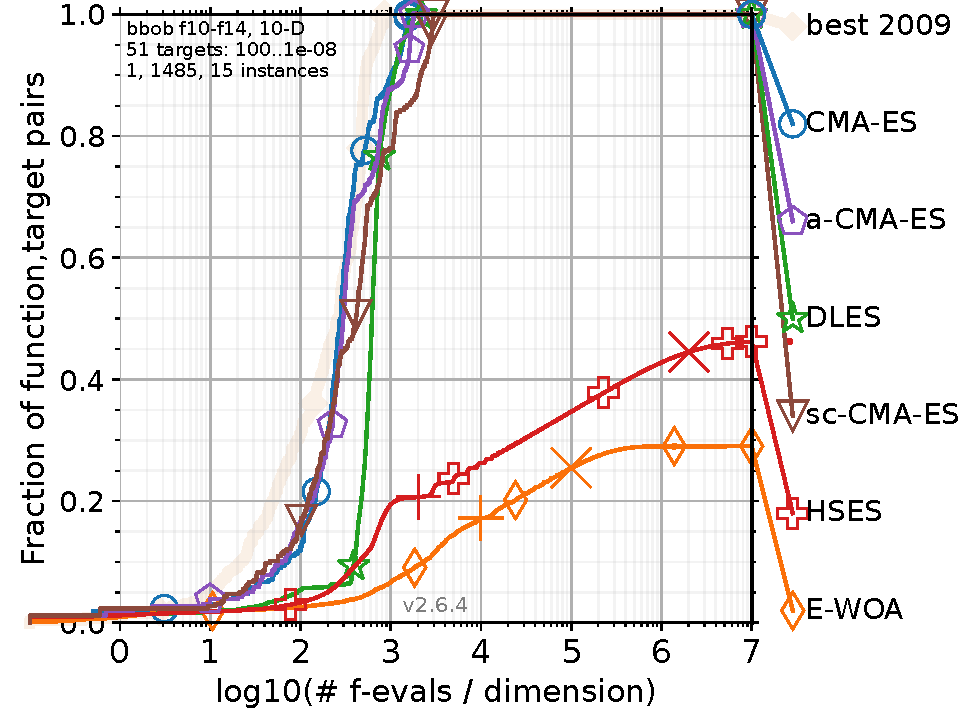
\includegraphics[width=\textwidth]{./bbob/pprldmany_10D_hcond.pdf}
	\end{minipage}
	\begin{minipage}[b]{0.3\textwidth}
		\centering
		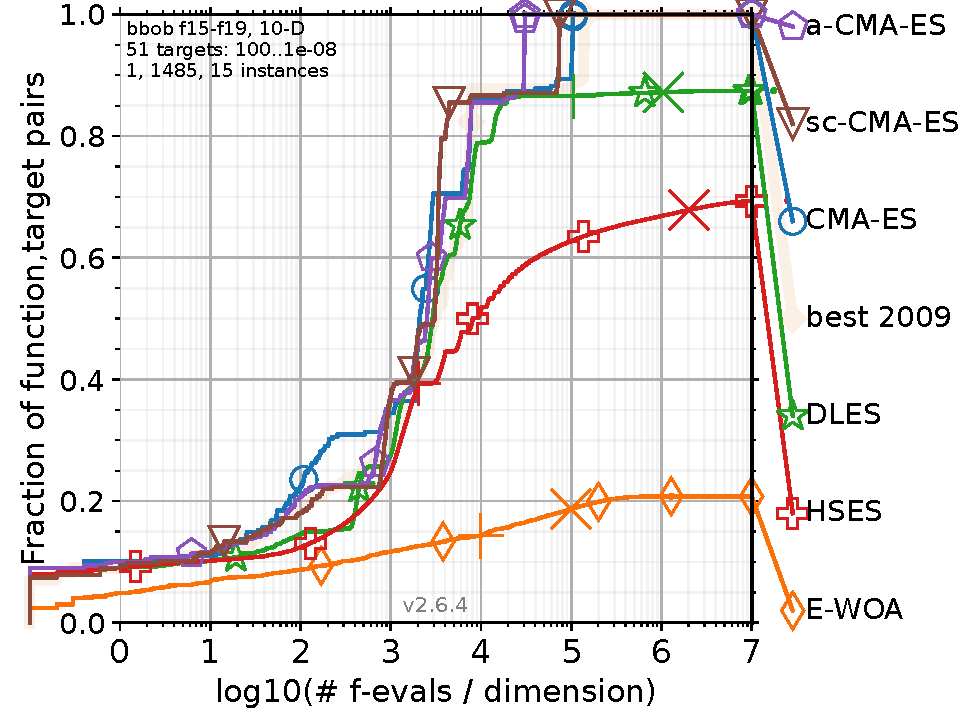
\includegraphics[width=\textwidth]{./bbob/pprldmany_10D_multi.pdf}
	\end{minipage}\hfill
	\begin{minipage}[b]{0.3\textwidth}
		\centering
		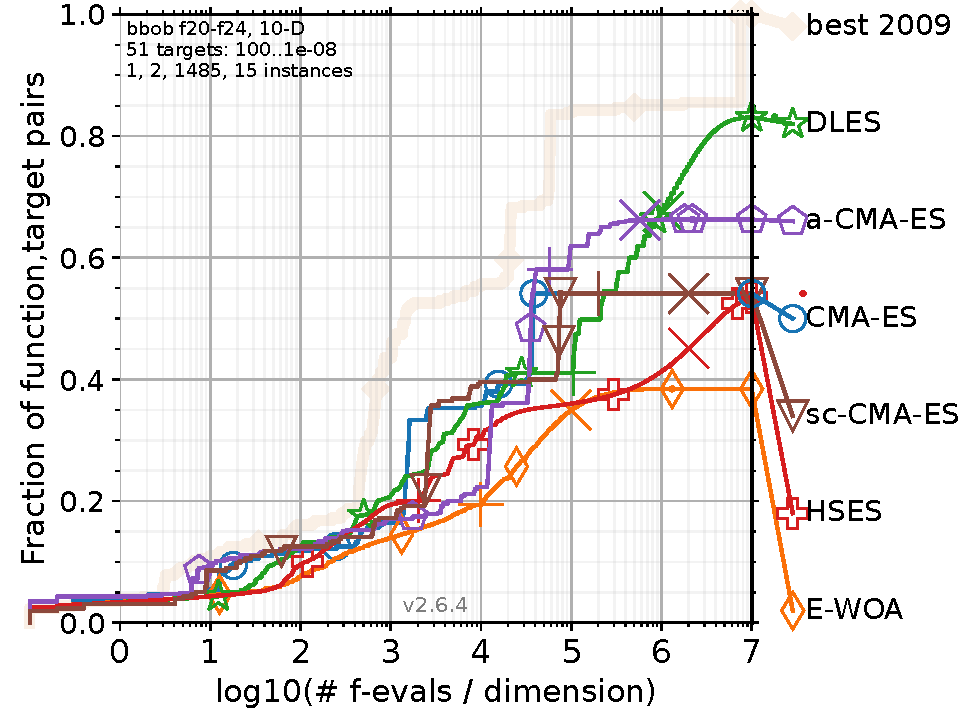
\includegraphics[width=\textwidth]{./bbob/pprldmany_10D_mult2.pdf}
	\end{minipage}\hfill
	\begin{minipage}[b]{0.3\textwidth}
		\centering
		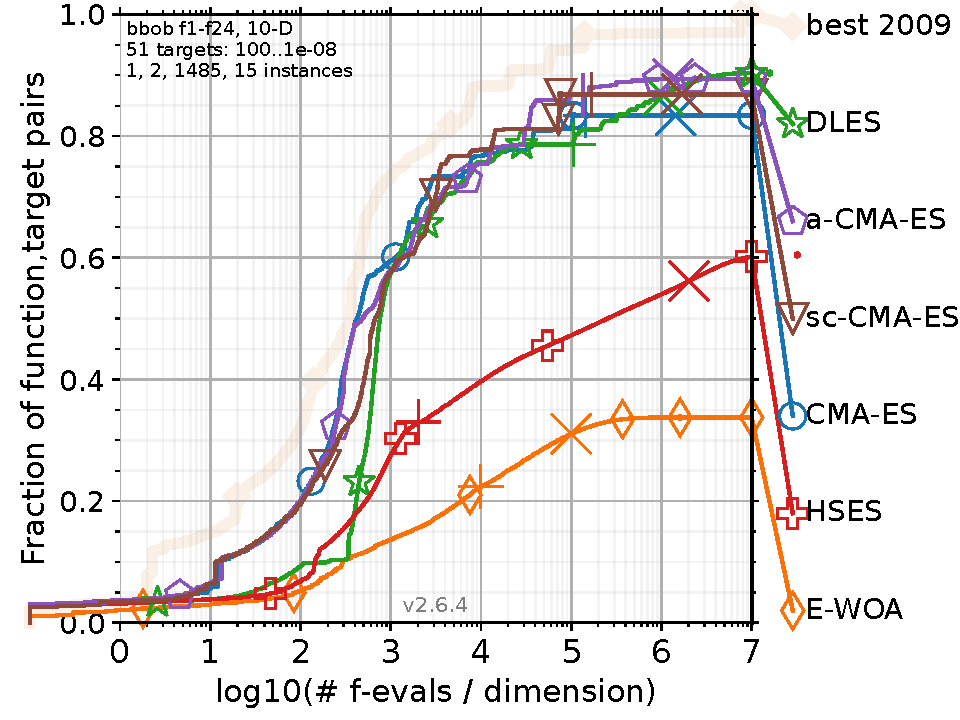
\includegraphics[width=\textwidth]{./bbob/pprldmany_10D_noiselessall.pdf}
	\end{minipage}
	\caption{\textcolor{blue}{Experimental results on the BBOB dataset in $D$ = 10}}
	\label{bbob-f}
\end{figure}

To better illustrate the specific advantages of the DLES algorithm, we select three representative ECDFs plots, F4 Büche-Rastrigin Function, F22 Gallagher's Gaussian 21-hi Peaks Function, and F23 Katsuura Function. These problems are characterized by their highly multimodal nature and complex search spaces, with numerous local optima. Their search landscapes are complex and irregular, often exhibiting asymmetry or non-linear characteristics, which pose challenges to an algorithm's robustness and adaptability.

As shown in Fig. \ref{bbob-exp}, DLES demonstrates remarkable superiority in solving these types of problems, indicating that it is highly effective in handling complex, multimodal, and high-dimensional optimization tasks. Specifically, DLES exhibits strong global search capabilities, allowing it to effectively avoid local optima and steer towards the global optimum. Additionally, it shows excellent adaptability and robustness in managing irregular search spaces. Overall, DLES performs exceptionally well in addressing complex, multimodal, and high-dimensional optimization problems.
\begin{figure}[H]
	\centering
	\begin{minipage}[b]{0.3\textwidth}
		\centering
		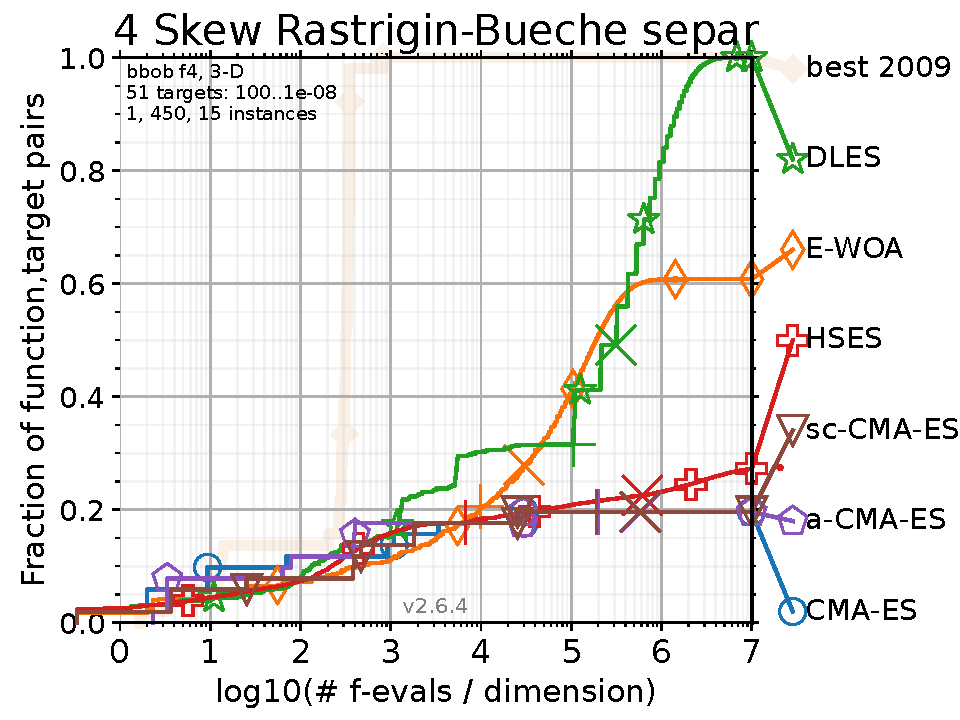
\includegraphics[width=\textwidth]{./bbob/pprldmany_f004_03D.pdf}
	\end{minipage}\hfill
	\begin{minipage}[b]{0.3\textwidth}
		\centering
		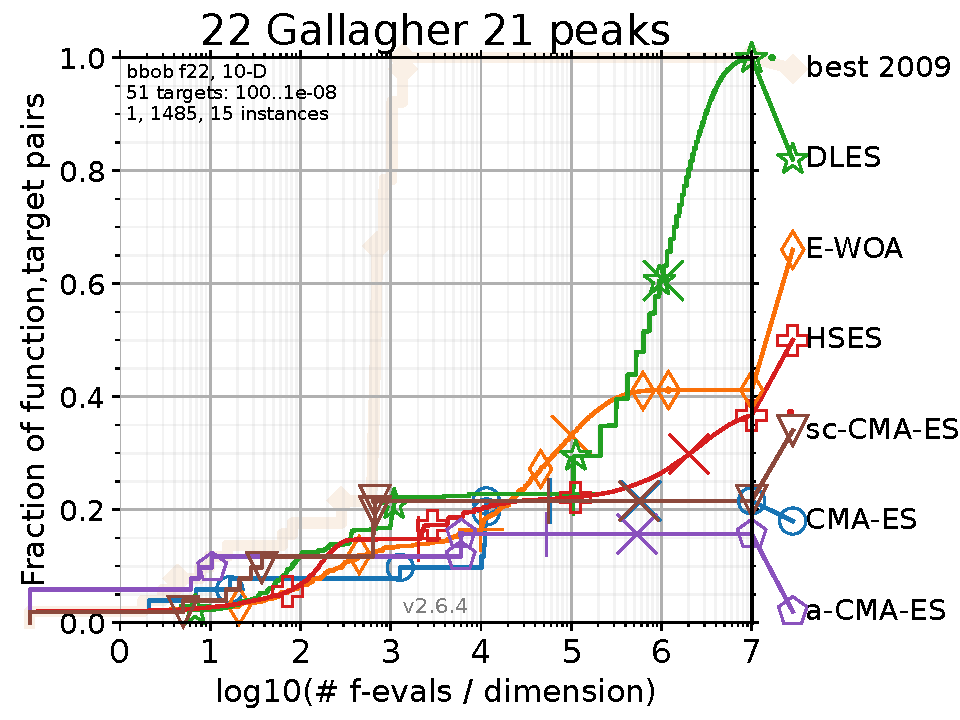
\includegraphics[width=\textwidth]{./bbob/pprldmany_f022_10D.pdf}
	\end{minipage}\hfill
	\begin{minipage}[b]{0.3\textwidth}
		\centering
		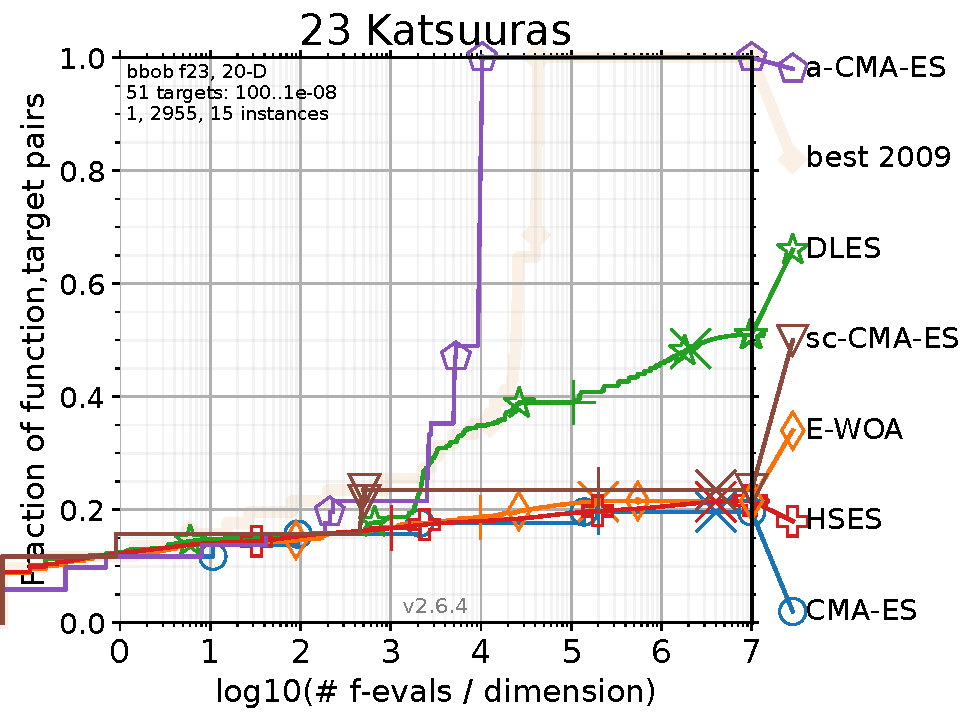
\includegraphics[width=\textwidth]{./bbob/pprldmany_f023_20D.pdf}
	\end{minipage}
	\caption{\textcolor{blue}{Experimental results of F4, F22, and F23 on the BBOB dataset}}
	\label{bbob-exp}
\end{figure}

\section{Supplementary Experimental Results}\label{a-r}
As shown in Table~\ref{parameter}, the parameter settings of algorithms are configured as the recommended values according to the references. Fig. \ref{b-p-start}\textemdash Fig. \ref{b-p-end} display the average convergence curves and box plots for DLES and nine comparison algorithms across all problems in the CEC 2018 dataset. Fig. \ref{bbob-start}\textemdash \ref{bbob-end} illustrate the runtime distributions (ECDFs) of DLES and five comparison algorithms across all problems in the BBOB dataset. Tables~\ref{CEC2014_10}\textemdash \ref{CEC2014_100} present the consolidated experimental results of DLES and state-of-the-art competitive algorithms on CEC 2014 benchmark functions across dimensions 10, 30, 50, and 100. Similarly, Tables~\ref{CEC2018_10}\textemdash \ref{CEC2018_100} showcase the summarized experimental outcomes of DLES and leading competitive algorithms on CEC 2018 benchmark functions in the same dimensions. Additionally, Table~\ref{CEC2022_10} and Table~\ref{CEC2022_20} exhibit the consolidated experimental findings of DLES and state-of-the-art competitive algorithms on CEC 2022 benchmark functions in dimensions 10 and 20, respectively.

\begin{table}[h]
	\centering
	\caption{The detail parameter settings of the experimental group.}
	\label{parameter}
	\begin{tabular}{ll}
		\hline
		Algorithm          &  Settings \\
		\hline
		DLES    &    $N_i=100, T=100, E=10, lr=0.5, cc=0.96$ \\
		CMAES     &    $N_i=100, \sigma=0.25 , \lambda = 10, \mu = 5 $ \\
		DDE-ARA  &  $N_1=100, N_2=50, C_r=[0.1,0.9], F=0.7$ \\
		EA4eig     &    $N_i=100, N_m=10, q_h=1/4, F_0=0.7, C_{r0}=0.9$ \\
		HSES  &  $N_1=100, T=100, \lambda = \lfloor 3 \ln D \rfloor + 80,  cc=0.96 $ \\
		LSHADE  &   $N_i=18\times D, N_m=4, p=0.11, A_r=2.6, K=5$ \\ 
		TAPSO  &  $N_i=100, w=0.7298, p_c=0.5, p_m=0.5, M=N/4$ \\
		MLGSA  &  $N_i=100, s=100, n=3/2, p_m=0.5, l=2$ \\ \hline
		LEO-PSO  &  $N_i=100, arch_size=100, lr=0.01, \alpha = 0.5, \beta=0.9 $\\
		QHSES  &  $N_i=100, T=20, \alpha = 0.0001, maxE = 5000$ \\
		\hline
	\end{tabular}
\end{table}
%----------------------------------------BBOB----------------------------------------------------------
%第一组图像
\begin{figure}[H]
	\centering
	\begin{minipage}[b]{0.32\textwidth}
		\centering
		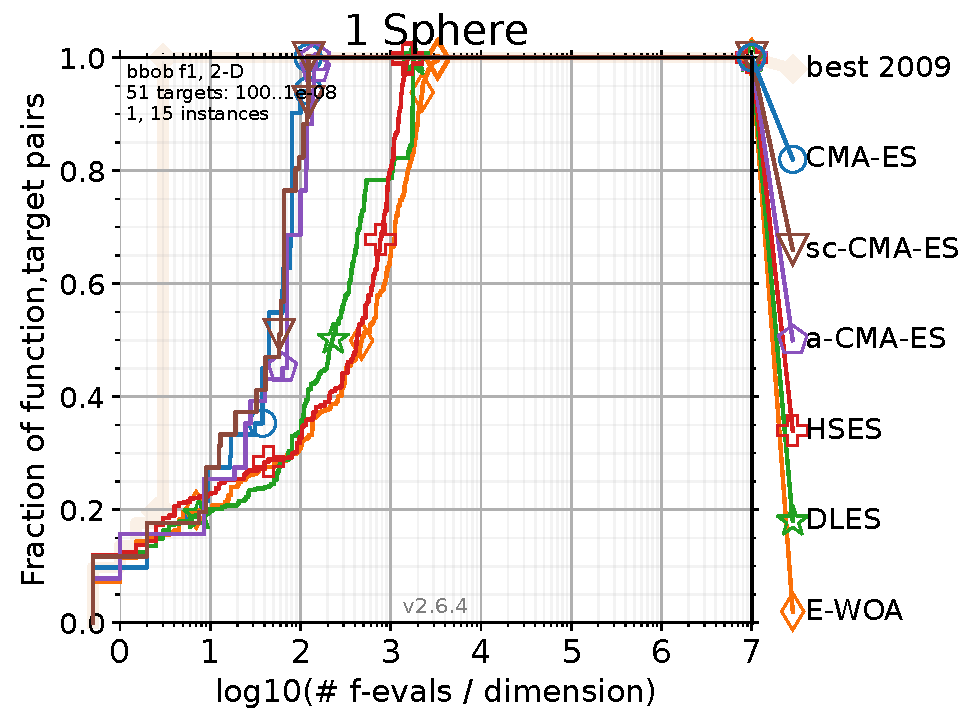
\includegraphics[width=\textwidth]{./bbob/pprldmany_f001_02D.pdf}
	\end{minipage}\hfill
	\begin{minipage}[b]{0.32\textwidth}
		\centering
		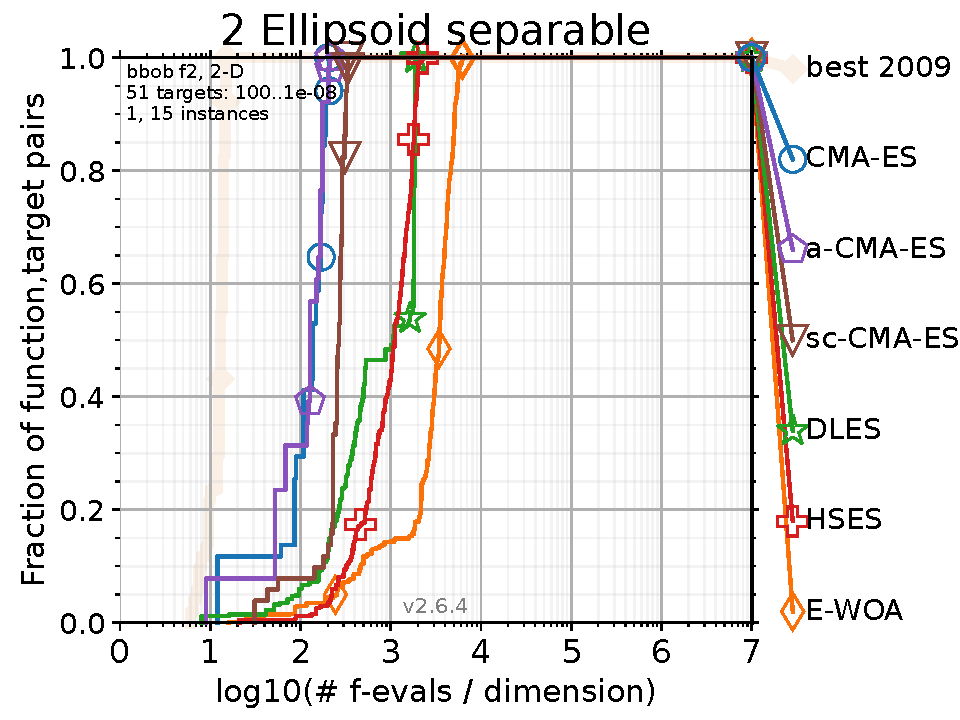
\includegraphics[width=\textwidth]{./bbob/pprldmany_f002_02D.pdf}
	\end{minipage}\hfill
	\begin{minipage}[b]{0.32\textwidth}
		\centering
		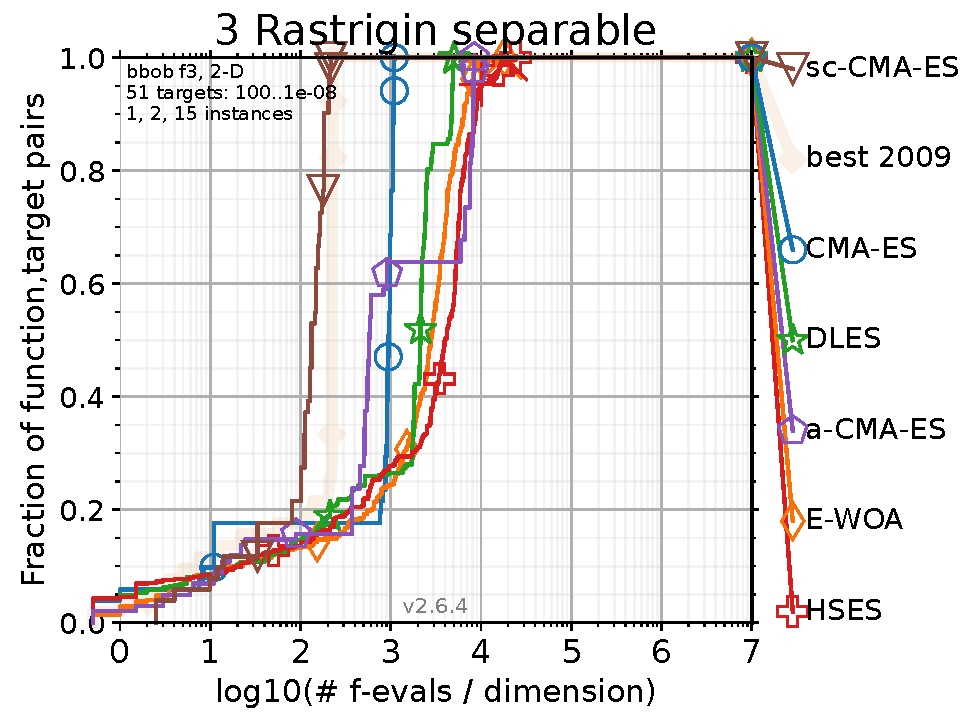
\includegraphics[width=\textwidth]{./bbob/pprldmany_f003_02D.pdf}
	\end{minipage}
	\caption{\textcolor{blue}{F1 to F3 in $D$ = 2.}}
	\label{bbob-start}
\end{figure}

% 第二组图像
\begin{figure}[H]
	\centering
	\begin{minipage}[b]{0.32\textwidth}
		\centering
		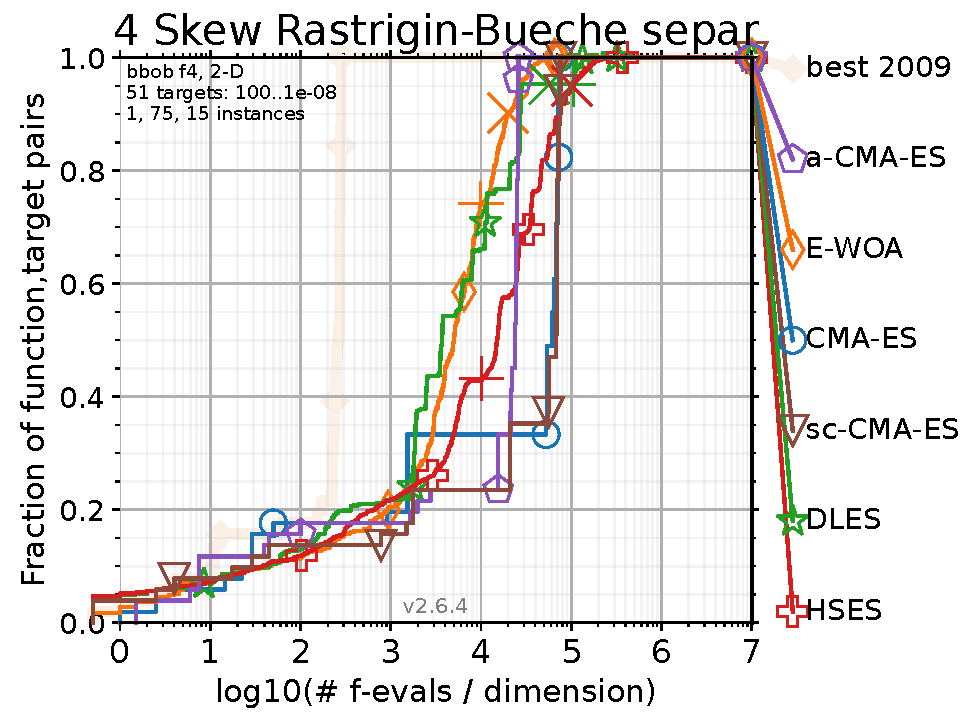
\includegraphics[width=\textwidth]{./bbob/pprldmany_f004_02D.pdf}
	\end{minipage}\hfill
	\begin{minipage}[b]{0.32\textwidth}
		\centering
		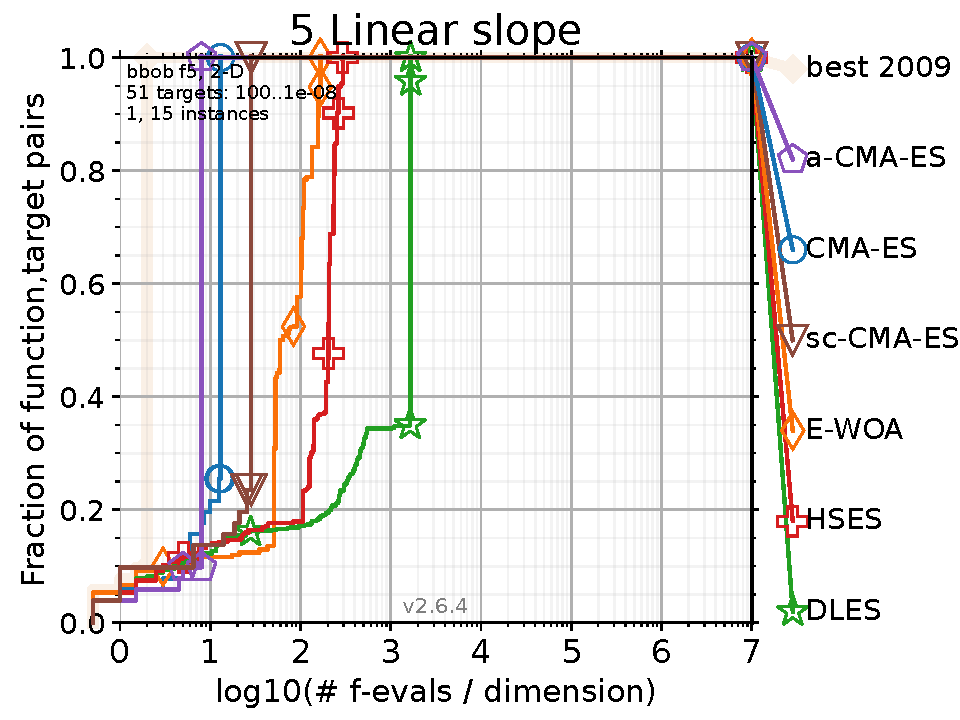
\includegraphics[width=\textwidth]{./bbob/pprldmany_f005_02D.pdf}
	\end{minipage}\hfill
	\begin{minipage}[b]{0.32\textwidth}
		\centering
		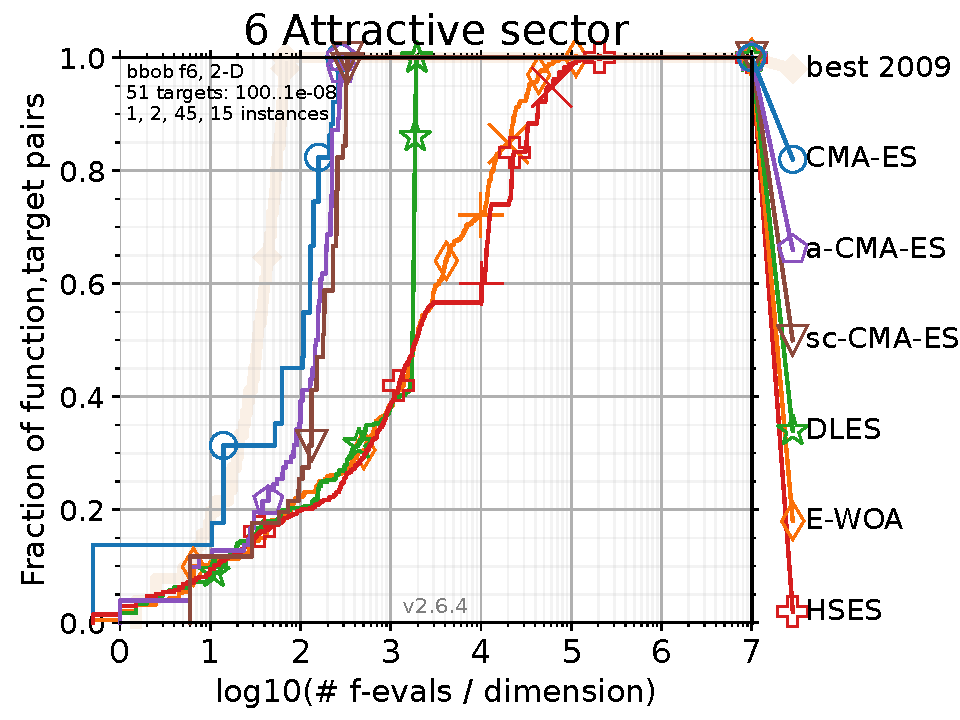
\includegraphics[width=\textwidth]{./bbob/pprldmany_f006_02D.pdf}
	\end{minipage}
	\caption{\textcolor{blue}{F4 to F6 in $D$ = 2.}}
\end{figure}

% 第三组图像
\begin{figure}[H]
	\centering
	\begin{minipage}[b]{0.32\textwidth}
		\centering
		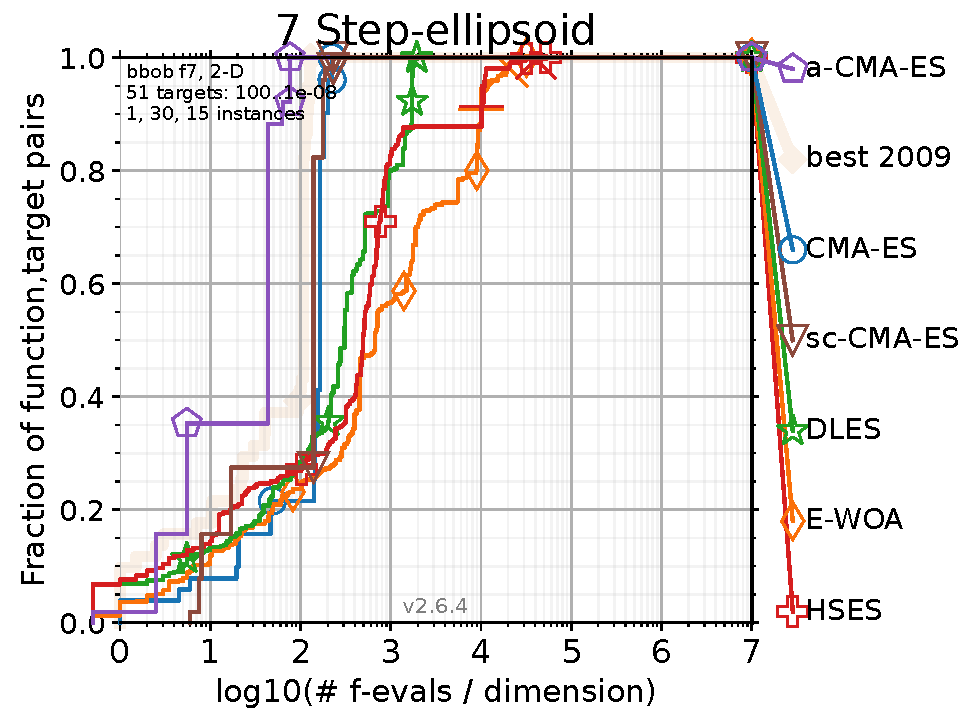
\includegraphics[width=\textwidth]{./bbob/pprldmany_f007_02D.pdf}
	\end{minipage}\hfill
	\begin{minipage}[b]{0.32\textwidth}
		\centering
		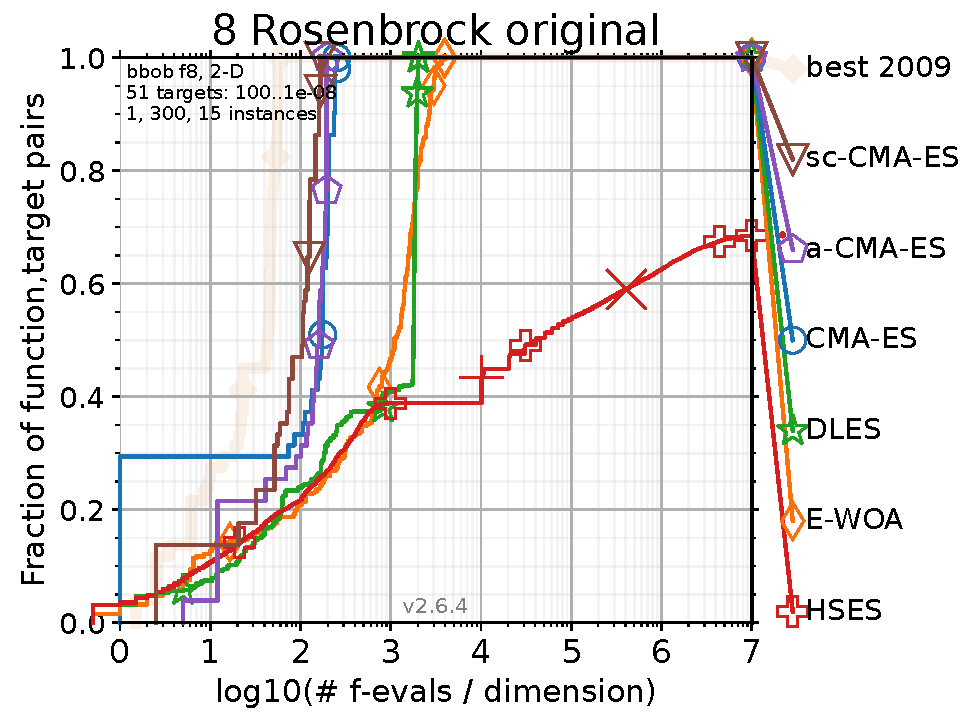
\includegraphics[width=\textwidth]{./bbob/pprldmany_f008_02D.pdf}
	\end{minipage}\hfill
	\begin{minipage}[b]{0.32\textwidth}
		\centering
		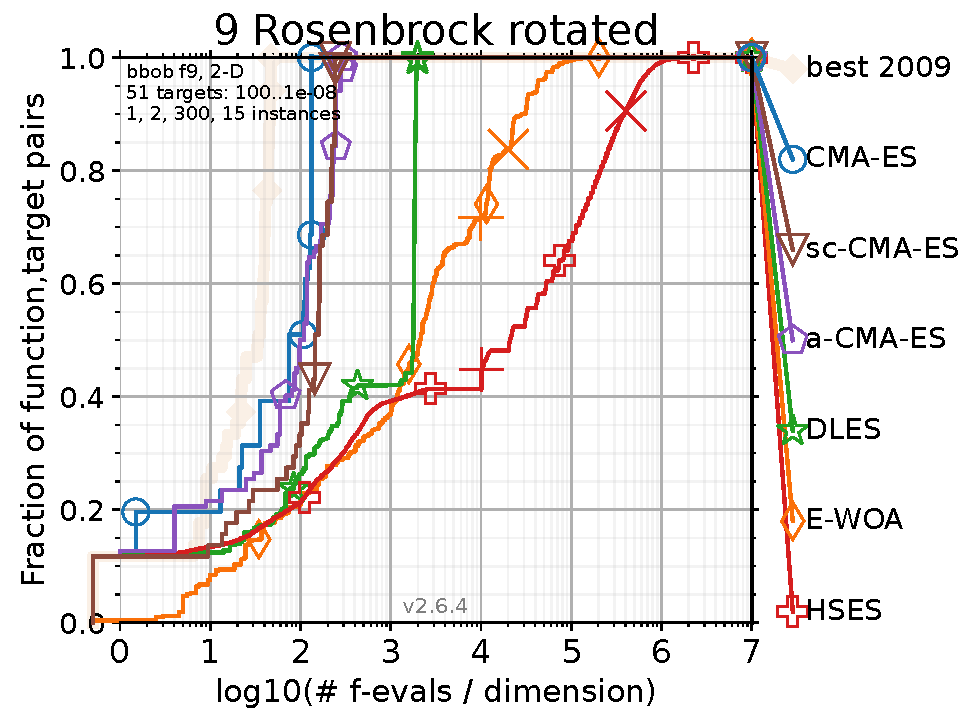
\includegraphics[width=\textwidth]{./bbob/pprldmany_f009_02D.pdf}
	\end{minipage}
	\caption{\textcolor{blue}{F7 to F9 in $D$ = 2.}}
\end{figure}

% 第四组图像
\begin{figure}[H]
	\centering
	\begin{minipage}[b]{0.32\textwidth}
		\centering
		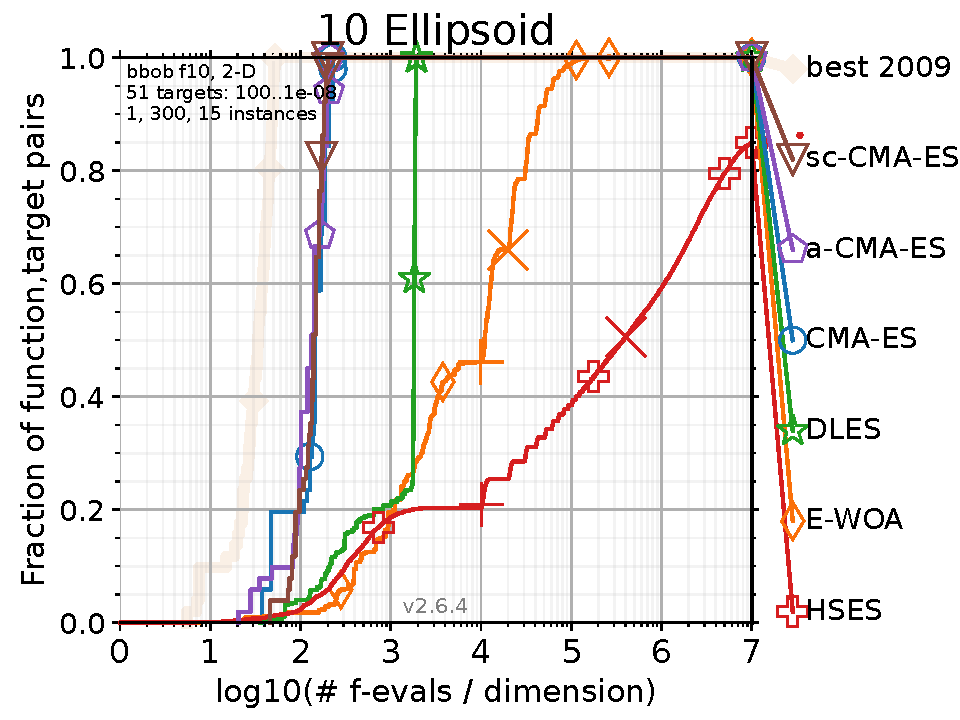
\includegraphics[width=\textwidth]{./bbob/pprldmany_f010_02D.pdf}
	\end{minipage}\hfill
	\begin{minipage}[b]{0.32\textwidth}
		\centering
		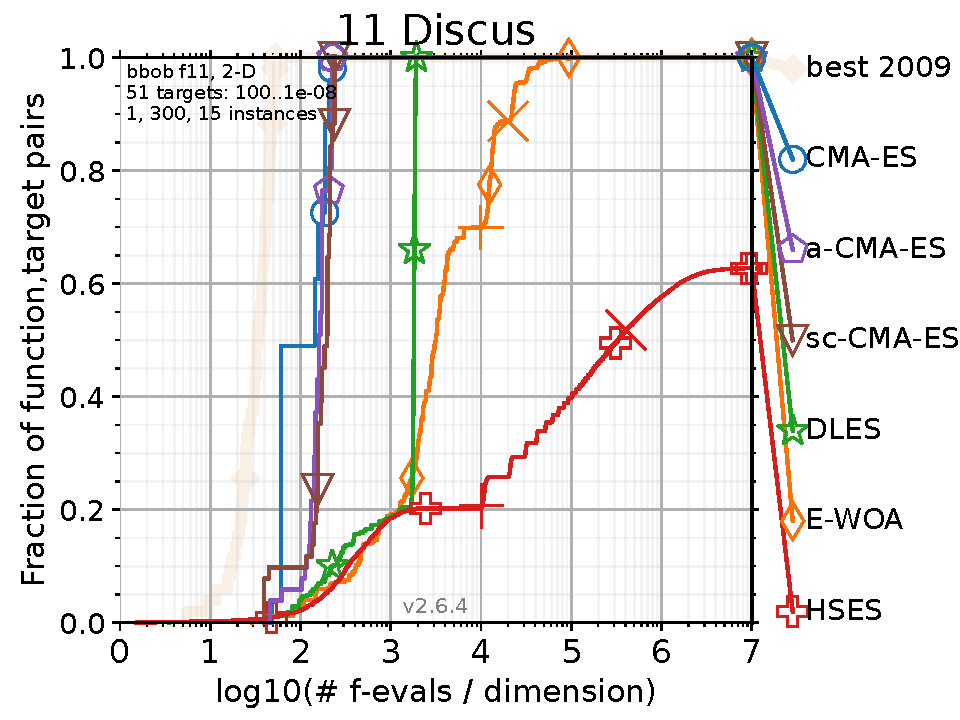
\includegraphics[width=\textwidth]{./bbob/pprldmany_f011_02D.pdf}
	\end{minipage}\hfill
	\begin{minipage}[b]{0.32\textwidth}
		\centering
		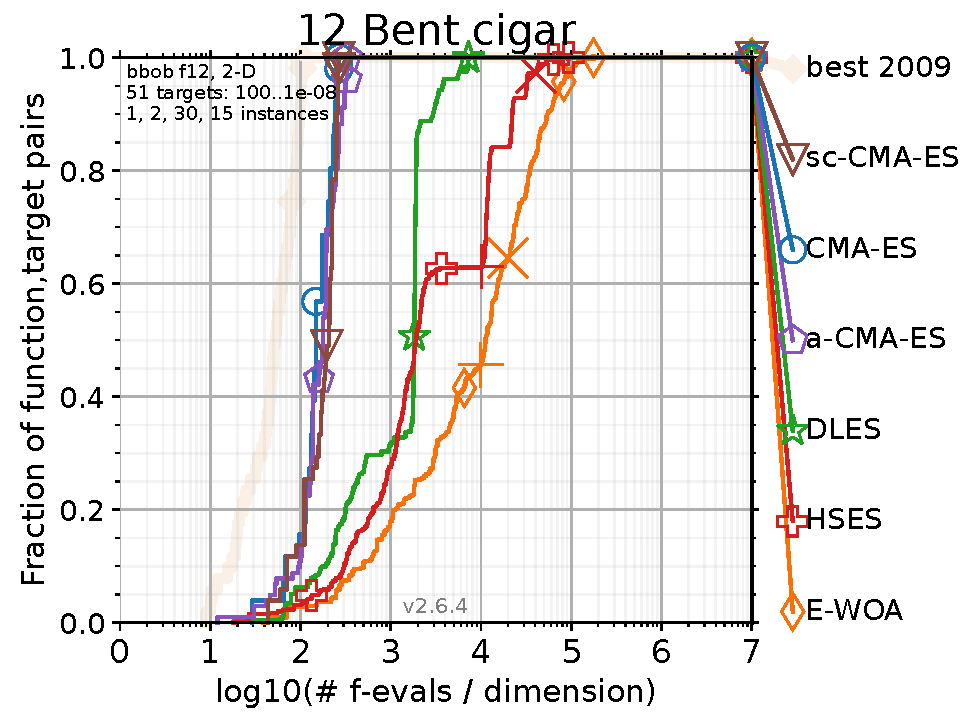
\includegraphics[width=\textwidth]{./bbob/pprldmany_f012_02D.pdf}
	\end{minipage}
	\caption{\textcolor{blue}{F10 to F12 in $D$ = 2.}}
\end{figure}

% 第五组图像
\begin{figure}[H]
	\centering
	\begin{minipage}[b]{0.32\textwidth}
		\centering
		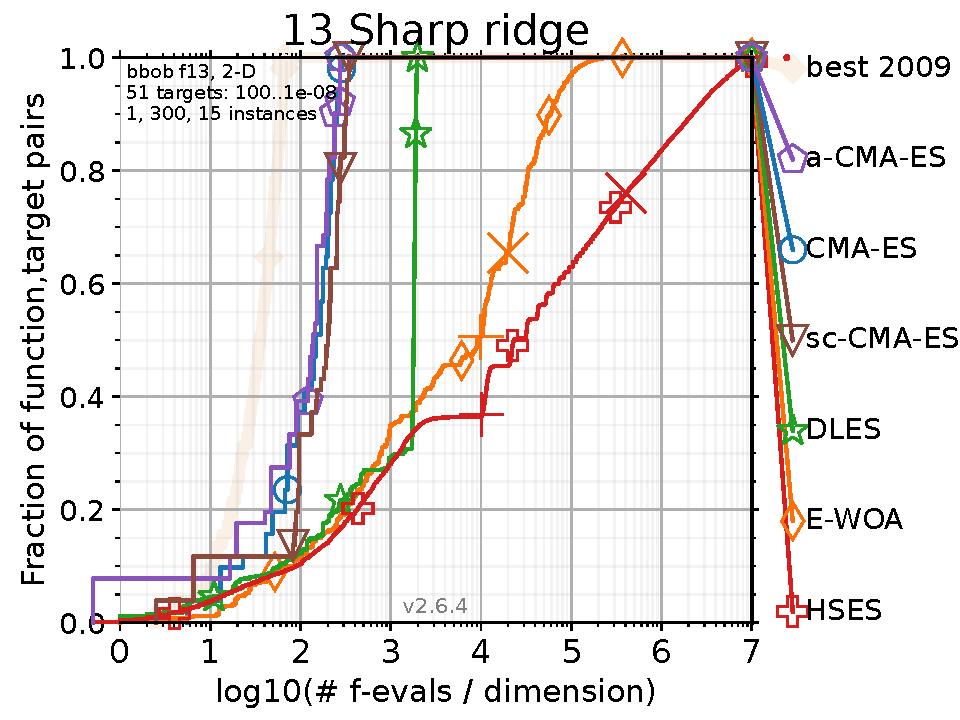
\includegraphics[width=\textwidth]{./bbob/pprldmany_f013_02D.pdf}
	\end{minipage}\hfill
	\begin{minipage}[b]{0.32\textwidth}
		\centering
		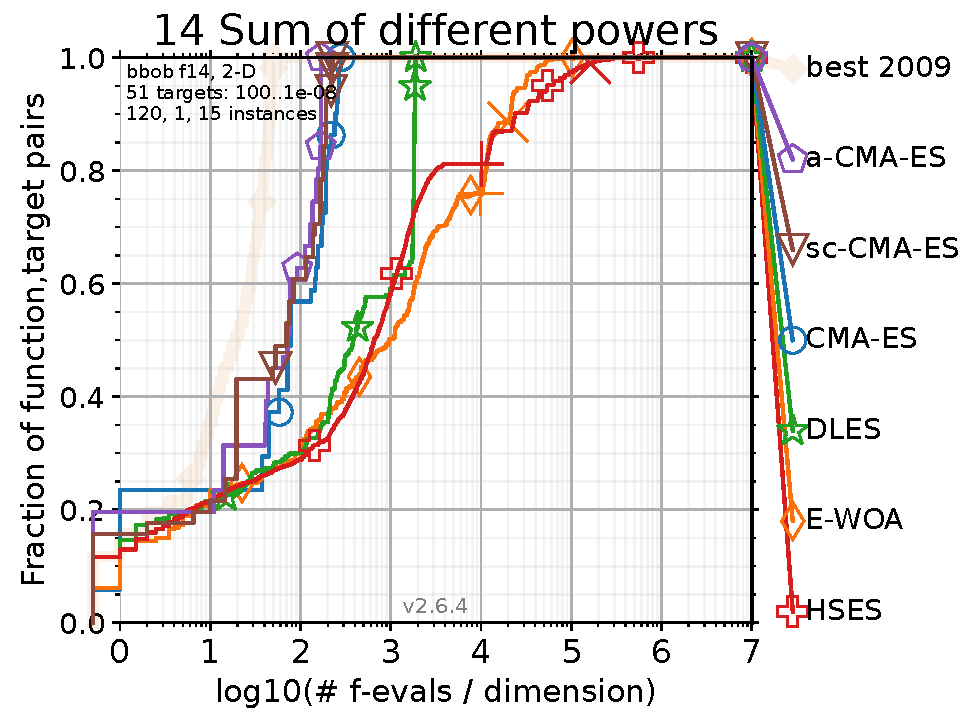
\includegraphics[width=\textwidth]{./bbob/pprldmany_f014_02D.pdf}
	\end{minipage}\hfill
	\begin{minipage}[b]{0.32\textwidth}
		\centering
		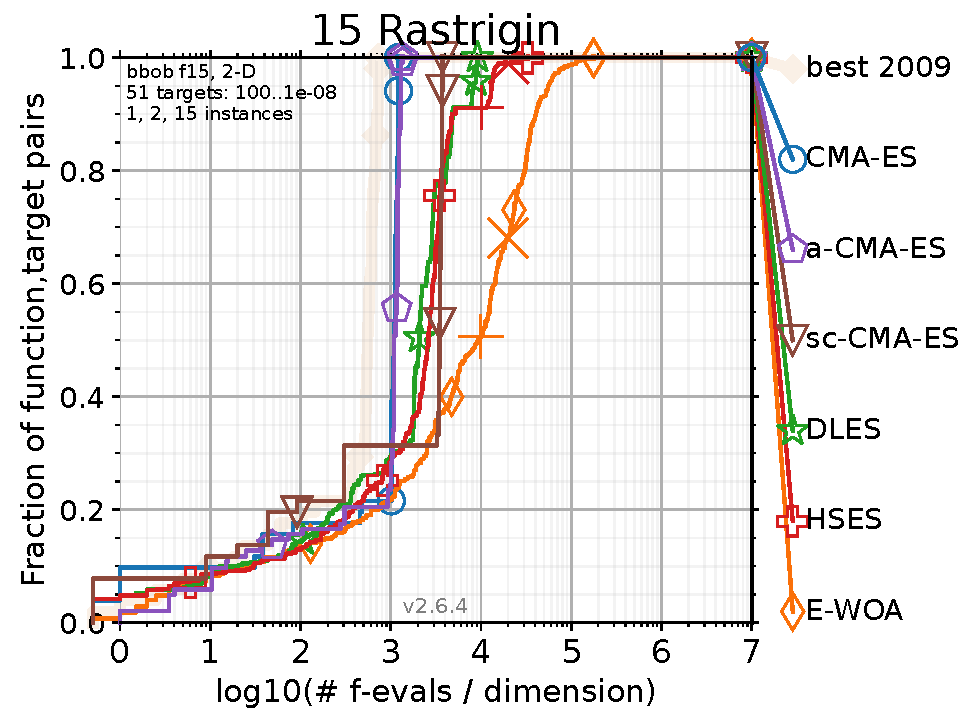
\includegraphics[width=\textwidth]{./bbob/pprldmany_f015_02D.pdf}
	\end{minipage}
	\caption{\textcolor{blue}{F13 to F15 in $D$ = 2.}}
\end{figure}

% 第六组图像
\begin{figure}[H]
	\centering
	\begin{minipage}[b]{0.32\textwidth}
		\centering
		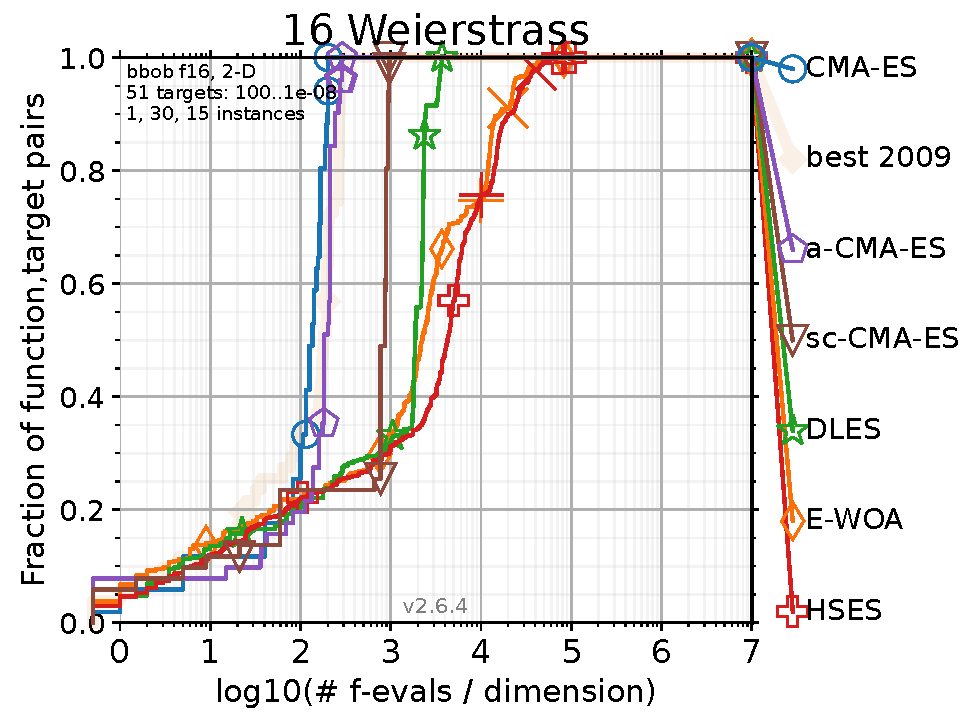
\includegraphics[width=\textwidth]{./bbob/pprldmany_f016_02D.pdf}
	\end{minipage}\hfill
	\begin{minipage}[b]{0.32\textwidth}
		\centering
		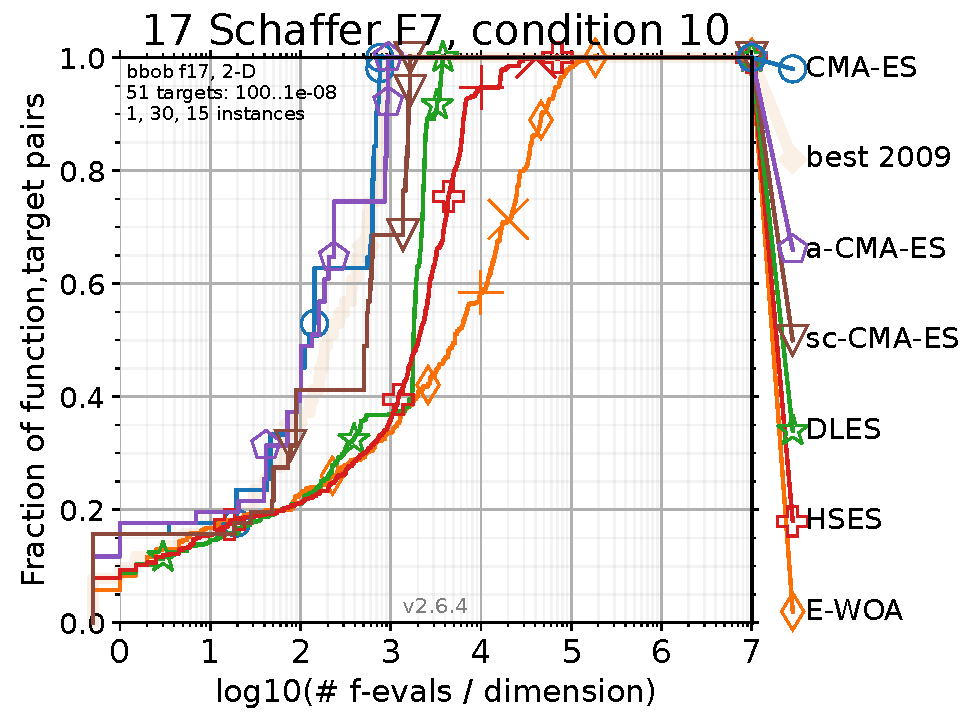
\includegraphics[width=\textwidth]{./bbob/pprldmany_f017_02D.pdf}
	\end{minipage}\hfill
	\begin{minipage}[b]{0.32\textwidth}
		\centering
		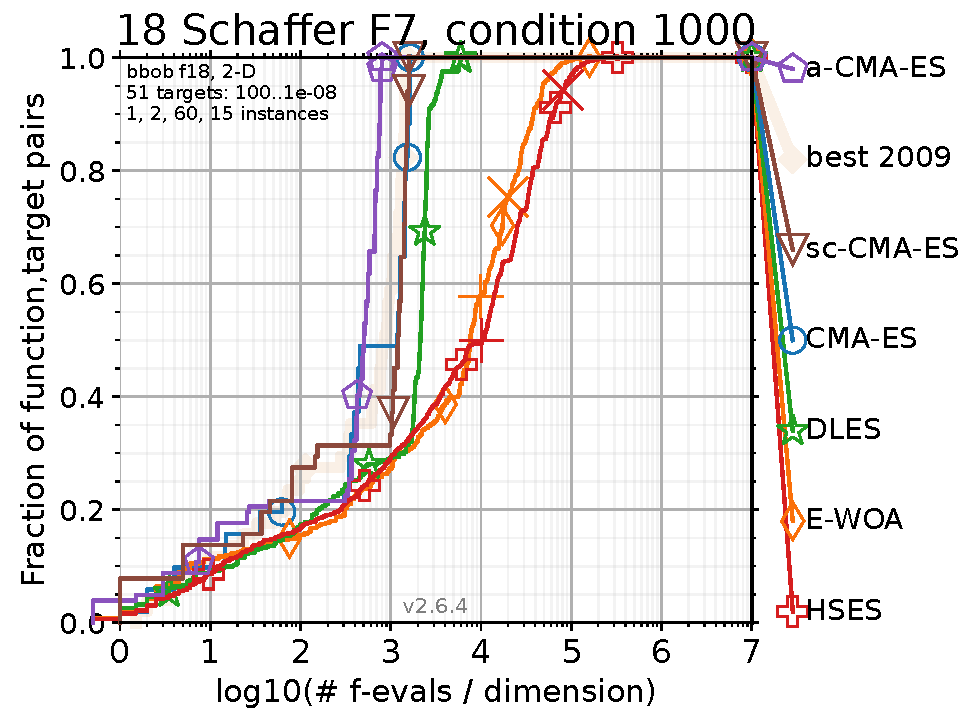
\includegraphics[width=\textwidth]{./bbob/pprldmany_f018_02D.pdf}
	\end{minipage}
	\caption{\textcolor{blue}{F16 to F18 in $D$ = 2.}}
\end{figure}

% 第七组图像
\begin{figure}[H]
	\centering
	\begin{minipage}[b]{0.32\textwidth}
		\centering
		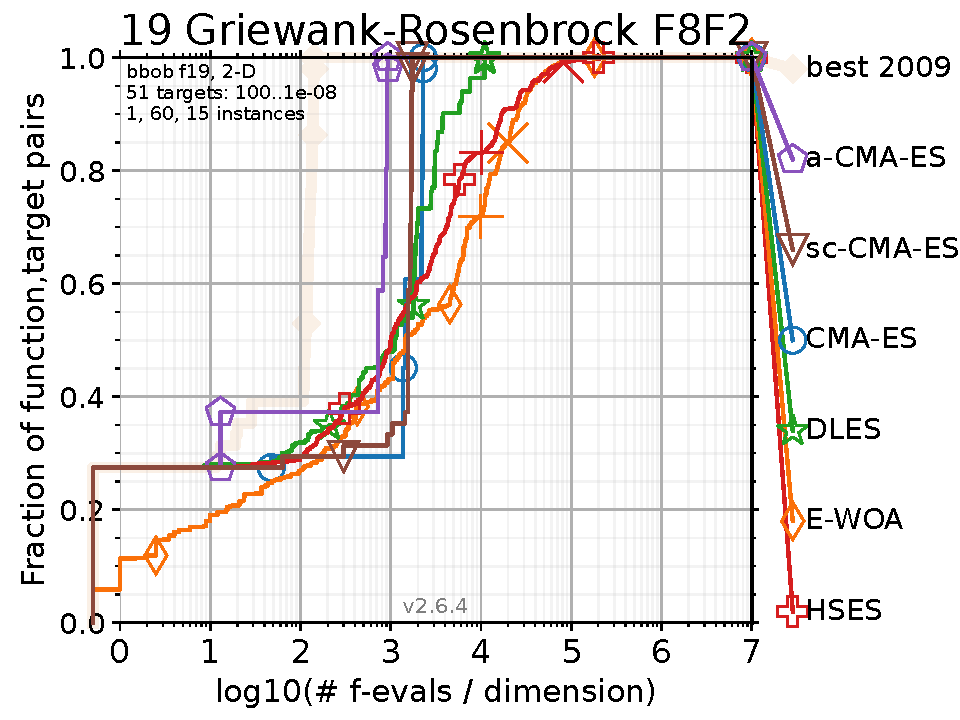
\includegraphics[width=\textwidth]{./bbob/pprldmany_f019_02D.pdf}
	\end{minipage}\hfill
	\begin{minipage}[b]{0.32\textwidth}
		\centering
		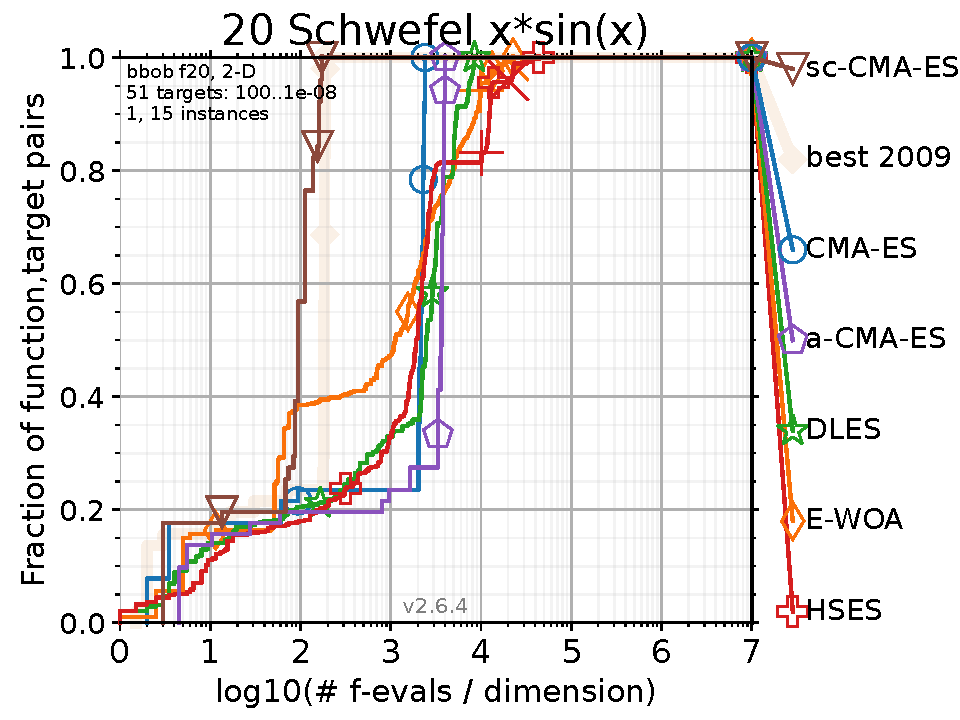
\includegraphics[width=\textwidth]{./bbob/pprldmany_f020_02D.pdf}
	\end{minipage}\hfill
	\begin{minipage}[b]{0.32\textwidth}
		\centering
		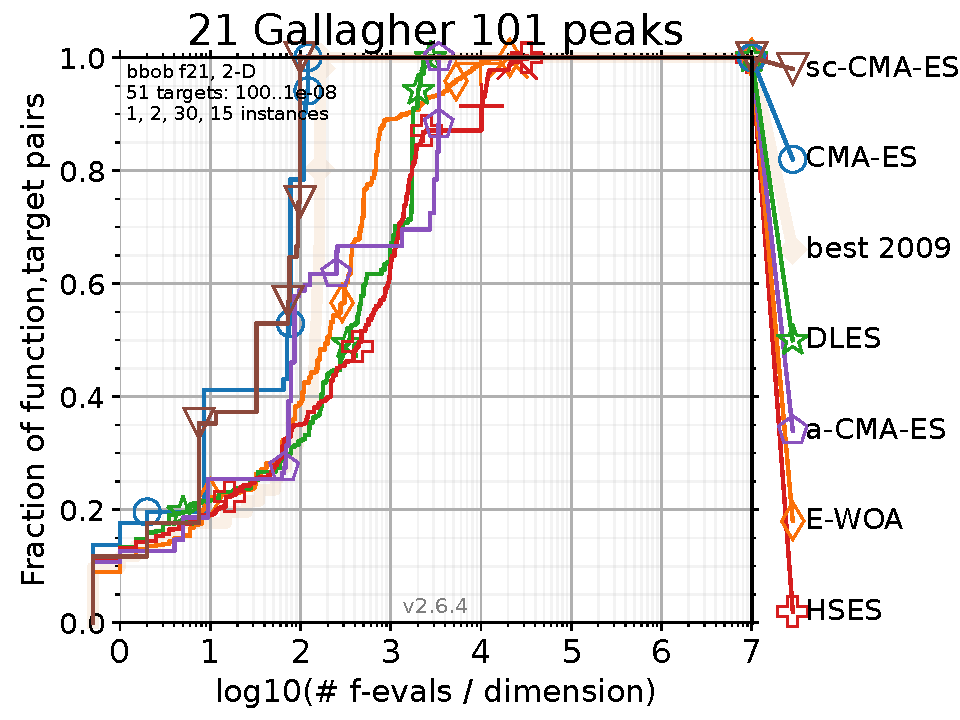
\includegraphics[width=\textwidth]{./bbob/pprldmany_f021_02D.pdf}
	\end{minipage}
	\caption{\textcolor{blue}{F19 to F21 in $D$ = 2.}}
\end{figure}

% 第八组图像
\begin{figure}[H]
	\centering
	\begin{minipage}[b]{0.32\textwidth}
		\centering
		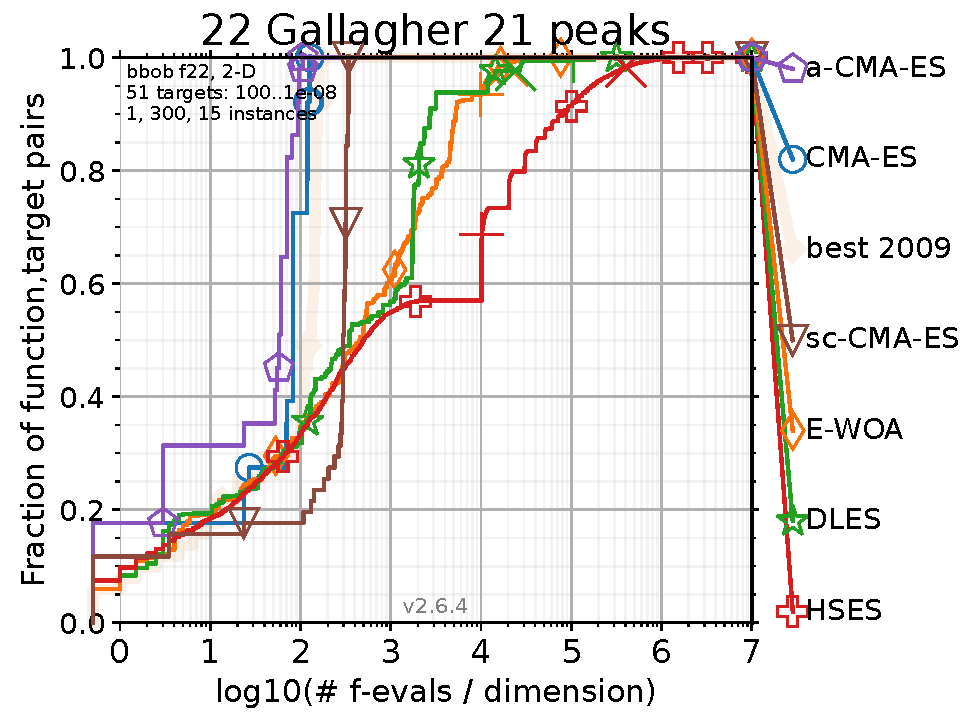
\includegraphics[width=\textwidth]{./bbob/pprldmany_f022_02D.pdf}
	\end{minipage}\hfill
	\begin{minipage}[b]{0.32\textwidth}
		\centering
		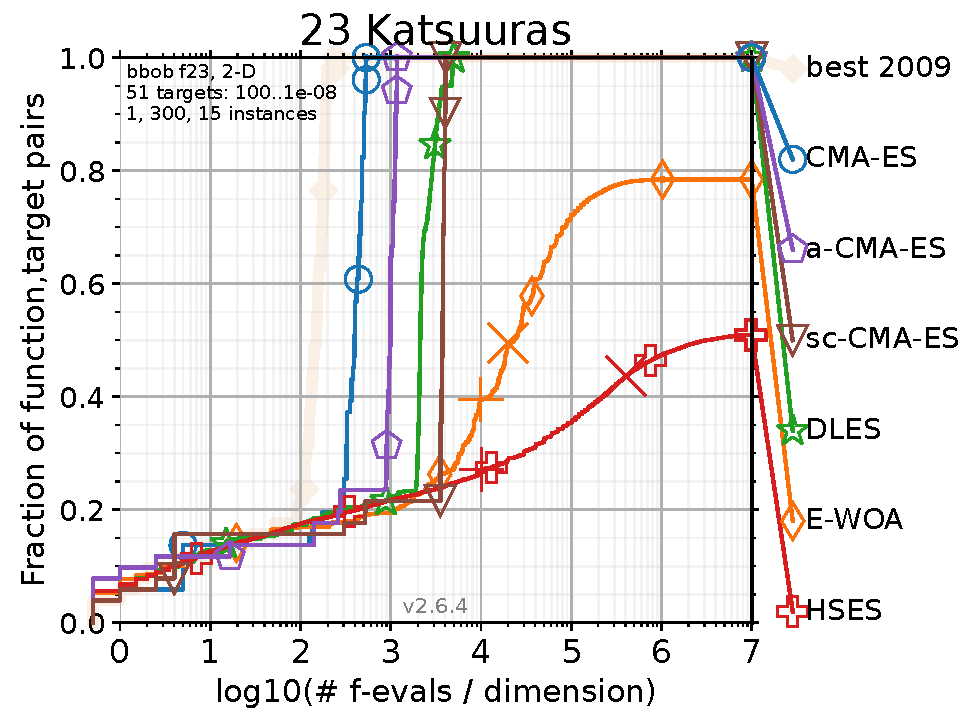
\includegraphics[width=\textwidth]{./bbob/pprldmany_f023_02D.pdf}
	\end{minipage}\hfill
	\begin{minipage}[b]{0.32\textwidth}
		\centering
		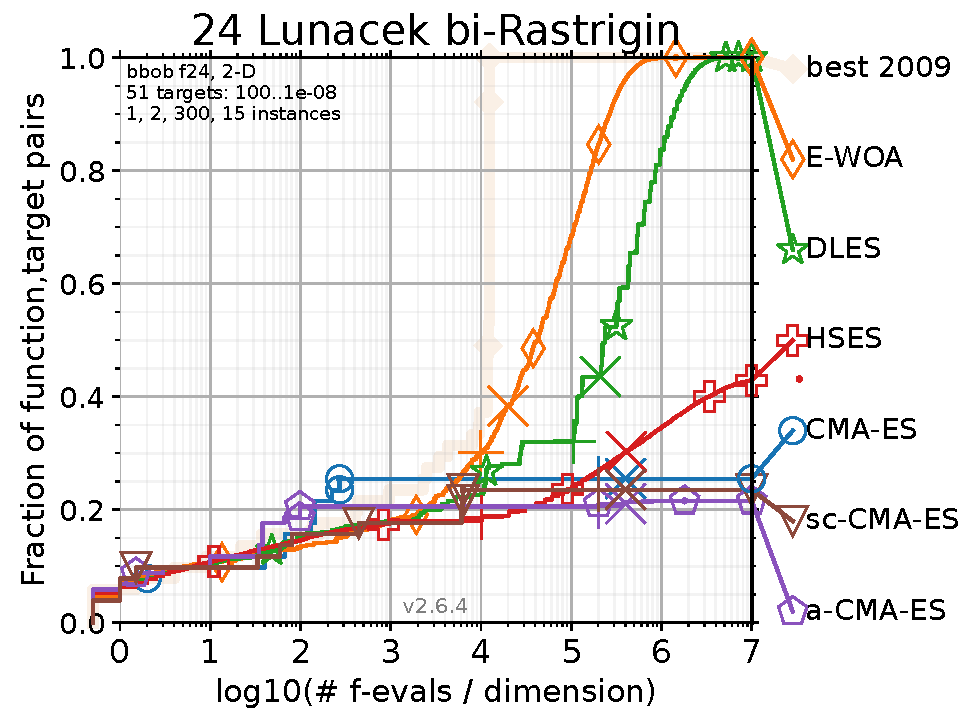
\includegraphics[width=\textwidth]{./bbob/pprldmany_f024_02D.pdf}
	\end{minipage}
	\caption{\textcolor{blue}{F22 to F24 in $D$ = 2.}}
\end{figure}


\begin{figure}[H]
	\centering
	\begin{minipage}[b]{0.32\textwidth}
		\centering
		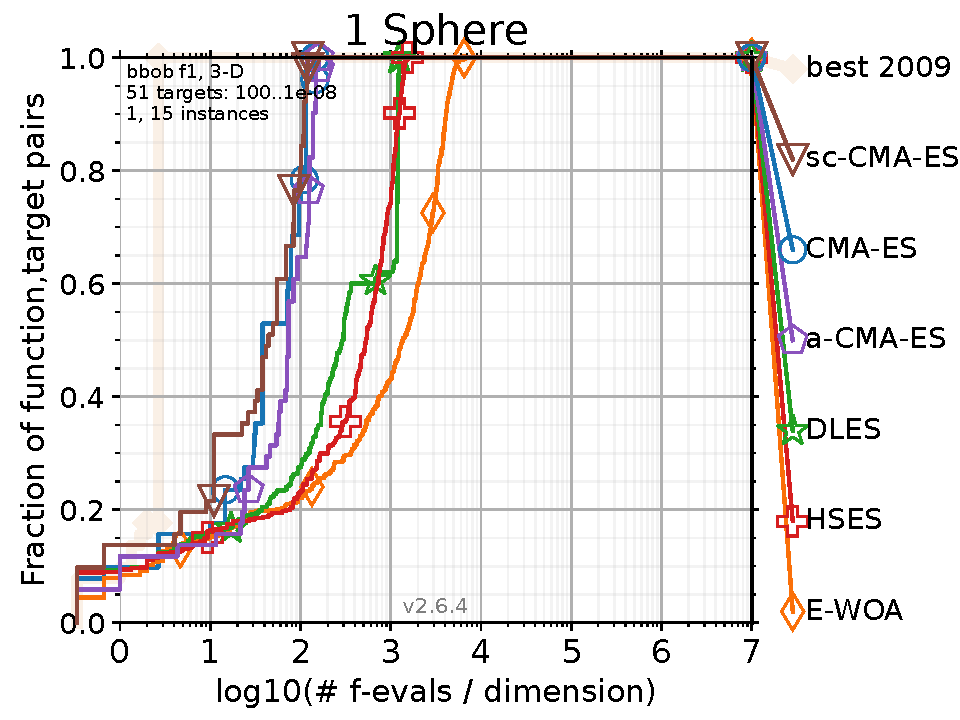
\includegraphics[width=\textwidth]{./bbob/pprldmany_f001_03D.pdf}
	\end{minipage}\hfill
	\begin{minipage}[b]{0.32\textwidth}
		\centering
		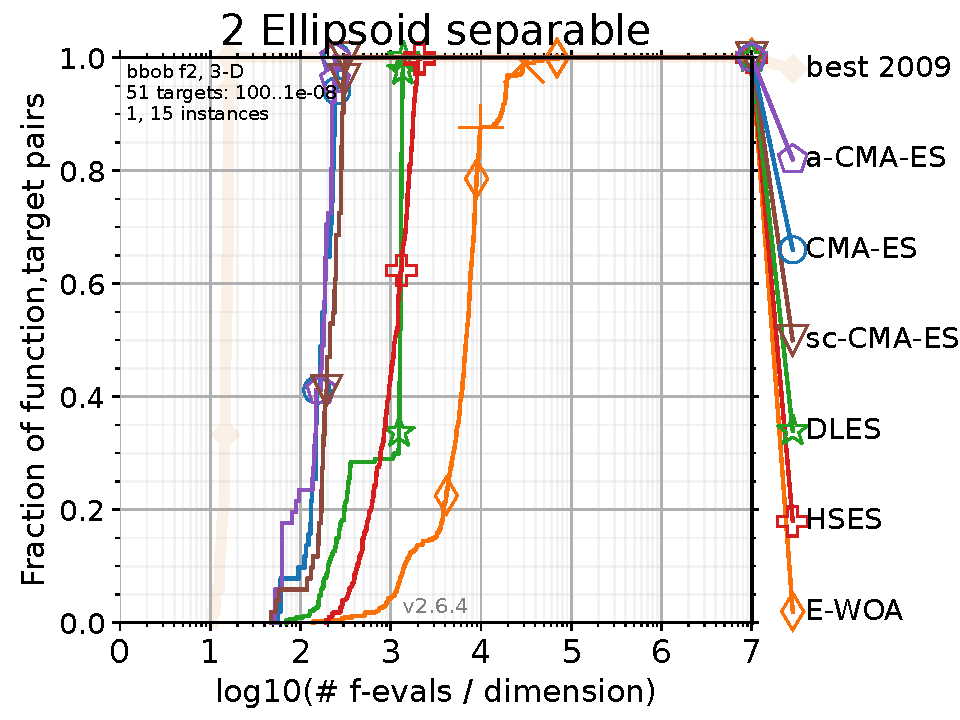
\includegraphics[width=\textwidth]{./bbob/pprldmany_f002_03D.pdf}
	\end{minipage}\hfill
	\begin{minipage}[b]{0.32\textwidth}
		\centering
		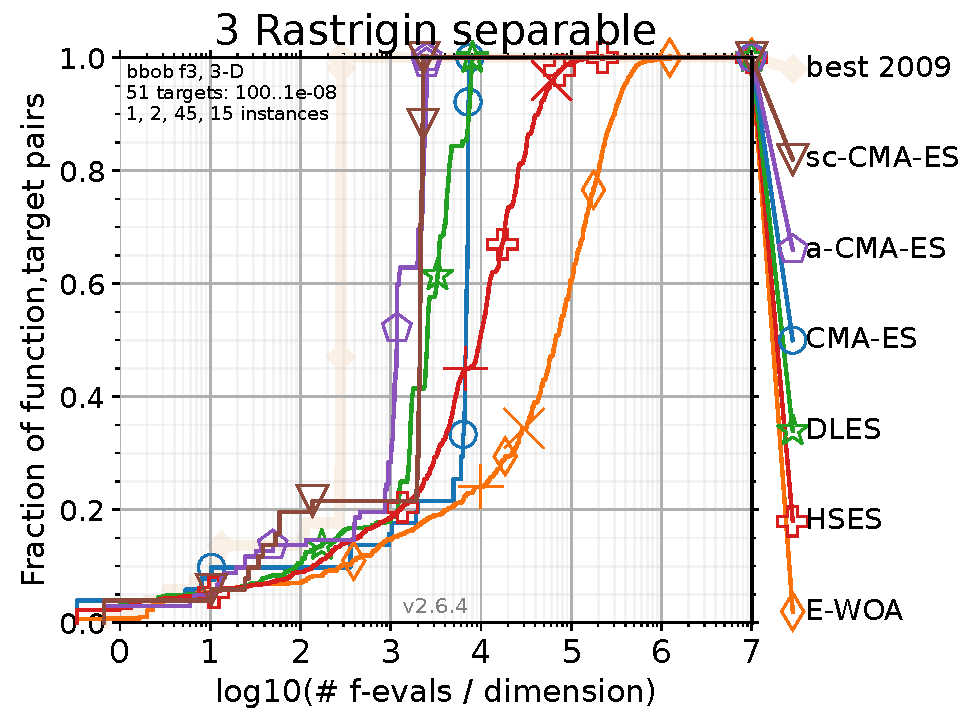
\includegraphics[width=\textwidth]{./bbob/pprldmany_f003_03D.pdf}
	\end{minipage}
	\caption{\textcolor{blue}{F1 to F3 in $D$ = 3.}}
\end{figure}

% 第二组图像
\begin{figure}[H]
	\centering
	\begin{minipage}[b]{0.32\textwidth}
		\centering
		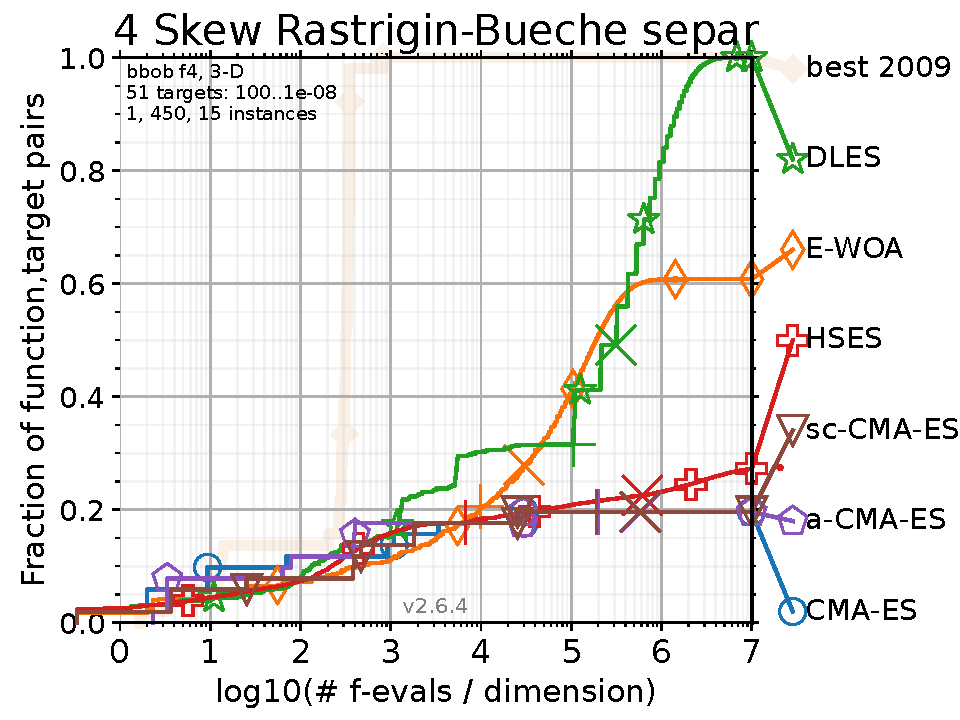
\includegraphics[width=\textwidth]{./bbob/pprldmany_f004_03D.pdf}
	\end{minipage}\hfill
	\begin{minipage}[b]{0.32\textwidth}
		\centering
		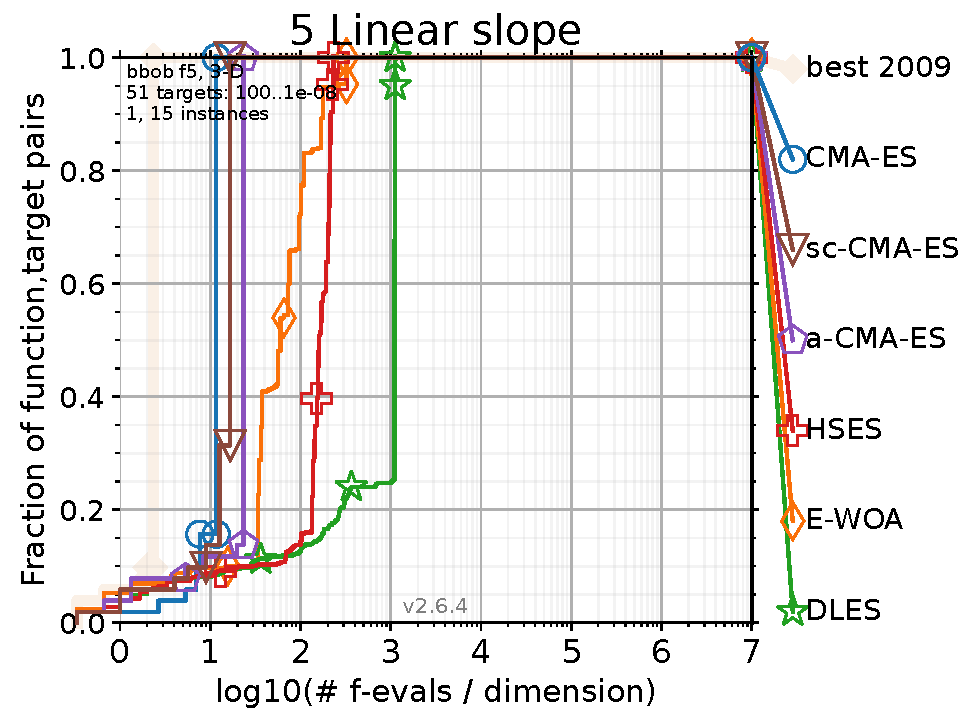
\includegraphics[width=\textwidth]{./bbob/pprldmany_f005_03D.pdf}
	\end{minipage}\hfill
	\begin{minipage}[b]{0.32\textwidth}
		\centering
		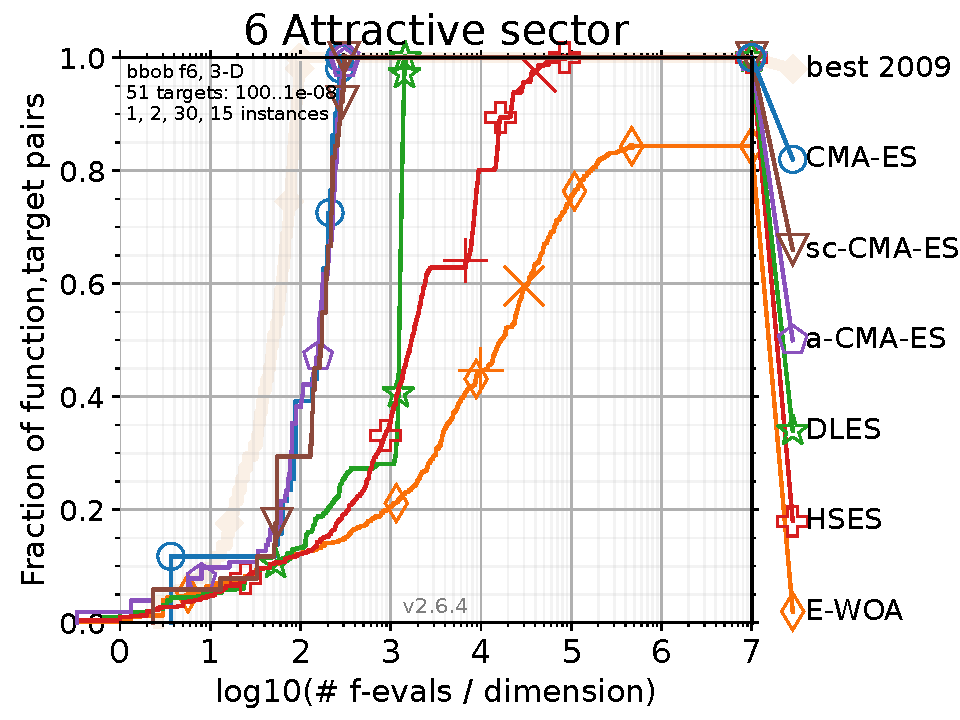
\includegraphics[width=\textwidth]{./bbob/pprldmany_f006_03D.pdf}
	\end{minipage}
	\caption{\textcolor{blue}{F4 to F6 in $D$ = 3.}}
\end{figure}

% 第三组图像
\begin{figure}[H]
	\centering
	\begin{minipage}[b]{0.32\textwidth}
		\centering
		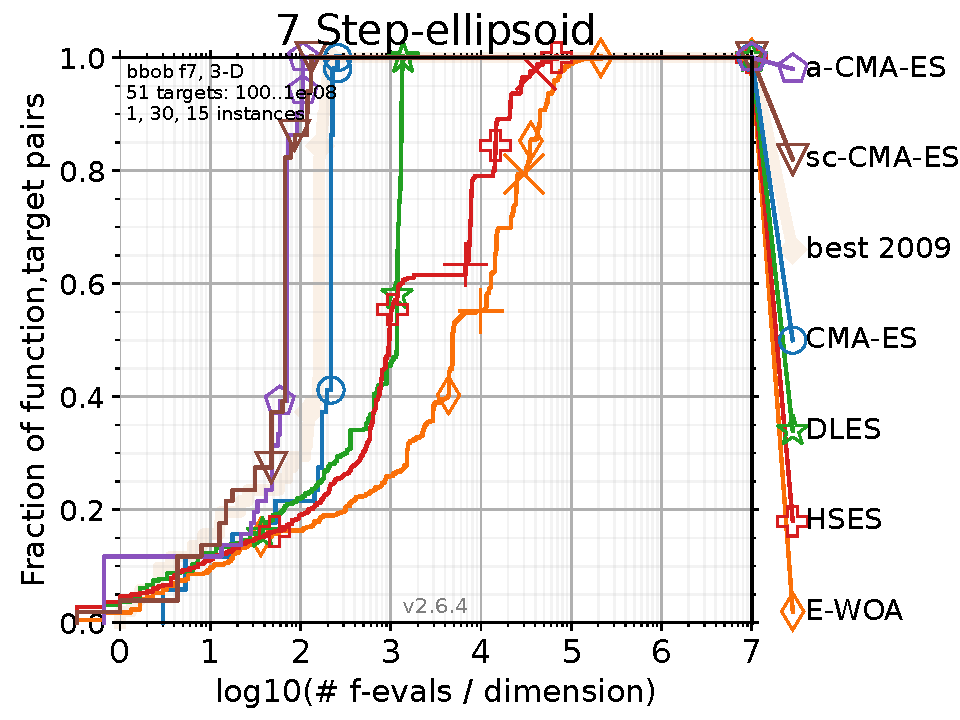
\includegraphics[width=\textwidth]{./bbob/pprldmany_f007_03D.pdf}
	\end{minipage}\hfill
	\begin{minipage}[b]{0.32\textwidth}
		\centering
		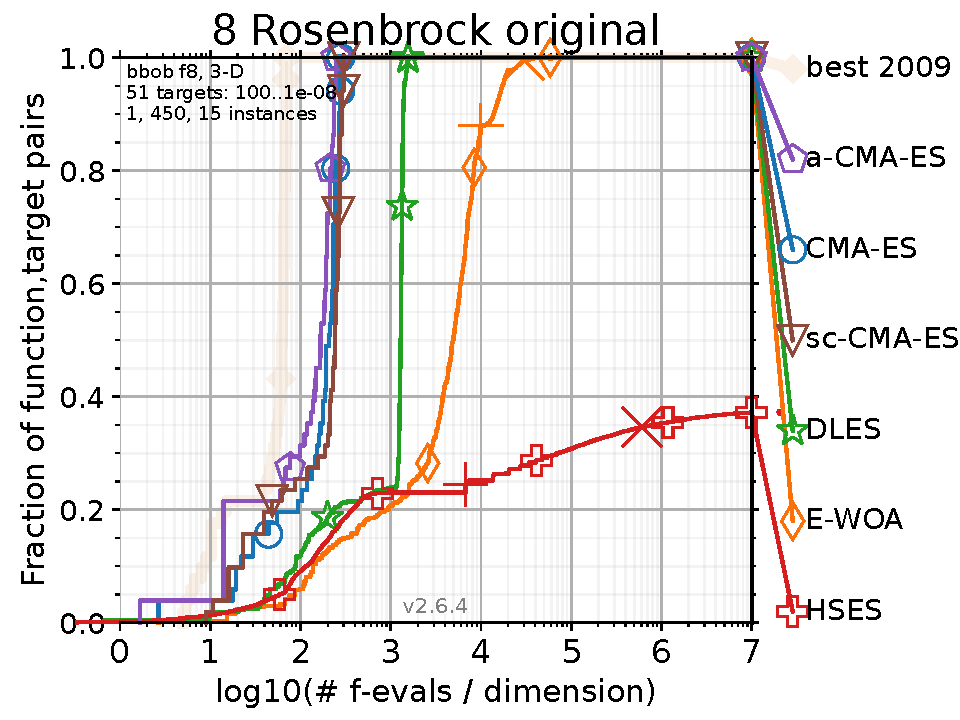
\includegraphics[width=\textwidth]{./bbob/pprldmany_f008_03D.pdf}
	\end{minipage}\hfill
	\begin{minipage}[b]{0.32\textwidth}
		\centering
		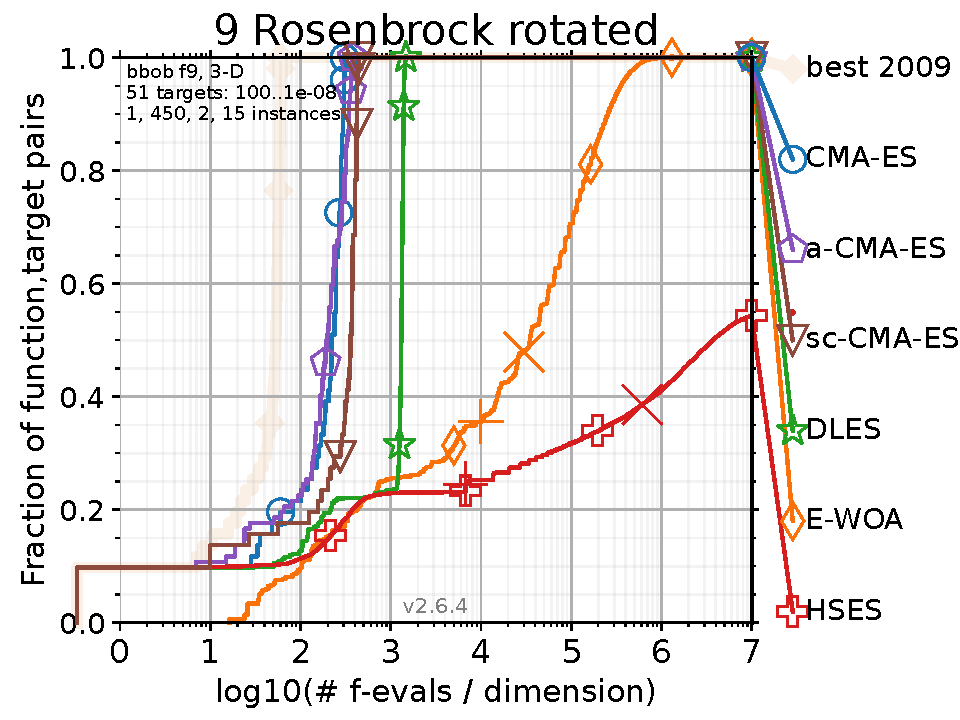
\includegraphics[width=\textwidth]{./bbob/pprldmany_f009_03D.pdf}
	\end{minipage}
	\caption{\textcolor{blue}{F7 to F9 in $D$ = 3.}}
\end{figure}

% 第四组图像
\begin{figure}[H]
	\centering
	\begin{minipage}[b]{0.32\textwidth}
		\centering
		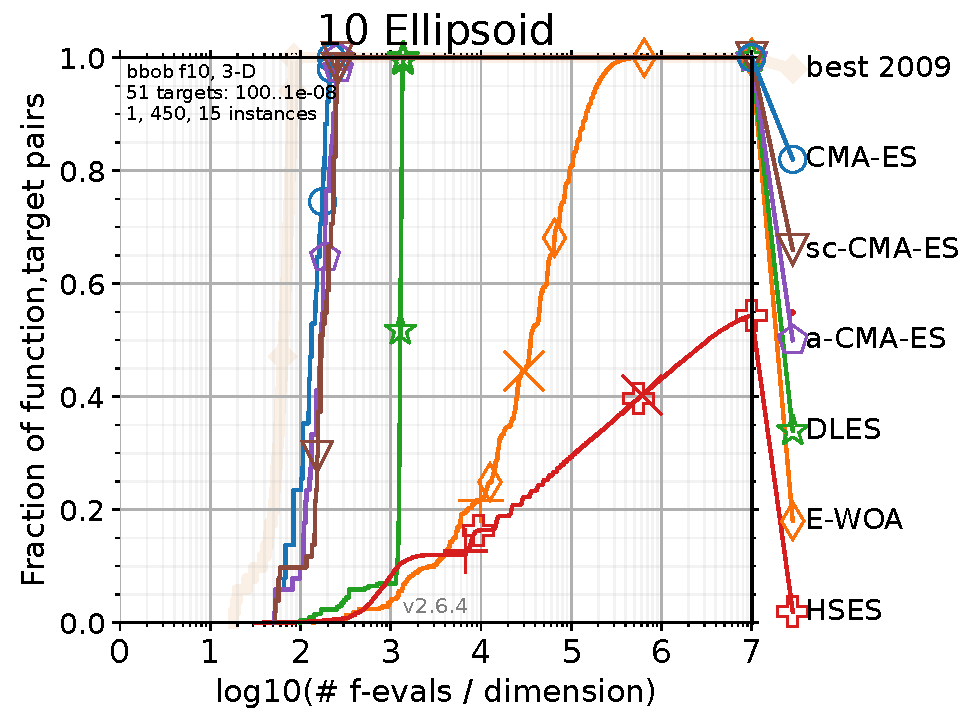
\includegraphics[width=\textwidth]{./bbob/pprldmany_f010_03D.pdf}
	\end{minipage}\hfill
	\begin{minipage}[b]{0.32\textwidth}
		\centering
		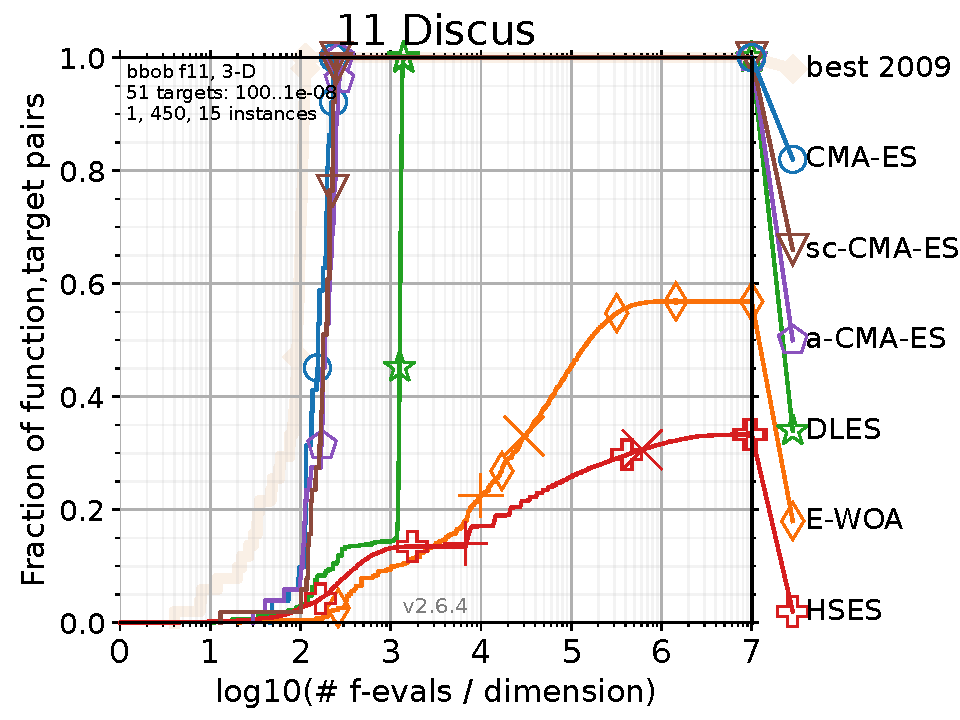
\includegraphics[width=\textwidth]{./bbob/pprldmany_f011_03D.pdf}
	\end{minipage}\hfill
	\begin{minipage}[b]{0.32\textwidth}
		\centering
		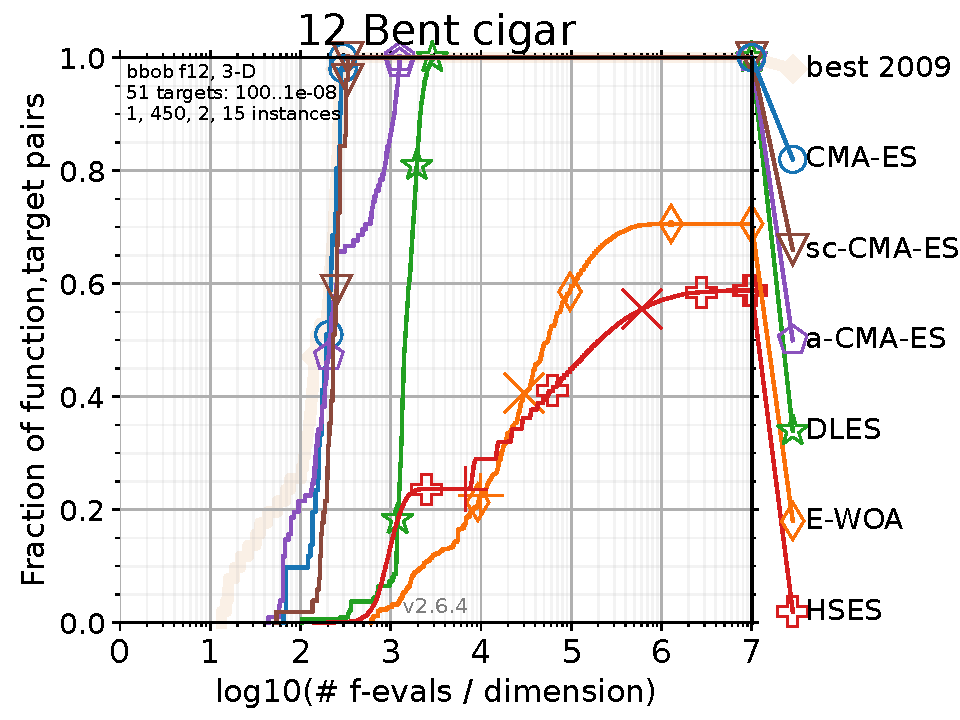
\includegraphics[width=\textwidth]{./bbob/pprldmany_f012_03D.pdf}
	\end{minipage}
	\caption{\textcolor{blue}{F10 to F12 in $D$ = 3.}}
\end{figure}

% 第五组图像
\begin{figure}[H]
	\centering
	\begin{minipage}[b]{0.32\textwidth}
		\centering
		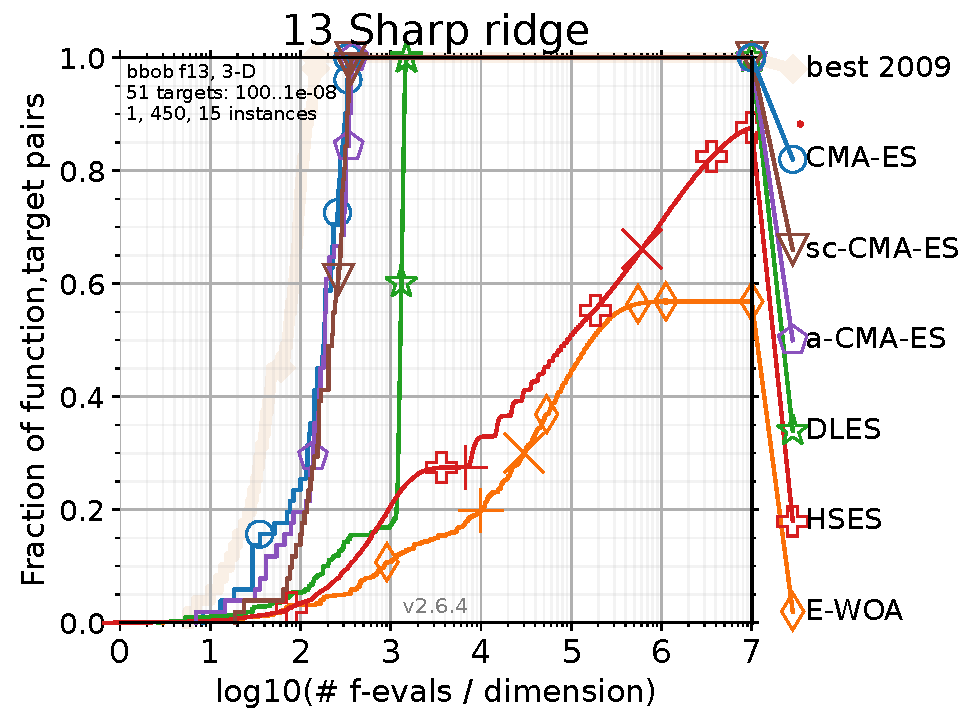
\includegraphics[width=\textwidth]{./bbob/pprldmany_f013_03D.pdf}
	\end{minipage}\hfill
	\begin{minipage}[b]{0.32\textwidth}
		\centering
		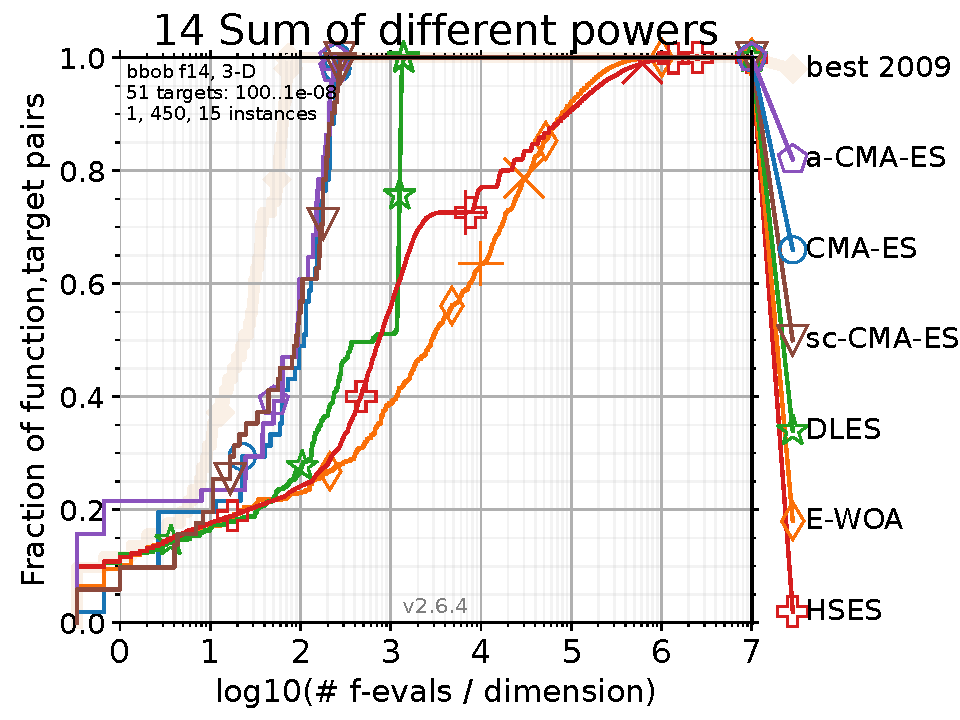
\includegraphics[width=\textwidth]{./bbob/pprldmany_f014_03D.pdf}
	\end{minipage}\hfill
	\begin{minipage}[b]{0.32\textwidth}
		\centering
		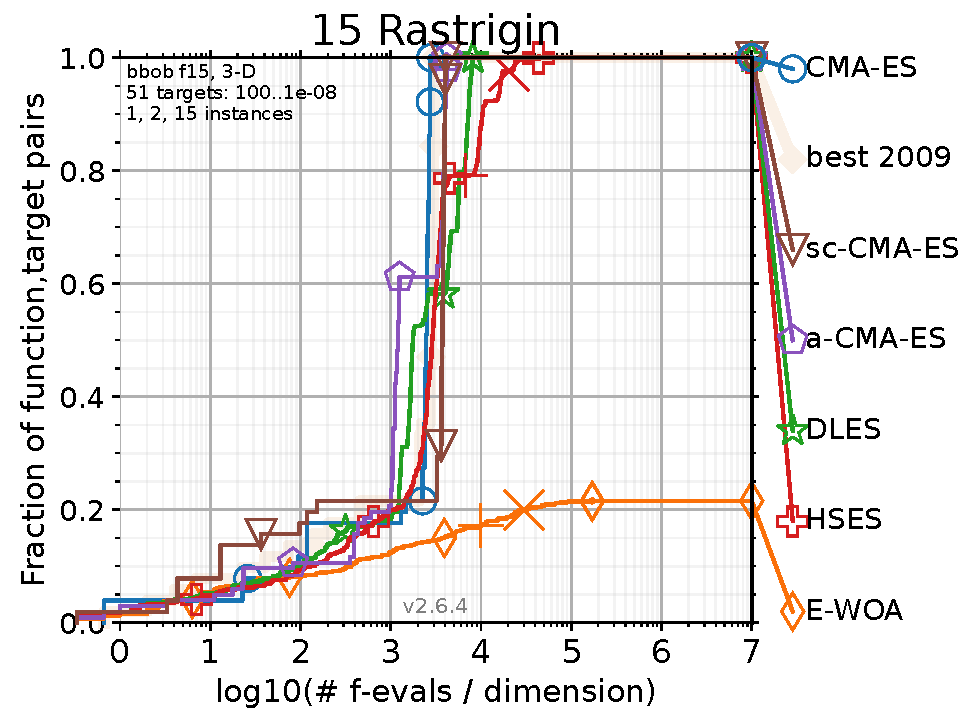
\includegraphics[width=\textwidth]{./bbob/pprldmany_f015_03D.pdf}
	\end{minipage}
	\caption{\textcolor{blue}{F13 to F15 in $D$ = 3.}}
\end{figure}

% 第六组图像
\begin{figure}[H]
	\centering
	\begin{minipage}[b]{0.32\textwidth}
		\centering
		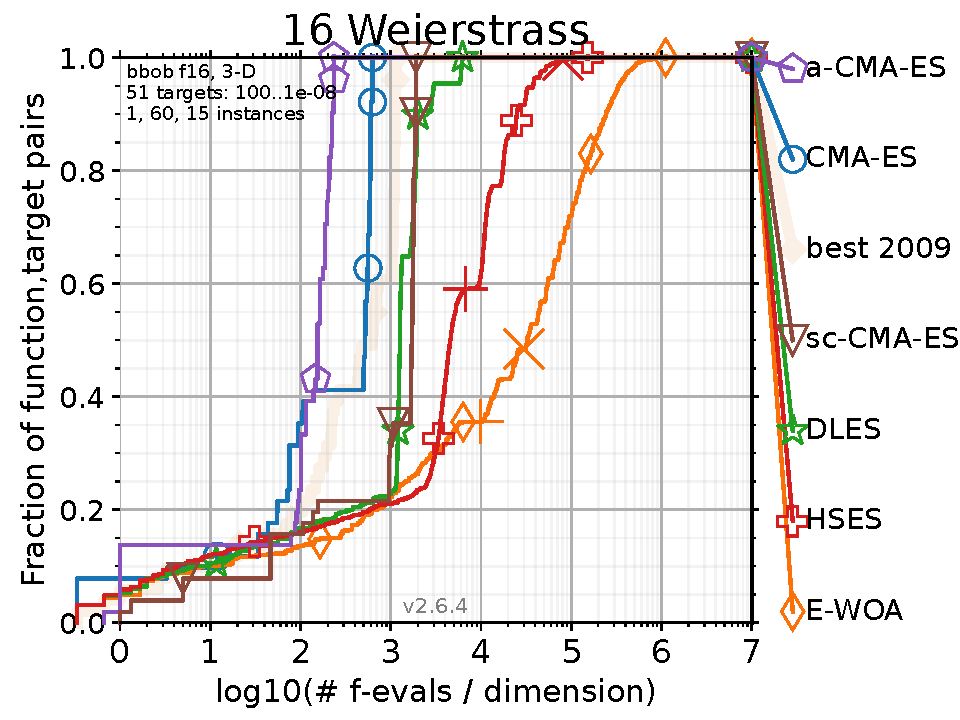
\includegraphics[width=\textwidth]{./bbob/pprldmany_f016_03D.pdf}
	\end{minipage}\hfill
	\begin{minipage}[b]{0.32\textwidth}
		\centering
		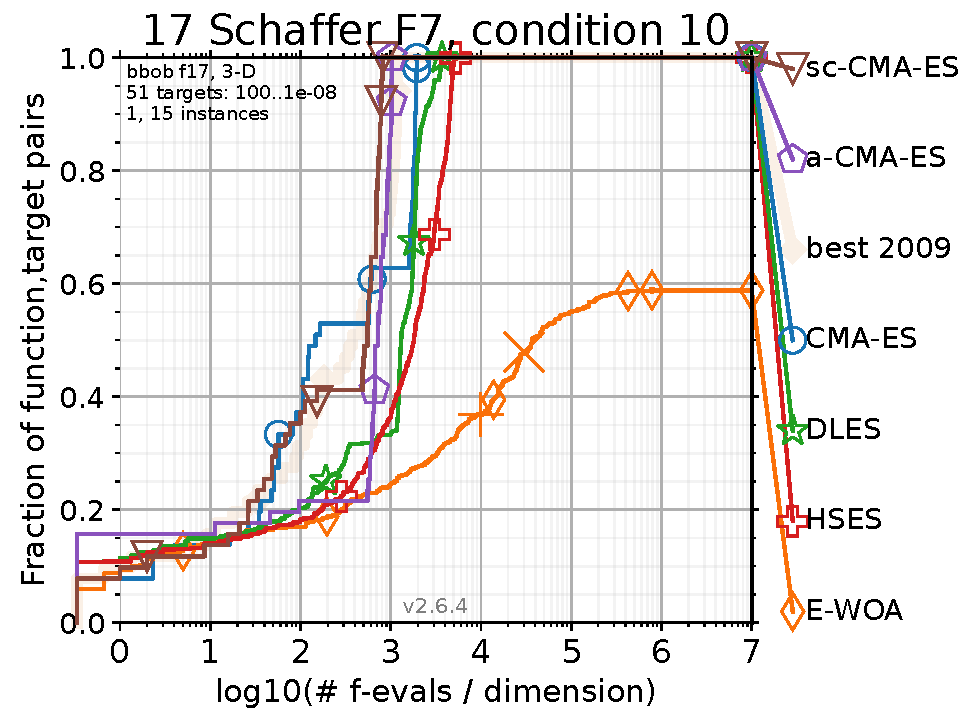
\includegraphics[width=\textwidth]{./bbob/pprldmany_f017_03D.pdf}
	\end{minipage}\hfill
	\begin{minipage}[b]{0.32\textwidth}
		\centering
		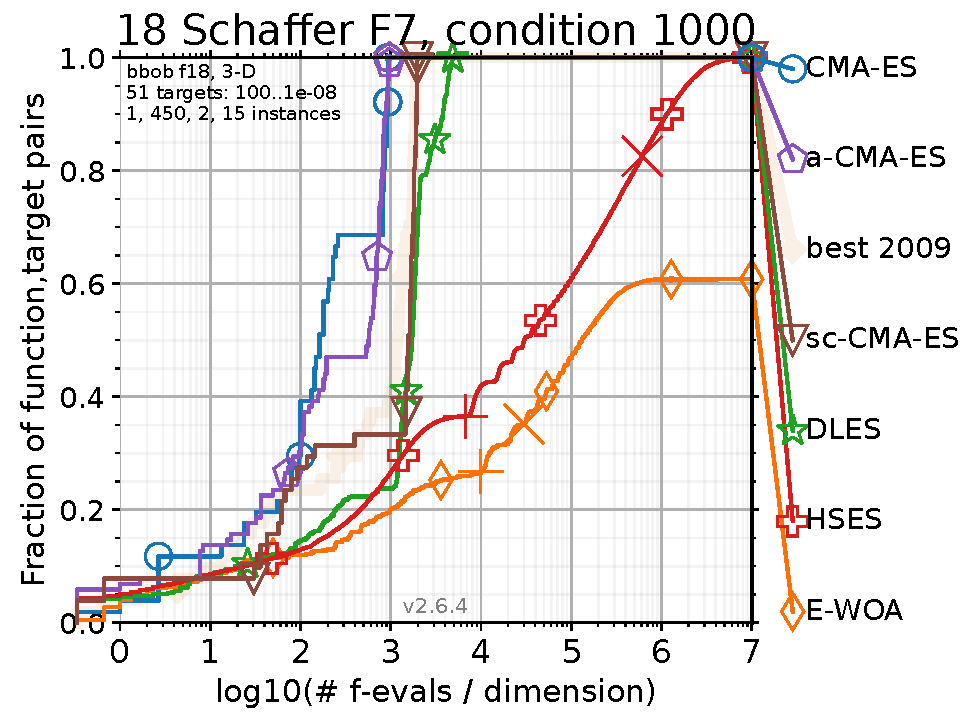
\includegraphics[width=\textwidth]{./bbob/pprldmany_f018_03D.pdf}
	\end{minipage}
	\caption{\textcolor{blue}{F16 to F18 in $D$ = 3.}}
\end{figure}

% 第七组图像
\begin{figure}[H]
	\centering
	\begin{minipage}[b]{0.32\textwidth}
		\centering
		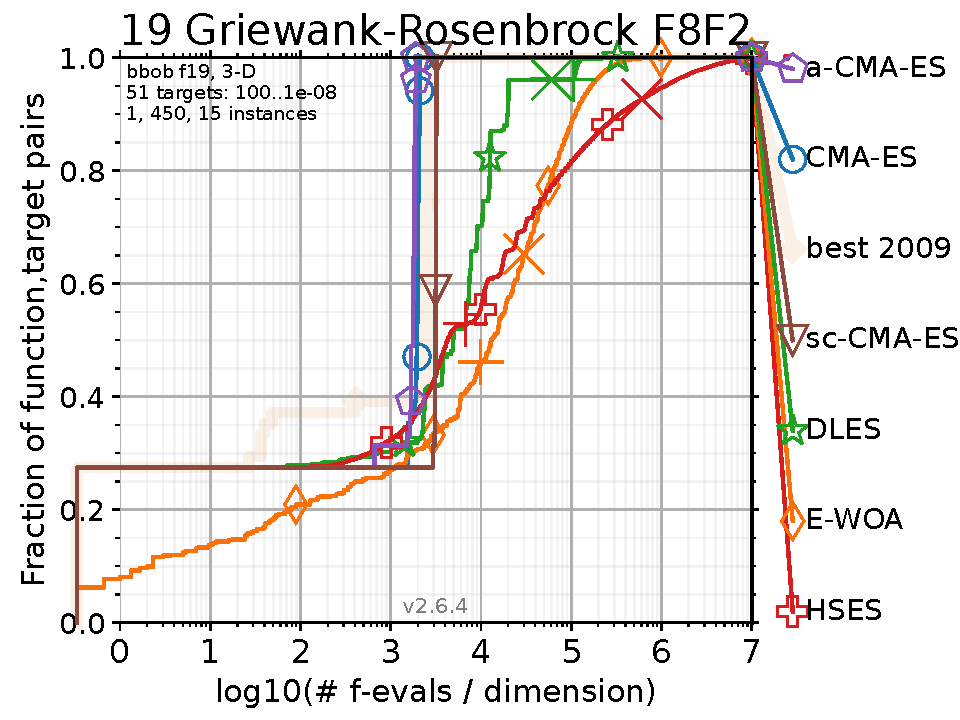
\includegraphics[width=\textwidth]{./bbob/pprldmany_f019_03D.pdf}
	\end{minipage}\hfill
	\begin{minipage}[b]{0.32\textwidth}
		\centering
		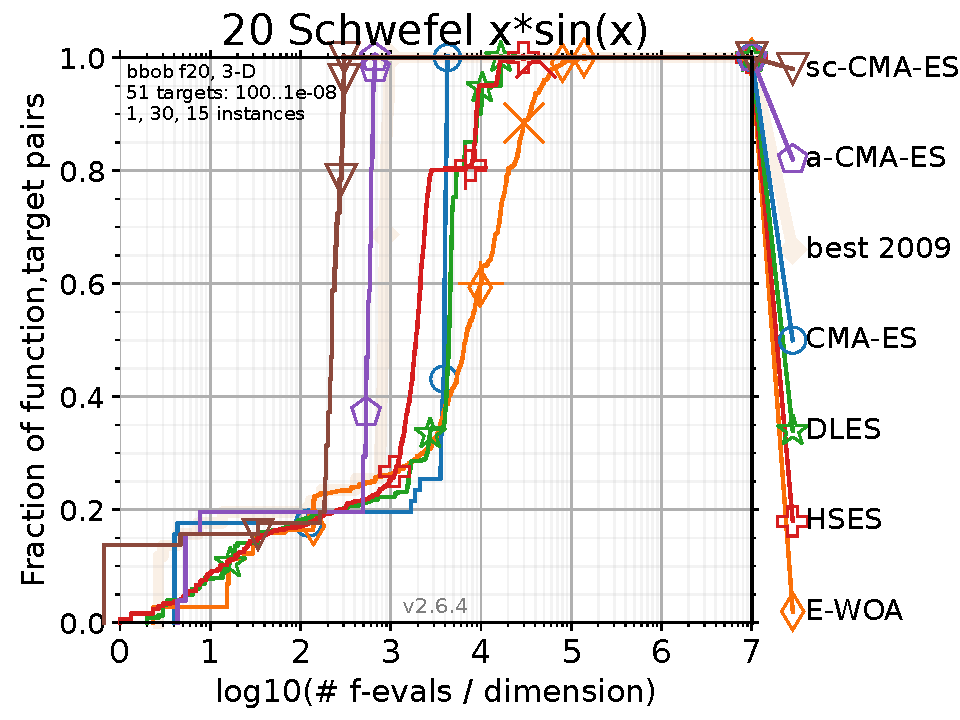
\includegraphics[width=\textwidth]{./bbob/pprldmany_f020_03D.pdf}
	\end{minipage}\hfill
	\begin{minipage}[b]{0.32\textwidth}
		\centering
		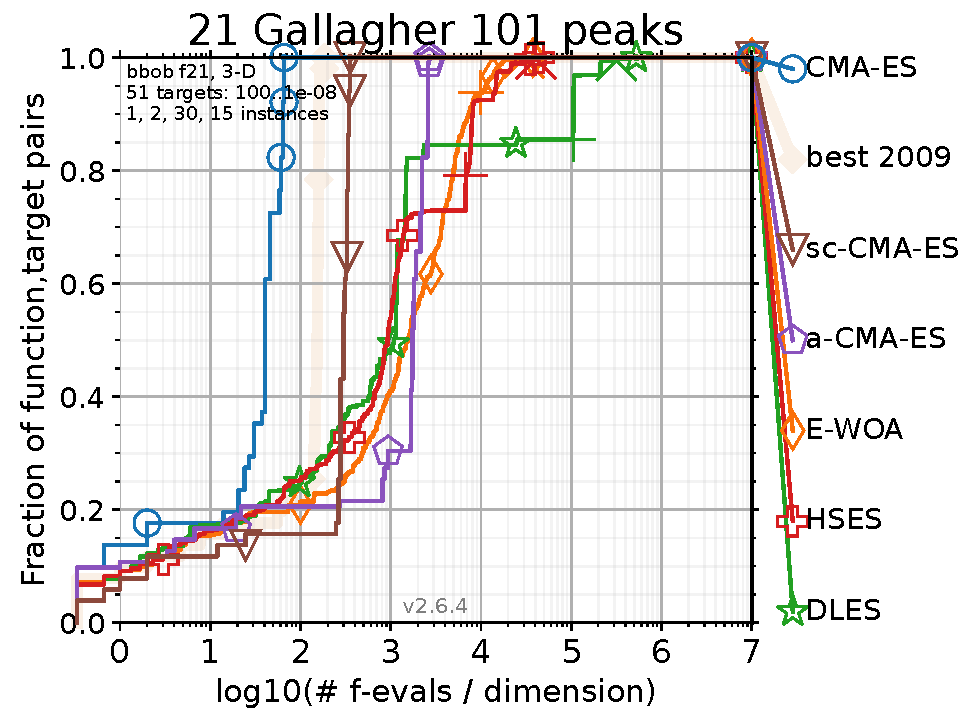
\includegraphics[width=\textwidth]{./bbob/pprldmany_f021_03D.pdf}
	\end{minipage}
	\caption{\textcolor{blue}{F19 to F21 in $D$ = 3.}}
\end{figure}

% 第八组图像
\begin{figure}[H]
	\centering
	\begin{minipage}[b]{0.32\textwidth}
		\centering
		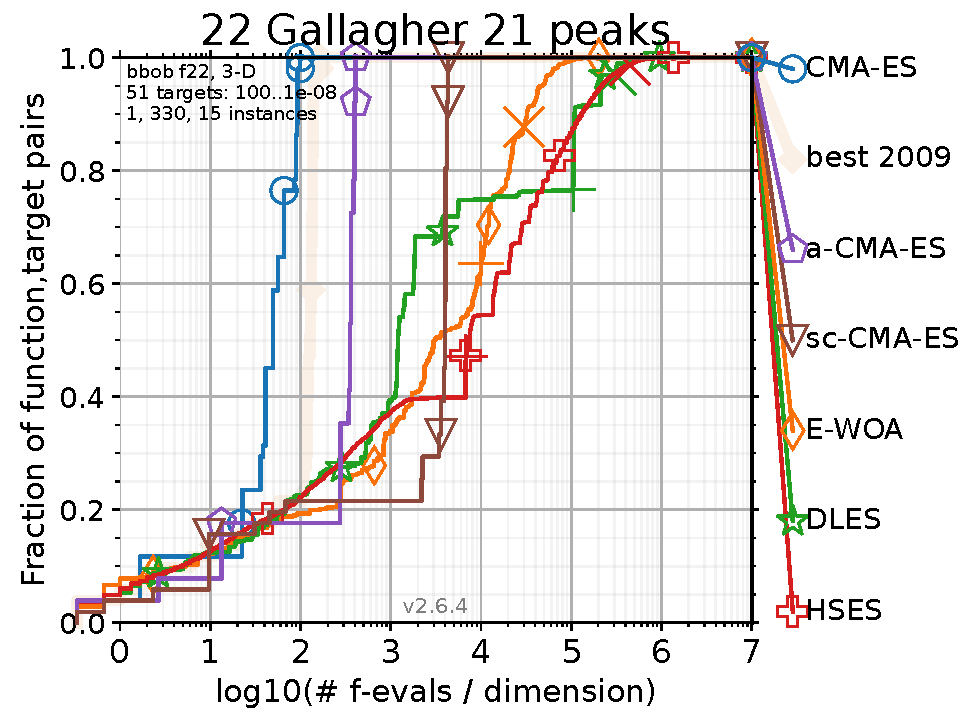
\includegraphics[width=\textwidth]{./bbob/pprldmany_f022_03D.pdf}
	\end{minipage}\hfill
	\begin{minipage}[b]{0.32\textwidth}
		\centering
		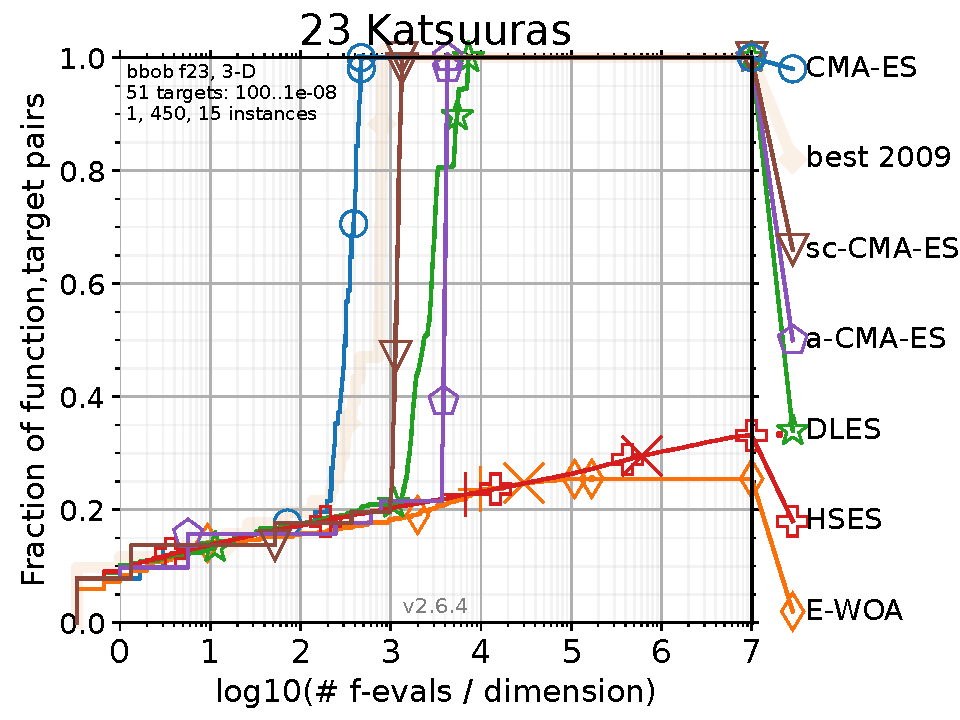
\includegraphics[width=\textwidth]{./bbob/pprldmany_f023_03D.pdf}
	\end{minipage}\hfill
	\begin{minipage}[b]{0.32\textwidth}
		\centering
		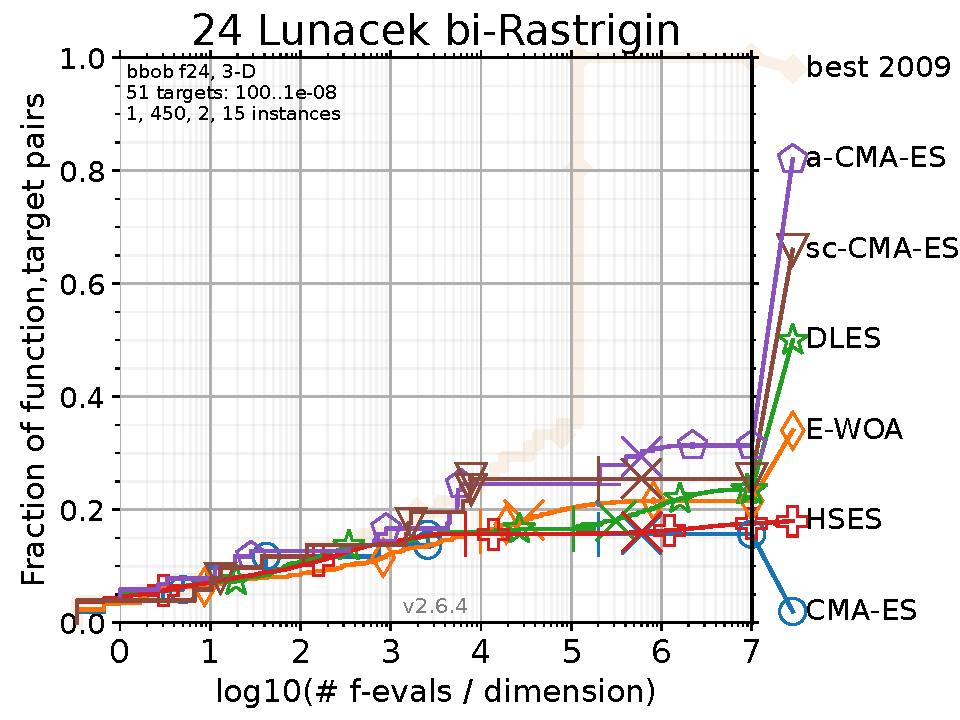
\includegraphics[width=\textwidth]{./bbob/pprldmany_f024_03D.pdf}
	\end{minipage}
	\caption{\textcolor{blue}{F22 to F24 in $D$ = 3.}}
\end{figure}

\begin{figure}[H]
	\centering
	\begin{minipage}[b]{0.32\textwidth}
		\centering
		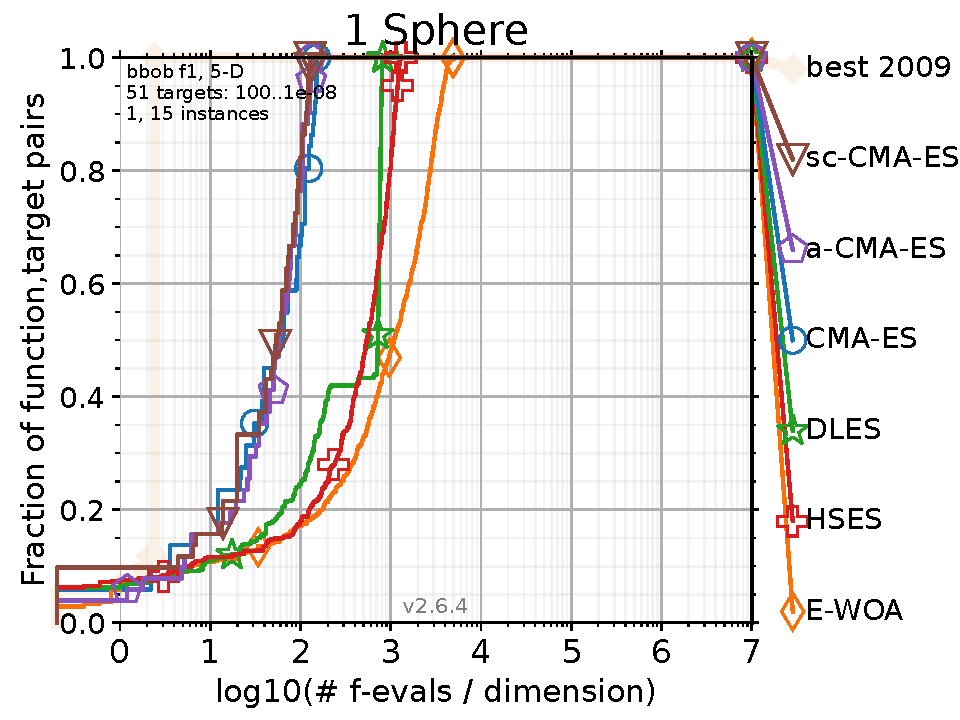
\includegraphics[width=\textwidth]{./bbob/pprldmany_f001_05D.pdf}
	\end{minipage}\hfill
	\begin{minipage}[b]{0.32\textwidth}
		\centering
		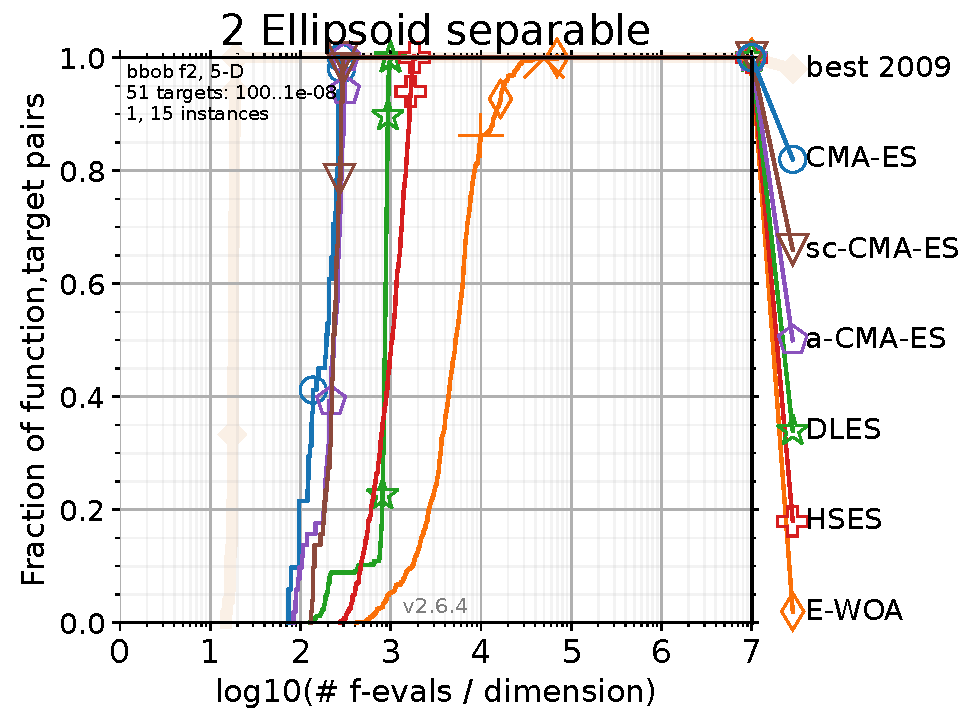
\includegraphics[width=\textwidth]{./bbob/pprldmany_f002_05D.pdf}
	\end{minipage}\hfill
	\begin{minipage}[b]{0.32\textwidth}
		\centering
		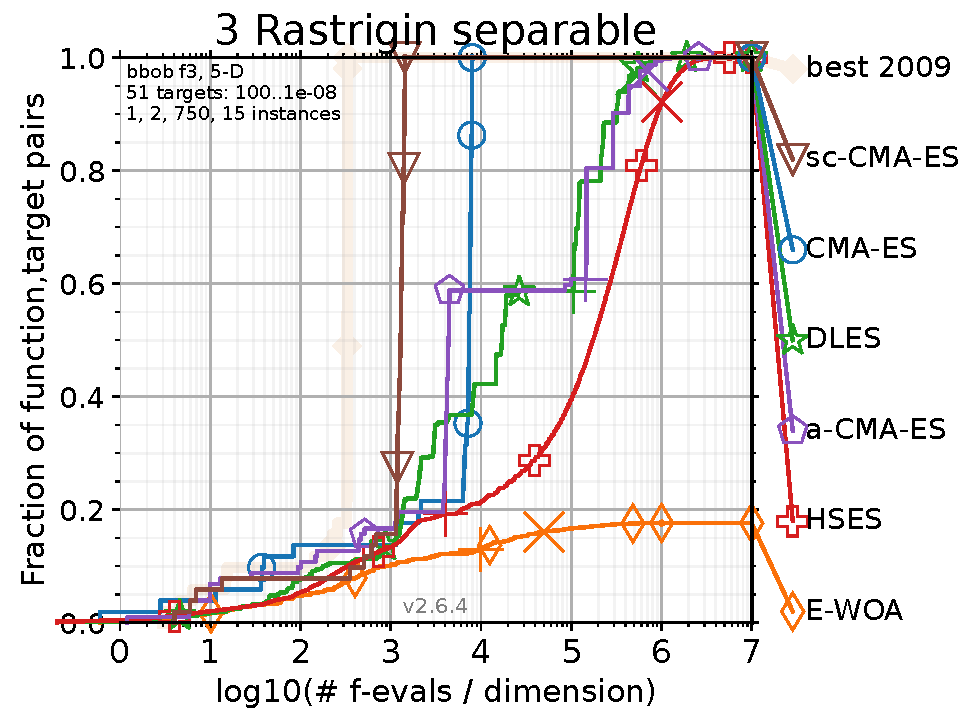
\includegraphics[width=\textwidth]{./bbob/pprldmany_f003_05D.pdf}
	\end{minipage}
	\caption{\textcolor{blue}{F1 to F3 in $D$ = 5.}}
\end{figure}

% 第二组图像
\begin{figure}[H]
	\centering
	\begin{minipage}[b]{0.32\textwidth}
		\centering
		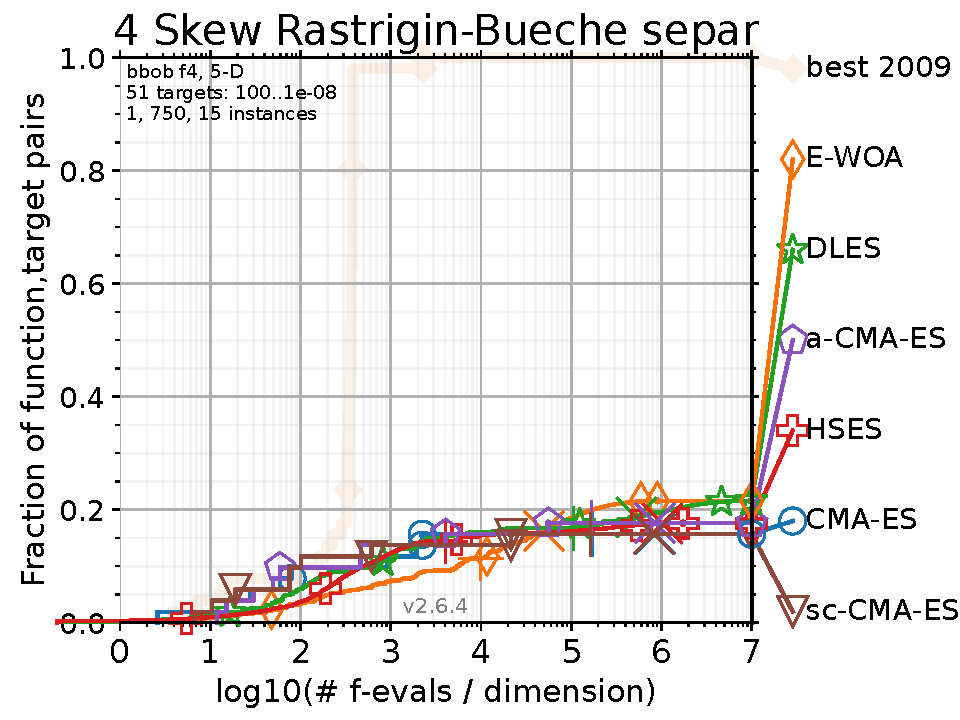
\includegraphics[width=\textwidth]{./bbob/pprldmany_f004_05D.pdf}
	\end{minipage}\hfill
	\begin{minipage}[b]{0.32\textwidth}
		\centering
		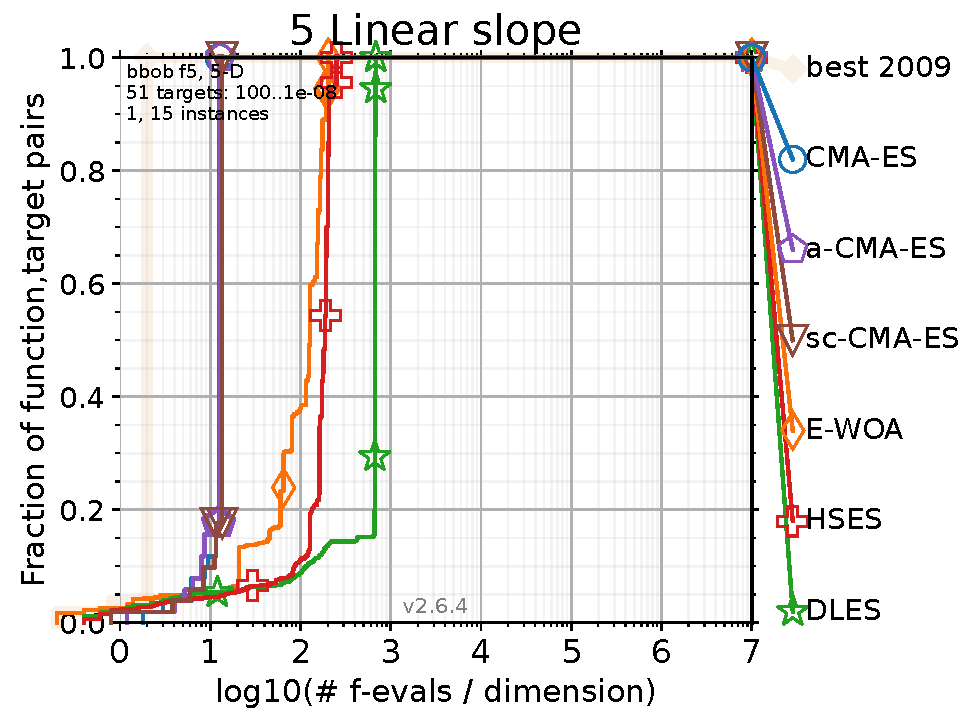
\includegraphics[width=\textwidth]{./bbob/pprldmany_f005_05D.pdf}
	\end{minipage}\hfill
	\begin{minipage}[b]{0.32\textwidth}
		\centering
		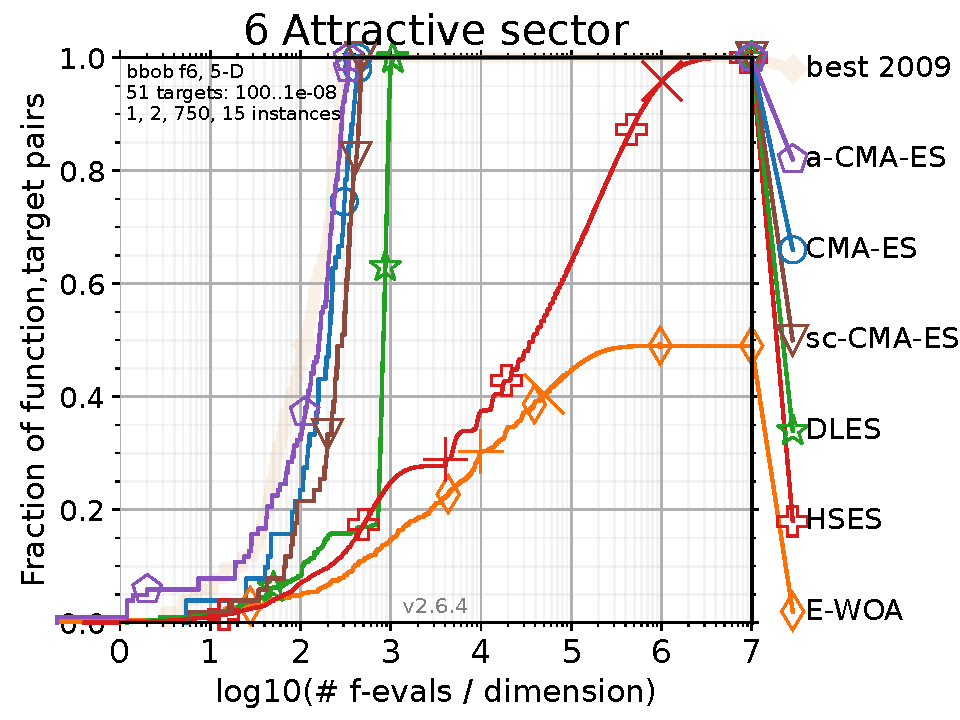
\includegraphics[width=\textwidth]{./bbob/pprldmany_f006_05D.pdf}
	\end{minipage}
	\caption{\textcolor{blue}{F4 to F6 in $D$ = 5.}}
\end{figure}

% 第三组图像
\begin{figure}[H]
	\centering
	\begin{minipage}[b]{0.32\textwidth}
		\centering
		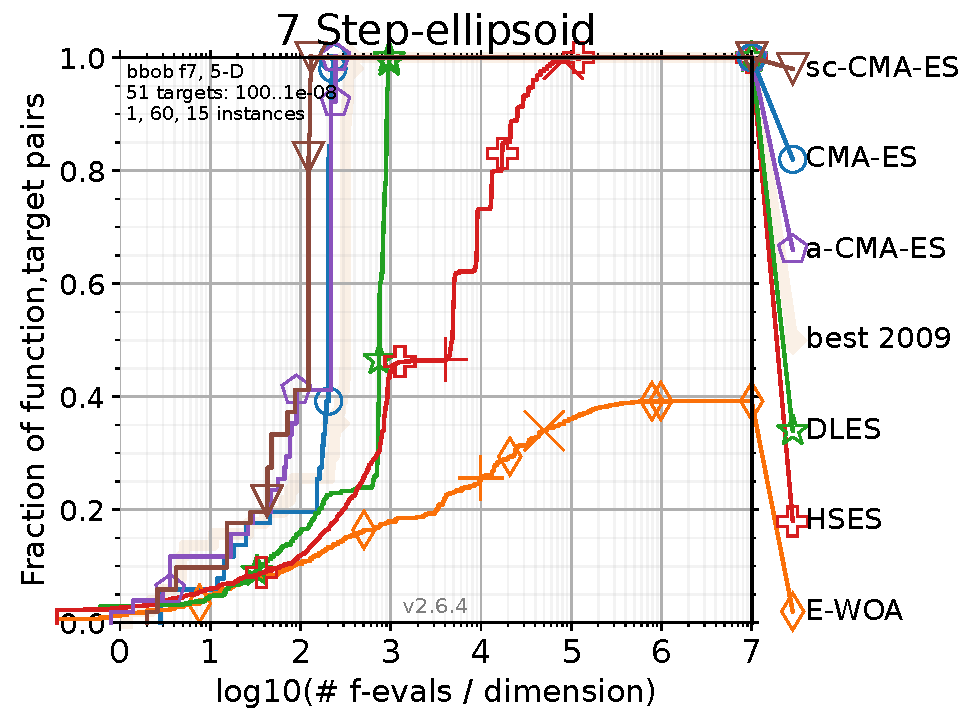
\includegraphics[width=\textwidth]{./bbob/pprldmany_f007_05D.pdf}
	\end{minipage}\hfill
	\begin{minipage}[b]{0.32\textwidth}
		\centering
		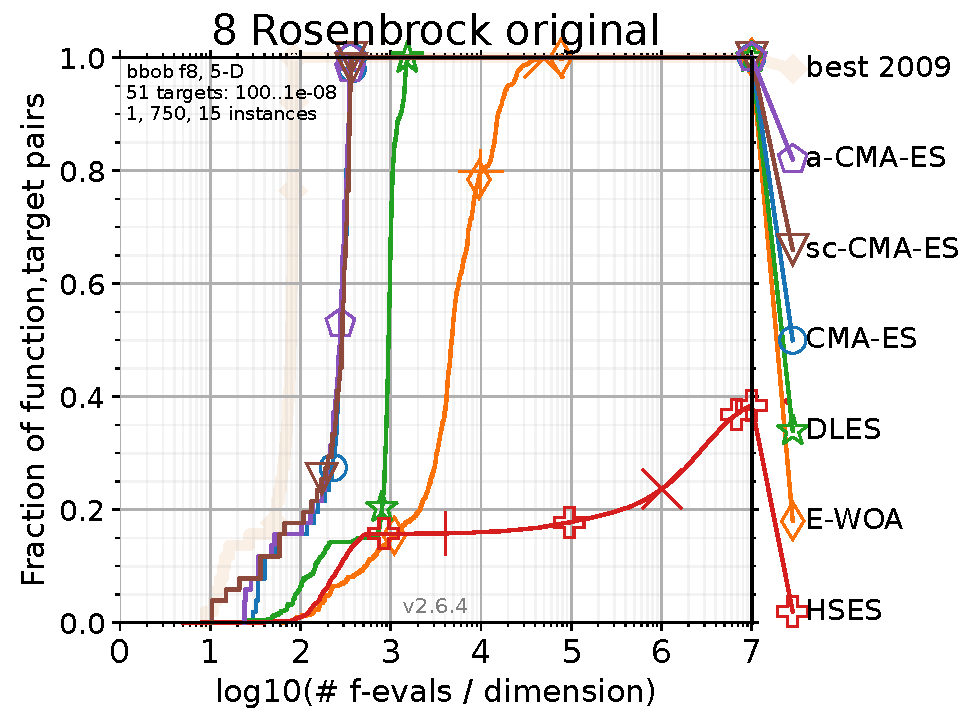
\includegraphics[width=\textwidth]{./bbob/pprldmany_f008_05D.pdf}
	\end{minipage}\hfill
	\begin{minipage}[b]{0.32\textwidth}
		\centering
		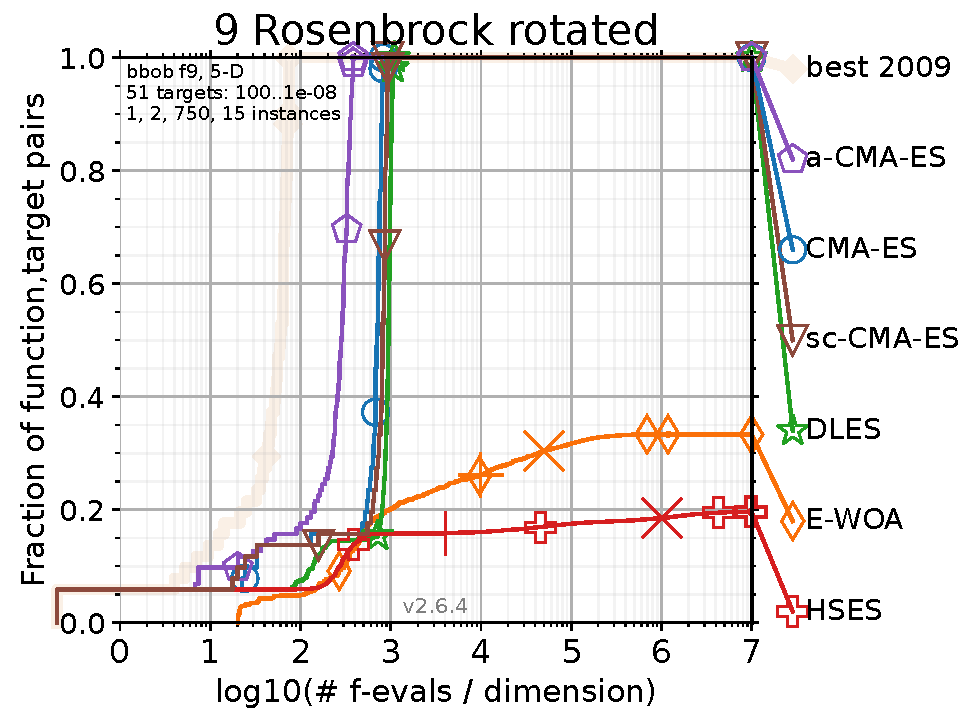
\includegraphics[width=\textwidth]{./bbob/pprldmany_f009_05D.pdf}
	\end{minipage}
	\caption{\textcolor{blue}{F7 to F9 in $D$ = 5.}}
\end{figure}

% 第四组图像
\begin{figure}[H]
	\centering
	\begin{minipage}[b]{0.32\textwidth}
		\centering
		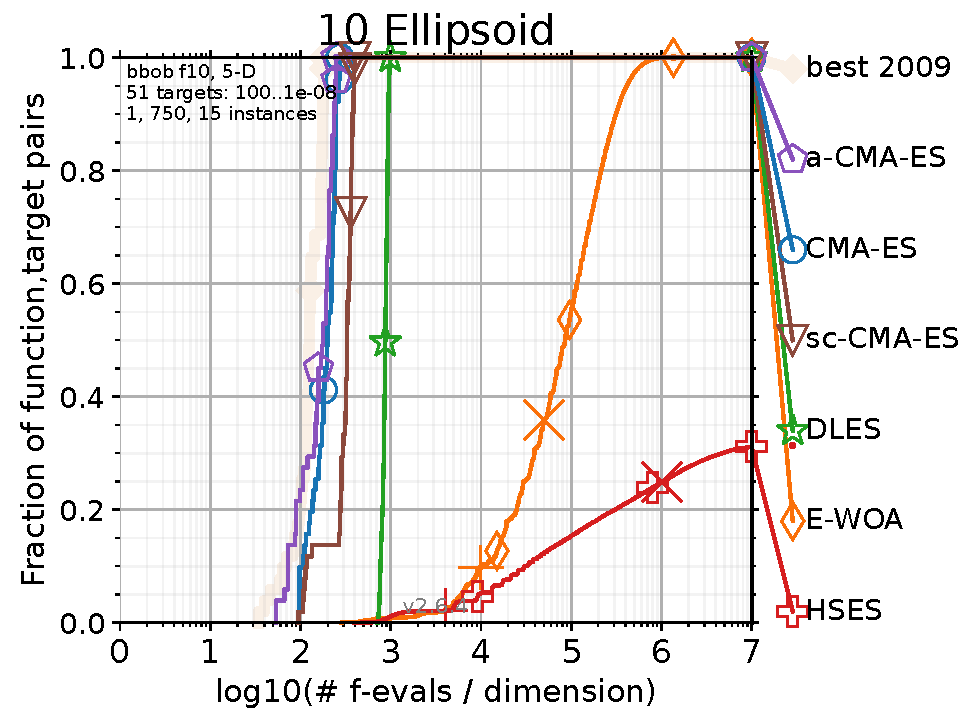
\includegraphics[width=\textwidth]{./bbob/pprldmany_f010_05D.pdf}
	\end{minipage}\hfill
	\begin{minipage}[b]{0.32\textwidth}
		\centering
		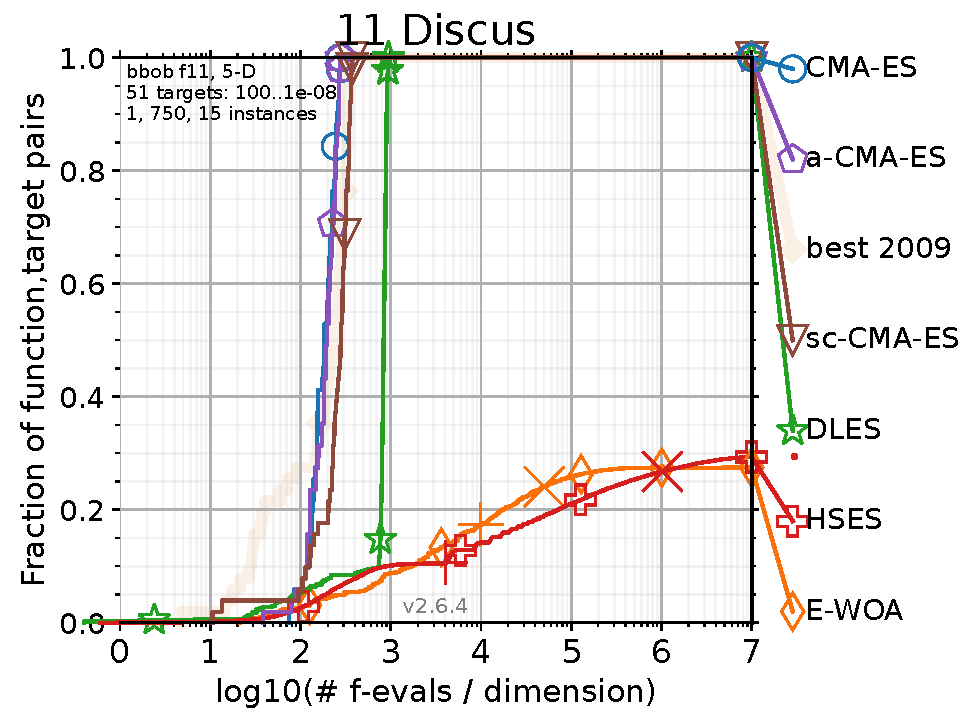
\includegraphics[width=\textwidth]{./bbob/pprldmany_f011_05D.pdf}
	\end{minipage}\hfill
	\begin{minipage}[b]{0.32\textwidth}
		\centering
		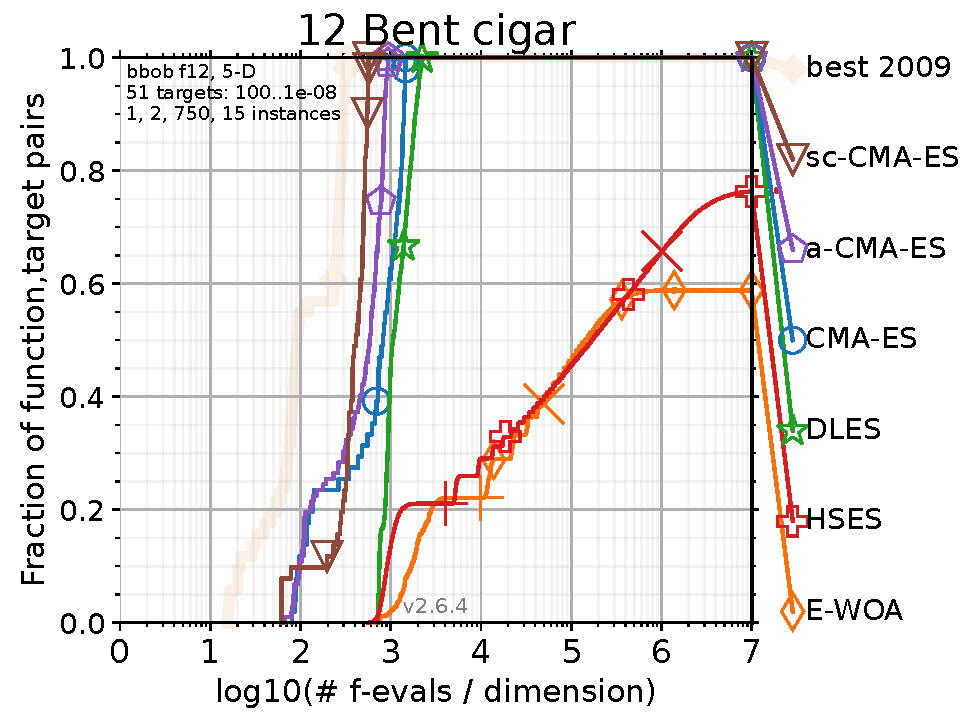
\includegraphics[width=\textwidth]{./bbob/pprldmany_f012_05D.pdf}
	\end{minipage}
	\caption{\textcolor{blue}{F10 to F12 in $D$ = 5.}}
\end{figure}

% 第五组图像
\begin{figure}[H]
	\centering
	\begin{minipage}[b]{0.32\textwidth}
		\centering
		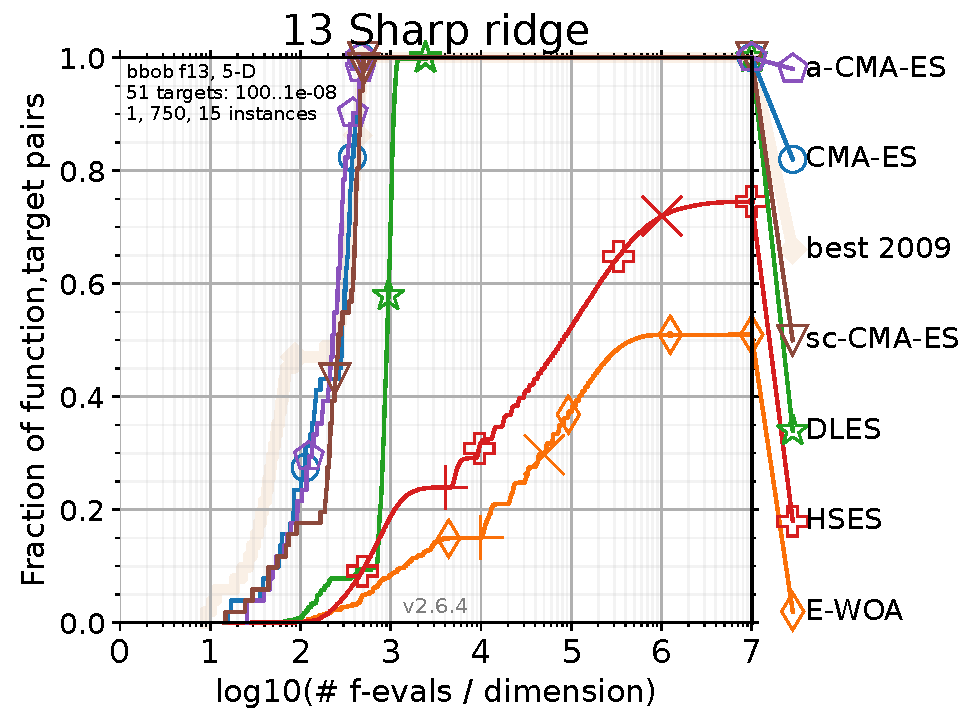
\includegraphics[width=\textwidth]{./bbob/pprldmany_f013_05D.pdf}
	\end{minipage}\hfill
	\begin{minipage}[b]{0.32\textwidth}
		\centering
		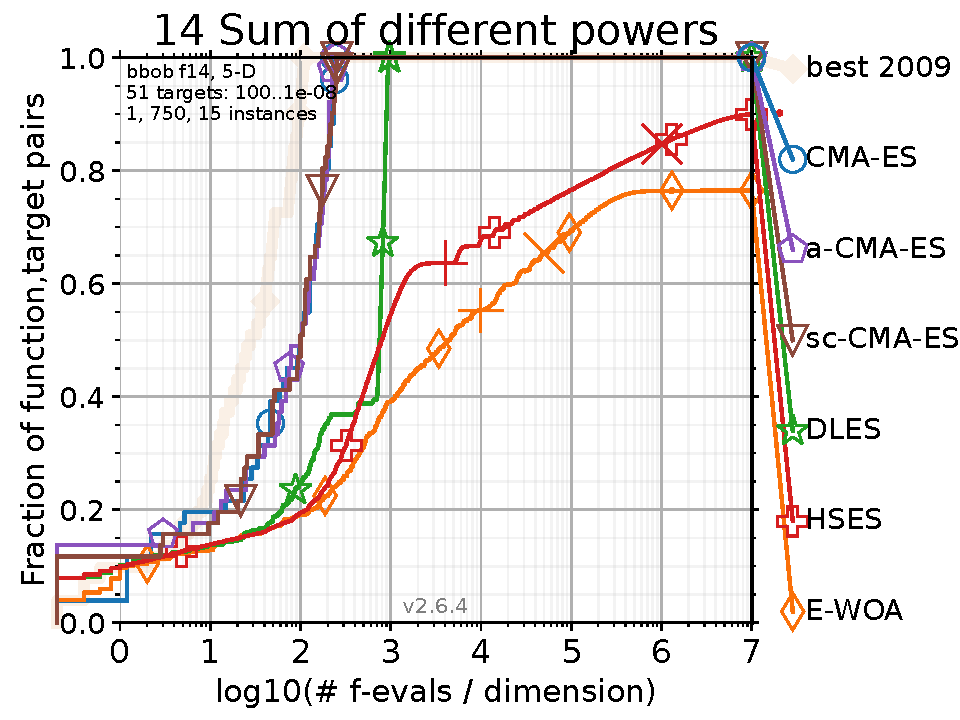
\includegraphics[width=\textwidth]{./bbob/pprldmany_f014_05D.pdf}
	\end{minipage}\hfill
	\begin{minipage}[b]{0.32\textwidth}
		\centering
		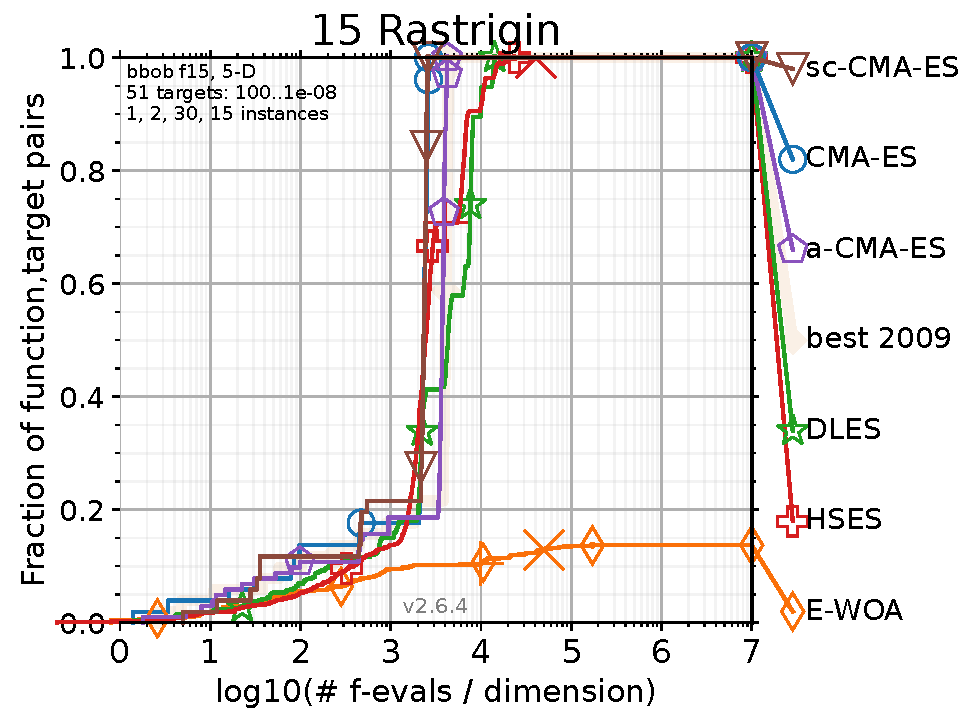
\includegraphics[width=\textwidth]{./bbob/pprldmany_f015_05D.pdf}
	\end{minipage}
	\caption{\textcolor{blue}{F13 to F15 in $D$ = 5.}}
\end{figure}

% 第六组图像
\begin{figure}[H]
	\centering
	\begin{minipage}[b]{0.32\textwidth}
		\centering
		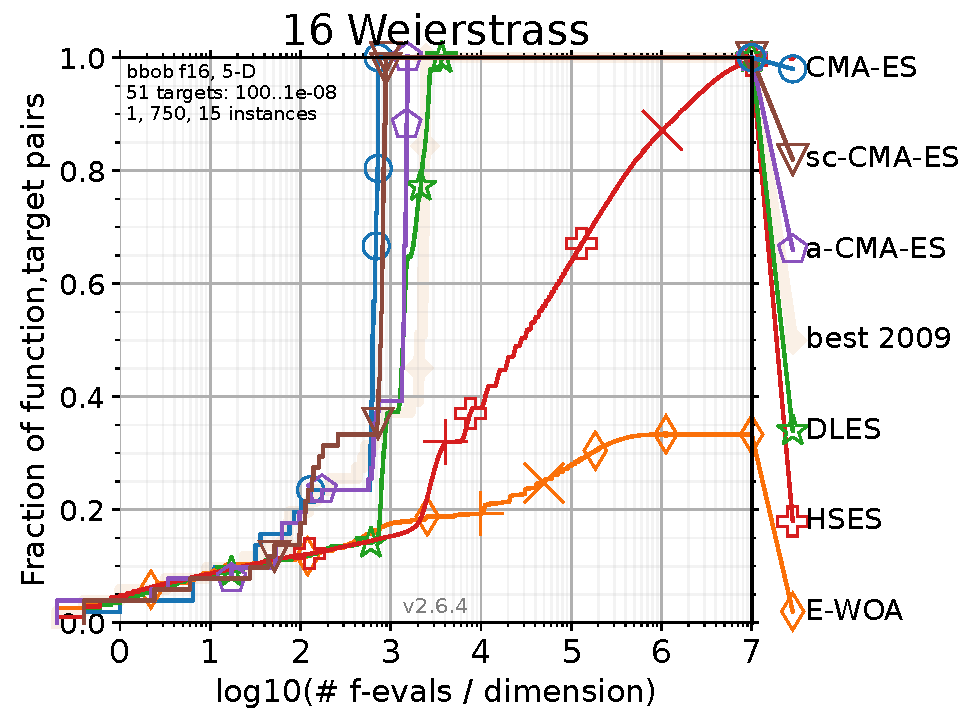
\includegraphics[width=\textwidth]{./bbob/pprldmany_f016_05D.pdf}
	\end{minipage}\hfill
	\begin{minipage}[b]{0.32\textwidth}
		\centering
		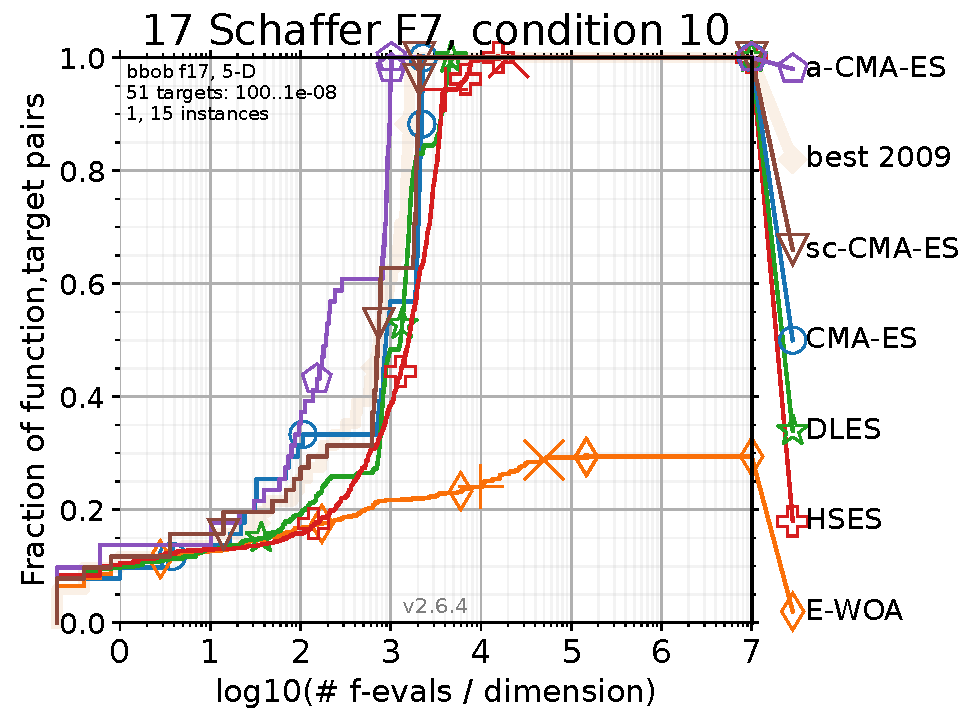
\includegraphics[width=\textwidth]{./bbob/pprldmany_f017_05D.pdf}
	\end{minipage}\hfill
	\begin{minipage}[b]{0.32\textwidth}
		\centering
		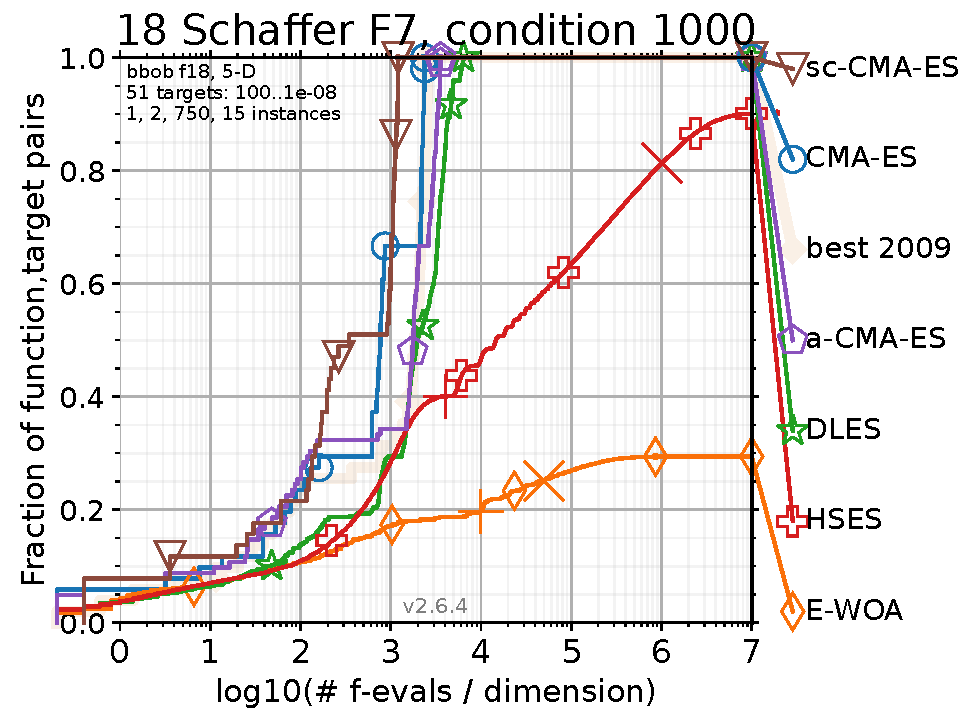
\includegraphics[width=\textwidth]{./bbob/pprldmany_f018_05D.pdf}
	\end{minipage}
	\caption{\textcolor{blue}{F16 to F18 in $D$ = 5.}}
\end{figure}

% 第七组图像
\begin{figure}[H]
	\centering
	\begin{minipage}[b]{0.32\textwidth}
		\centering
		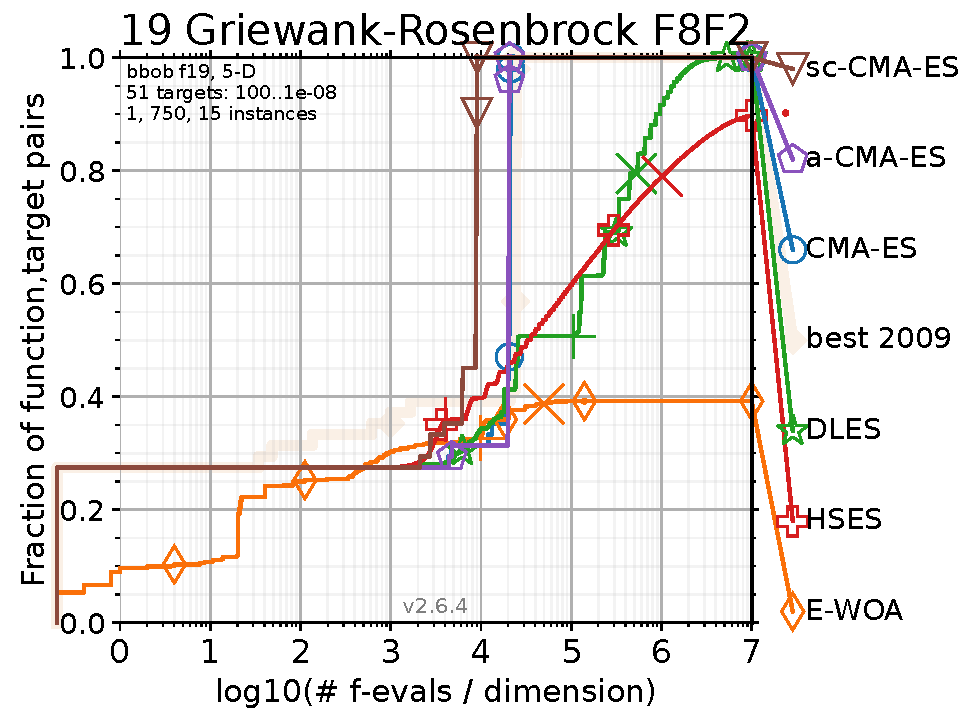
\includegraphics[width=\textwidth]{./bbob/pprldmany_f019_05D.pdf}
	\end{minipage}\hfill
	\begin{minipage}[b]{0.32\textwidth}
		\centering
		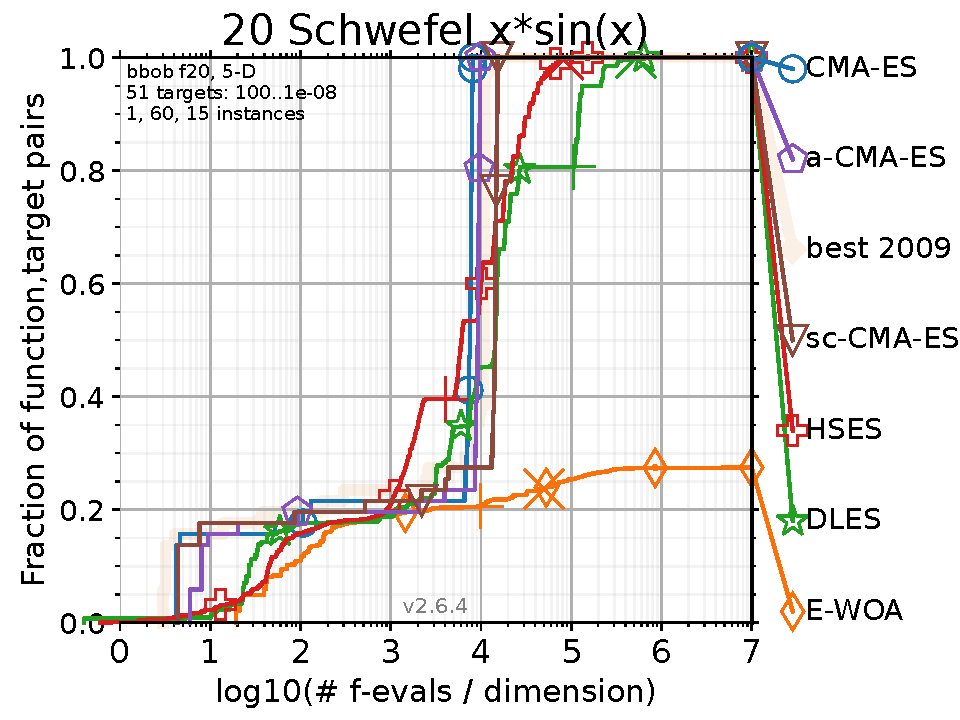
\includegraphics[width=\textwidth]{./bbob/pprldmany_f020_05D.pdf}
	\end{minipage}\hfill
	\begin{minipage}[b]{0.32\textwidth}
		\centering
		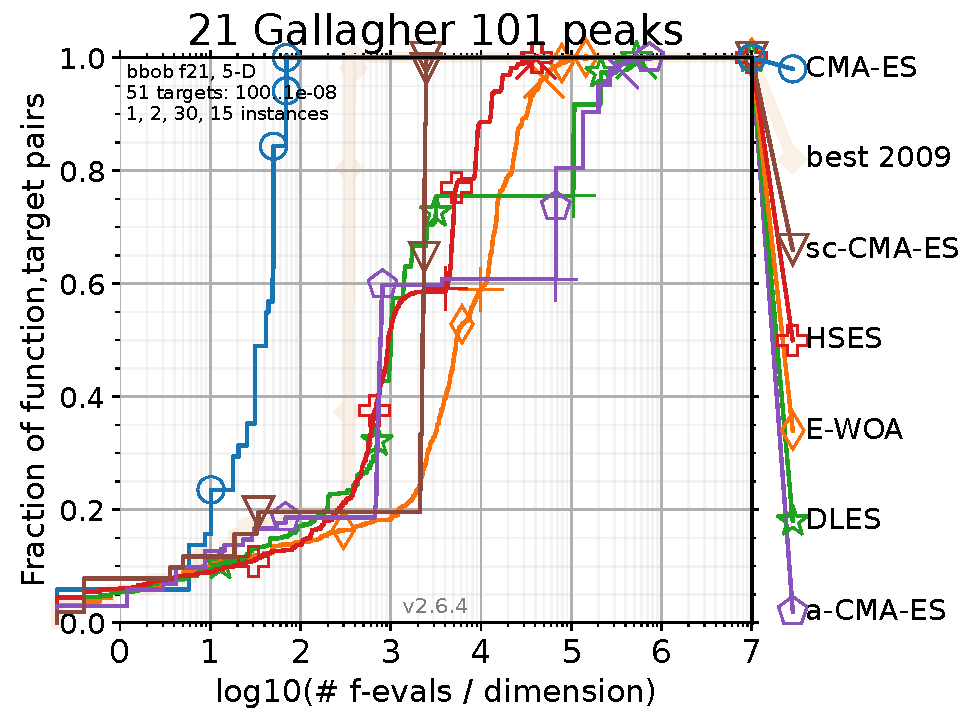
\includegraphics[width=\textwidth]{./bbob/pprldmany_f021_05D.pdf}
	\end{minipage}
	\caption{\textcolor{blue}{F19 to F21 in $D$ = 5.}}
\end{figure}

% 第八组图像
\begin{figure}[H]
	\centering
	\begin{minipage}[b]{0.32\textwidth}
		\centering
		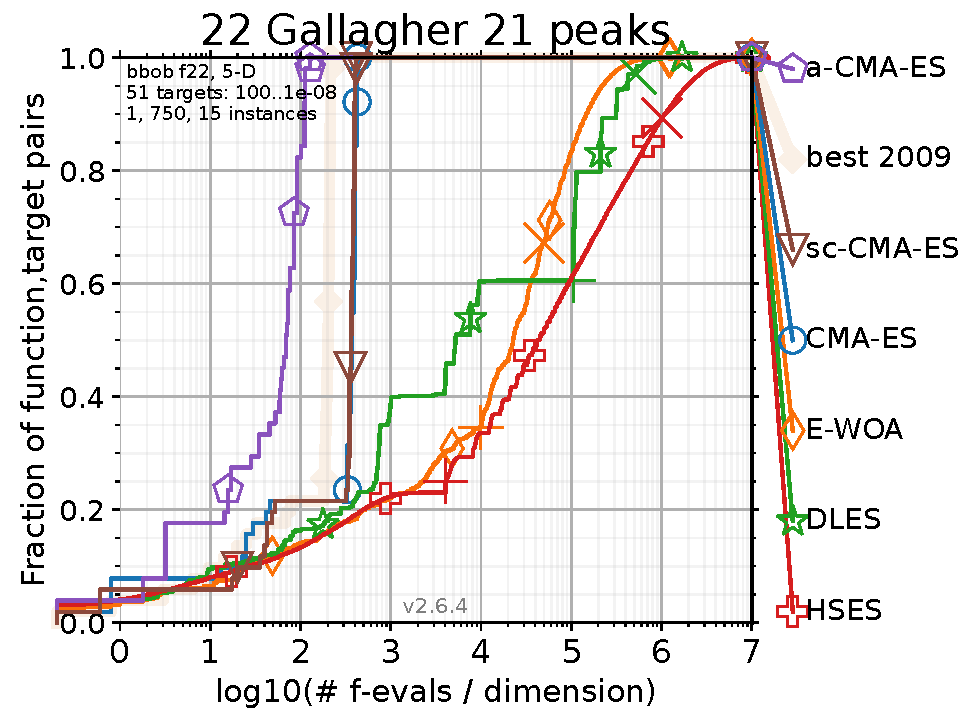
\includegraphics[width=\textwidth]{./bbob/pprldmany_f022_05D.pdf}
	\end{minipage}\hfill
	\begin{minipage}[b]{0.32\textwidth}
		\centering
		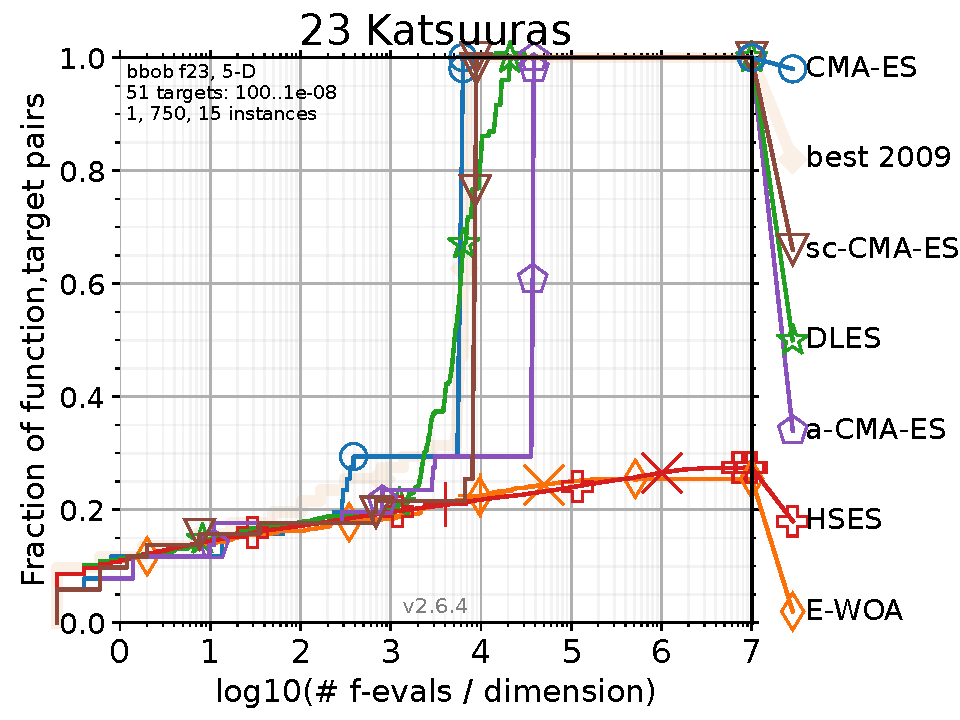
\includegraphics[width=\textwidth]{./bbob/pprldmany_f023_05D.pdf}
	\end{minipage}\hfill
	\begin{minipage}[b]{0.32\textwidth}
		\centering
		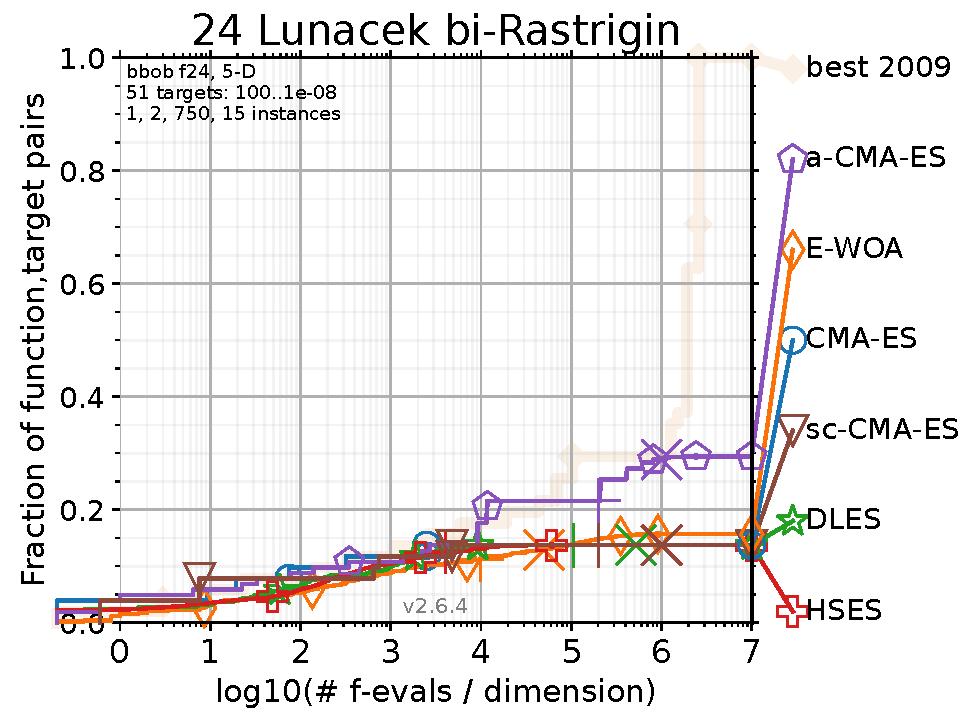
\includegraphics[width=\textwidth]{./bbob/pprldmany_f024_05D.pdf}
	\end{minipage}
	\caption{\textcolor{blue}{F22 to F24 in $D$ = 5.}}
\end{figure}

\begin{figure}[H]
	\centering
	\begin{minipage}[b]{0.32\textwidth}
		\centering
		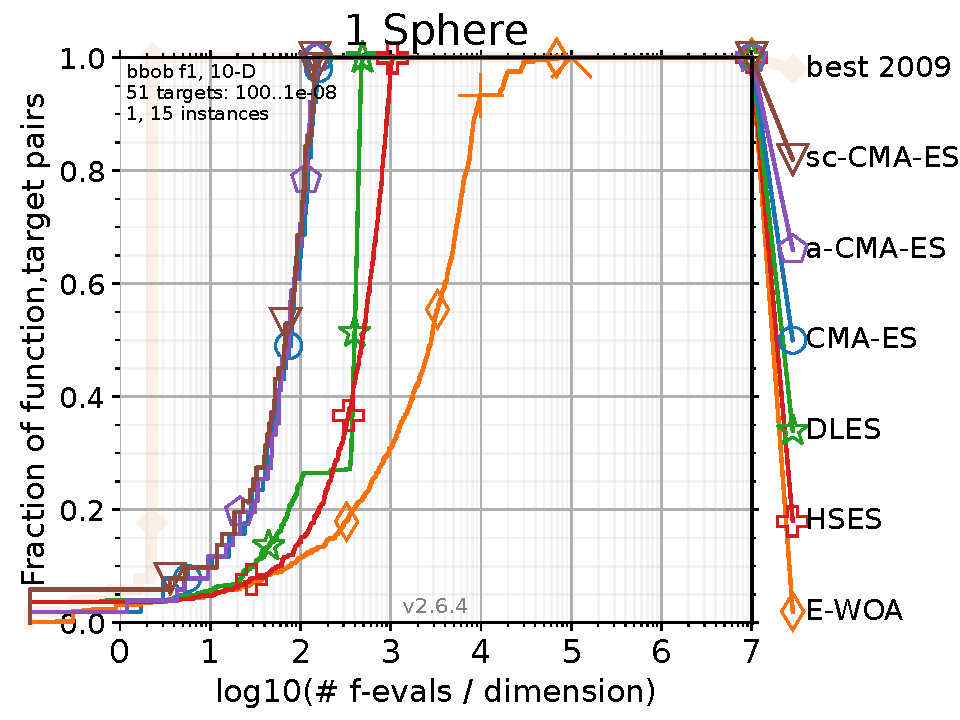
\includegraphics[width=\textwidth]{./bbob/pprldmany_f001_10D.pdf}
	\end{minipage}\hfill
	\begin{minipage}[b]{0.32\textwidth}
		\centering
		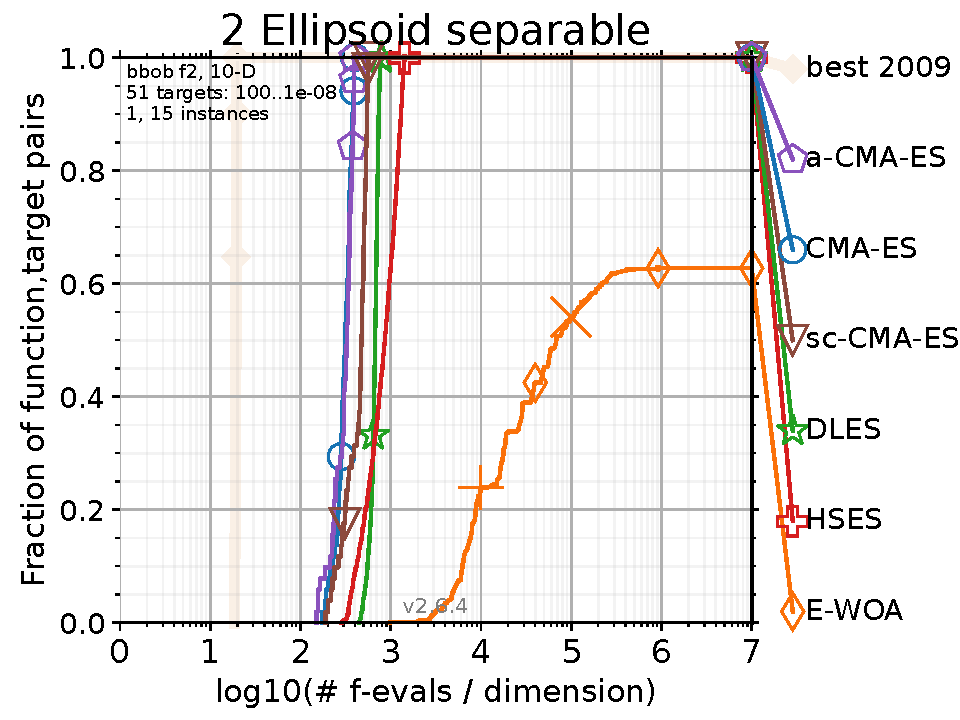
\includegraphics[width=\textwidth]{./bbob/pprldmany_f002_10D.pdf}
	\end{minipage}\hfill
	\begin{minipage}[b]{0.32\textwidth}
		\centering
		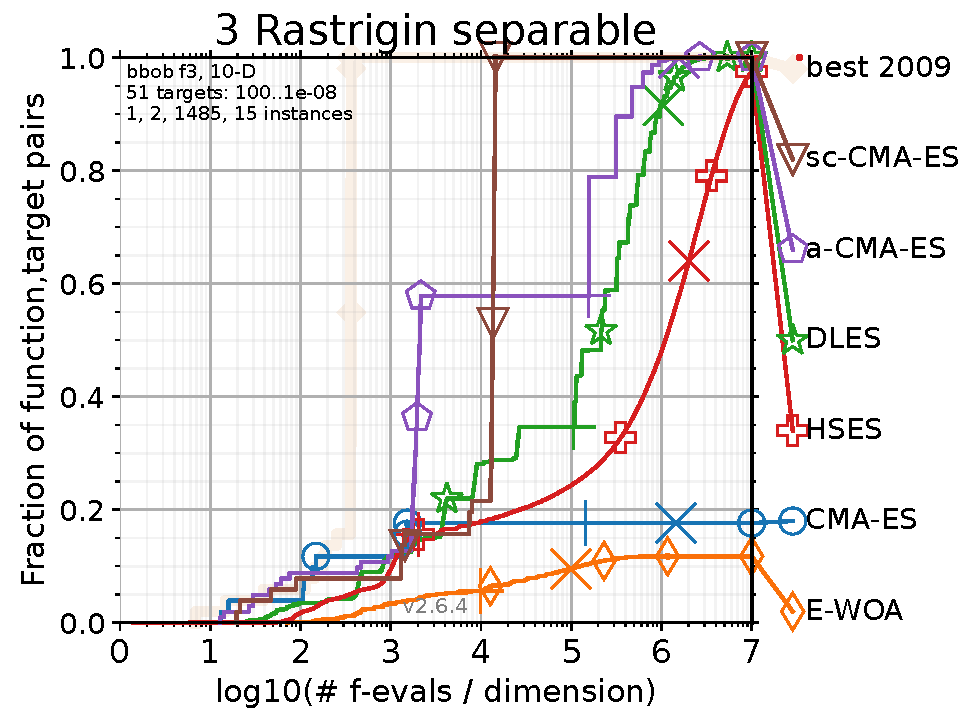
\includegraphics[width=\textwidth]{./bbob/pprldmany_f003_10D.pdf}
	\end{minipage}
	\caption{\textcolor{blue}{F1 to F3 in $D$ = 10.}}
\end{figure}

% 第二组图像
\begin{figure}[H]
	\centering
	\begin{minipage}[b]{0.32\textwidth}
		\centering
		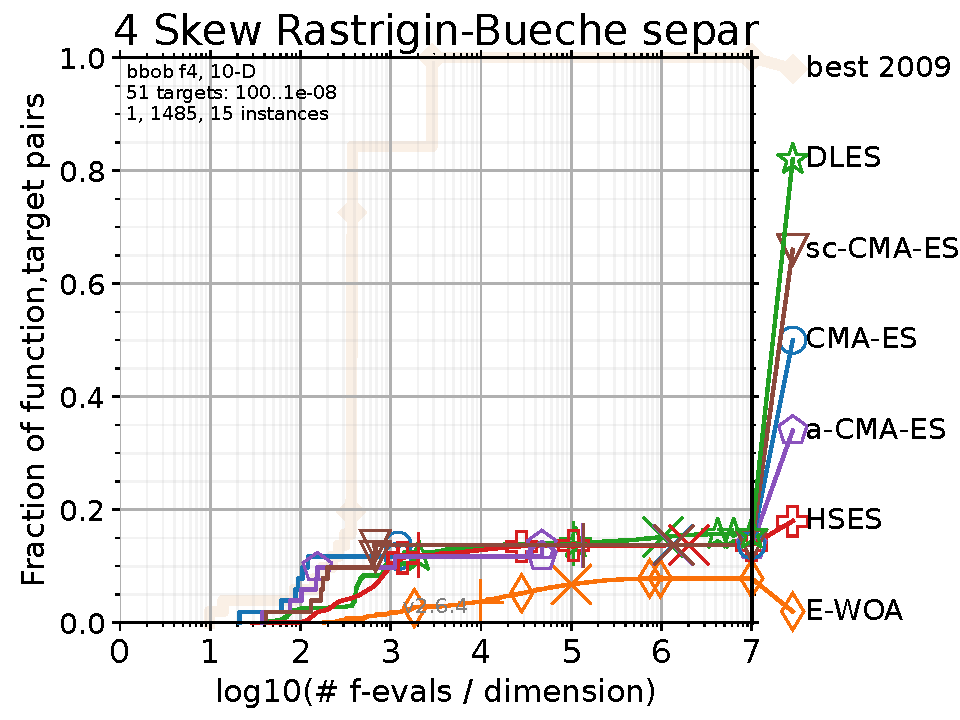
\includegraphics[width=\textwidth]{./bbob/pprldmany_f004_10D.pdf}
	\end{minipage}\hfill
	\begin{minipage}[b]{0.32\textwidth}
		\centering
		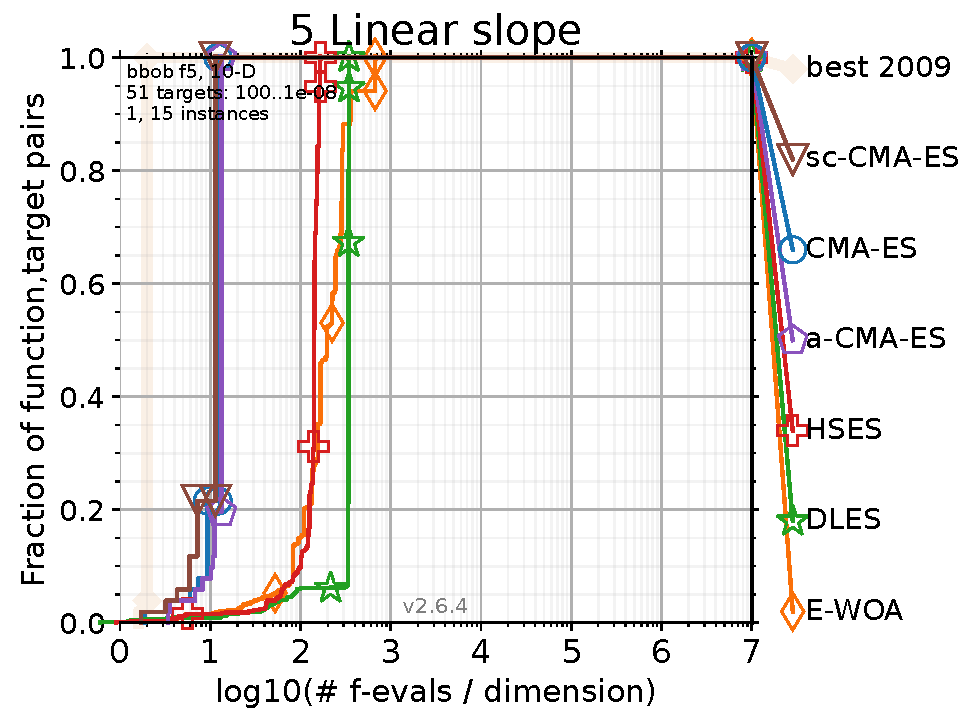
\includegraphics[width=\textwidth]{./bbob/pprldmany_f005_10D.pdf}
	\end{minipage}\hfill
	\begin{minipage}[b]{0.32\textwidth}
		\centering
		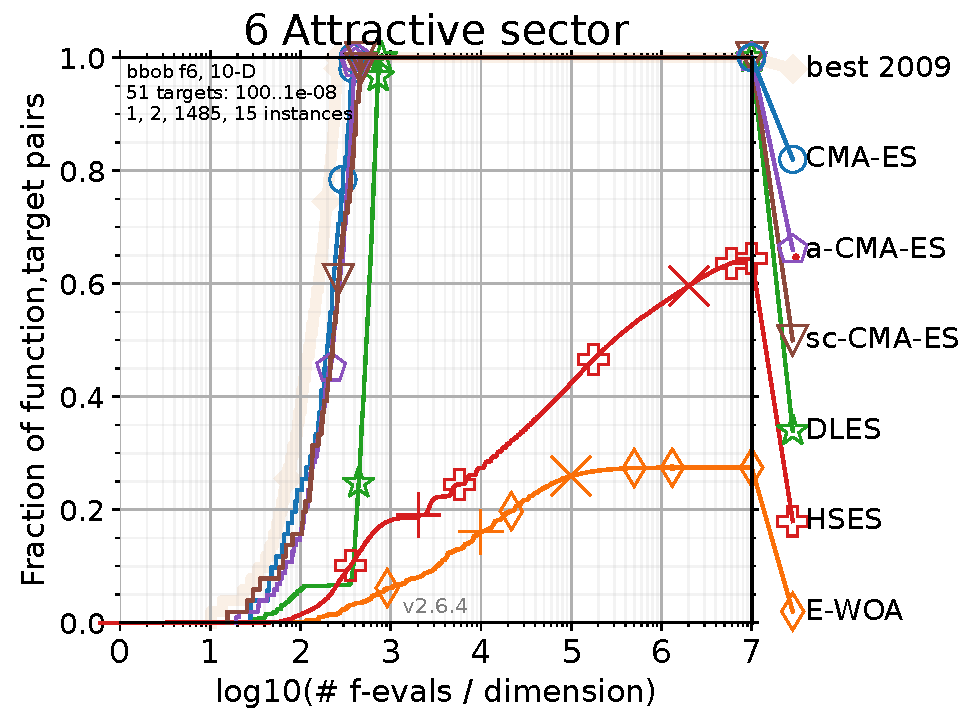
\includegraphics[width=\textwidth]{./bbob/pprldmany_f006_10D.pdf}
	\end{minipage}
	\caption{\textcolor{blue}{F4 to F6 in $D$ = 10.}}
\end{figure}

% 第三组图像
\begin{figure}[H]
	\centering
	\begin{minipage}[b]{0.32\textwidth}
		\centering
		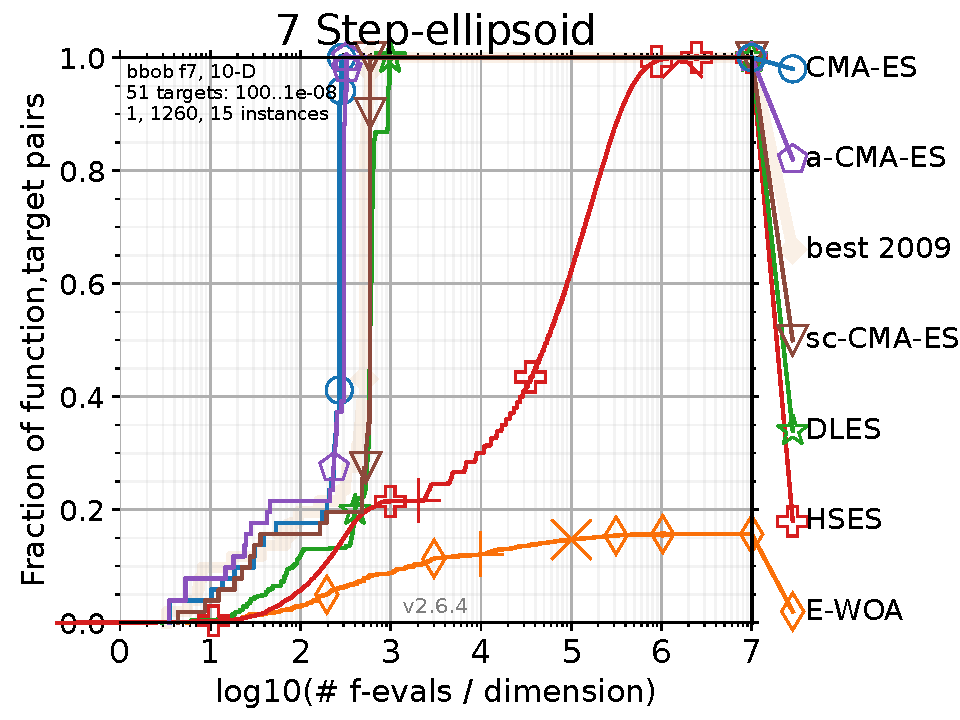
\includegraphics[width=\textwidth]{./bbob/pprldmany_f007_10D.pdf}
	\end{minipage}\hfill
	\begin{minipage}[b]{0.32\textwidth}
		\centering
		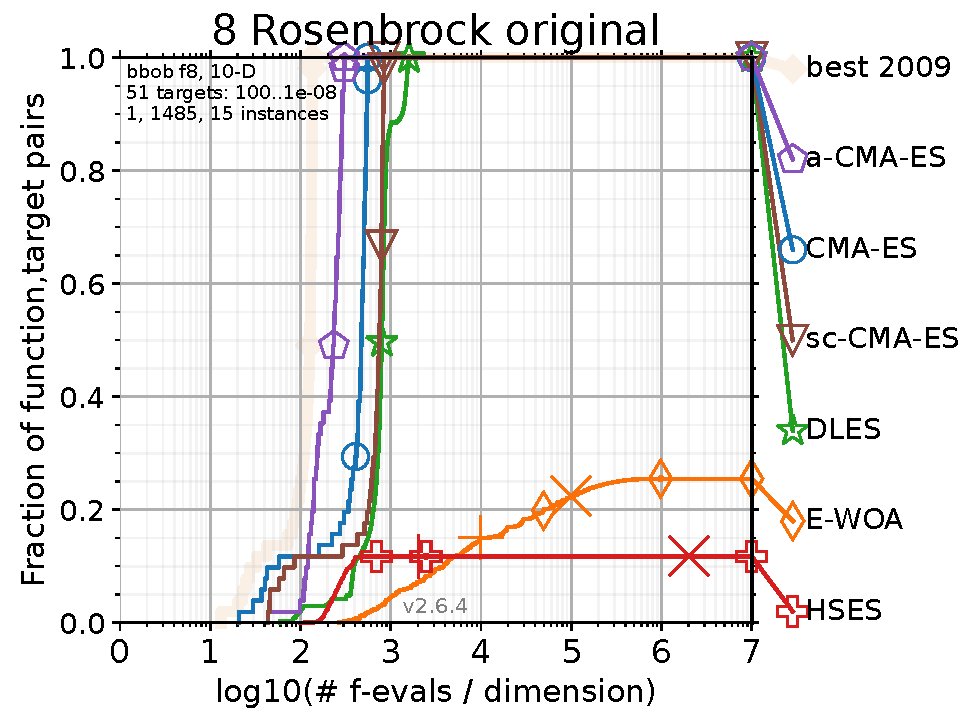
\includegraphics[width=\textwidth]{./bbob/pprldmany_f008_10D.pdf}
	\end{minipage}\hfill
	\begin{minipage}[b]{0.32\textwidth}
		\centering
		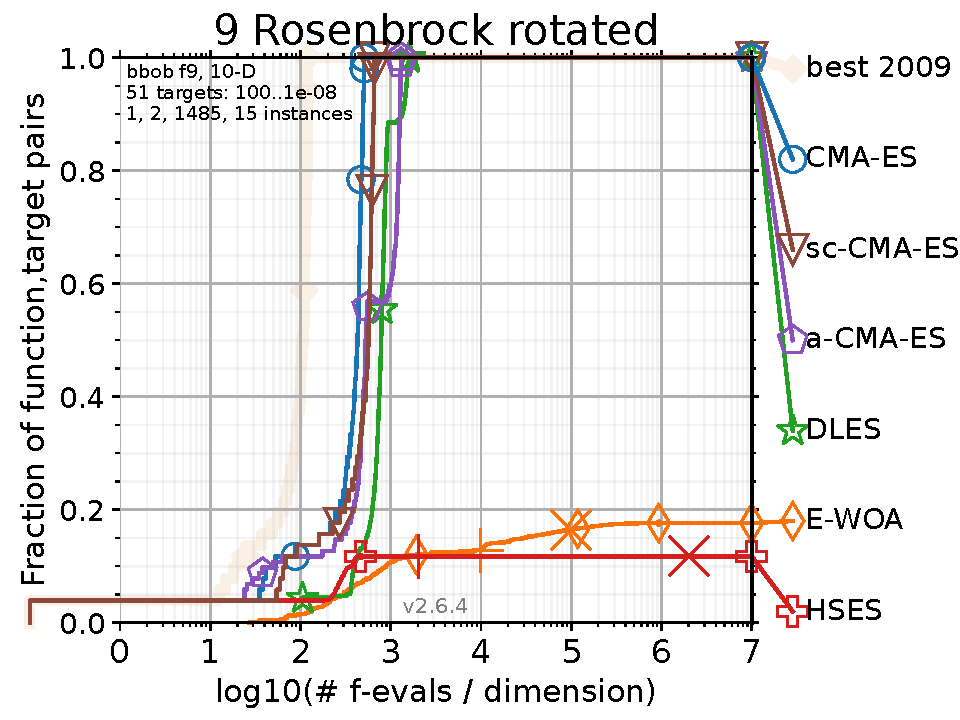
\includegraphics[width=\textwidth]{./bbob/pprldmany_f009_10D.pdf}
	\end{minipage}
	\caption{\textcolor{blue}{F7 to F9 in $D$ = 10.}}
\end{figure}

% 第四组图像
\begin{figure}[H]
	\centering
	\begin{minipage}[b]{0.32\textwidth}
		\centering
		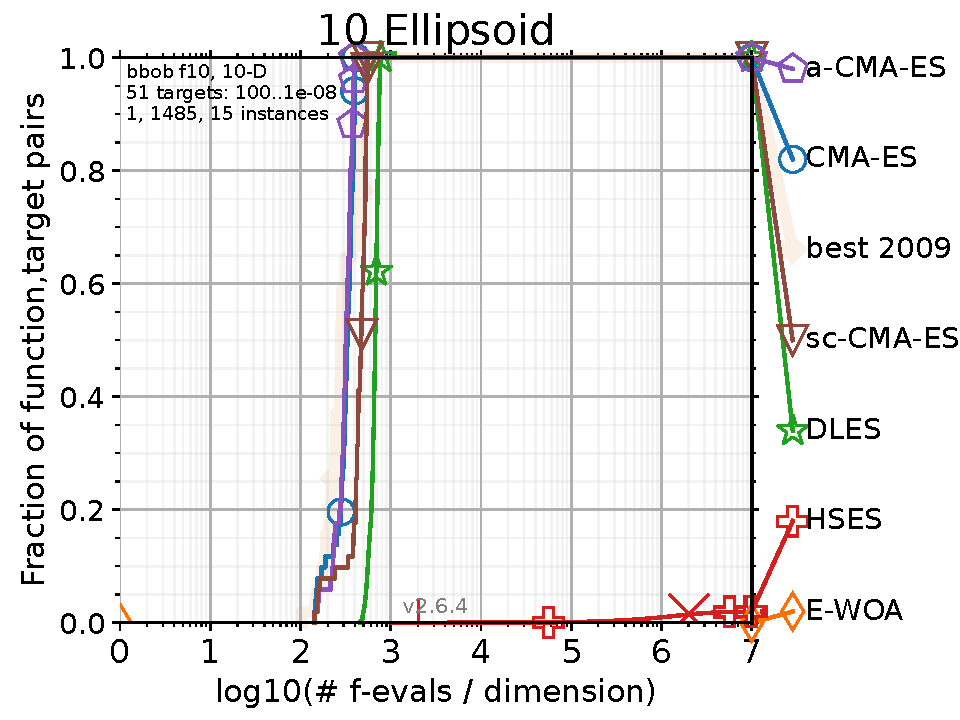
\includegraphics[width=\textwidth]{./bbob/pprldmany_f010_10D.pdf}
	\end{minipage}\hfill
	\begin{minipage}[b]{0.32\textwidth}
		\centering
		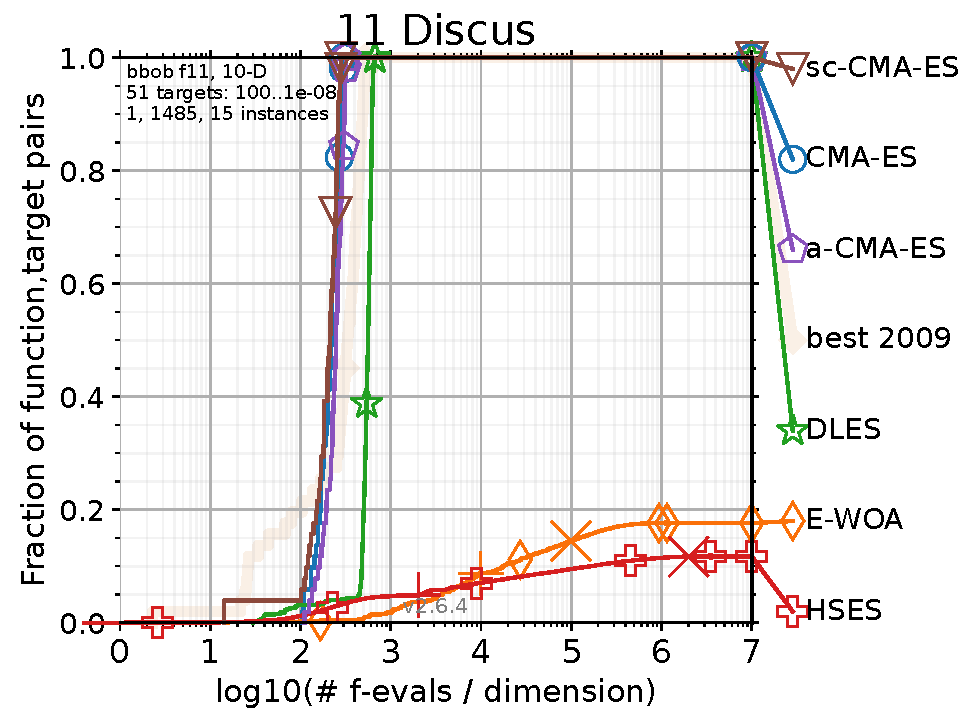
\includegraphics[width=\textwidth]{./bbob/pprldmany_f011_10D.pdf}
	\end{minipage}\hfill
	\begin{minipage}[b]{0.32\textwidth}
		\centering
		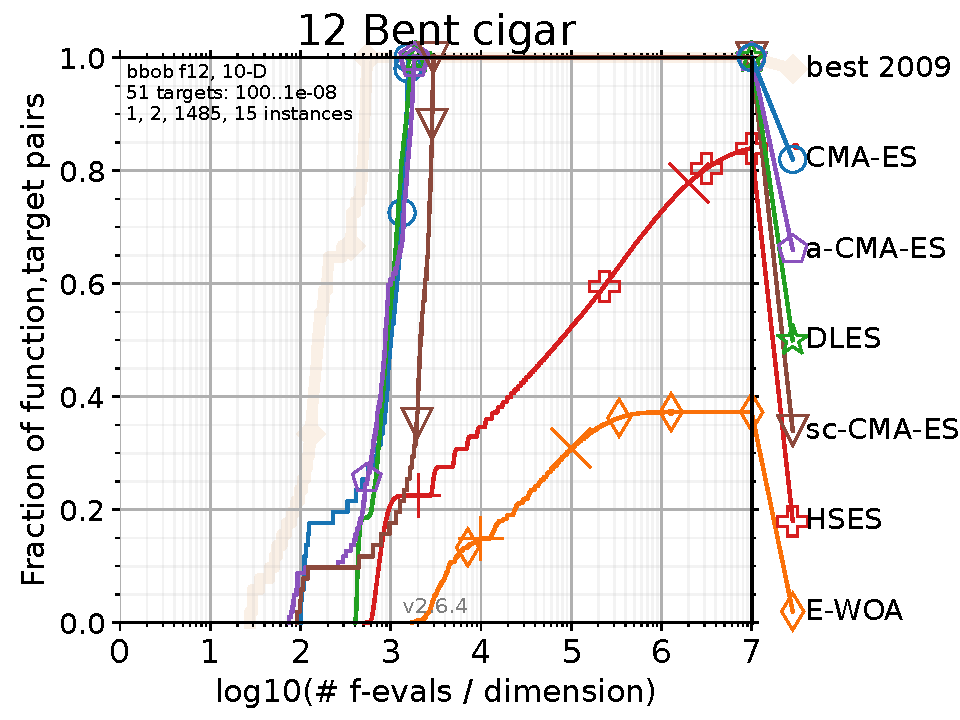
\includegraphics[width=\textwidth]{./bbob/pprldmany_f012_10D.pdf}
	\end{minipage}
	\caption{\textcolor{blue}{F10 to F12 in $D$ = 10.}}
\end{figure}

% 第五组图像
\begin{figure}[H]
	\centering
	\begin{minipage}[b]{0.32\textwidth}
		\centering
		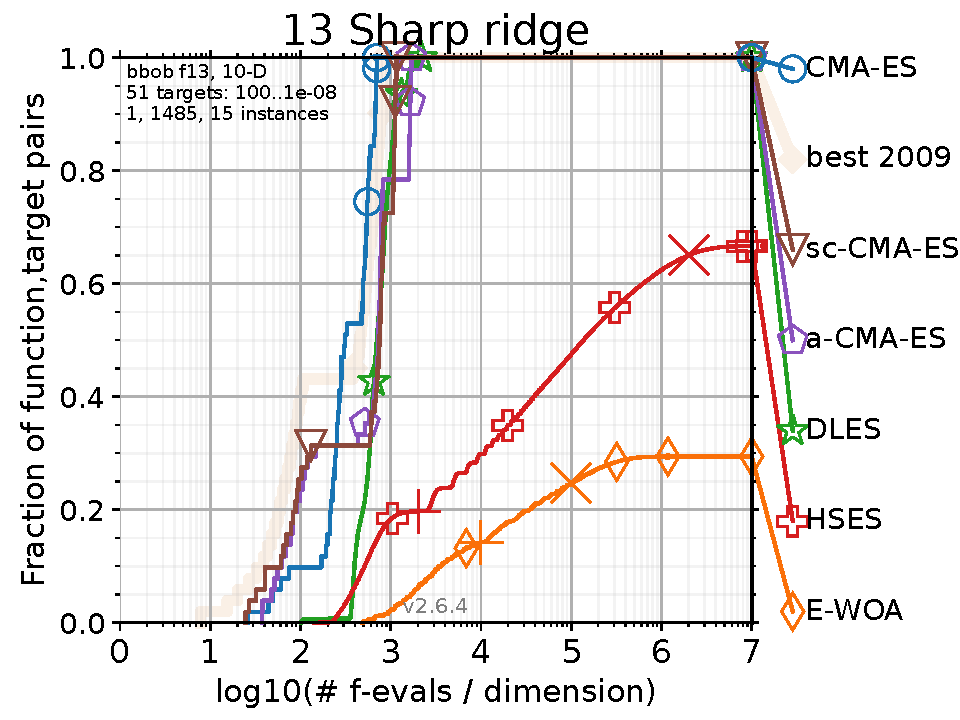
\includegraphics[width=\textwidth]{./bbob/pprldmany_f013_10D.pdf}
	\end{minipage}\hfill
	\begin{minipage}[b]{0.32\textwidth}
		\centering
		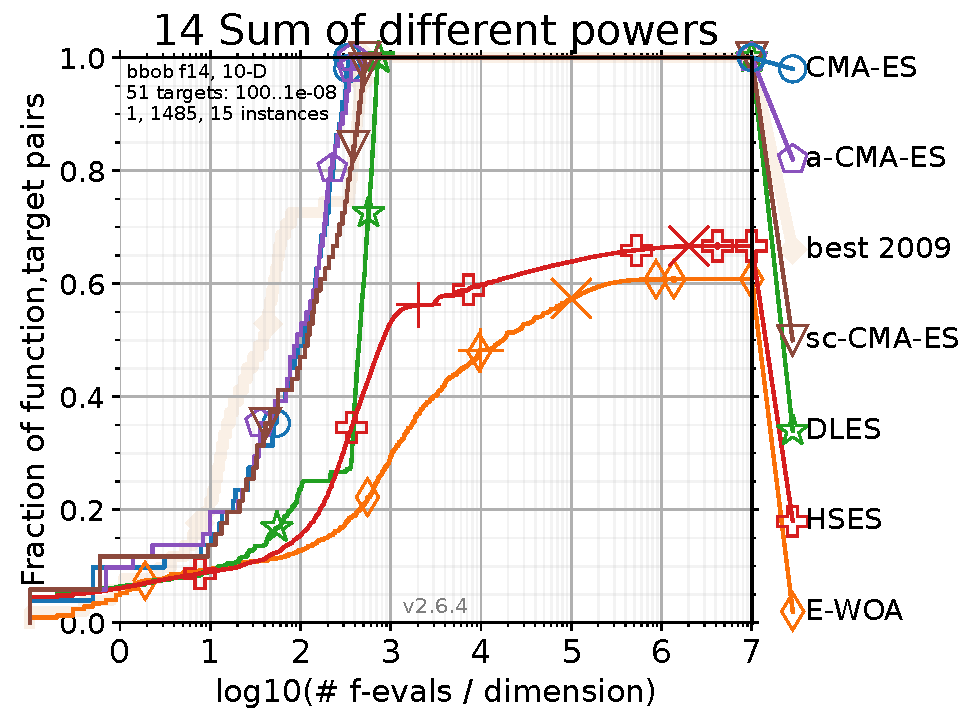
\includegraphics[width=\textwidth]{./bbob/pprldmany_f014_10D.pdf}
	\end{minipage}\hfill
	\begin{minipage}[b]{0.32\textwidth}
		\centering
		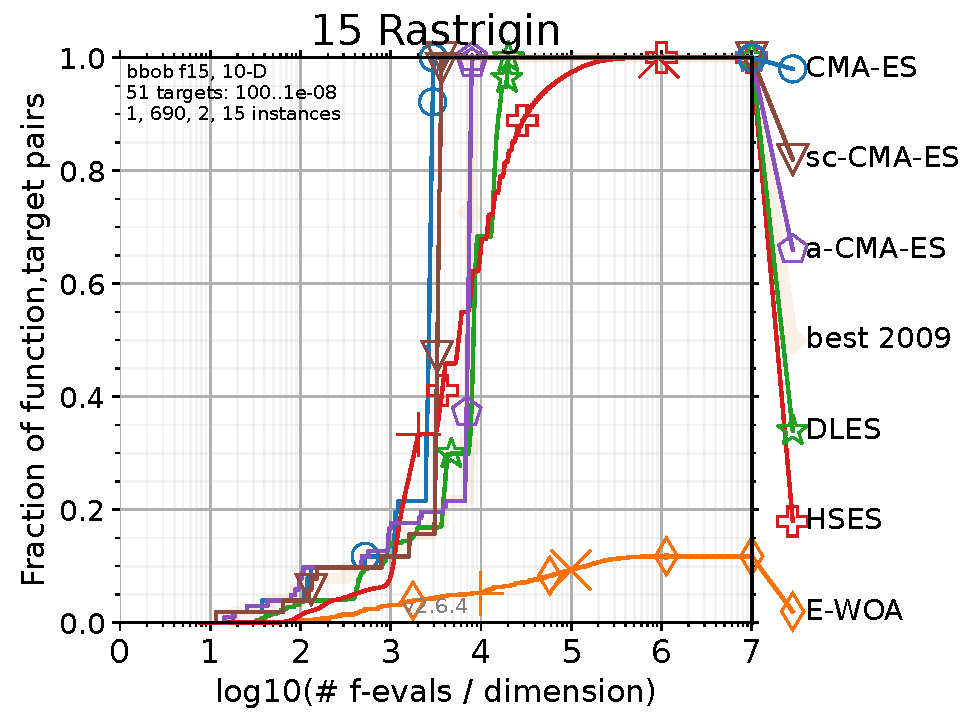
\includegraphics[width=\textwidth]{./bbob/pprldmany_f015_10D.pdf}
	\end{minipage}
	\caption{\textcolor{blue}{F13 to F15 in $D$ = 10.}}
\end{figure}

% 第六组图像
\begin{figure}[H]
	\centering
	\begin{minipage}[b]{0.32\textwidth}
		\centering
		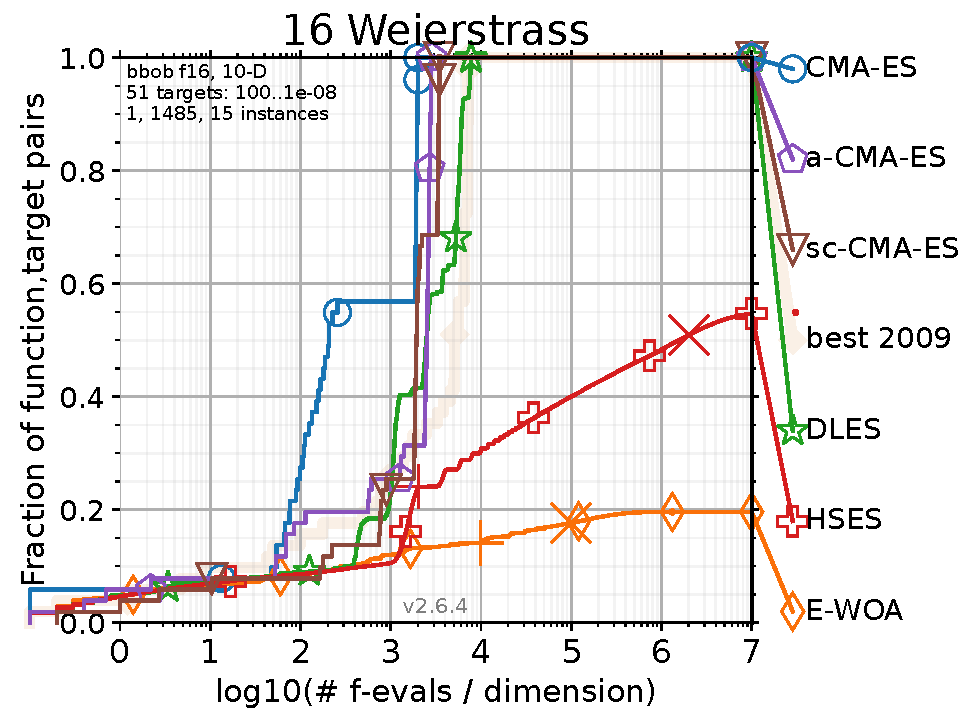
\includegraphics[width=\textwidth]{./bbob/pprldmany_f016_10D.pdf}
	\end{minipage}\hfill
	\begin{minipage}[b]{0.32\textwidth}
		\centering
		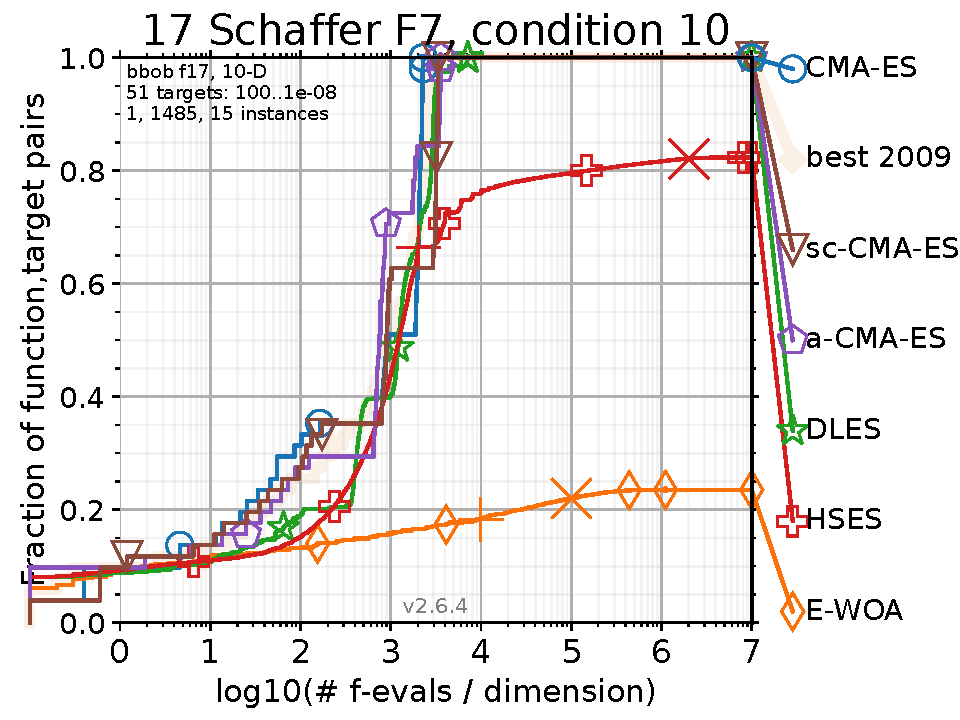
\includegraphics[width=\textwidth]{./bbob/pprldmany_f017_10D.pdf}
	\end{minipage}\hfill
	\begin{minipage}[b]{0.32\textwidth}
		\centering
		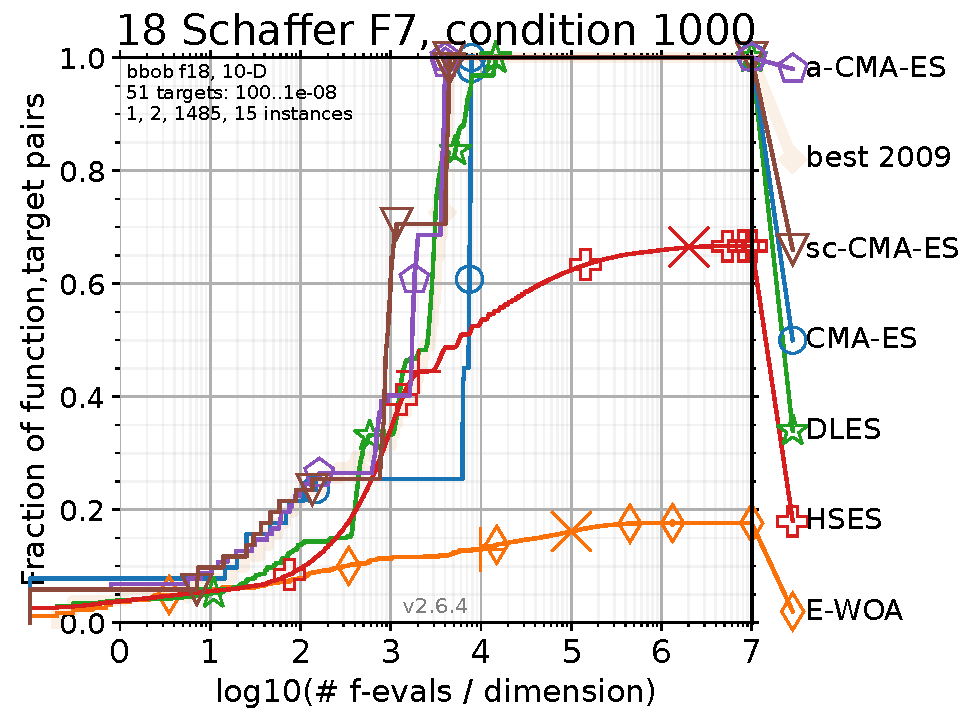
\includegraphics[width=\textwidth]{./bbob/pprldmany_f018_10D.pdf}
	\end{minipage}
	\caption{\textcolor{blue}{F16 to F18 in $D$ = 10.}}
\end{figure}

% 第七组图像
\begin{figure}[H]
	\centering
	\begin{minipage}[b]{0.32\textwidth}
		\centering
		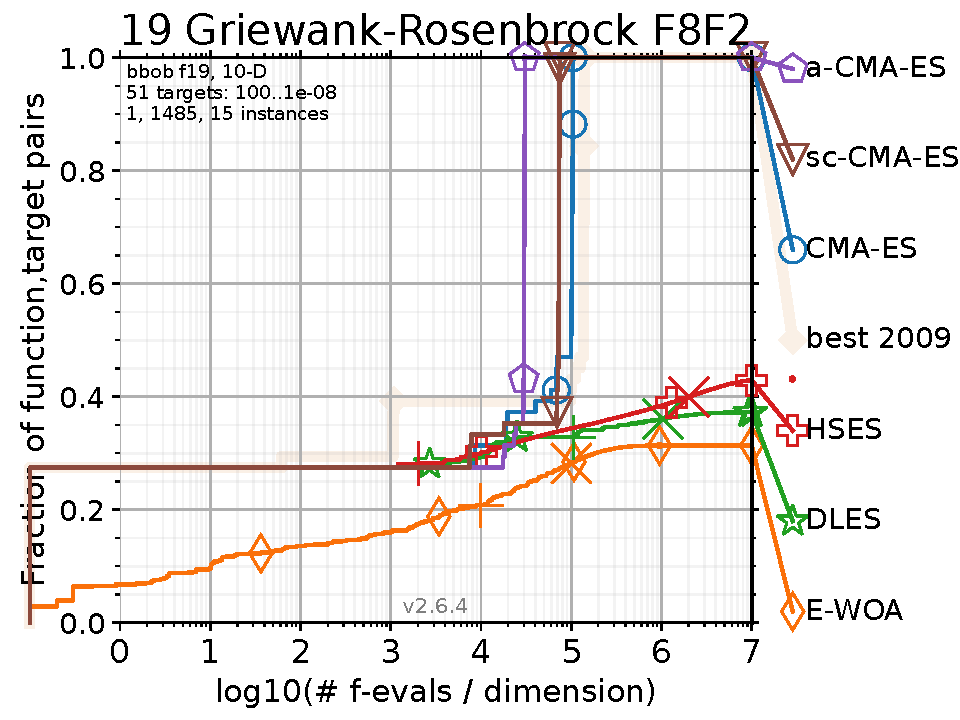
\includegraphics[width=\textwidth]{./bbob/pprldmany_f019_10D.pdf}
	\end{minipage}\hfill
	\begin{minipage}[b]{0.32\textwidth}
		\centering
		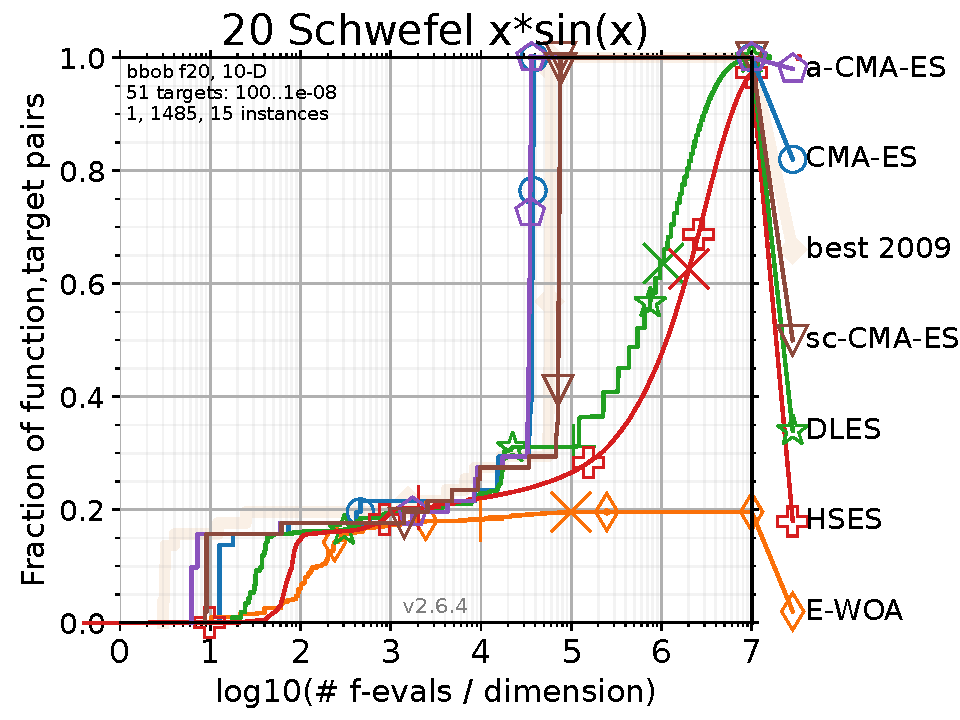
\includegraphics[width=\textwidth]{./bbob/pprldmany_f020_10D.pdf}
	\end{minipage}\hfill
	\begin{minipage}[b]{0.32\textwidth}
		\centering
		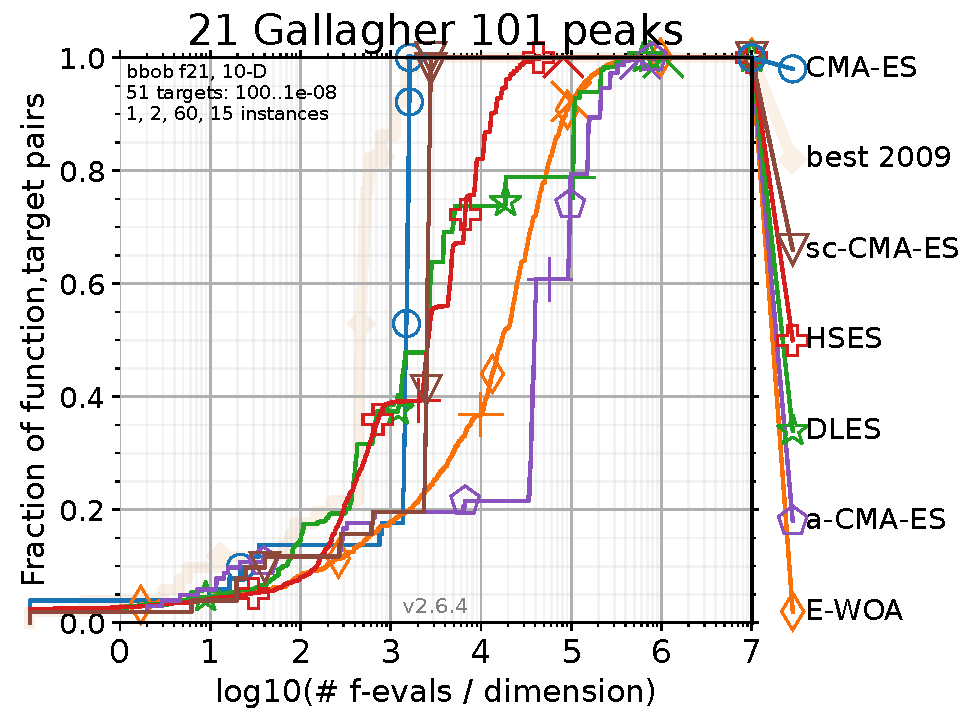
\includegraphics[width=\textwidth]{./bbob/pprldmany_f021_10D.pdf}
	\end{minipage}
	\caption{\textcolor{blue}{F19 to F21 in $D$ = 10.}}
\end{figure}

% 第八组图像
\begin{figure}[H]
	\centering
	\begin{minipage}[b]{0.32\textwidth}
		\centering
		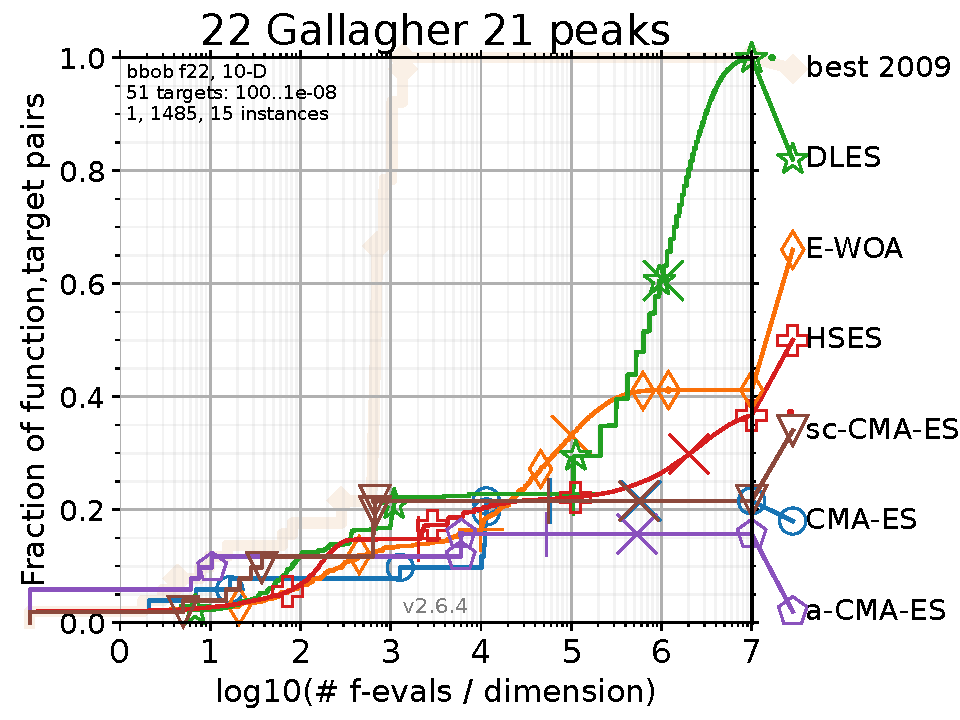
\includegraphics[width=\textwidth]{./bbob/pprldmany_f022_10D.pdf}
	\end{minipage}\hfill
	\begin{minipage}[b]{0.32\textwidth}
		\centering
		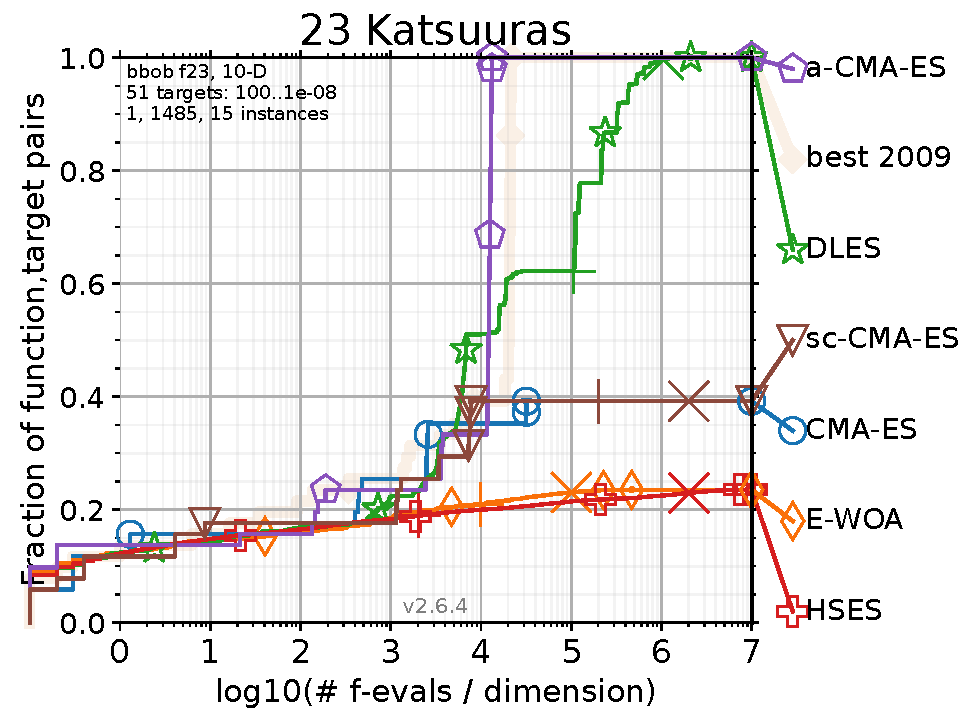
\includegraphics[width=\textwidth]{./bbob/pprldmany_f023_10D.pdf}
	\end{minipage}\hfill
	\begin{minipage}[b]{0.32\textwidth}
		\centering
		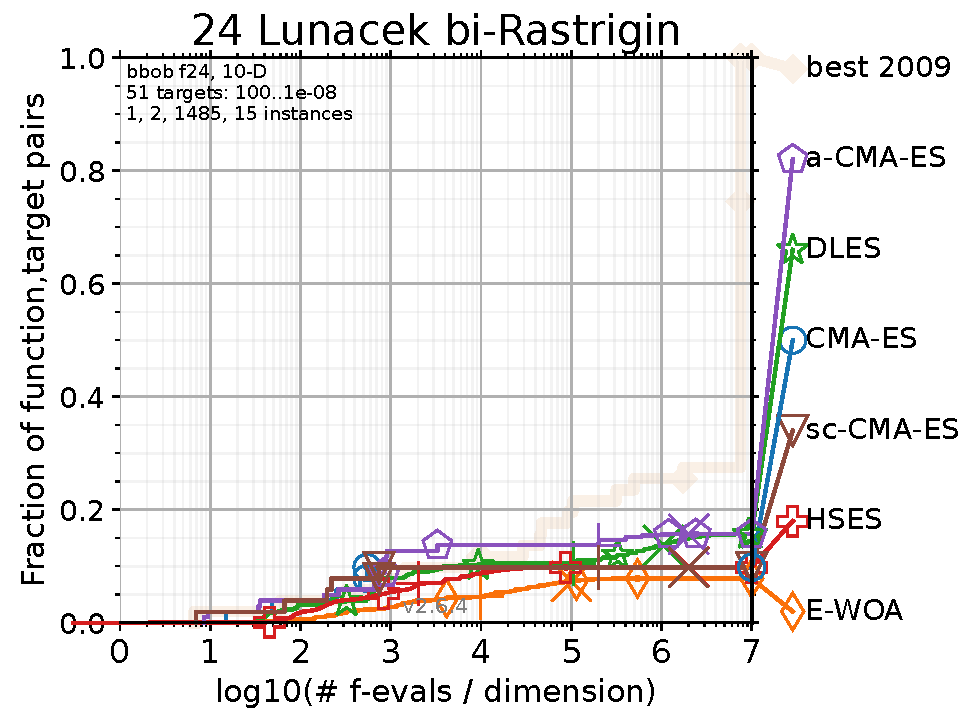
\includegraphics[width=\textwidth]{./bbob/pprldmany_f024_10D.pdf}
	\end{minipage}
	\caption{\textcolor{blue}{F22 to F24 in $D$ = 10.}}
\end{figure}

% 第一个组图像
\begin{figure}[H]
	\centering
	\begin{minipage}[b]{0.32\textwidth}
		\centering
		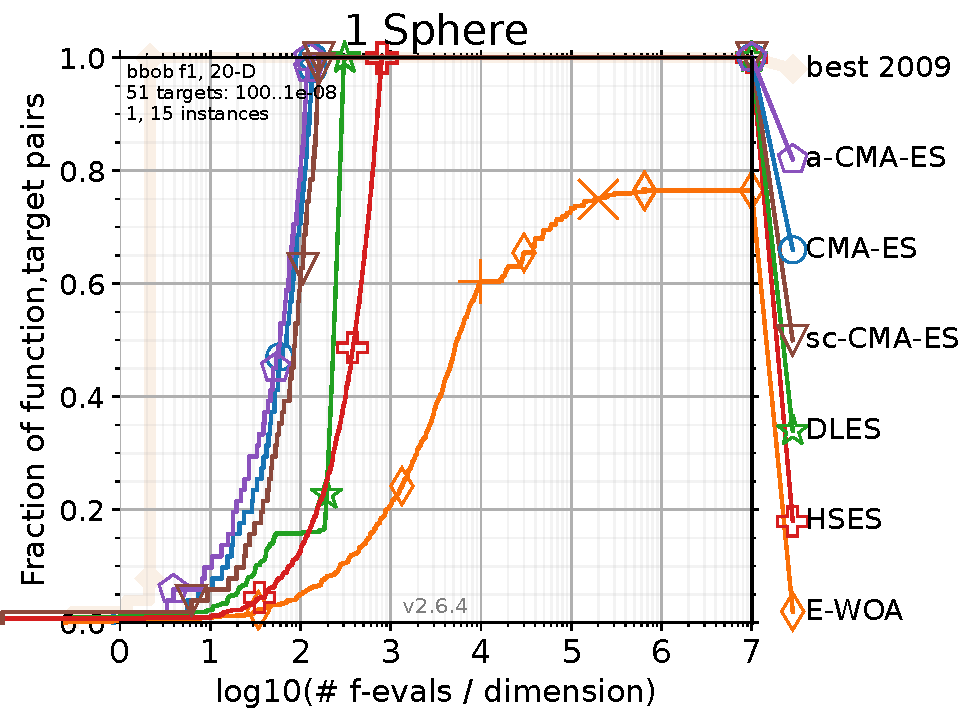
\includegraphics[width=\textwidth]{./bbob/pprldmany_f001_20D.pdf}
	\end{minipage}\hfill
	\begin{minipage}[b]{0.32\textwidth}
		\centering
		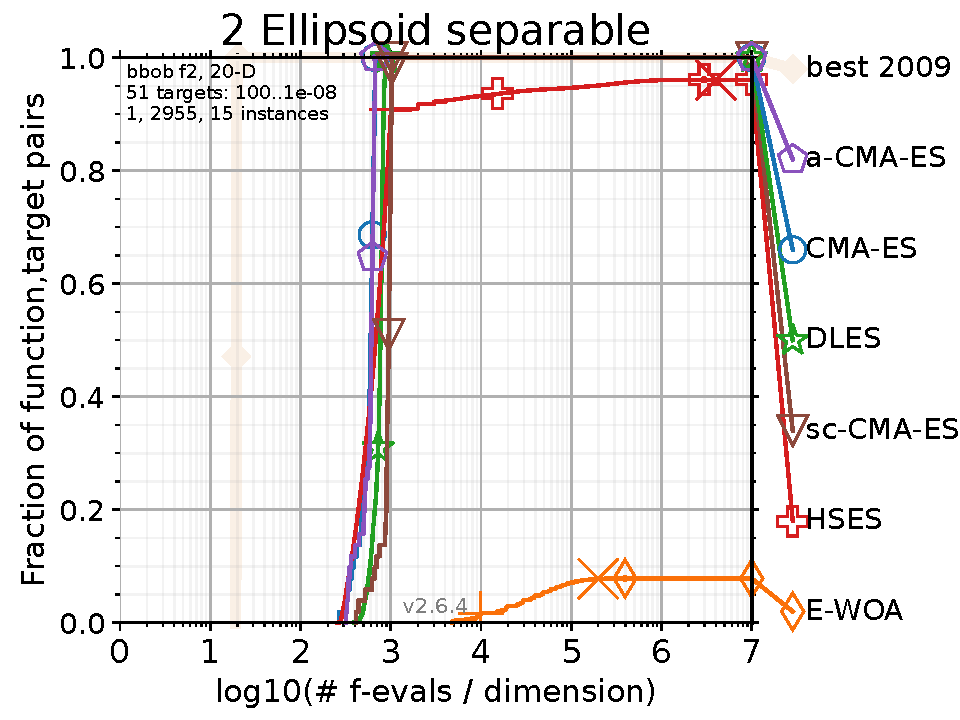
\includegraphics[width=\textwidth]{./bbob/pprldmany_f002_20D.pdf}
	\end{minipage}\hfill
	\begin{minipage}[b]{0.32\textwidth}
		\centering
		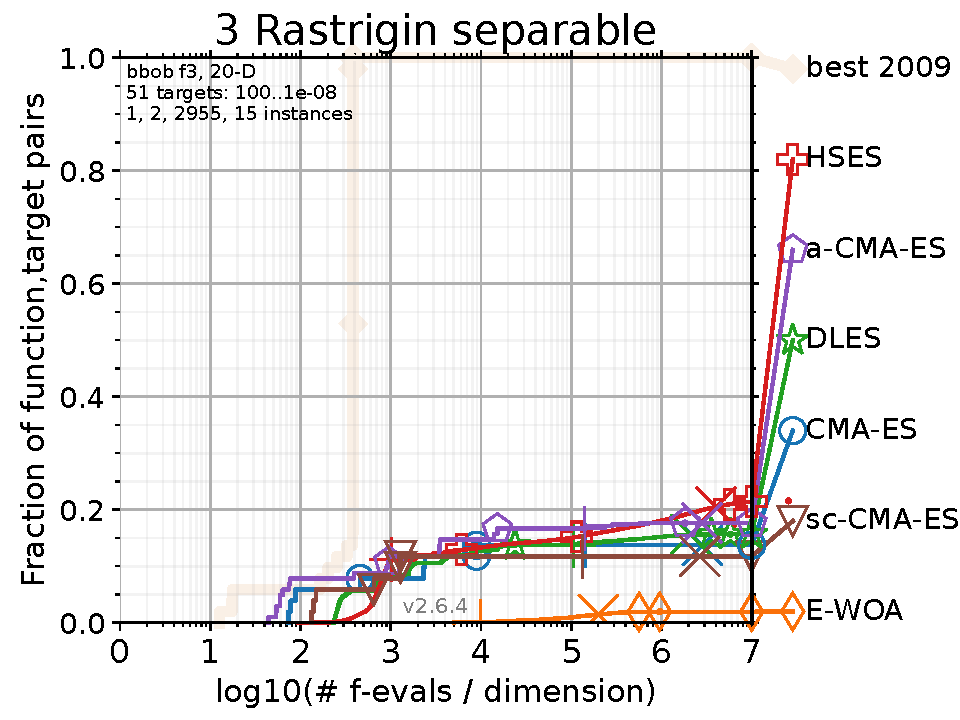
\includegraphics[width=\textwidth]{./bbob/pprldmany_f003_20D.pdf}
	\end{minipage}
	\caption{\textcolor{blue}{F1 to F3 in $D$ = 20.}}
\end{figure}

% 第二组图像
\begin{figure}[H]
	\centering
	\begin{minipage}[b]{0.32\textwidth}
		\centering
		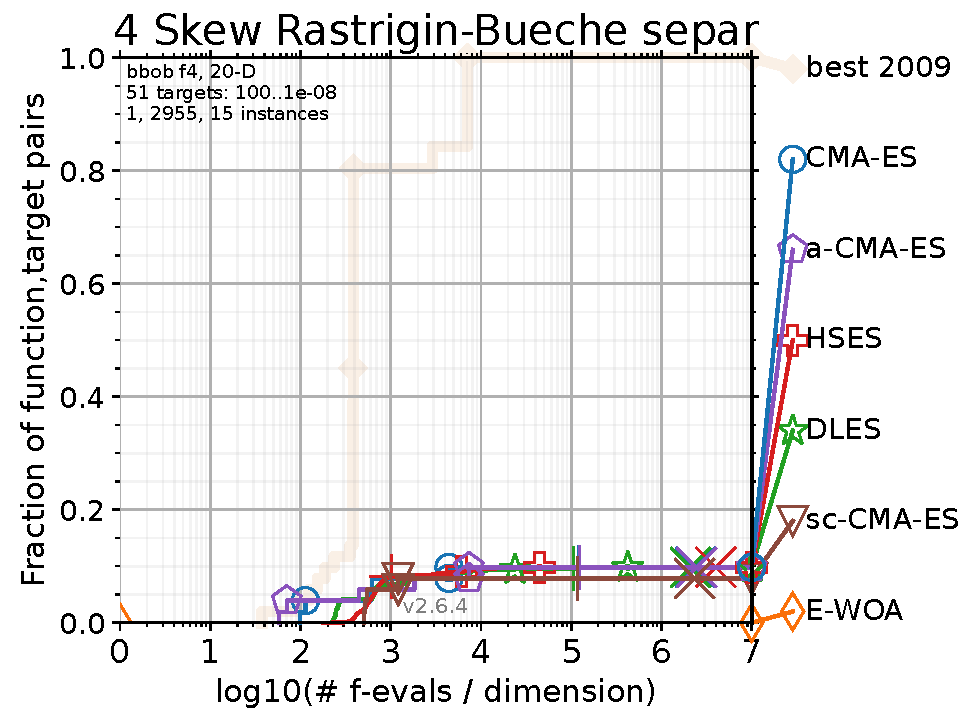
\includegraphics[width=\textwidth]{./bbob/pprldmany_f004_20D.pdf}
	\end{minipage}\hfill
	\begin{minipage}[b]{0.32\textwidth}
		\centering
		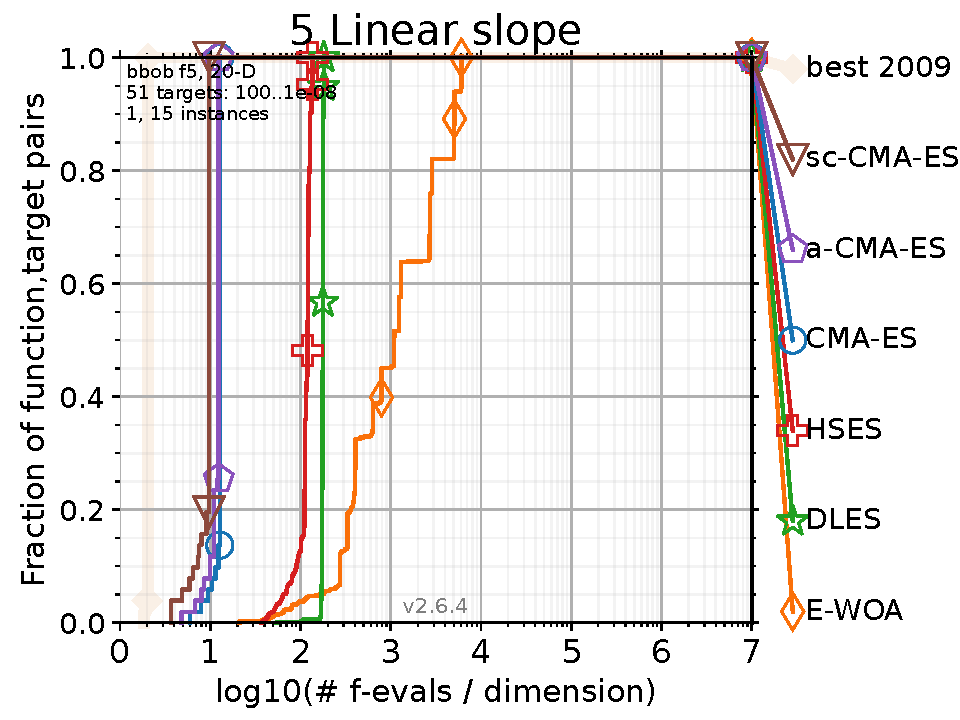
\includegraphics[width=\textwidth]{./bbob/pprldmany_f005_20D.pdf}
	\end{minipage}\hfill
	\begin{minipage}[b]{0.32\textwidth}
		\centering
		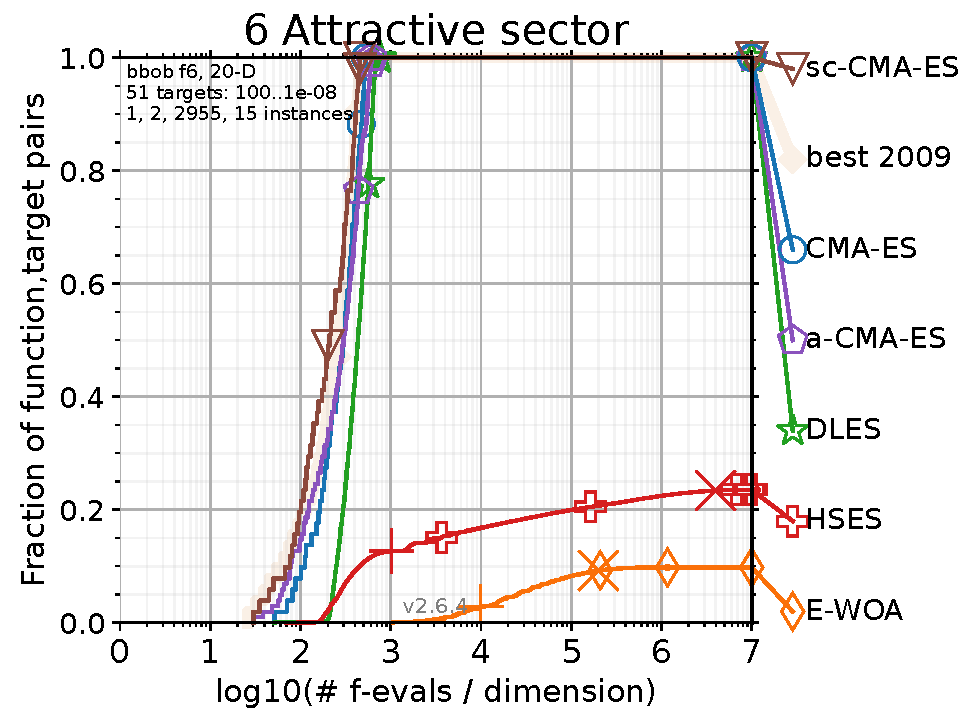
\includegraphics[width=\textwidth]{./bbob/pprldmany_f006_20D.pdf}
	\end{minipage}
	\caption{\textcolor{blue}{F4 to F6 in $D$ = 20.}}
\end{figure}

% 第三组图像
\begin{figure}[H]
	\centering
	\begin{minipage}[b]{0.32\textwidth}
		\centering
		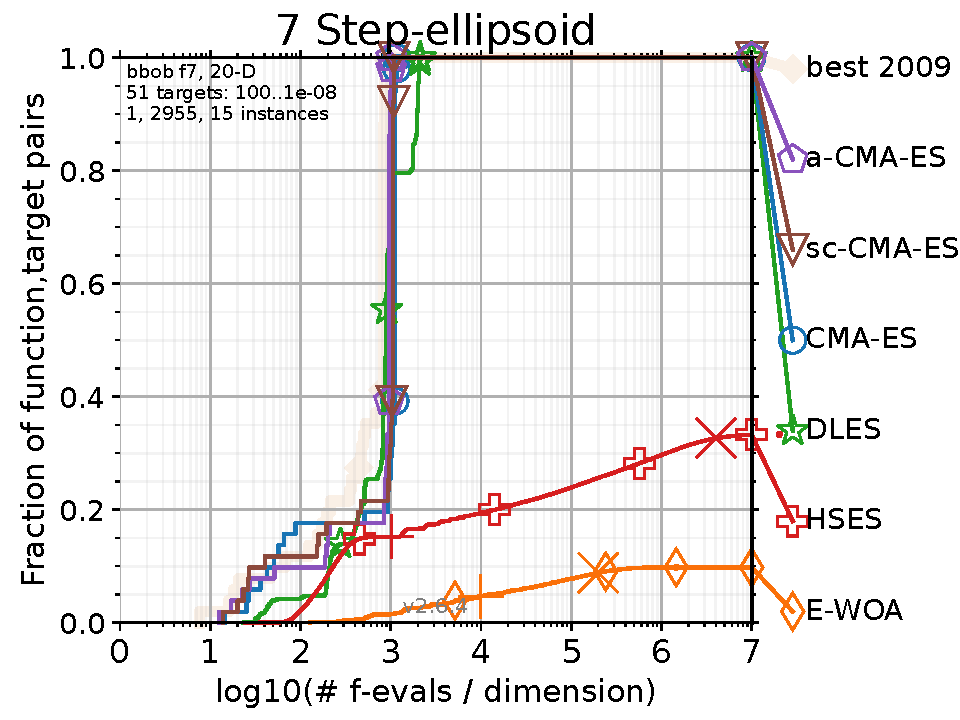
\includegraphics[width=\textwidth]{./bbob/pprldmany_f007_20D.pdf}
	\end{minipage}\hfill
	\begin{minipage}[b]{0.32\textwidth}
		\centering
		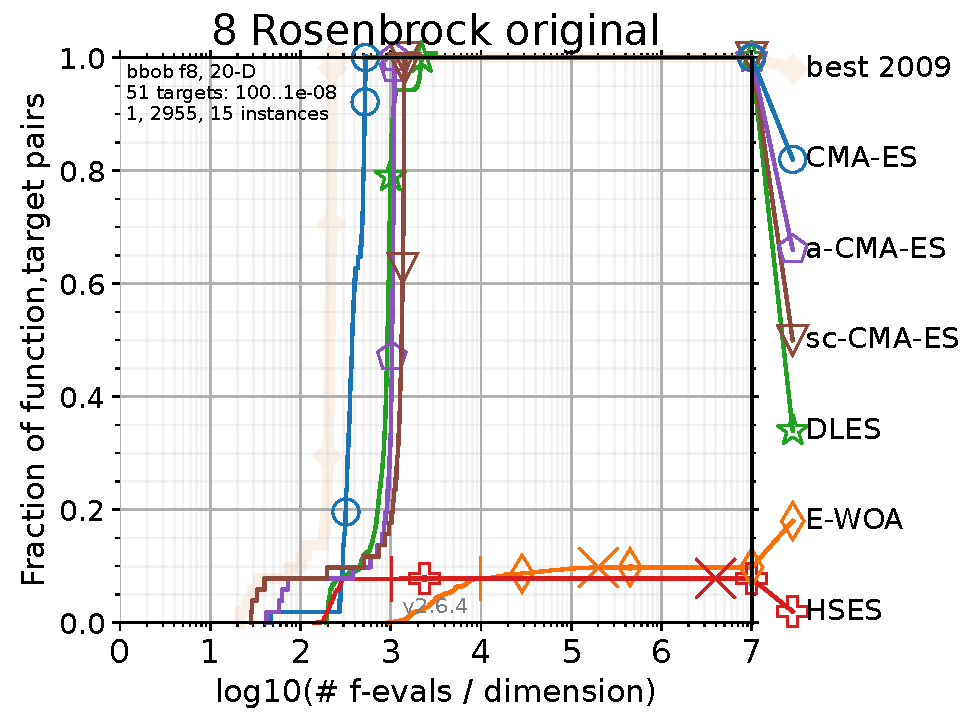
\includegraphics[width=\textwidth]{./bbob/pprldmany_f008_20D.pdf}
	\end{minipage}\hfill
	\begin{minipage}[b]{0.32\textwidth}
		\centering
		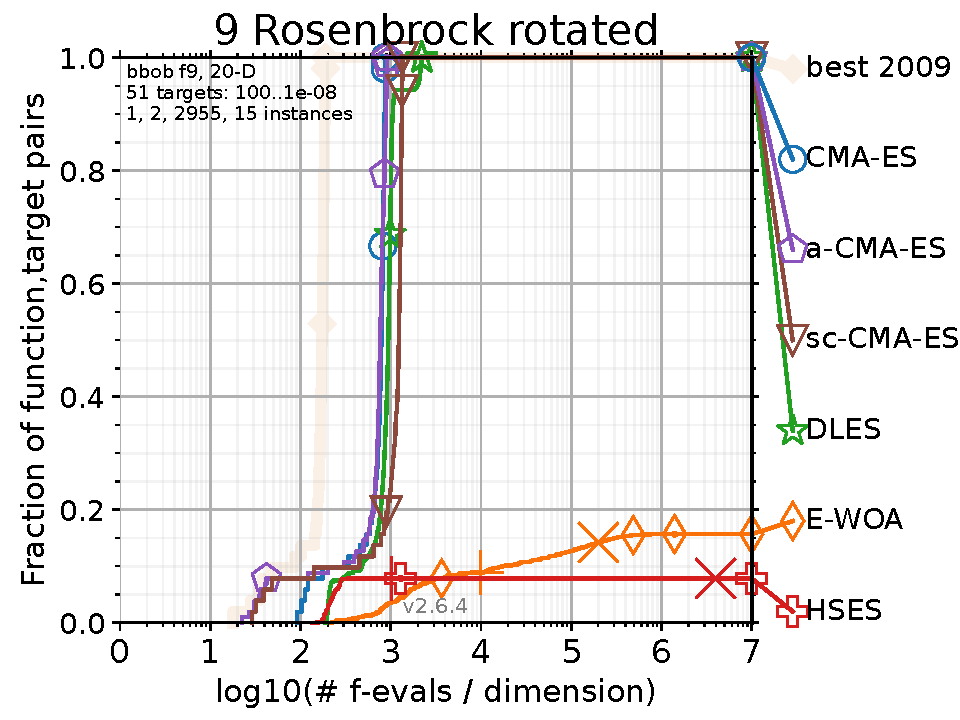
\includegraphics[width=\textwidth]{./bbob/pprldmany_f009_20D.pdf}
	\end{minipage}
	\caption{\textcolor{blue}{F7 to F9 in $D$ = 20.}}
\end{figure}

% 第四组图像
\begin{figure}[H]
	\centering
	\begin{minipage}[b]{0.32\textwidth}
		\centering
		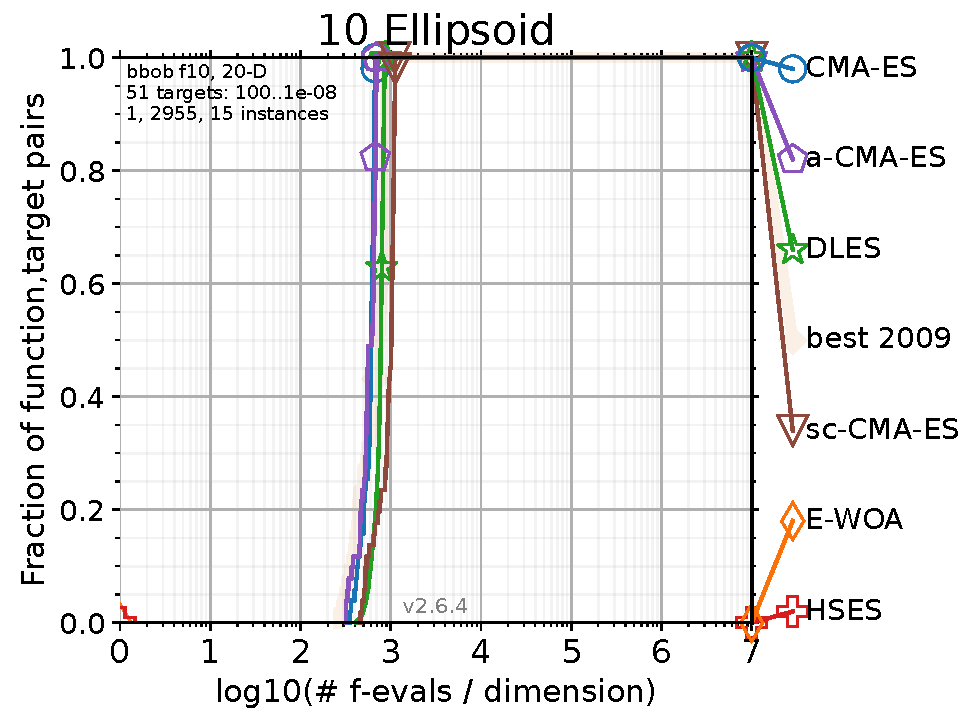
\includegraphics[width=\textwidth]{./bbob/pprldmany_f010_20D.pdf}
	\end{minipage}\hfill
	\begin{minipage}[b]{0.32\textwidth}
		\centering
		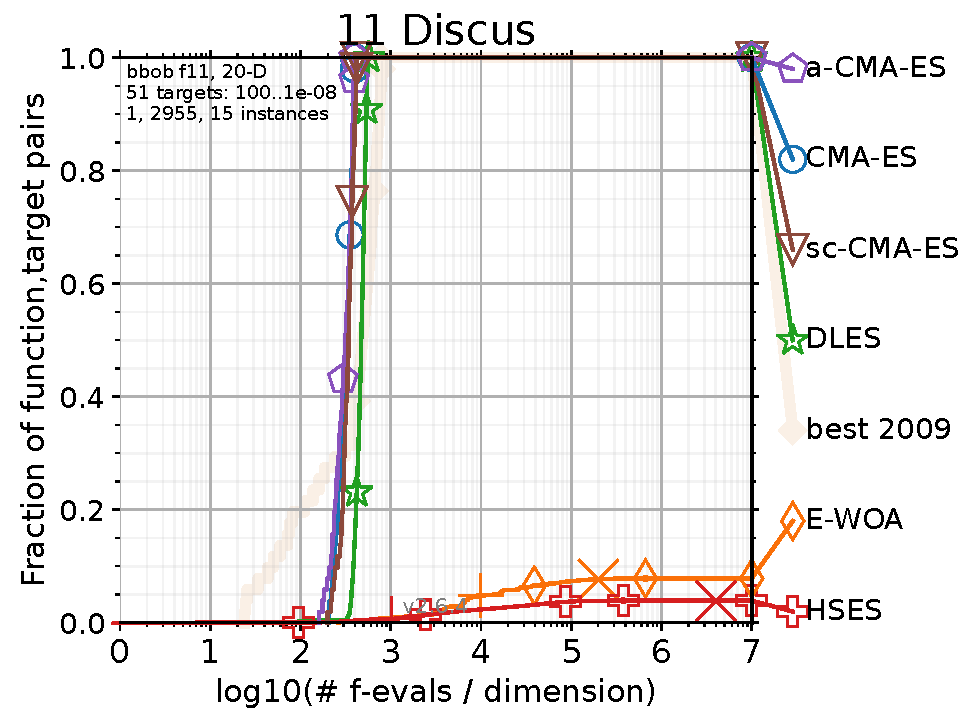
\includegraphics[width=\textwidth]{./bbob/pprldmany_f011_20D.pdf}
	\end{minipage}\hfill
	\begin{minipage}[b]{0.32\textwidth}
		\centering
		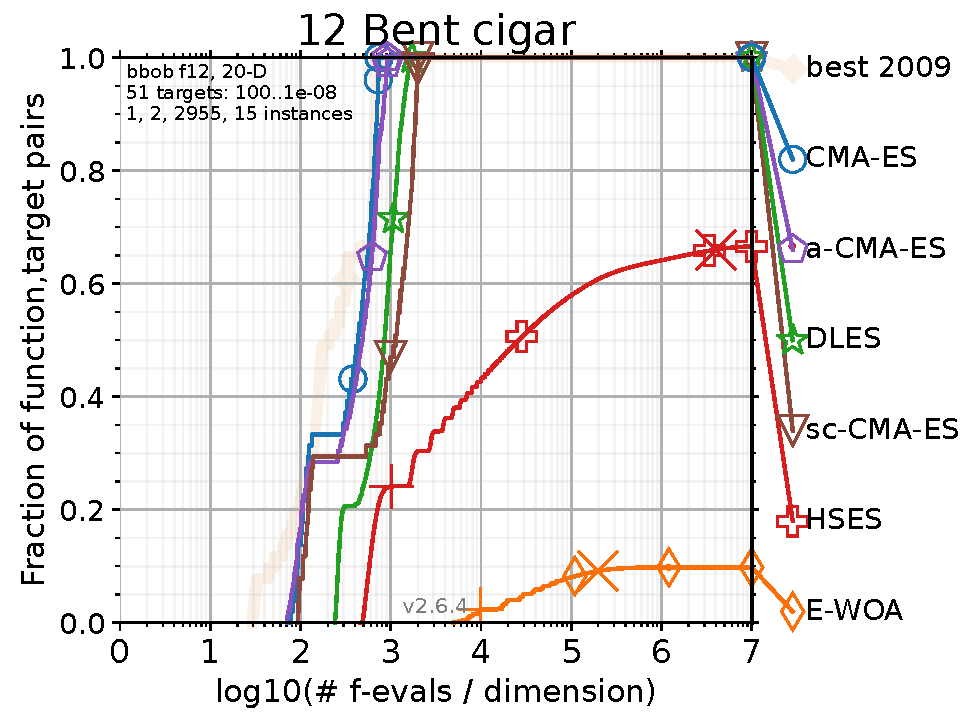
\includegraphics[width=\textwidth]{./bbob/pprldmany_f012_20D.pdf}
	\end{minipage}
	\caption{\textcolor{blue}{F10 to F12 in $D$ = 20.}}
\end{figure}

% 第五组图像
\begin{figure}[H]
	\centering
	\begin{minipage}[b]{0.32\textwidth}
		\centering
		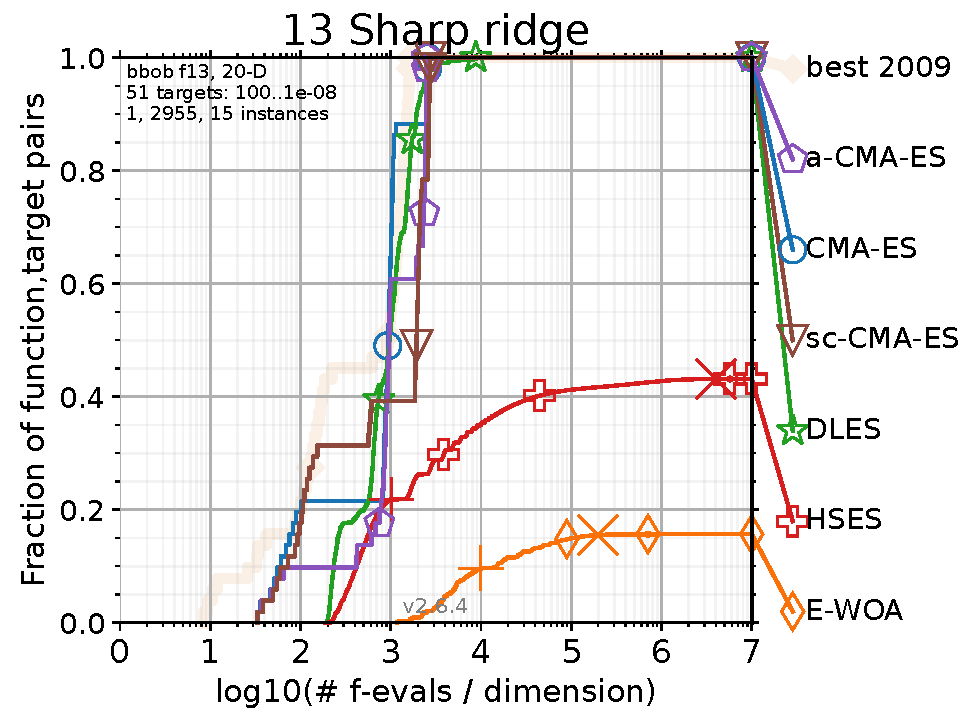
\includegraphics[width=\textwidth]{./bbob/pprldmany_f013_20D.pdf}
	\end{minipage}\hfill
	\begin{minipage}[b]{0.32\textwidth}
		\centering
		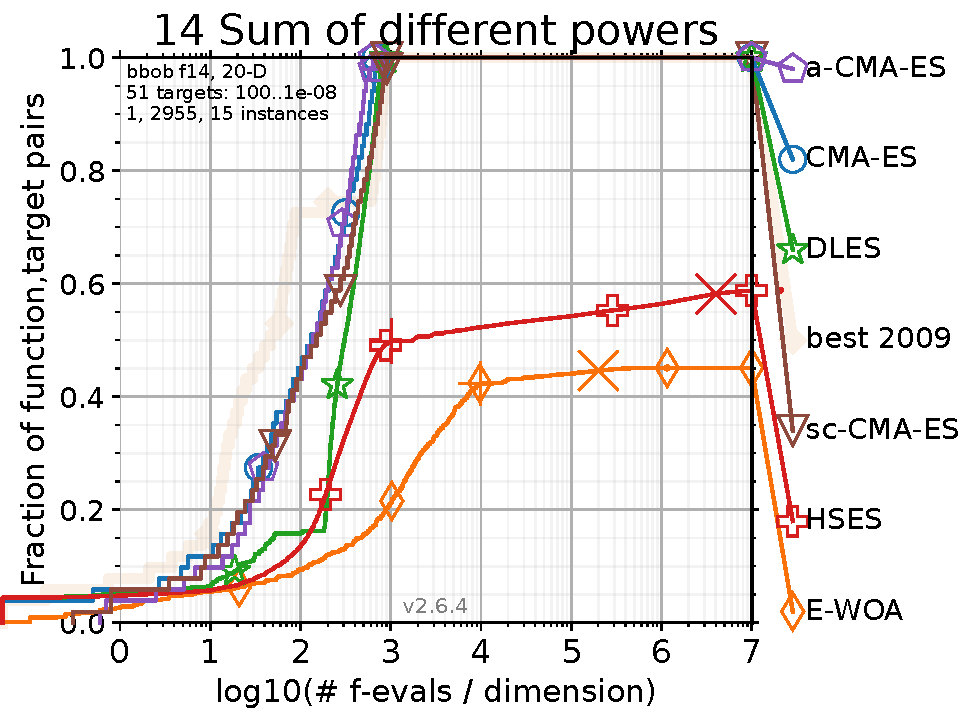
\includegraphics[width=\textwidth]{./bbob/pprldmany_f014_20D.pdf}
	\end{minipage}\hfill
	\begin{minipage}[b]{0.32\textwidth}
		\centering
		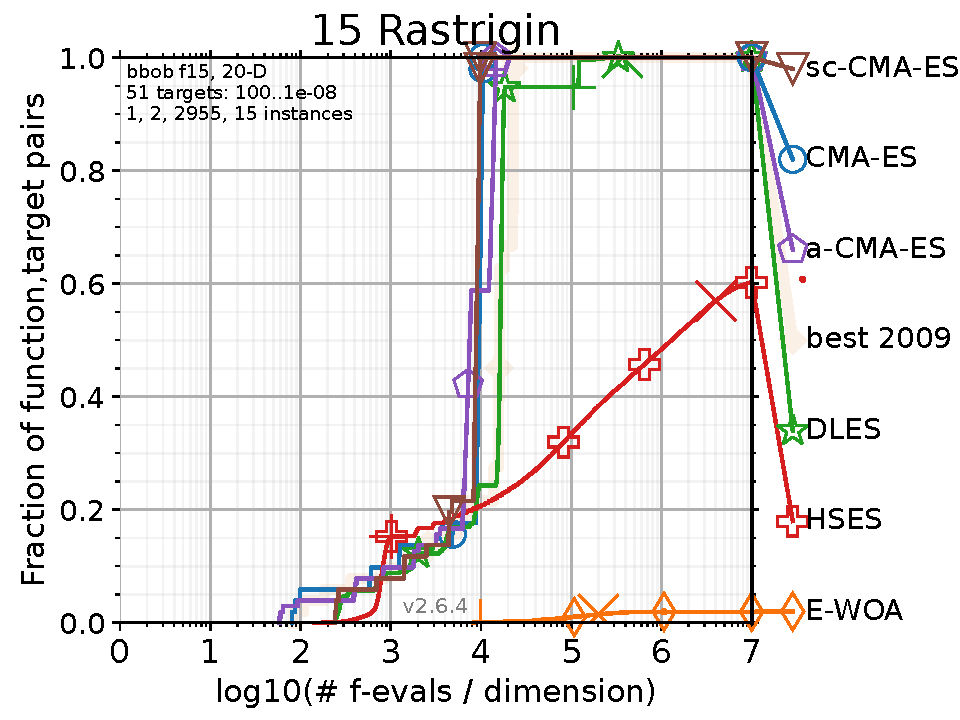
\includegraphics[width=\textwidth]{./bbob/pprldmany_f015_20D.pdf}
	\end{minipage}
	\caption{\textcolor{blue}{F13 to F15 in $D$ = 20.}}
\end{figure}

% 第六组图像
\begin{figure}[H]
	\centering
	\begin{minipage}[b]{0.32\textwidth}
		\centering
		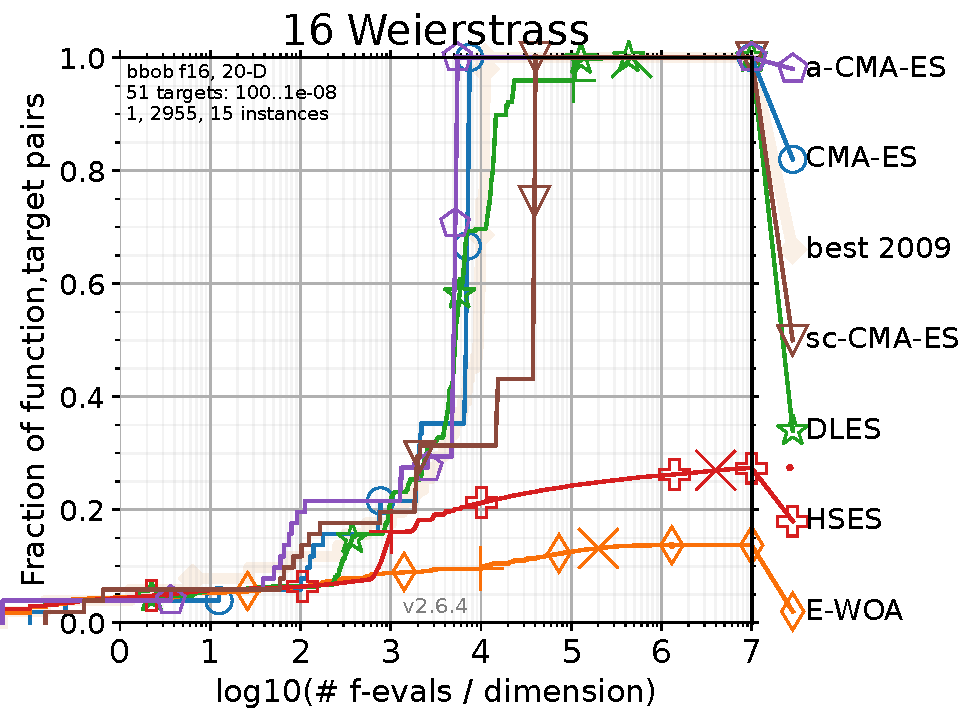
\includegraphics[width=\textwidth]{./bbob/pprldmany_f016_20D.pdf}
	\end{minipage}\hfill
	\begin{minipage}[b]{0.32\textwidth}
		\centering
		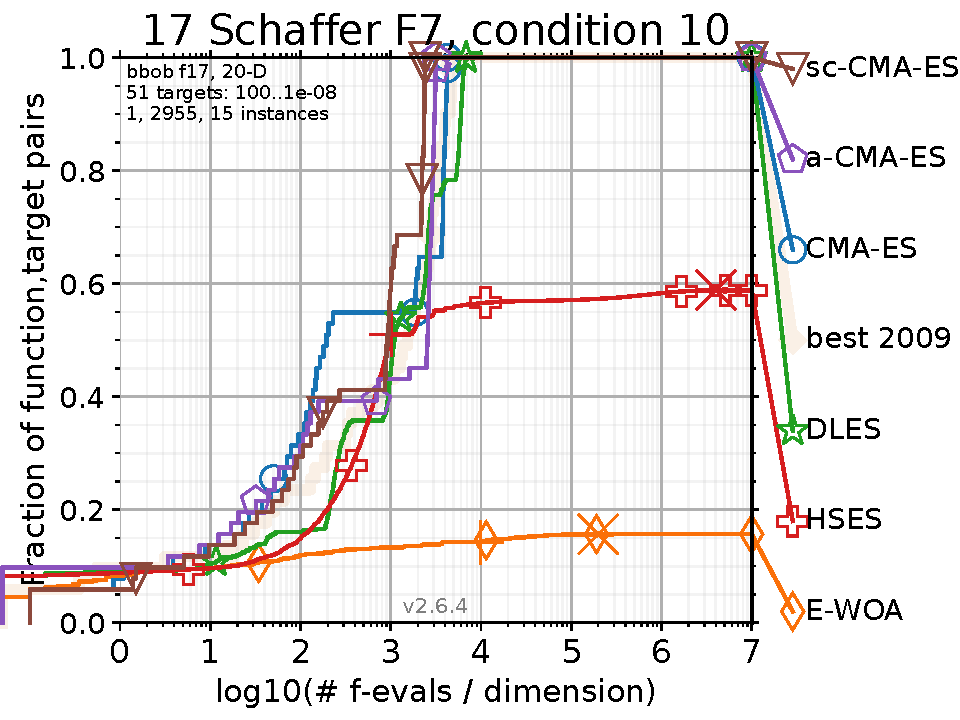
\includegraphics[width=\textwidth]{./bbob/pprldmany_f017_20D.pdf}
	\end{minipage}\hfill
	\begin{minipage}[b]{0.32\textwidth}
		\centering
		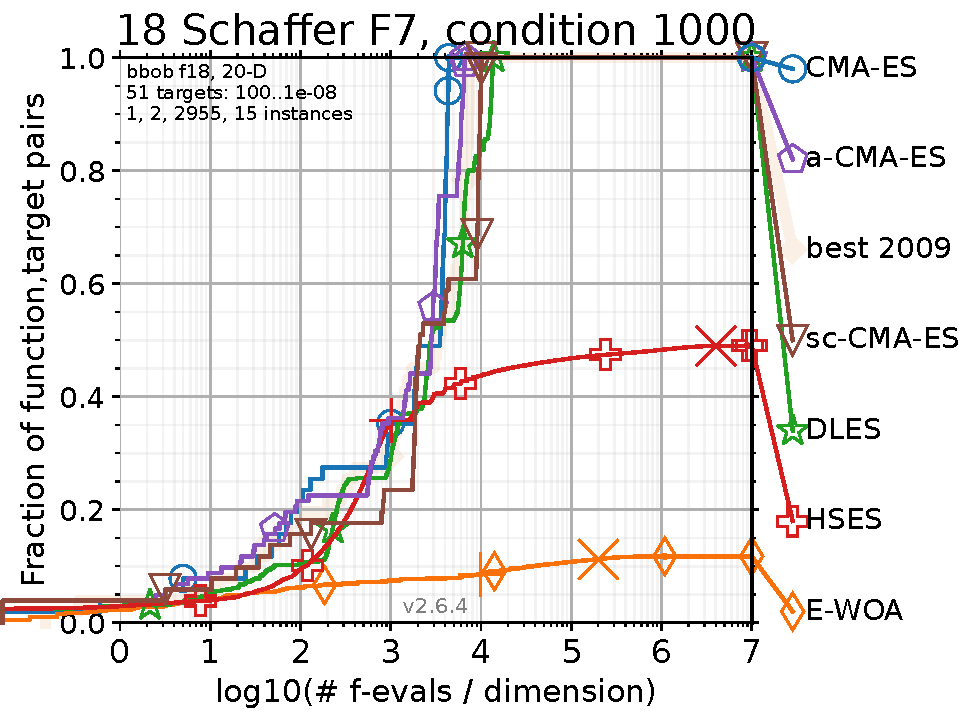
\includegraphics[width=\textwidth]{./bbob/pprldmany_f018_20D.pdf}
	\end{minipage}
	\caption{\textcolor{blue}{F16 to F18 in $D$ = 20.}}
\end{figure}

% 第七组图像
\begin{figure}[H]
	\centering
	\begin{minipage}[b]{0.32\textwidth}
		\centering
		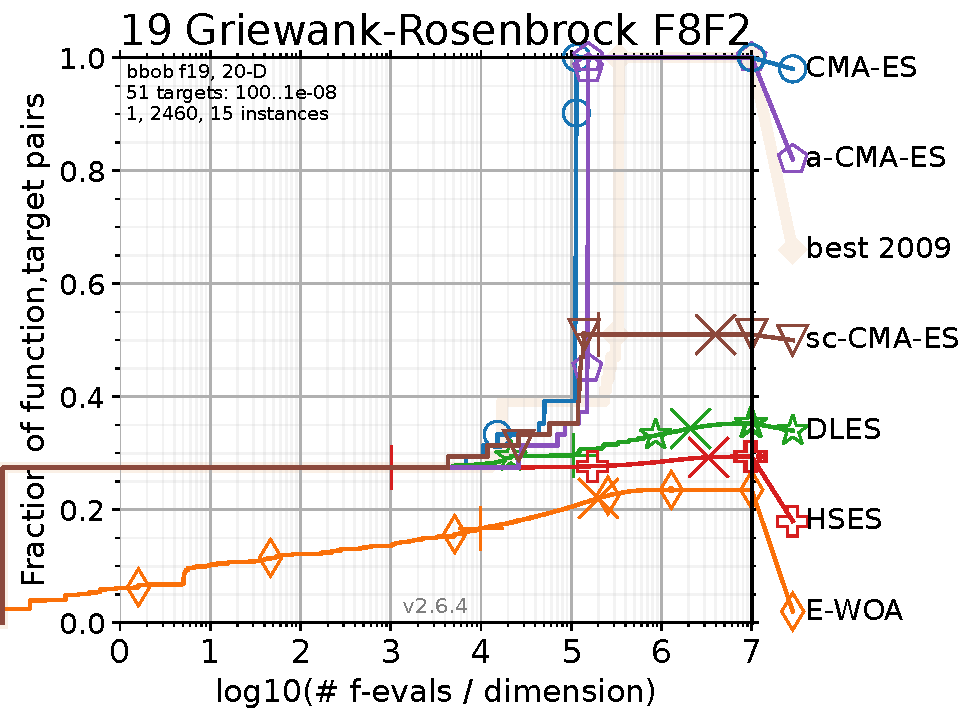
\includegraphics[width=\textwidth]{./bbob/pprldmany_f019_20D.pdf}
	\end{minipage}\hfill
	\begin{minipage}[b]{0.32\textwidth}
		\centering
		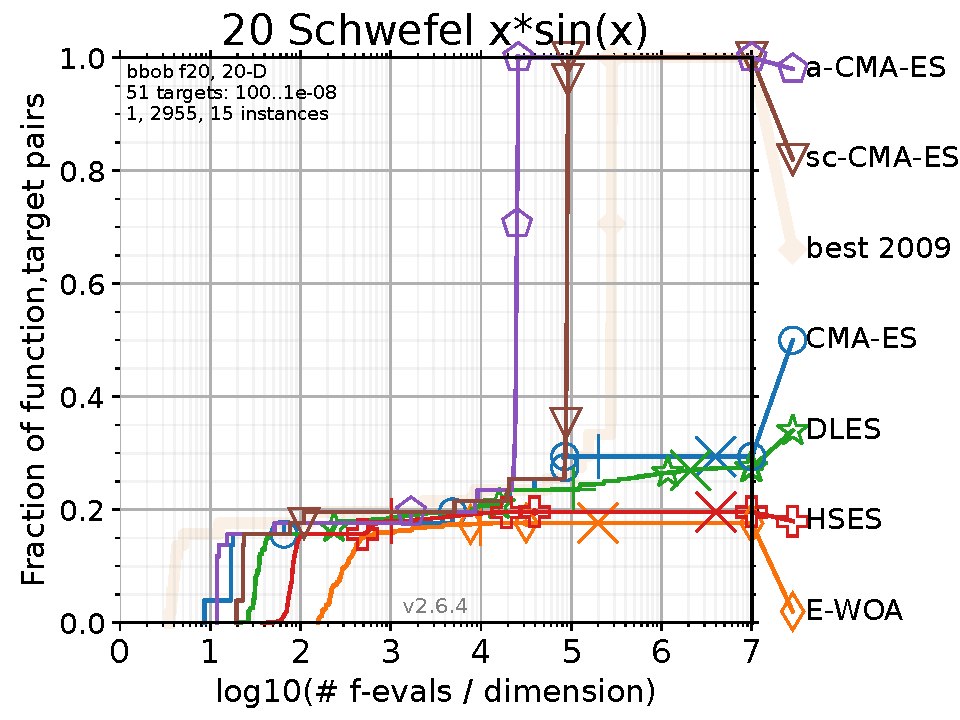
\includegraphics[width=\textwidth]{./bbob/pprldmany_f020_20D.pdf}
	\end{minipage}\hfill
	\begin{minipage}[b]{0.32\textwidth}
		\centering
		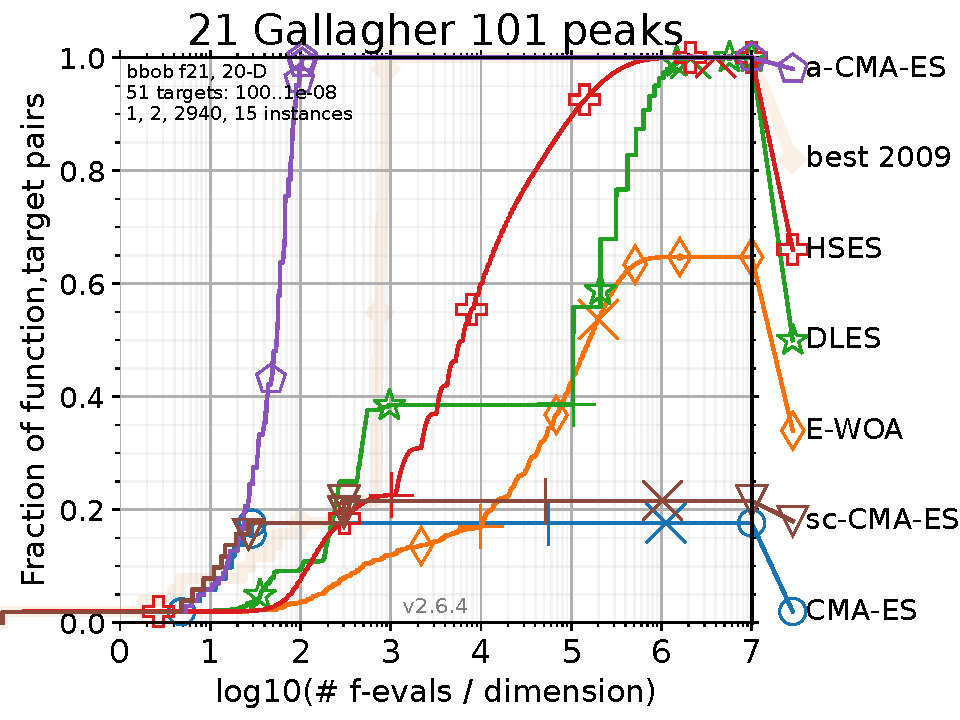
\includegraphics[width=\textwidth]{./bbob/pprldmany_f021_20D.pdf}
	\end{minipage}
	\caption{\textcolor{blue}{F19 to F21 in $D$ = 20.}}
\end{figure}

% 第八组图像
\begin{figure}[H]
	\centering
	\begin{minipage}[b]{0.32\textwidth}
		\centering
		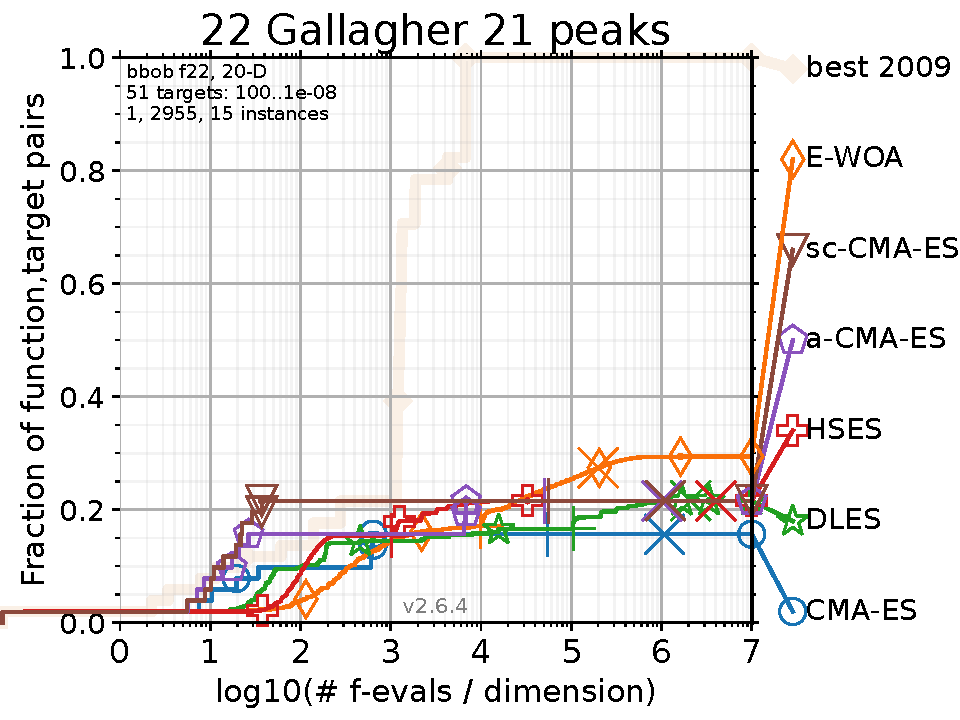
\includegraphics[width=\textwidth]{./bbob/pprldmany_f022_20D.pdf}
	\end{minipage}\hfill
	\begin{minipage}[b]{0.32\textwidth}
		\centering
		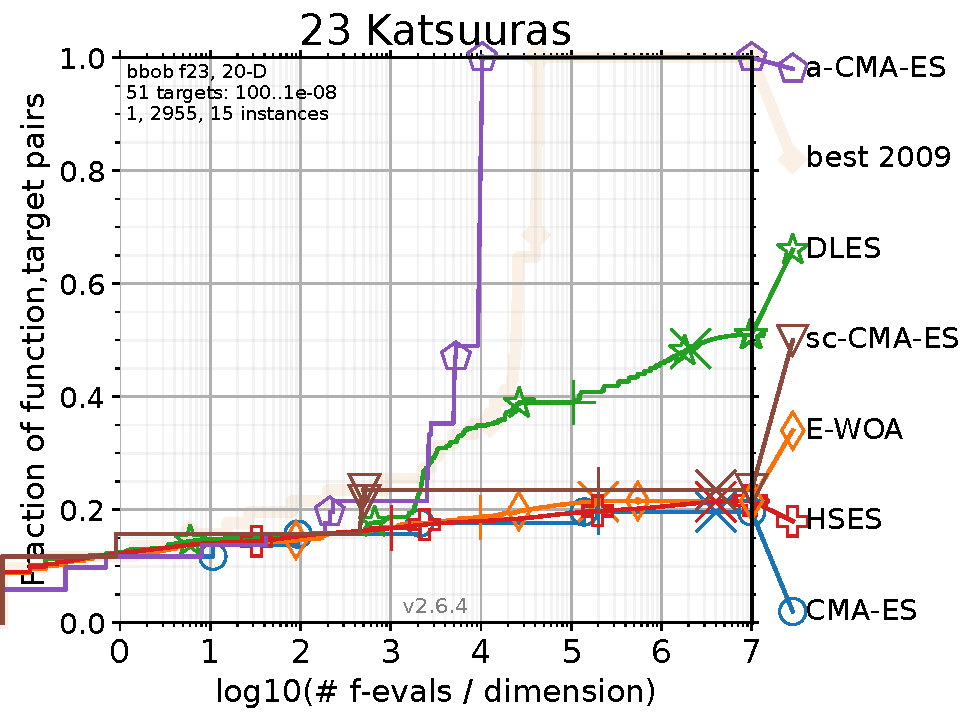
\includegraphics[width=\textwidth]{./bbob/pprldmany_f023_20D.pdf}
	\end{minipage}\hfill
	\begin{minipage}[b]{0.32\textwidth}
		\centering
		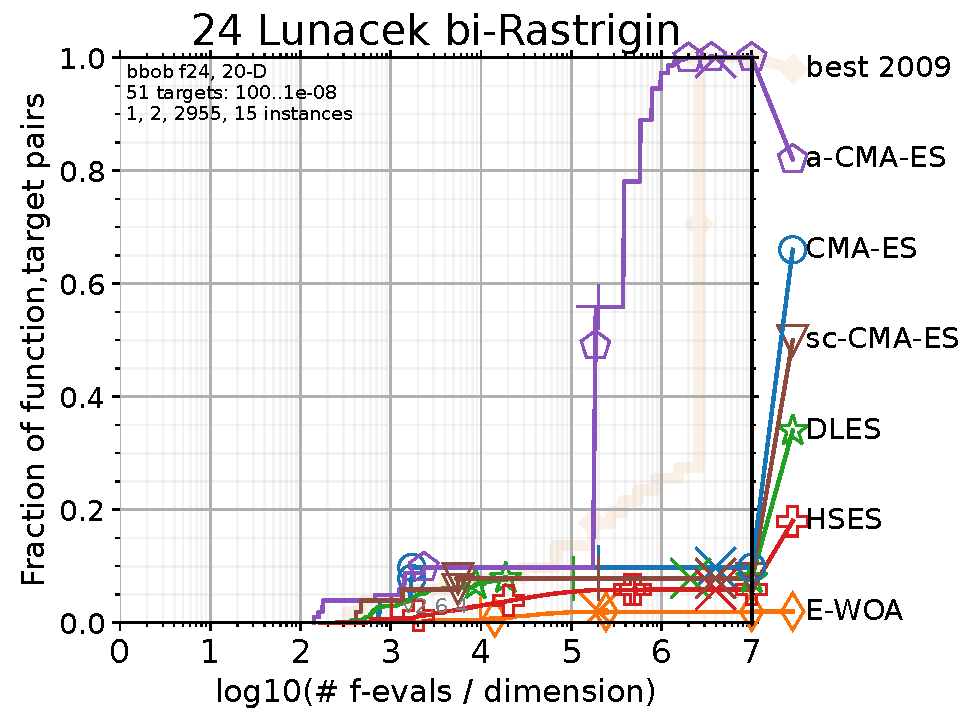
\includegraphics[width=\textwidth]{./bbob/pprldmany_f024_20D.pdf}
	\end{minipage}
	\caption{\textcolor{blue}{F22 to F24 in $D$ = 20.}}
\end{figure}

% 第一组图像
\begin{figure}[H]
	\centering
	\begin{minipage}[b]{0.32\textwidth}
		\centering
		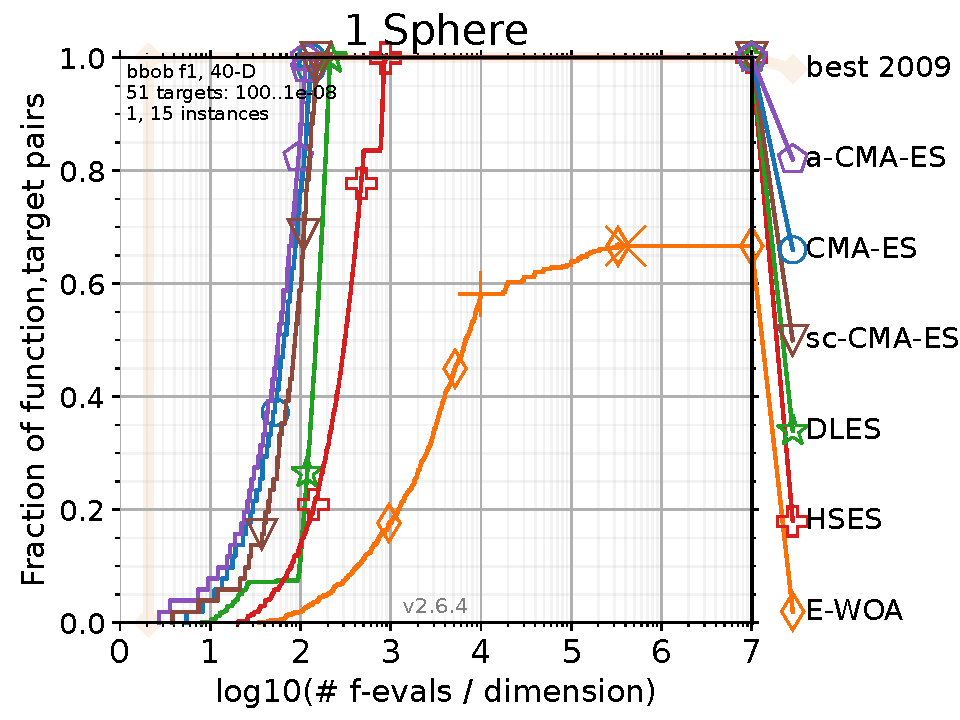
\includegraphics[width=\textwidth]{./bbob/pprldmany_f001_40D.pdf}
	\end{minipage}\hfill
	\begin{minipage}[b]{0.32\textwidth}
		\centering
		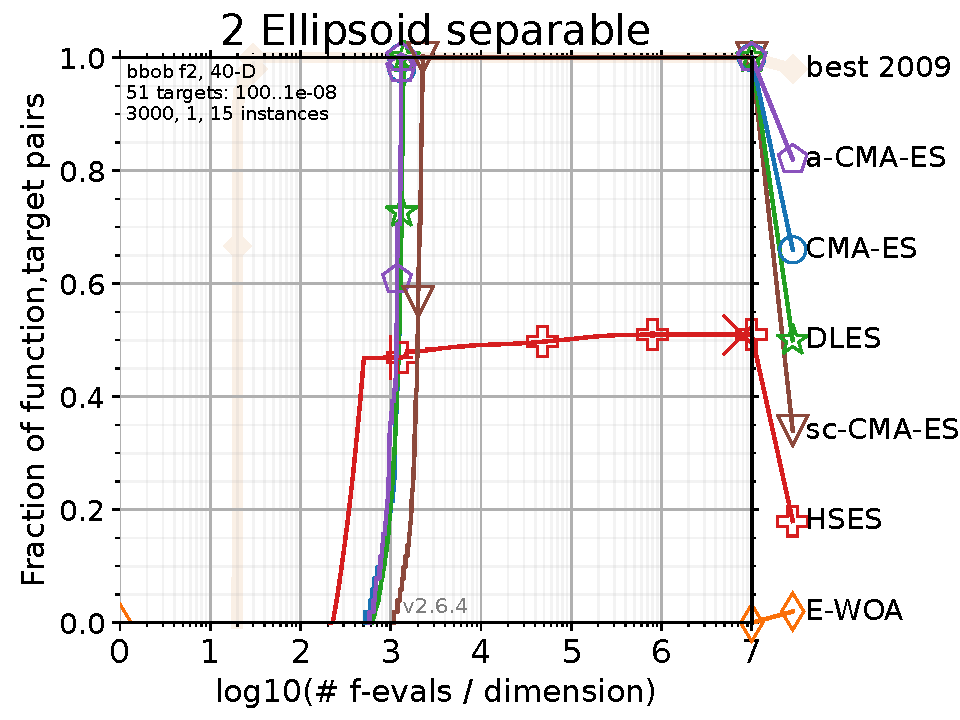
\includegraphics[width=\textwidth]{./bbob/pprldmany_f002_40D.pdf}
	\end{minipage}\hfill
	\begin{minipage}[b]{0.32\textwidth}
		\centering
		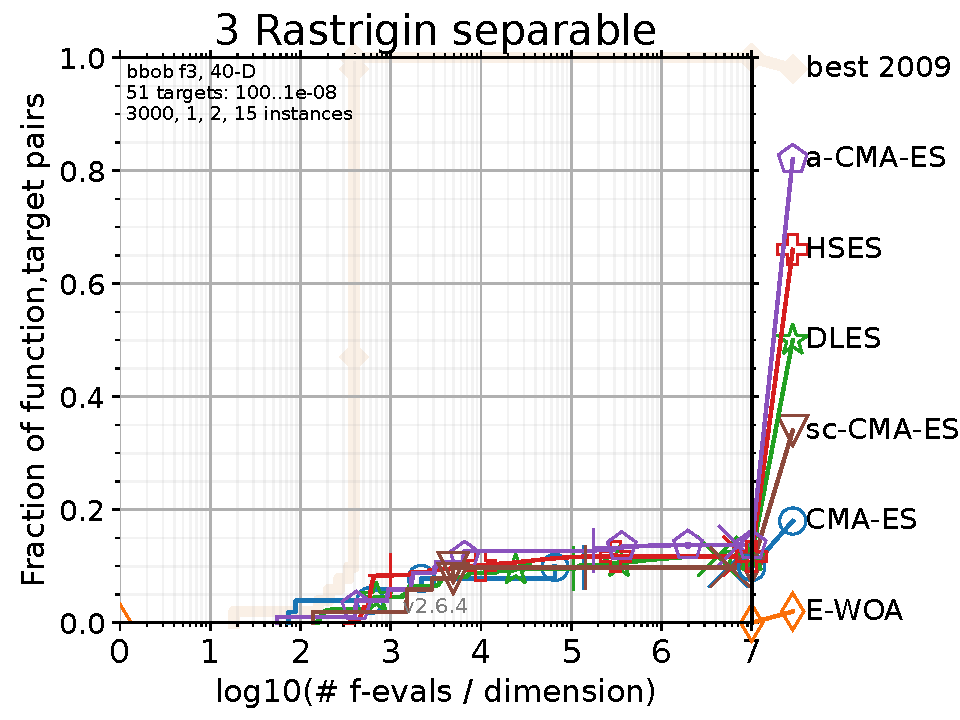
\includegraphics[width=\textwidth]{./bbob/pprldmany_f003_40D.pdf}
	\end{minipage}
	\caption{\textcolor{blue}{F1 to F3 in $D$ = 40.}}
\end{figure}

% 第二组图像
\begin{figure}[H]
	\centering
	\begin{minipage}[b]{0.32\textwidth}
		\centering
		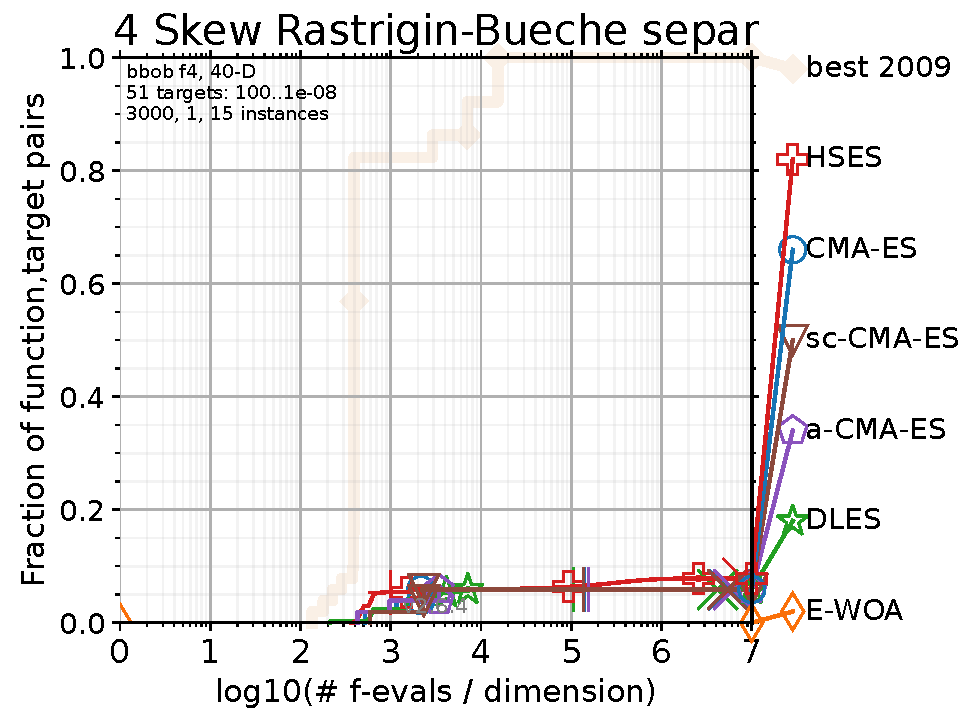
\includegraphics[width=\textwidth]{./bbob/pprldmany_f004_40D.pdf}
	\end{minipage}\hfill
	\begin{minipage}[b]{0.32\textwidth}
		\centering
		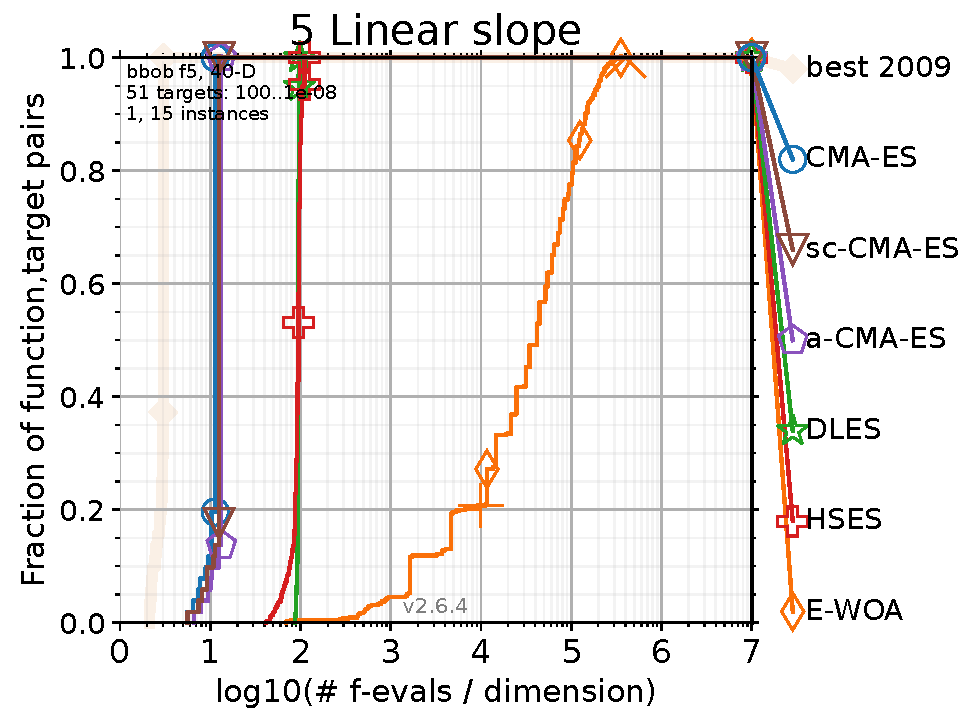
\includegraphics[width=\textwidth]{./bbob/pprldmany_f005_40D.pdf}
	\end{minipage}\hfill
	\begin{minipage}[b]{0.32\textwidth}
		\centering
		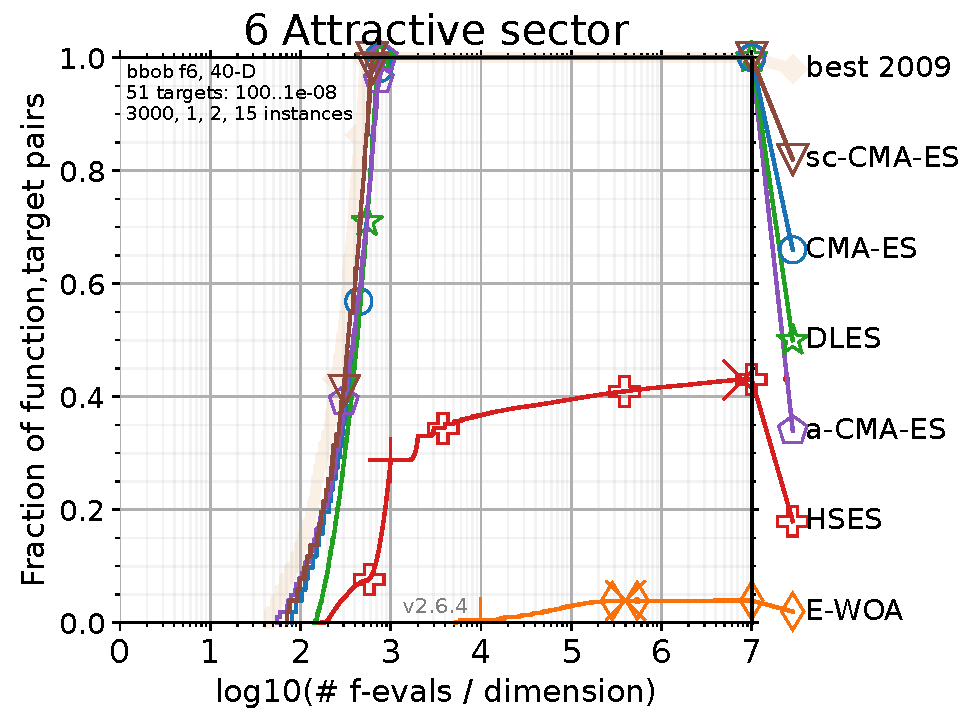
\includegraphics[width=\textwidth]{./bbob/pprldmany_f006_40D.pdf}
	\end{minipage}
	\caption{\textcolor{blue}{F4 to F6 in $D$ = 40.}}
\end{figure}

% 第三组图像
\begin{figure}[H]
	\centering
	\begin{minipage}[b]{0.32\textwidth}
		\centering
		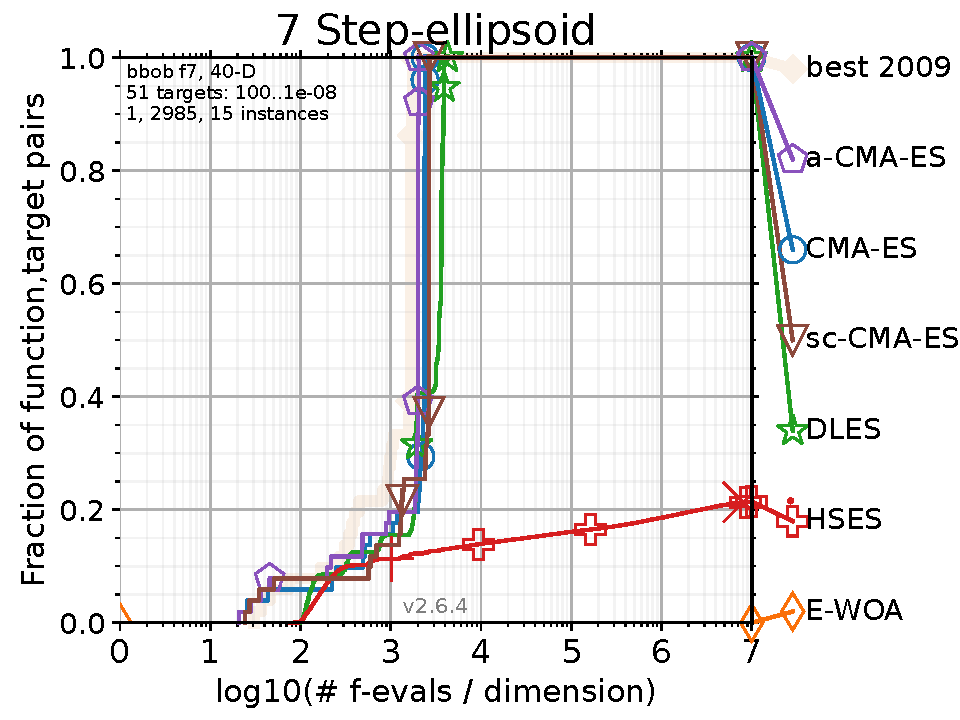
\includegraphics[width=\textwidth]{./bbob/pprldmany_f007_40D.pdf}
	\end{minipage}\hfill
	\begin{minipage}[b]{0.32\textwidth}
		\centering
		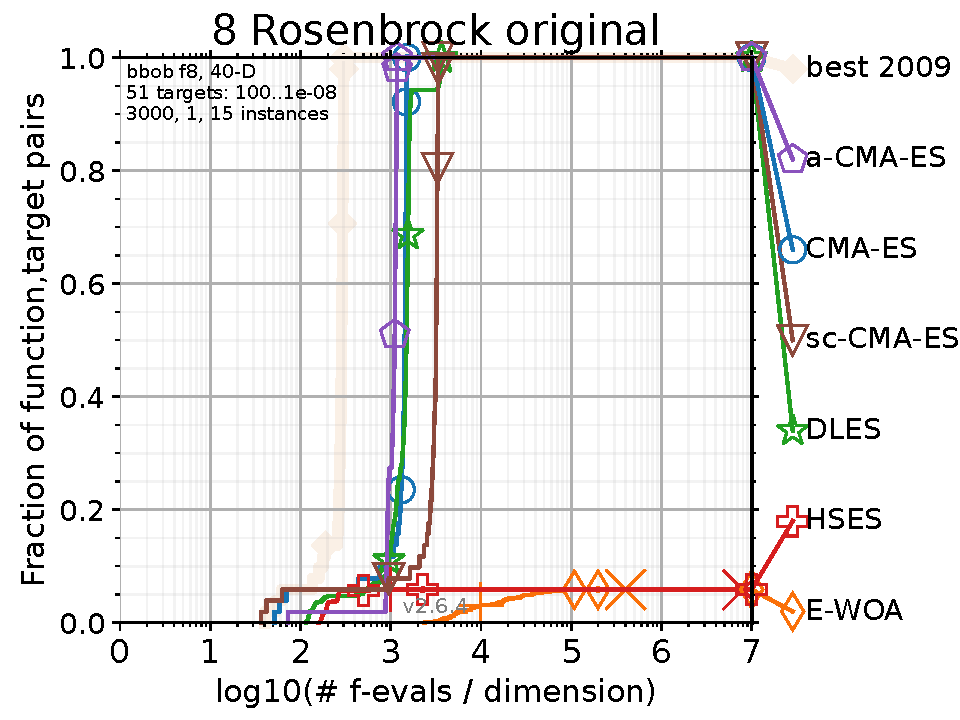
\includegraphics[width=\textwidth]{./bbob/pprldmany_f008_40D.pdf}
	\end{minipage}\hfill
	\begin{minipage}[b]{0.32\textwidth}
		\centering
		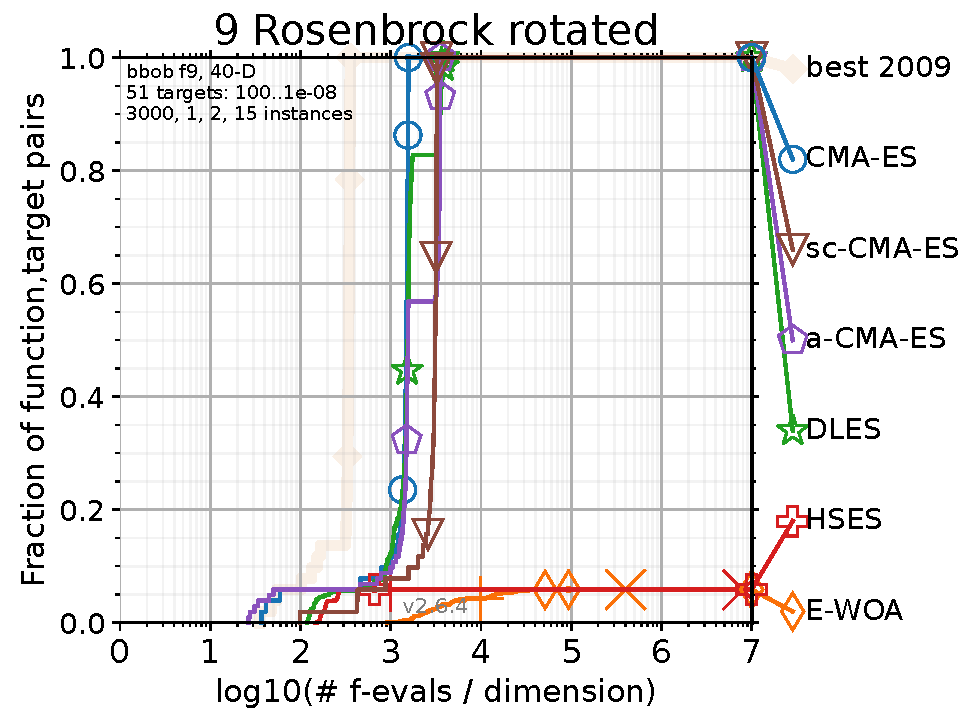
\includegraphics[width=\textwidth]{./bbob/pprldmany_f009_40D.pdf}
	\end{minipage}
	\caption{\textcolor{blue}{F7 to F9 in $D$ = 40.}}
\end{figure}

% 第四组图像
\begin{figure}[H]
	\centering
	\begin{minipage}[b]{0.32\textwidth}
		\centering
		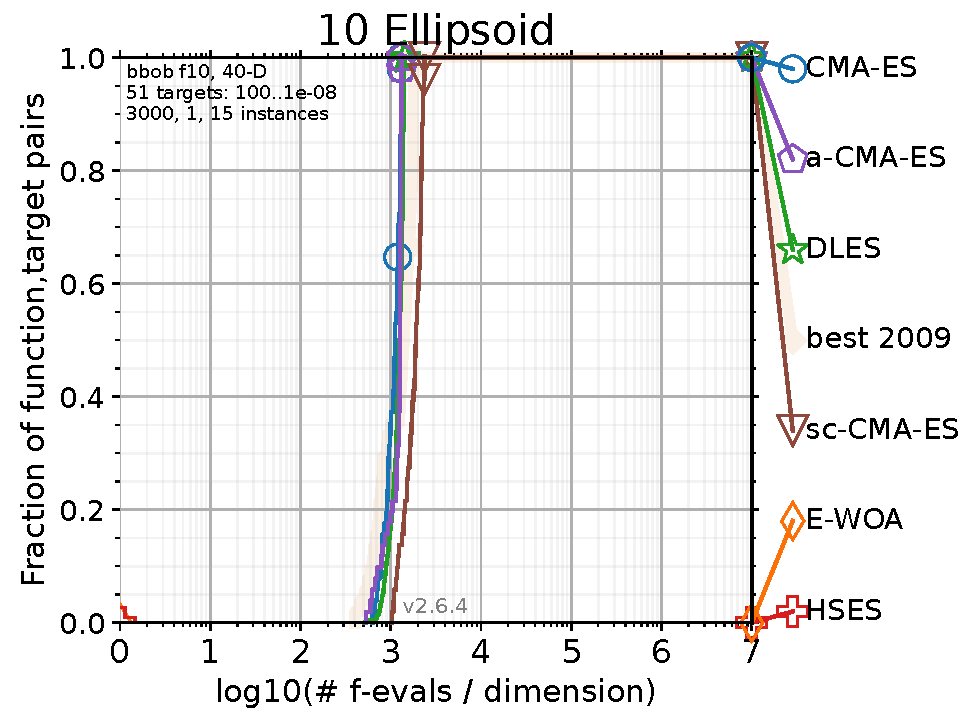
\includegraphics[width=\textwidth]{./bbob/pprldmany_f010_40D.pdf}
	\end{minipage}\hfill
	\begin{minipage}[b]{0.32\textwidth}
		\centering
		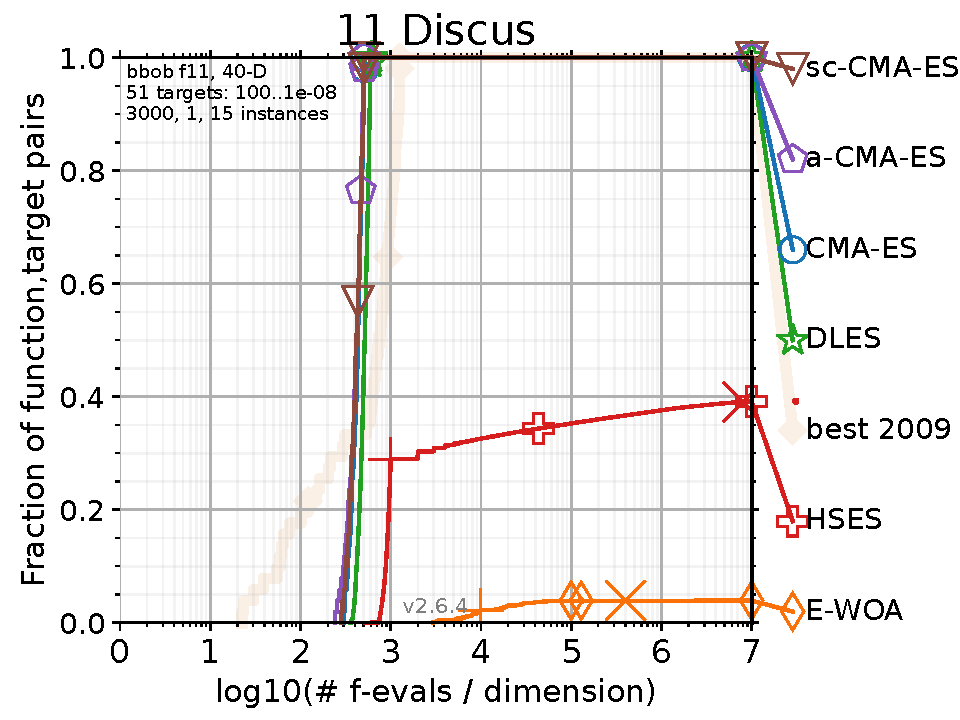
\includegraphics[width=\textwidth]{./bbob/pprldmany_f011_40D.pdf}
	\end{minipage}\hfill
	\begin{minipage}[b]{0.32\textwidth}
		\centering
		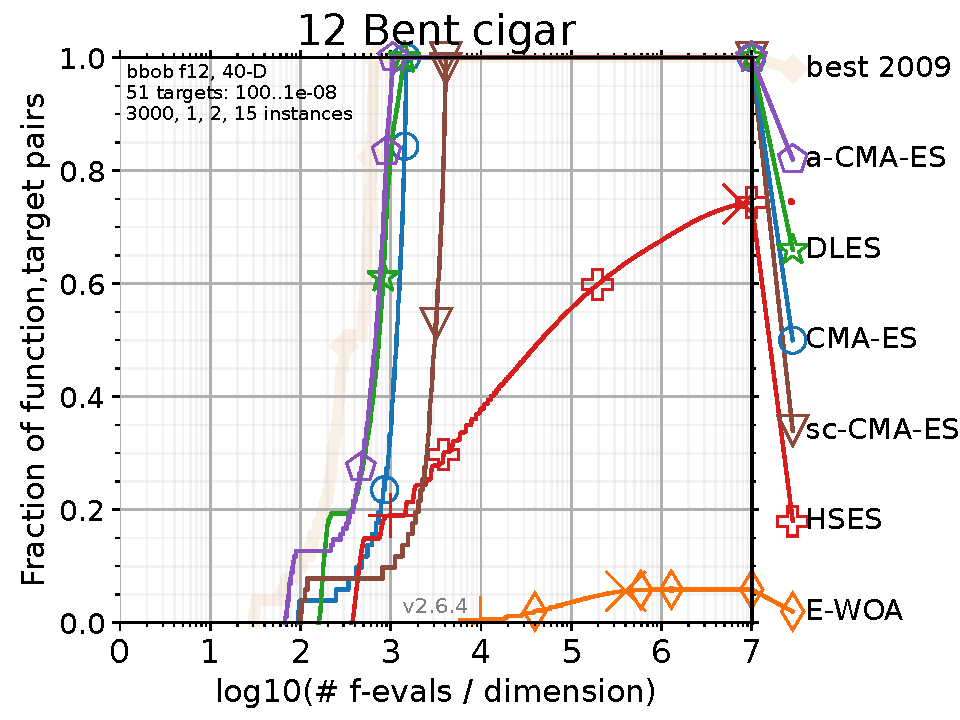
\includegraphics[width=\textwidth]{./bbob/pprldmany_f012_40D.pdf}
	\end{minipage}
	\caption{\textcolor{blue}{F10 to F12 in $D$ = 40.}}
\end{figure}

% 第五组图像
\begin{figure}[H]
	\centering
	\begin{minipage}[b]{0.32\textwidth}
		\centering
		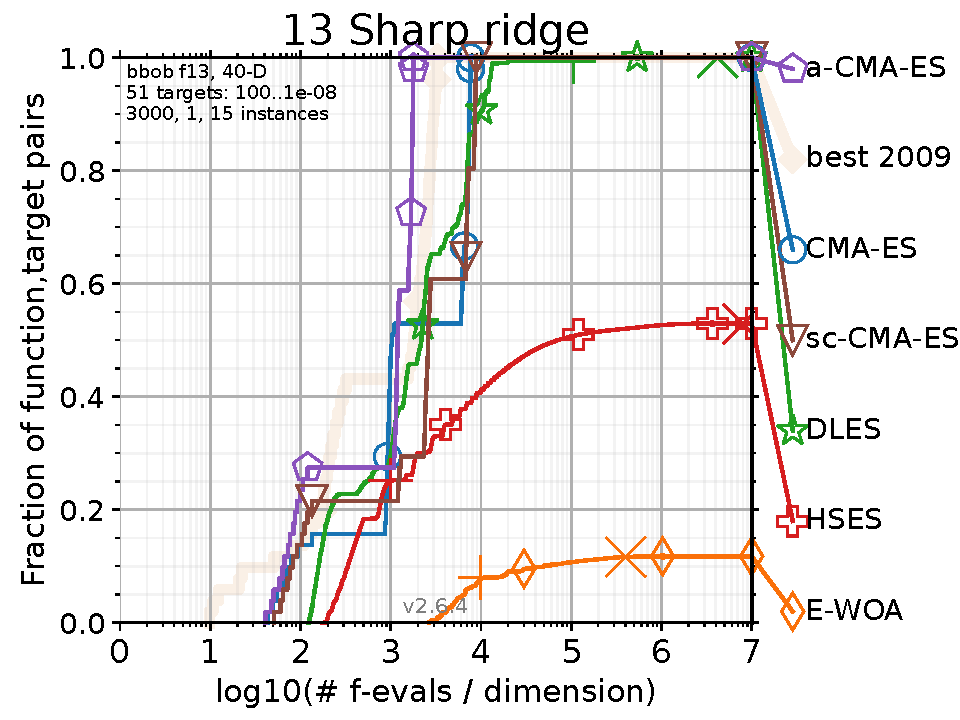
\includegraphics[width=\textwidth]{./bbob/pprldmany_f013_40D.pdf}
	\end{minipage}\hfill
	\begin{minipage}[b]{0.32\textwidth}
		\centering
		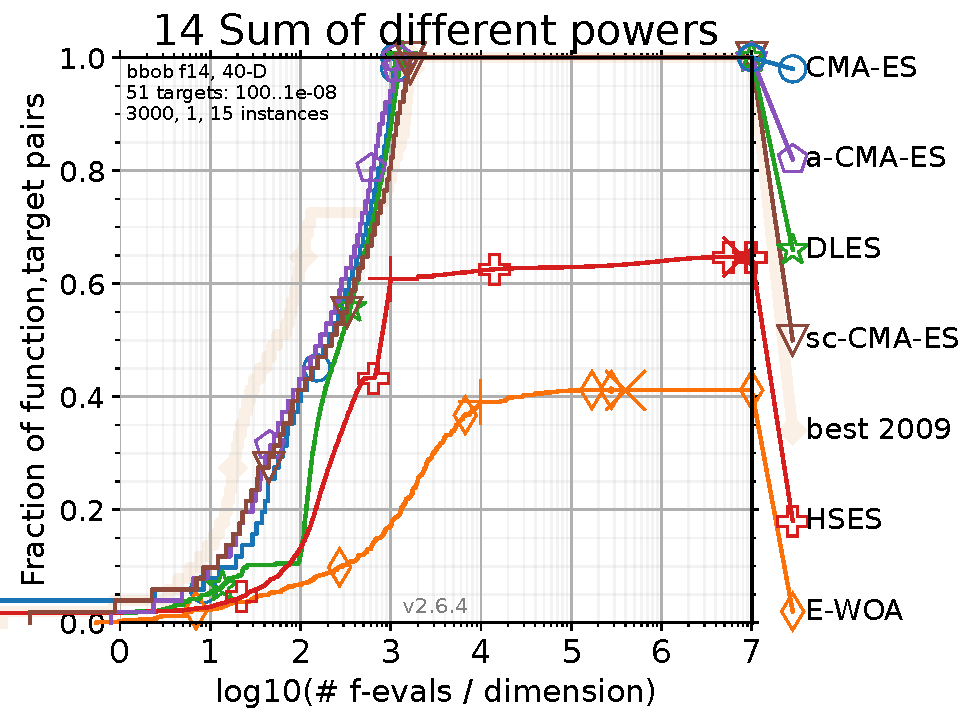
\includegraphics[width=\textwidth]{./bbob/pprldmany_f014_40D.pdf}
	\end{minipage}\hfill
	\begin{minipage}[b]{0.32\textwidth}
		\centering
		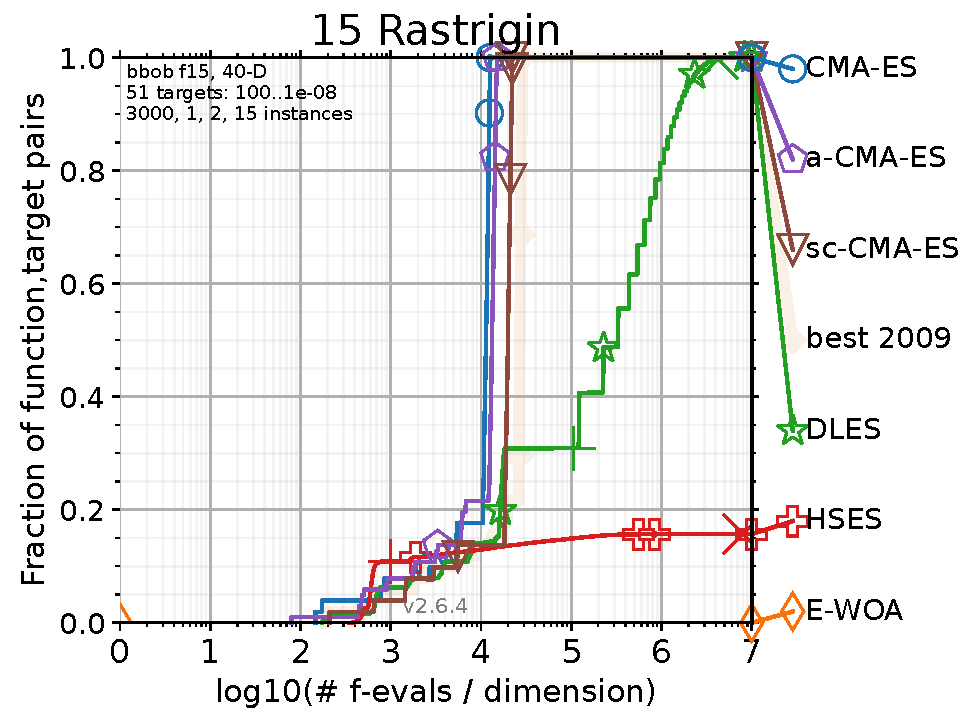
\includegraphics[width=\textwidth]{./bbob/pprldmany_f015_40D.pdf}
	\end{minipage}
	\caption{\textcolor{blue}{F13 to F15 in $D$ = 40.}}
\end{figure}

% 第六组图像
\begin{figure}[H]
	\centering
	\begin{minipage}[b]{0.32\textwidth}
		\centering
		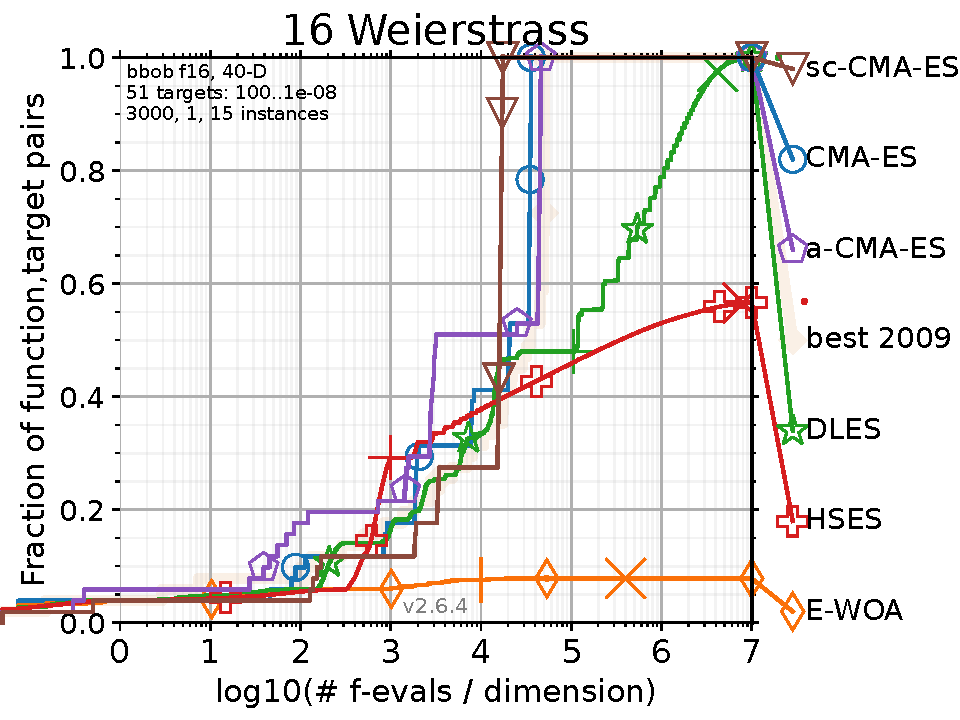
\includegraphics[width=\textwidth]{./bbob/pprldmany_f016_40D.pdf}
	\end{minipage}\hfill
	\begin{minipage}[b]{0.32\textwidth}
		\centering
		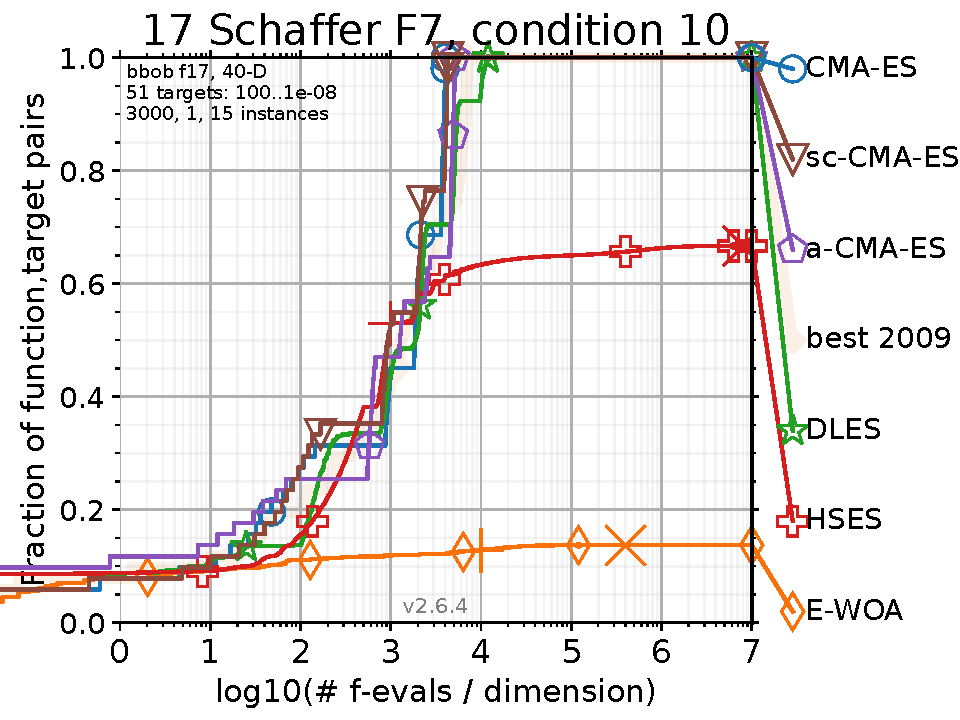
\includegraphics[width=\textwidth]{./bbob/pprldmany_f017_40D.pdf}
	\end{minipage}\hfill
	\begin{minipage}[b]{0.32\textwidth}
		\centering
		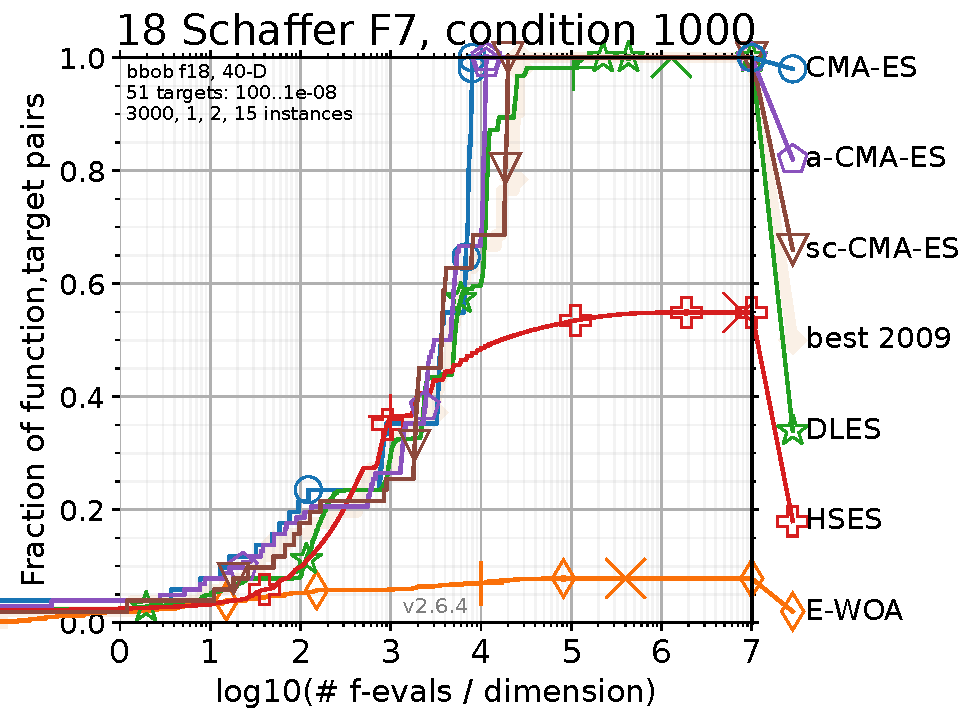
\includegraphics[width=\textwidth]{./bbob/pprldmany_f018_40D.pdf}
	\end{minipage}
	\caption{\textcolor{blue}{F16 to F18 in $D$ = 40.}}
\end{figure}

% 第七组图像
\begin{figure}[H]
	\centering
	\begin{minipage}[b]{0.32\textwidth}
		\centering
		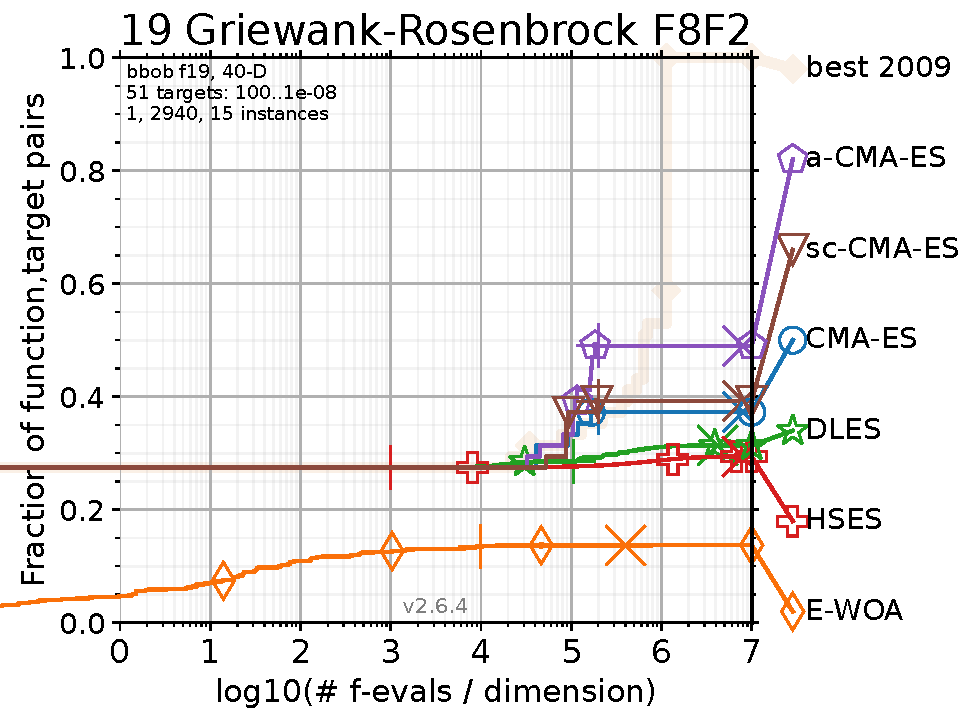
\includegraphics[width=\textwidth]{./bbob/pprldmany_f019_40D.pdf}
	\end{minipage}\hfill
	\begin{minipage}[b]{0.32\textwidth}
		\centering
		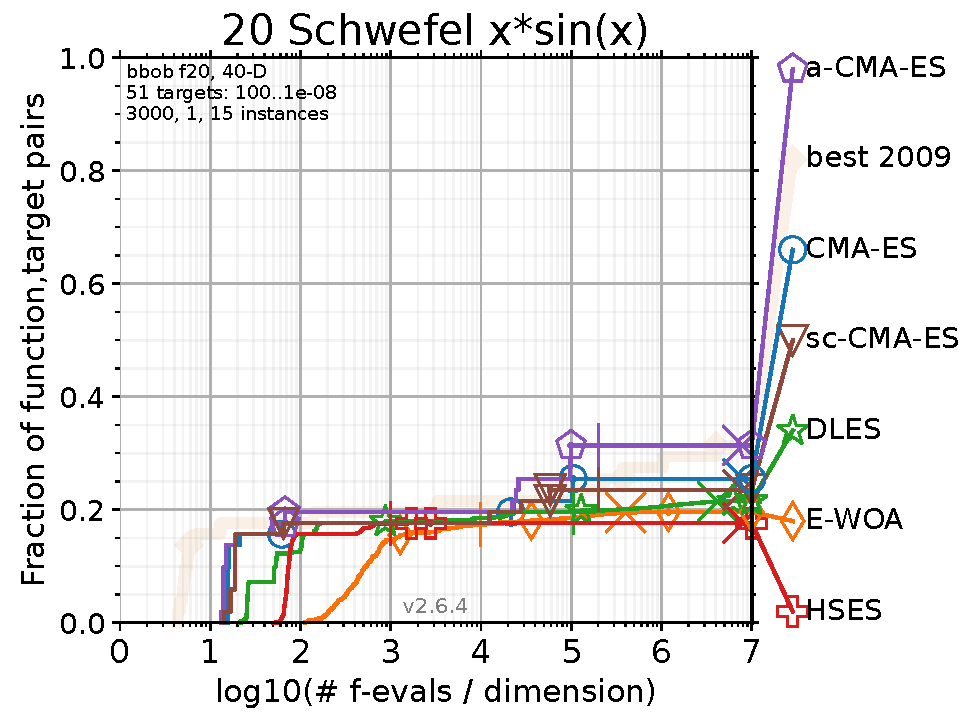
\includegraphics[width=\textwidth]{./bbob/pprldmany_f020_40D.pdf}
	\end{minipage}\hfill
	\begin{minipage}[b]{0.32\textwidth}
		\centering
		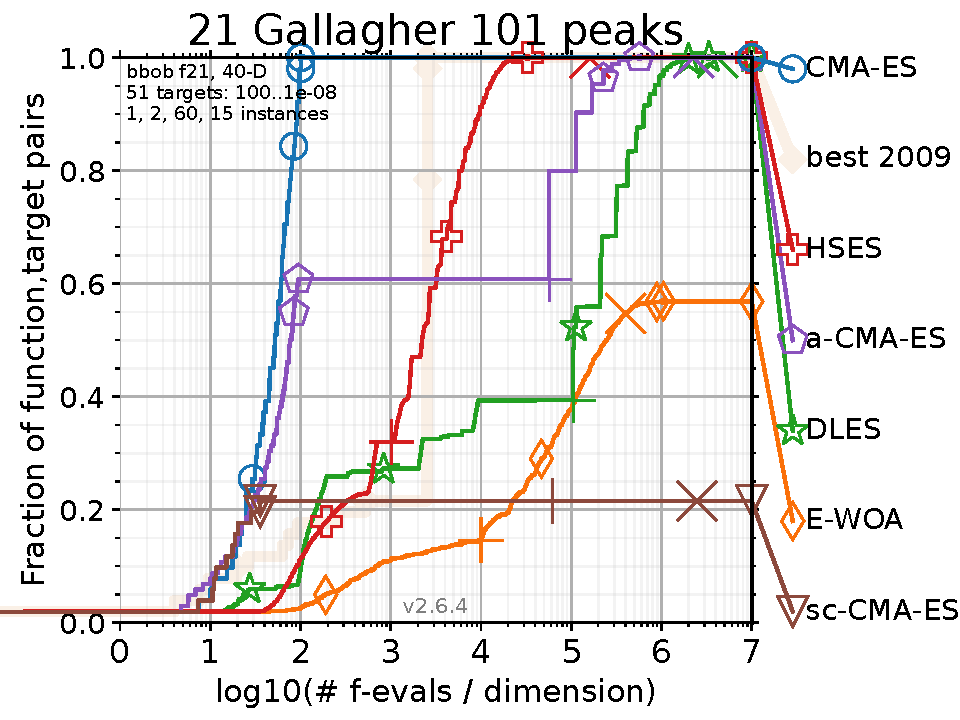
\includegraphics[width=\textwidth]{./bbob/pprldmany_f021_40D.pdf}
	\end{minipage}
	\caption{\textcolor{blue}{F19 to F21 in $D$ = 40.}}
\end{figure}

% 第八组图像
\begin{figure}[H]
	\centering
	\begin{minipage}[b]{0.32\textwidth}
		\centering
		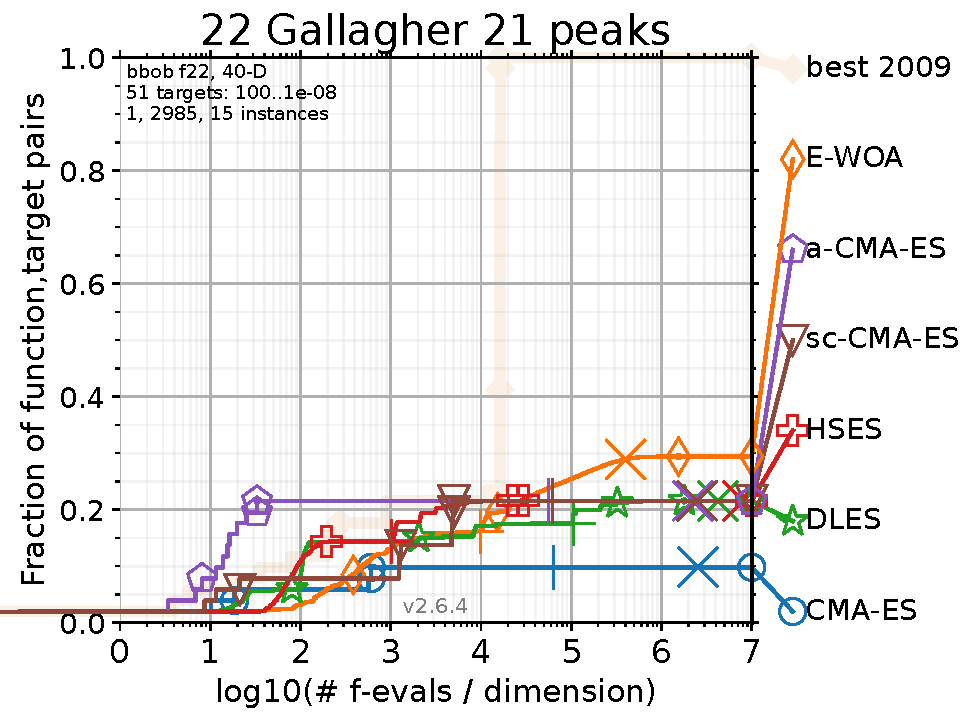
\includegraphics[width=\textwidth]{./bbob/pprldmany_f022_40D.pdf}
	\end{minipage}\hfill
	\begin{minipage}[b]{0.32\textwidth}
		\centering
		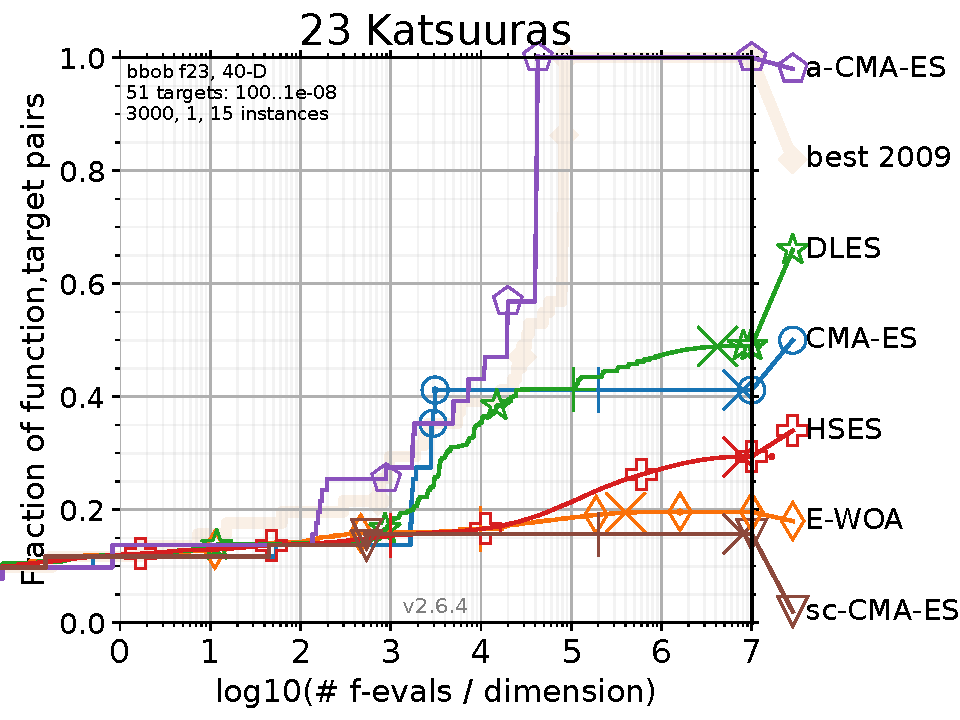
\includegraphics[width=\textwidth]{./bbob/pprldmany_f023_40D.pdf}
	\end{minipage}\hfill
	\begin{minipage}[b]{0.32\textwidth}
		\centering
		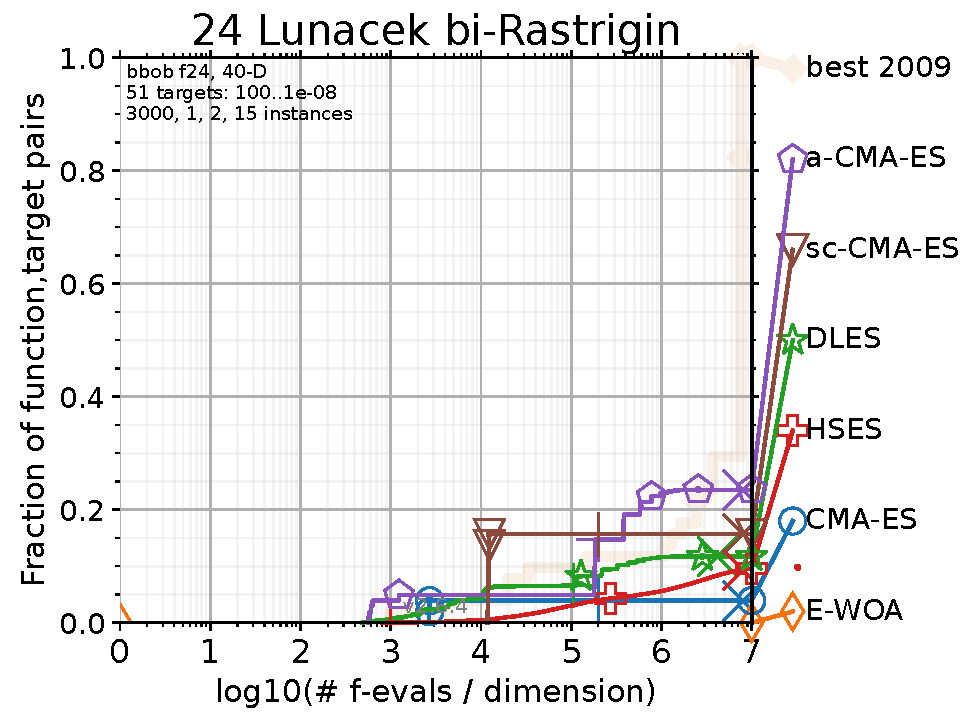
\includegraphics[width=\textwidth]{./bbob/pprldmany_f024_40D.pdf}
	\end{minipage}
	\caption{\textcolor{blue}{F22 to F24 in $D$ = 40.}}
	\label{bbob-end}
\end{figure}

%---------------------------------------CEC 2018 -------------------------------
% 第一组图像
\begin{figure}[H]
	\centering
	\begin{minipage}[b]{0.3\textwidth}
		\centering
		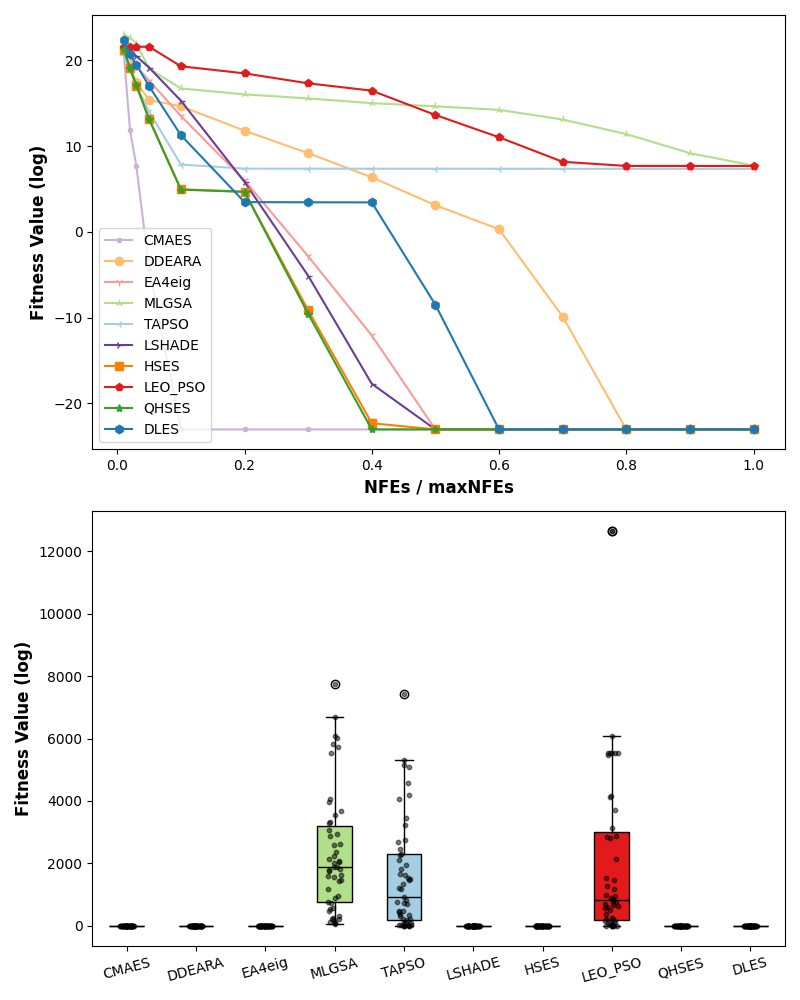
\includegraphics[width=\textwidth]{./save/D_10_F_1.png}
	\end{minipage}\hfill
	\begin{minipage}[b]{0.3\textwidth}
		\centering
		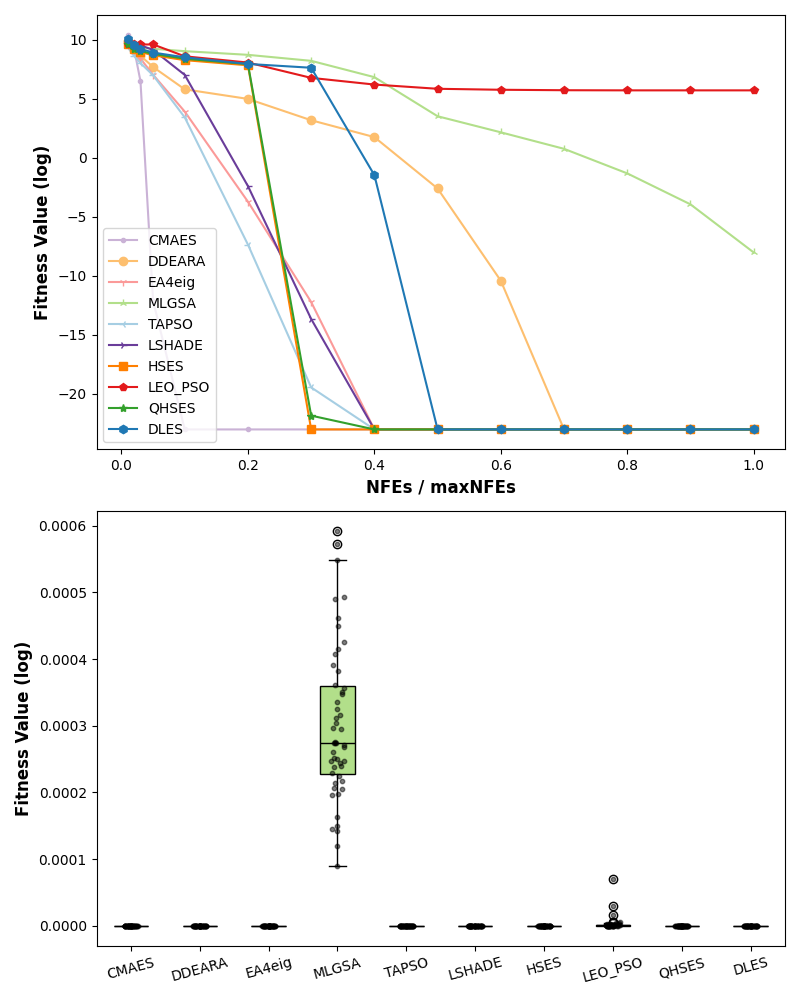
\includegraphics[width=\textwidth]{./save/D_10_F_3.png}
	\end{minipage}\hfill
	\begin{minipage}[b]{0.3\textwidth}
		\centering
		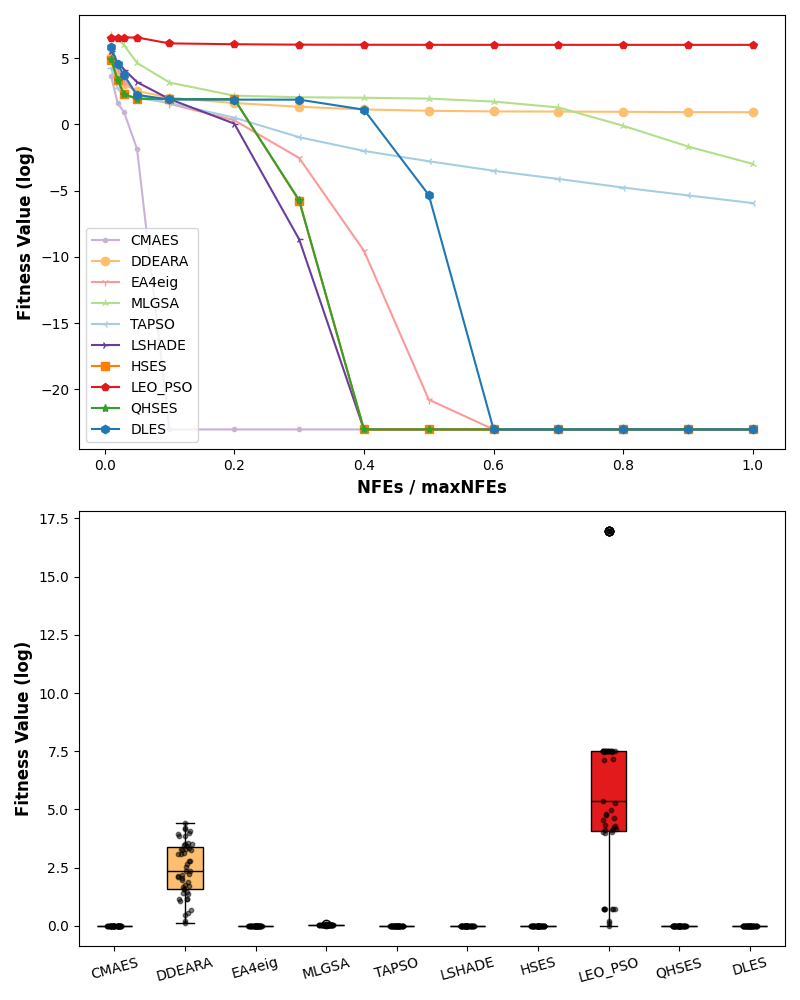
\includegraphics[width=\textwidth]{./save/D_10_F_4.png}
	\end{minipage}
	\caption{\textcolor{blue}{F1 to F3 in $D$ = 10.}}
	\label{b-p-start}
\end{figure}

% 第二组图像
\begin{figure}[H]
	\centering
	\begin{minipage}[b]{0.3\textwidth}
		\centering
		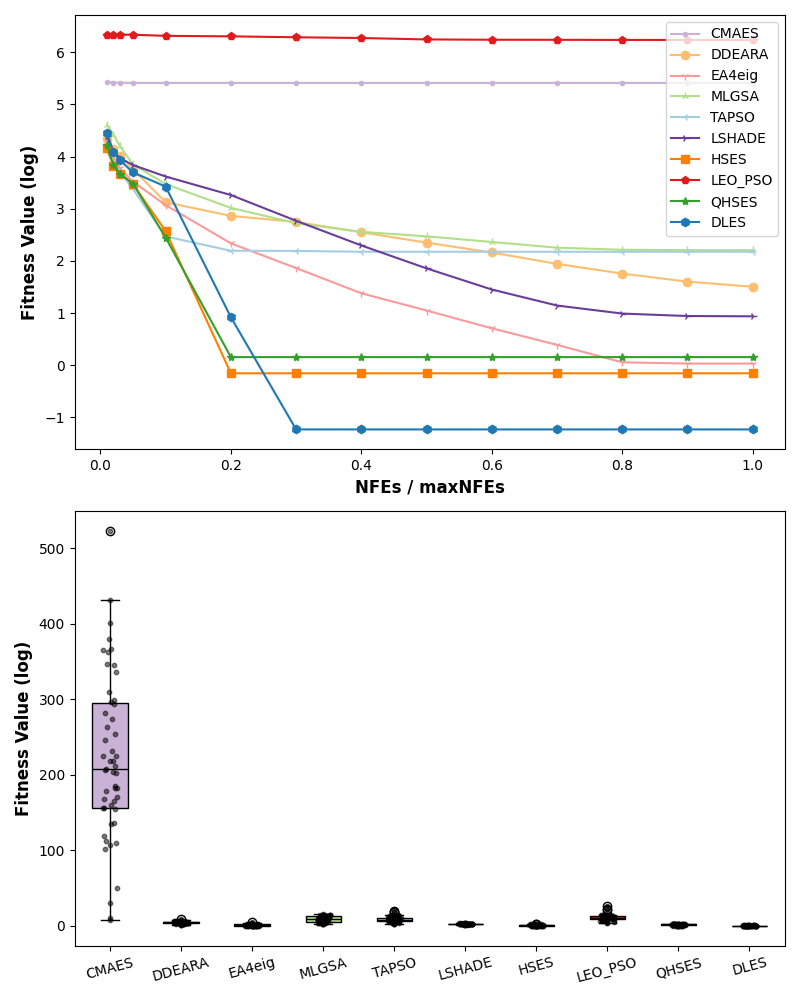
\includegraphics[width=\textwidth]{./save/D_10_F_5.png}
	\end{minipage}\hfill
	\begin{minipage}[b]{0.3\textwidth}
		\centering
		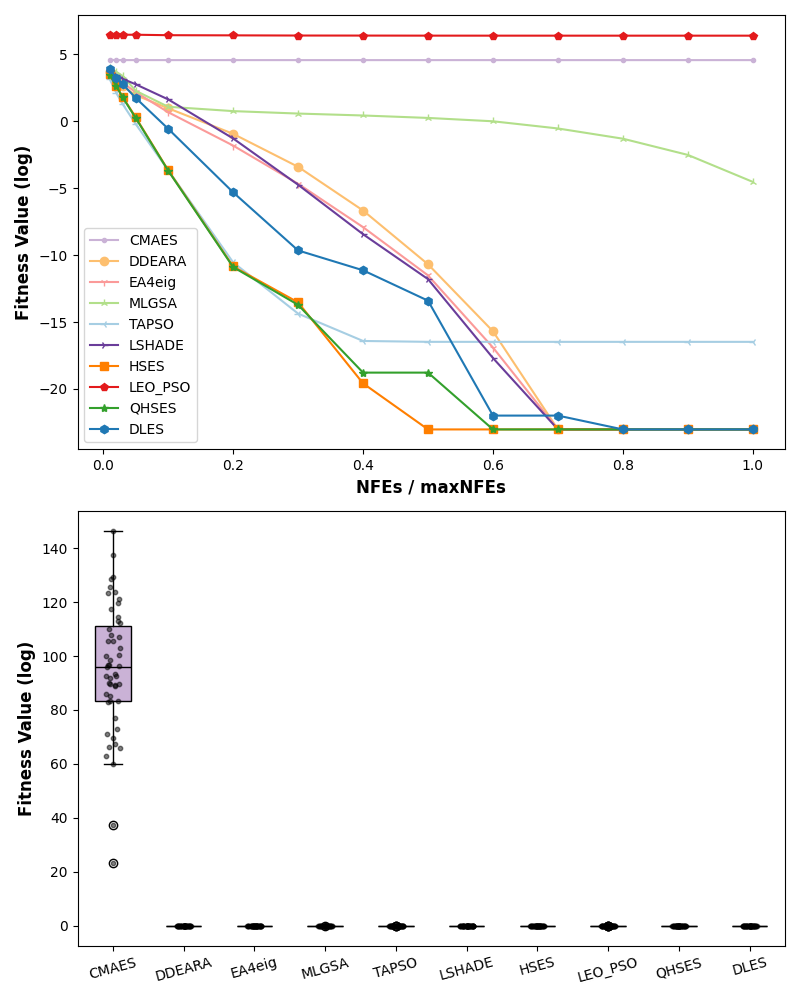
\includegraphics[width=\textwidth]{./save/D_10_F_6.png}
	\end{minipage}\hfill
	\begin{minipage}[b]{0.3\textwidth}
		\centering
		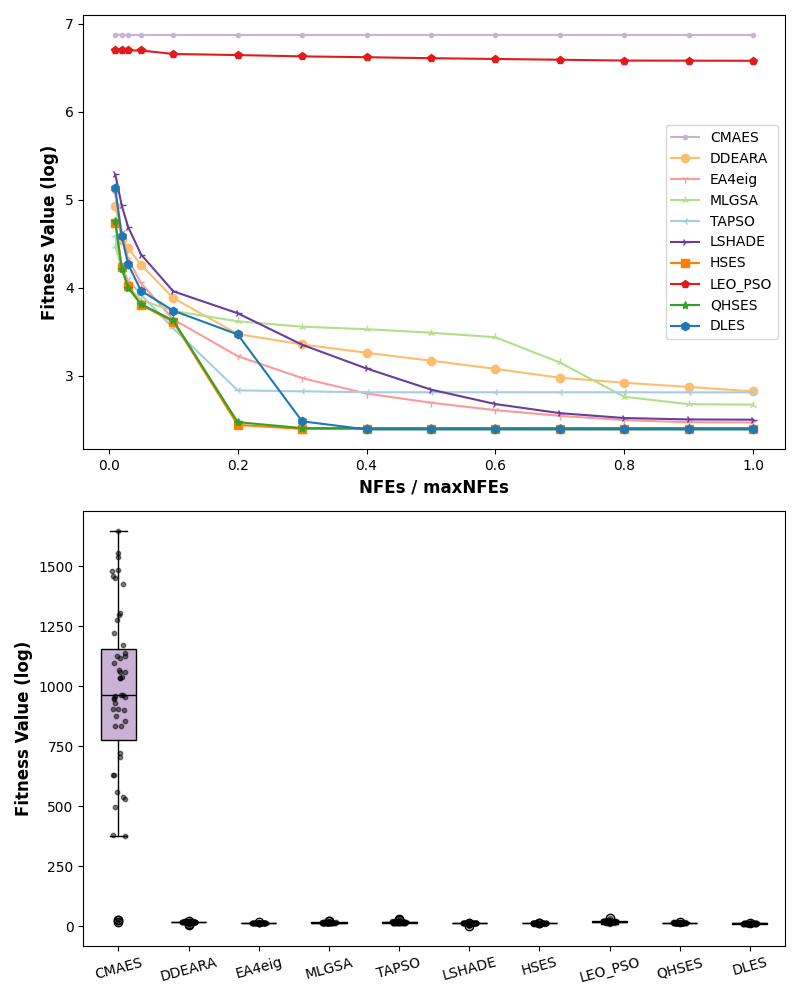
\includegraphics[width=\textwidth]{./save/D_10_F_7.png}
	\end{minipage}
	\caption{\textcolor{blue}{F4 to F6 in $D$ = 10.}}
\end{figure}

% 第三组图像
\begin{figure}[H]
	\centering
	\begin{minipage}[b]{0.3\textwidth}
		\centering
		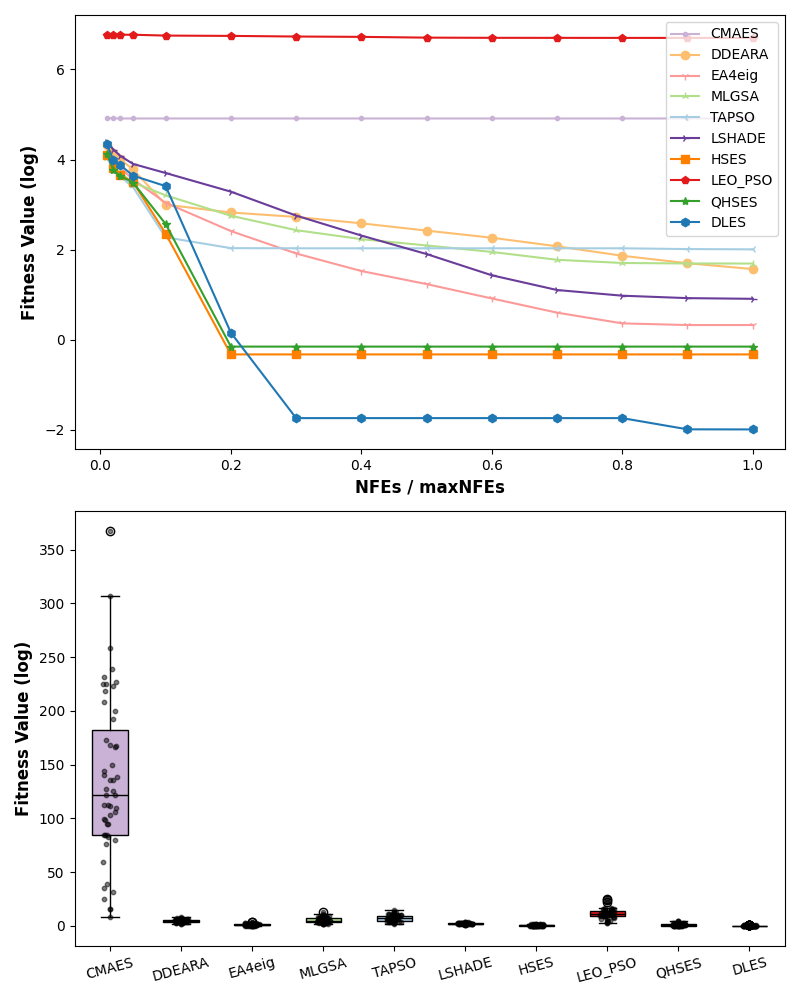
\includegraphics[width=\textwidth]{./save/D_10_F_8.png}
	\end{minipage}\hfill
	\begin{minipage}[b]{0.3\textwidth}
		\centering
		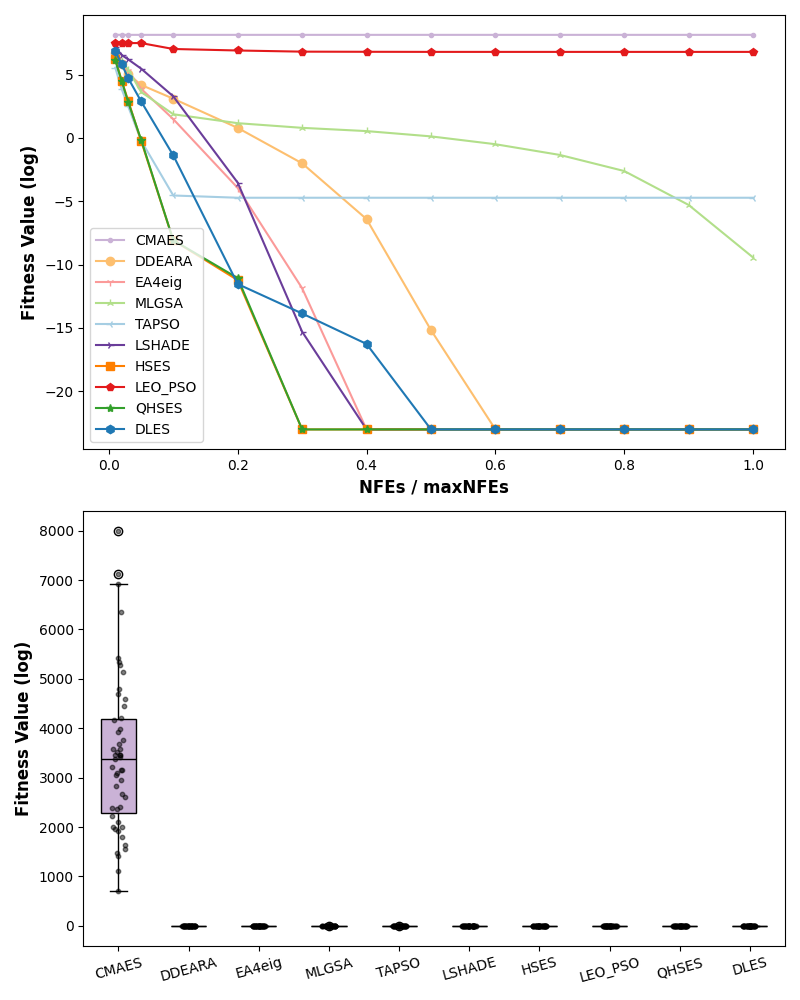
\includegraphics[width=\textwidth]{./save/D_10_F_9.png}
	\end{minipage}\hfill
	\begin{minipage}[b]{0.3\textwidth}
		\centering
		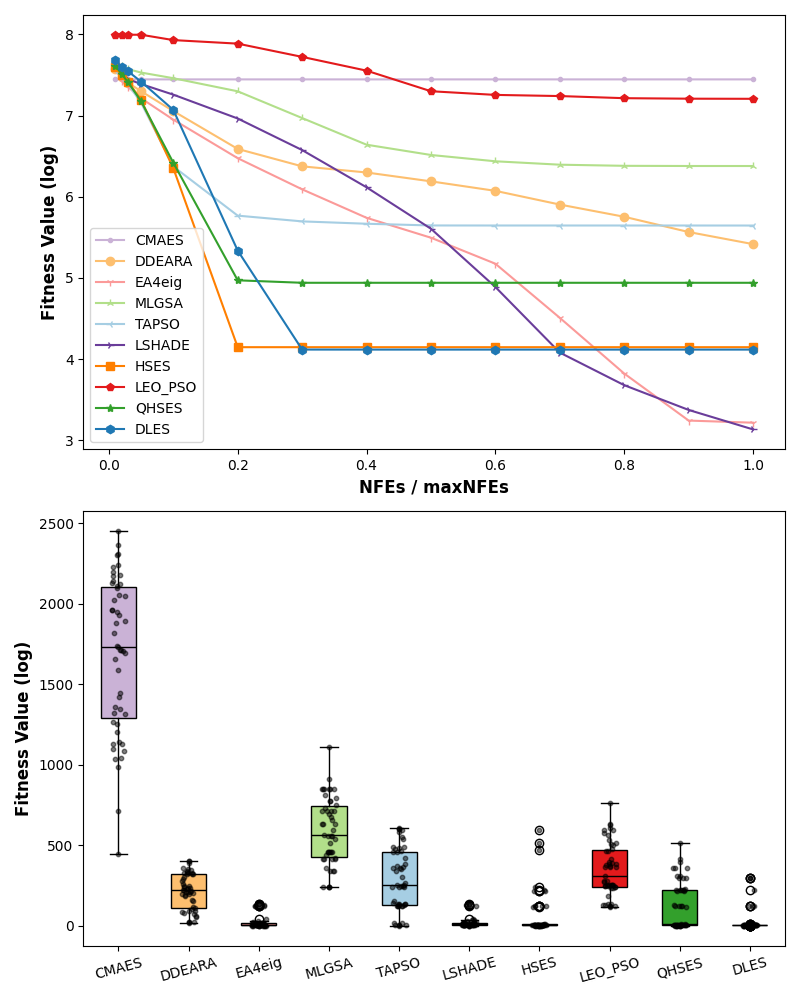
\includegraphics[width=\textwidth]{./save/D_10_F_10.png}
	\end{minipage}
	\caption{\textcolor{blue}{F7 to F9 in $D$ = 10.}}
\end{figure}

% 第四组图像
\begin{figure}[H]
	\centering
	\begin{minipage}[b]{0.3\textwidth}
		\centering
		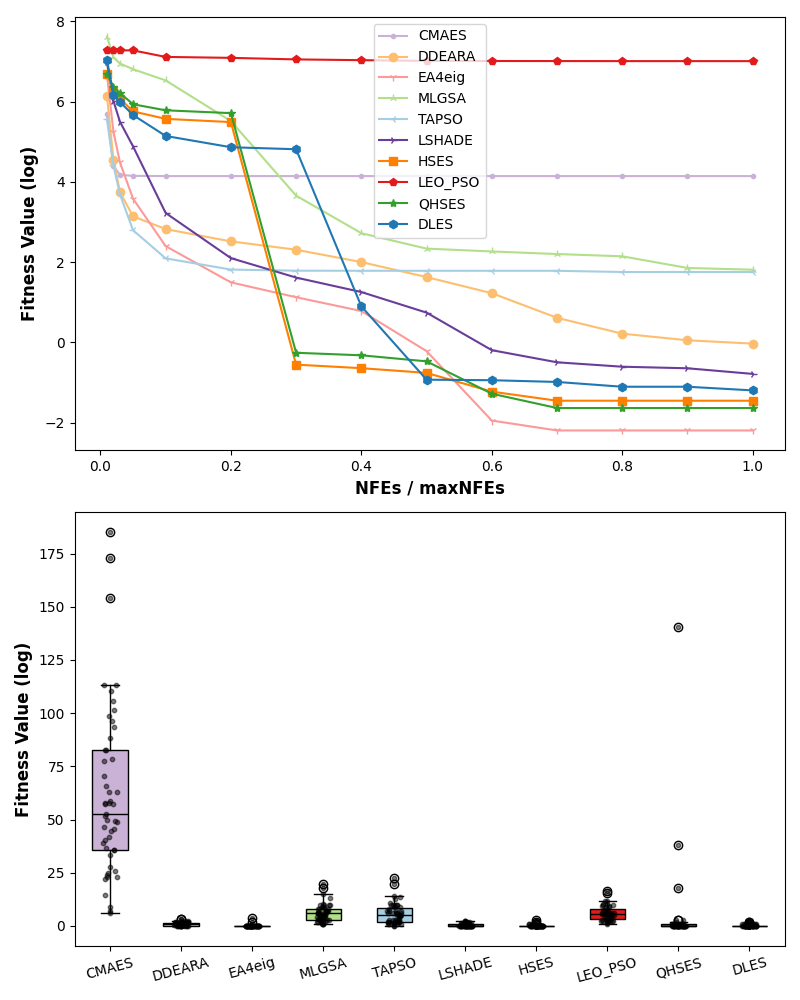
\includegraphics[width=\textwidth]{./save/D_10_F_11.png}
	\end{minipage}\hfill
	\begin{minipage}[b]{0.3\textwidth}
		\centering
		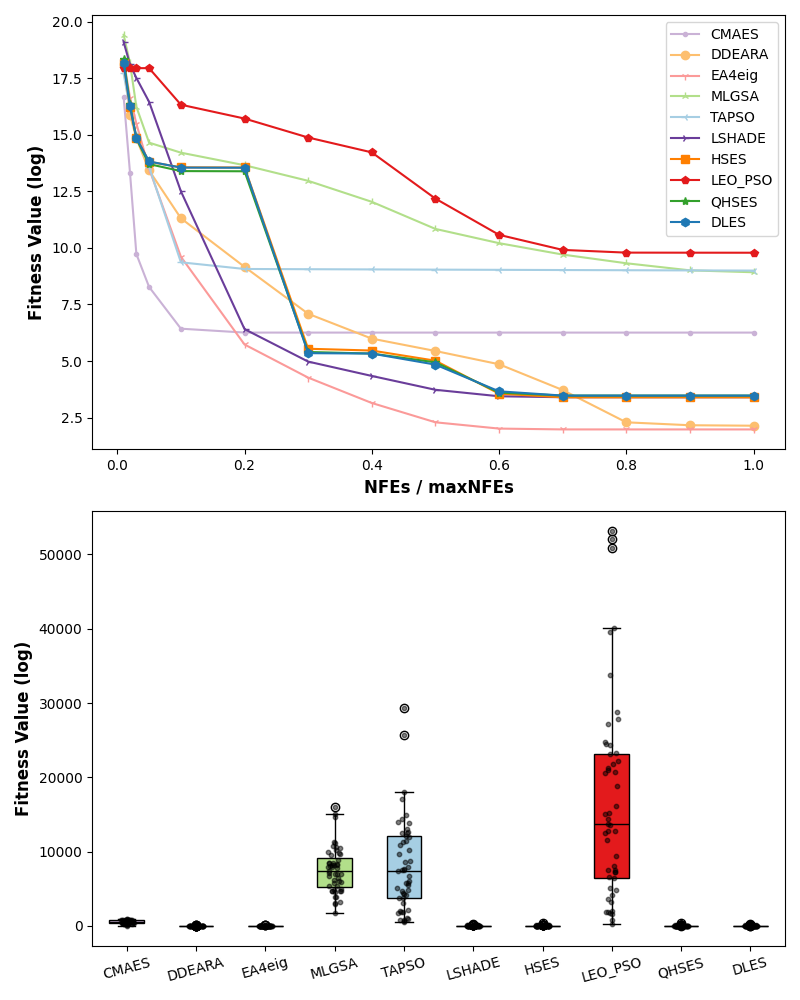
\includegraphics[width=\textwidth]{./save/D_10_F_12.png}
	\end{minipage}\hfill
	\begin{minipage}[b]{0.3\textwidth}
		\centering
		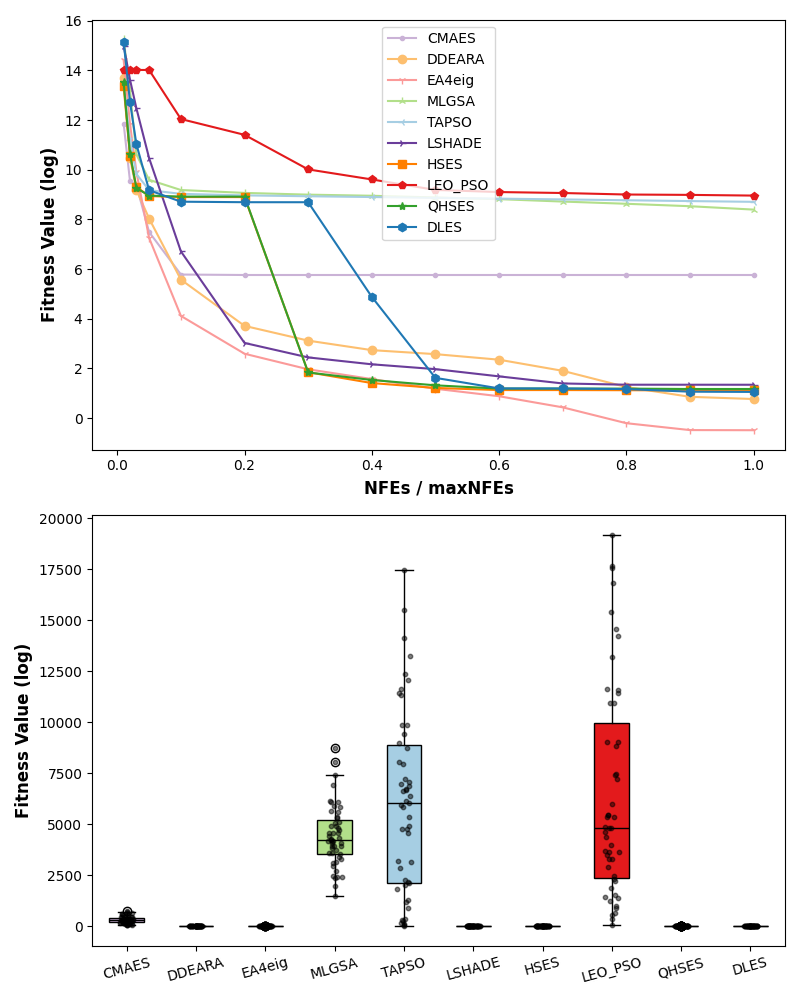
\includegraphics[width=\textwidth]{./save/D_10_F_13.png}
	\end{minipage}
	\caption{\textcolor{blue}{F10 to F12 in $D$ = 10.}}
\end{figure}

% 第五组图像
\begin{figure}[H]
	\centering
	\begin{minipage}[b]{0.3\textwidth}
		\centering
		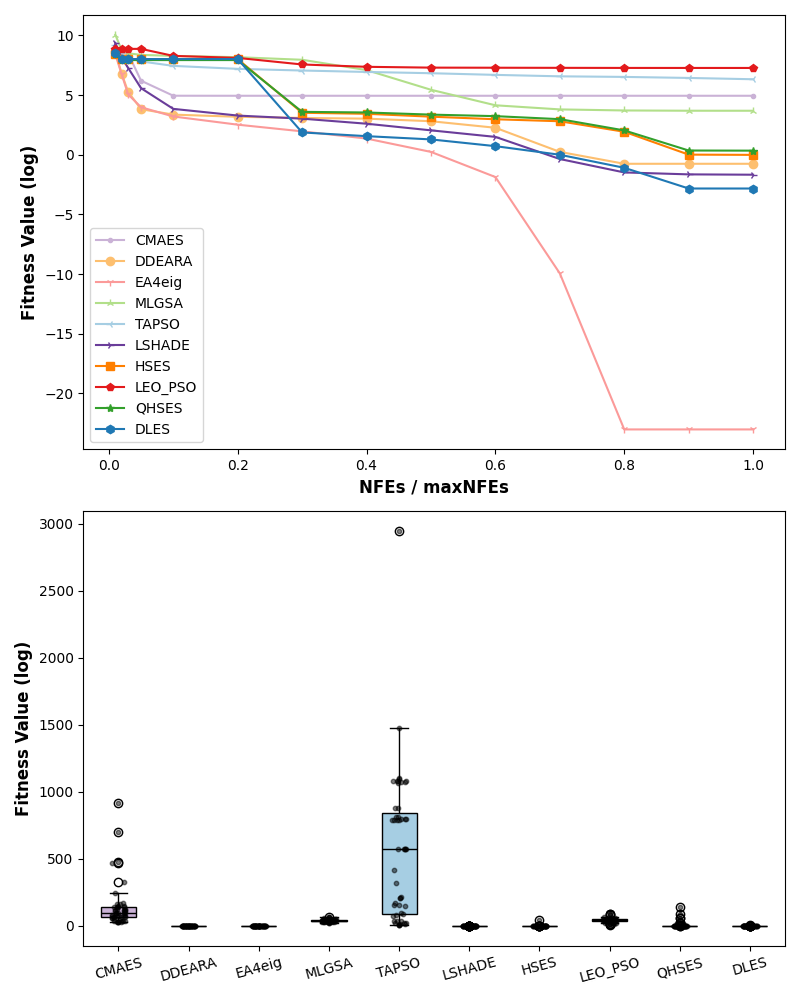
\includegraphics[width=\textwidth]{./save/D_10_F_14.png}
	\end{minipage}\hfill
	\begin{minipage}[b]{0.3\textwidth}
		\centering
		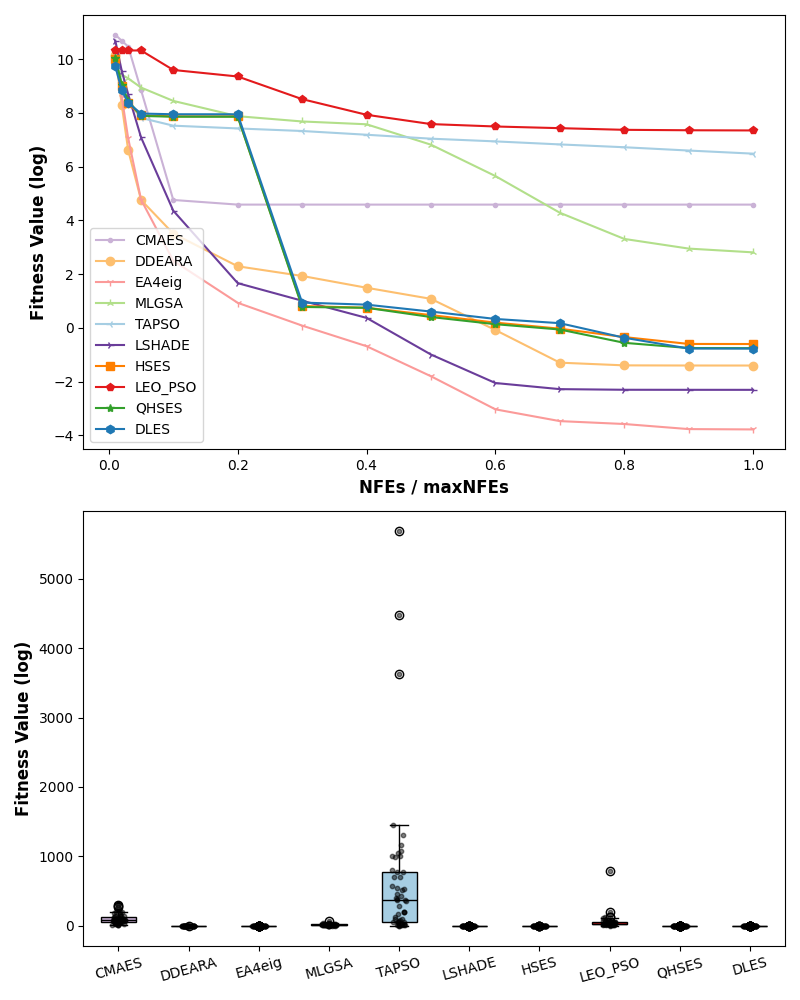
\includegraphics[width=\textwidth]{./save/D_10_F_15.png}
	\end{minipage}\hfill
	\begin{minipage}[b]{0.3\textwidth}
		\centering
		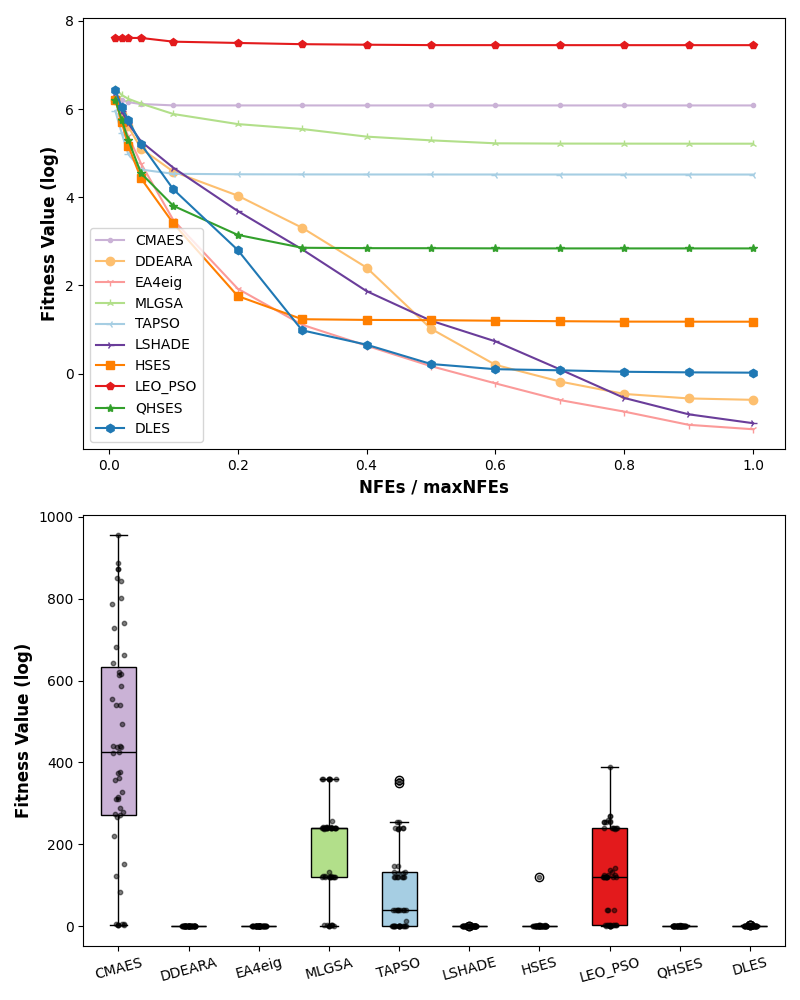
\includegraphics[width=\textwidth]{./save/D_10_F_16.png}
	\end{minipage}
	\caption{\textcolor{blue}{F13 to F15 in $D$ = 10.}}
\end{figure}

% 第六组图像
\begin{figure}[H]
	\centering
	\begin{minipage}[b]{0.3\textwidth}
		\centering
		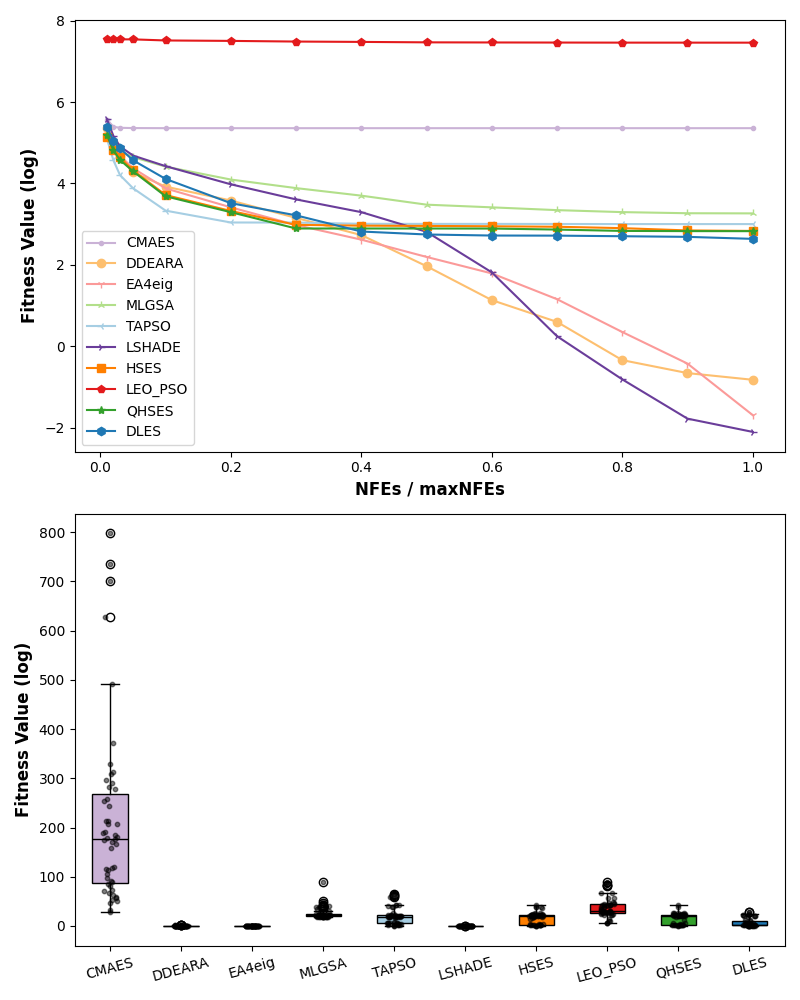
\includegraphics[width=\textwidth]{./save/D_10_F_17.png}
	\end{minipage}\hfill
	\begin{minipage}[b]{0.3\textwidth}
		\centering
		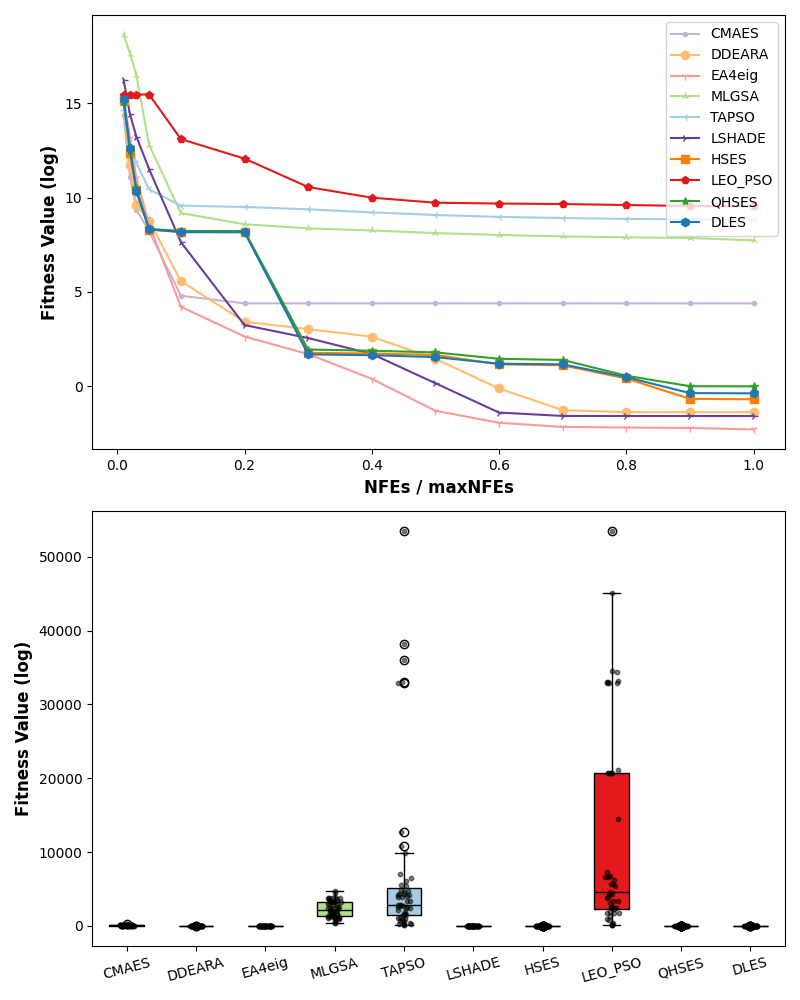
\includegraphics[width=\textwidth]{./save/D_10_F_18.png}
	\end{minipage}\hfill
	\begin{minipage}[b]{0.3\textwidth}
		\centering
		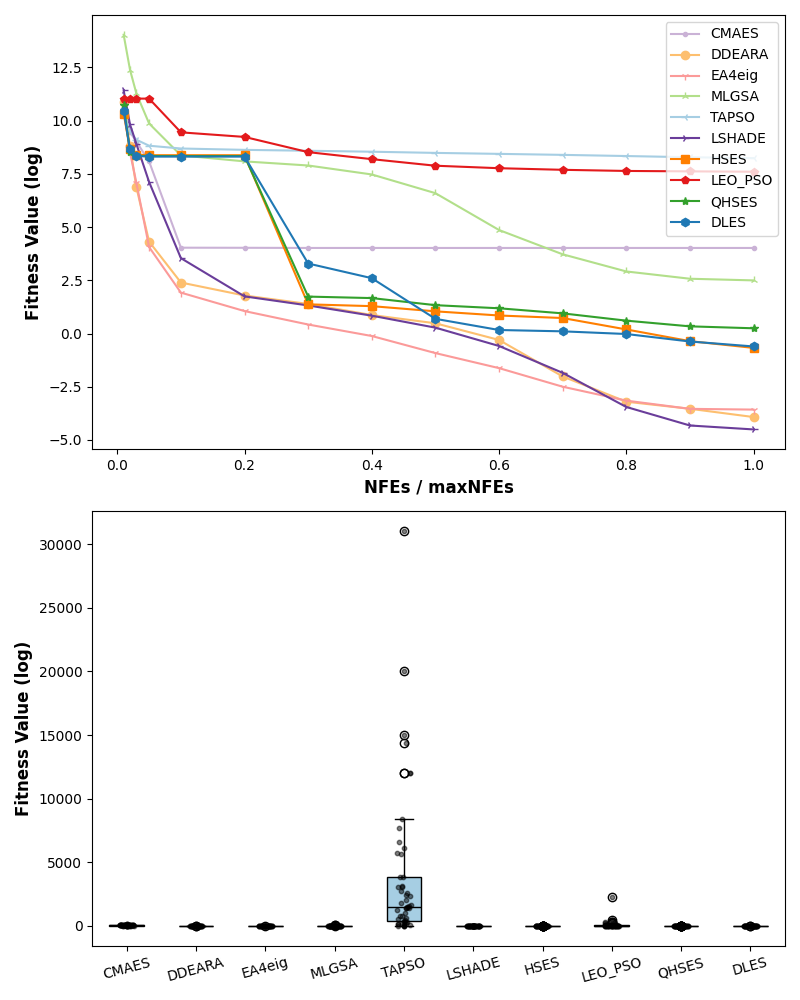
\includegraphics[width=\textwidth]{./save/D_10_F_19.png}
	\end{minipage}
	\caption{\textcolor{blue}{F16 to F18 in $D$ = 10.}}
\end{figure}

% 第七组图像
\begin{figure}[H]
	\centering
	\begin{minipage}[b]{0.3\textwidth}
		\centering
		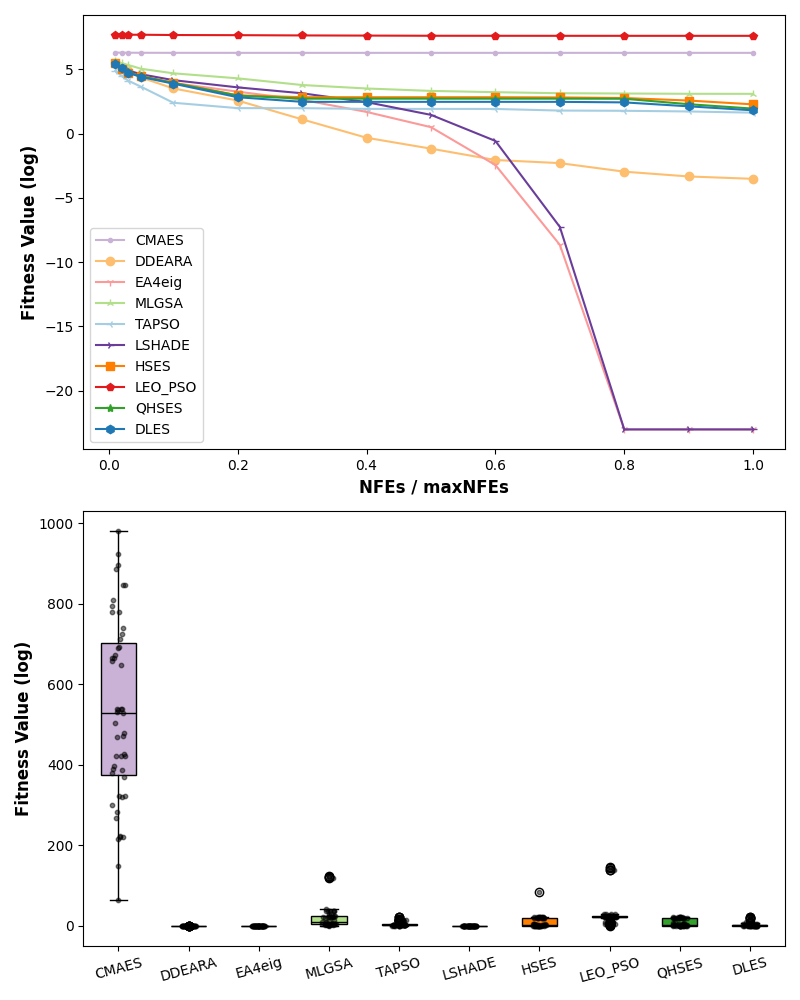
\includegraphics[width=\textwidth]{./save/D_10_F_20.png}
	\end{minipage}\hfill
	\begin{minipage}[b]{0.3\textwidth}
		\centering
		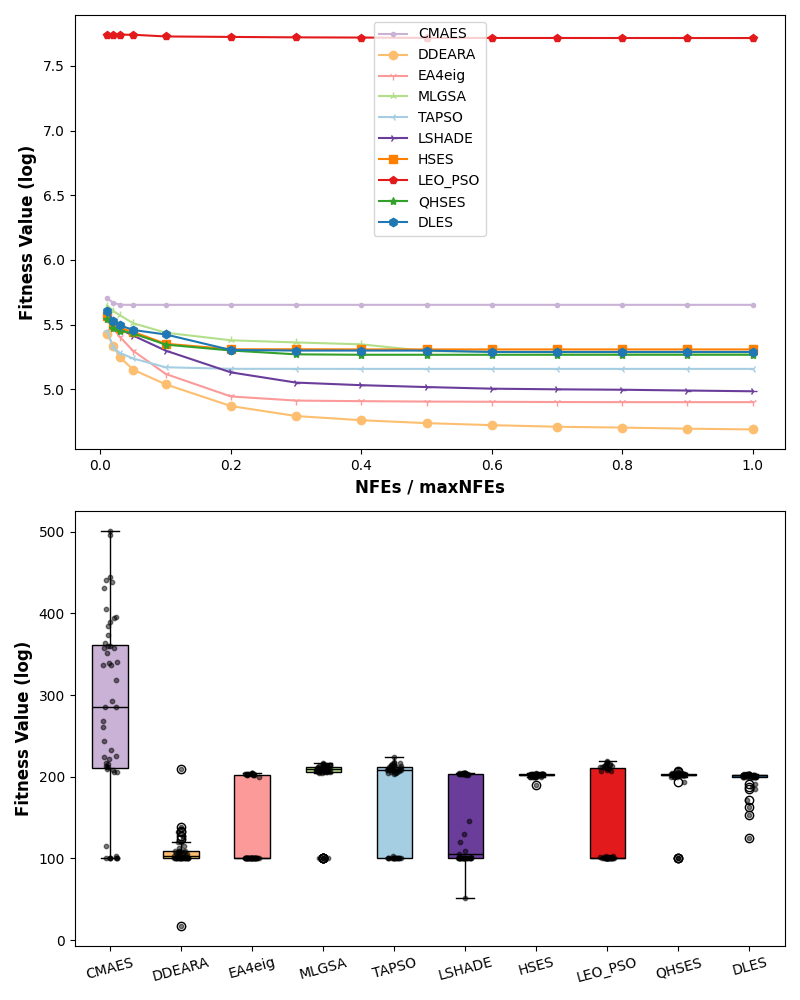
\includegraphics[width=\textwidth]{./save/D_10_F_21.png}
	\end{minipage}\hfill
	\begin{minipage}[b]{0.3\textwidth}
		\centering
		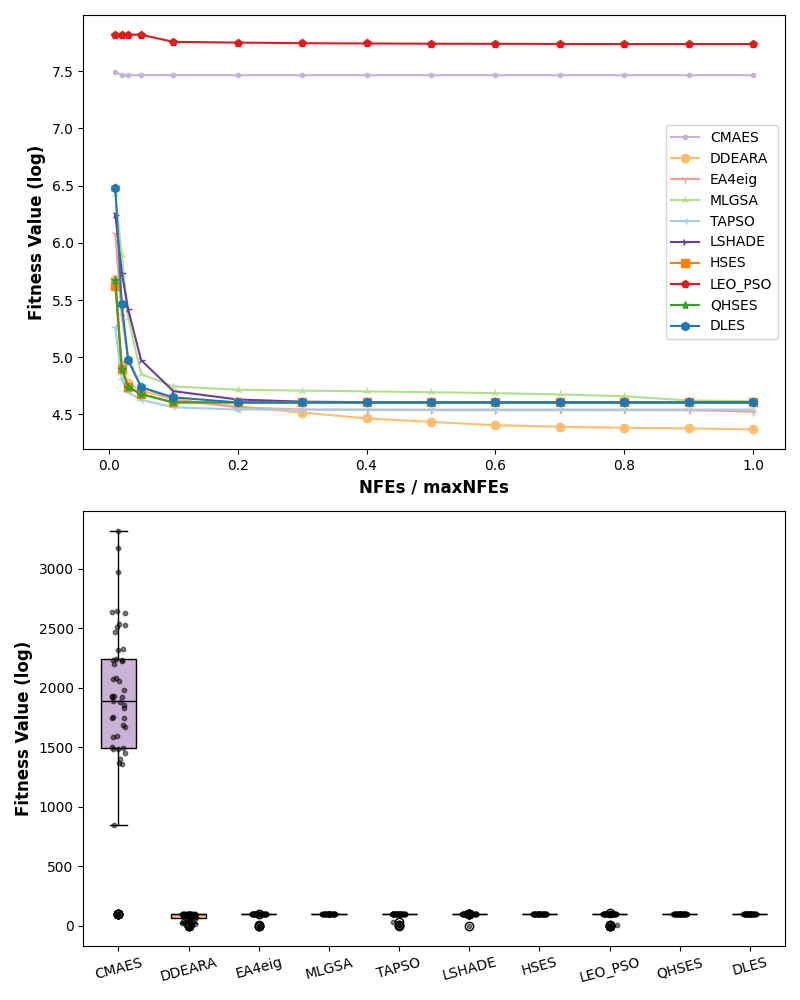
\includegraphics[width=\textwidth]{./save/D_10_F_22.png}
	\end{minipage}
	\caption{\textcolor{blue}{F19 to F21 in $D$ = 10.}}
\end{figure}

% 第八组图像
\begin{figure}[H]
	\centering
	\begin{minipage}[b]{0.3\textwidth}
		\centering
		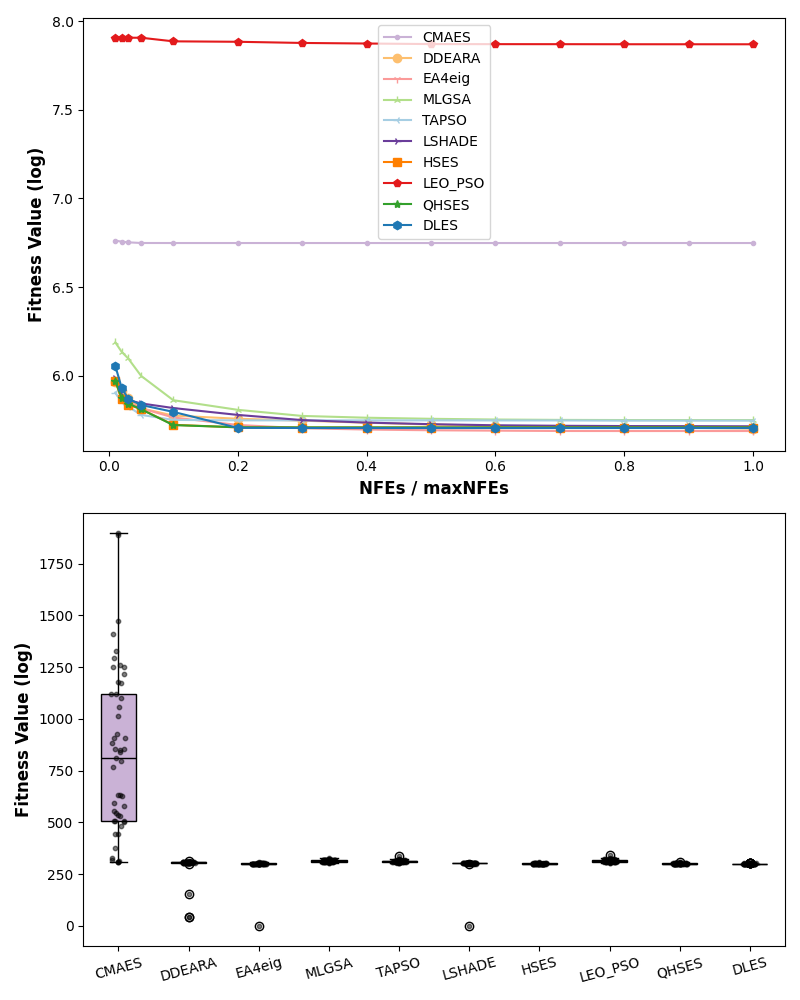
\includegraphics[width=\textwidth]{./save/D_10_F_23.png}
	\end{minipage}\hfill
	\begin{minipage}[b]{0.3\textwidth}
		\centering
		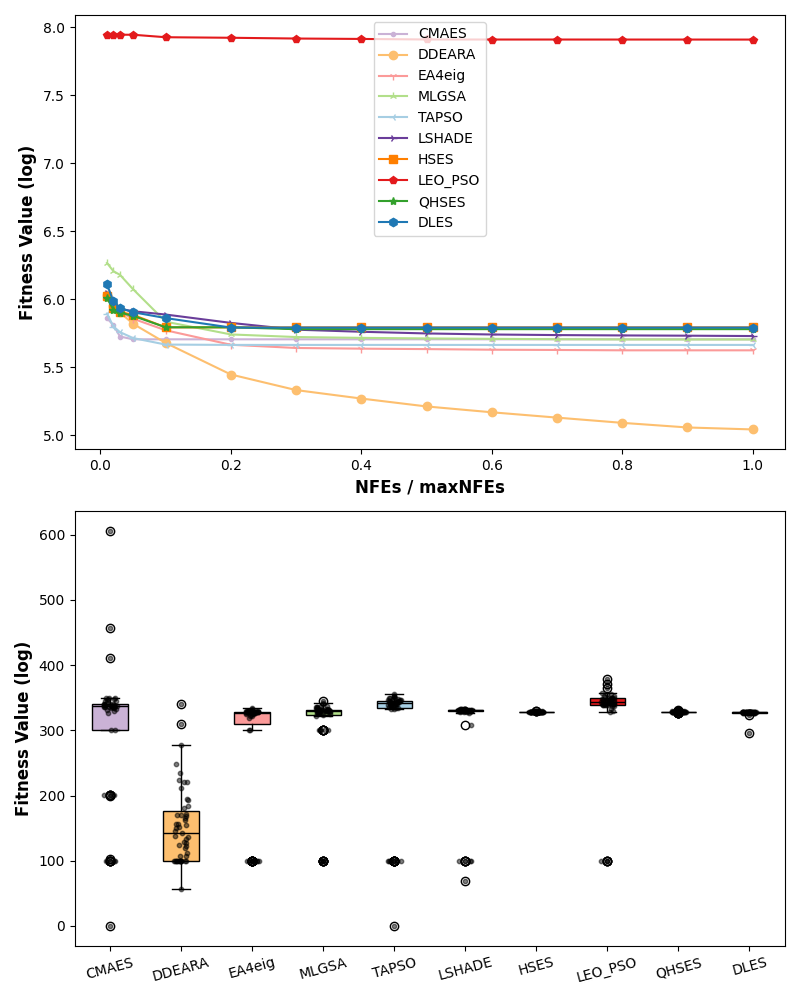
\includegraphics[width=\textwidth]{./save/D_10_F_24.png}
	\end{minipage}\hfill
	\begin{minipage}[b]{0.3\textwidth}
		\centering
		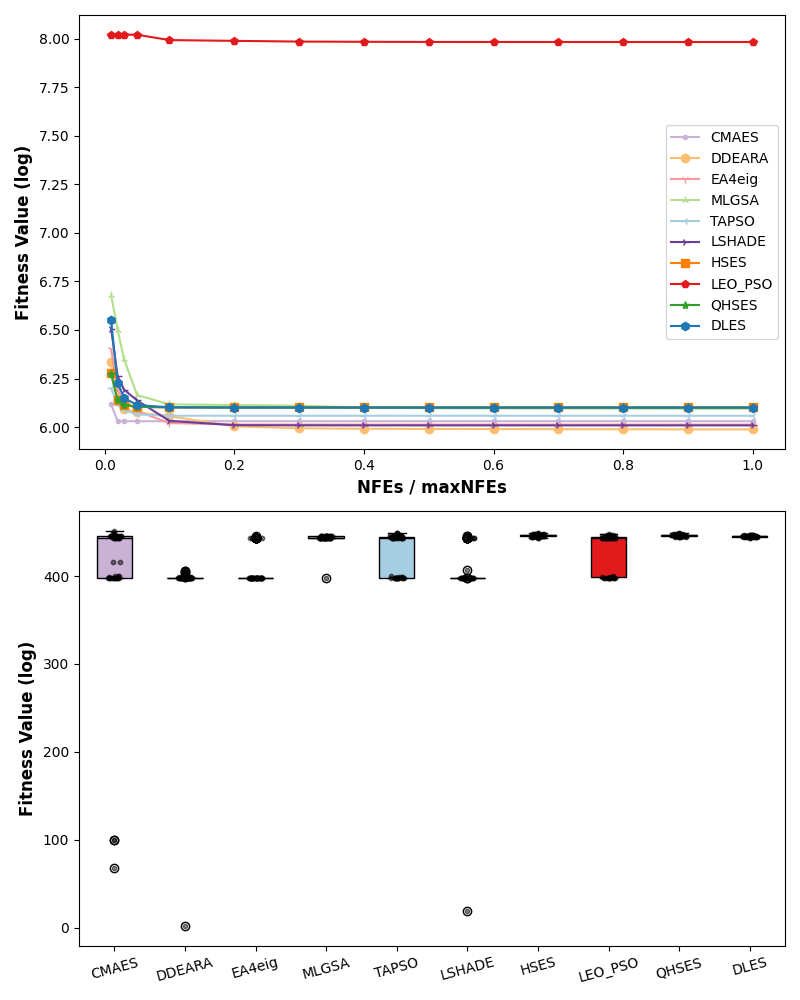
\includegraphics[width=\textwidth]{./save/D_10_F_25.png}
	\end{minipage}
	\caption{\textcolor{blue}{F22 to F24 in $D$ = 10.}}
\end{figure}

% 第九组图像
\begin{figure}[H]
	\centering
	\begin{minipage}[b]{0.3\textwidth}
		\centering
		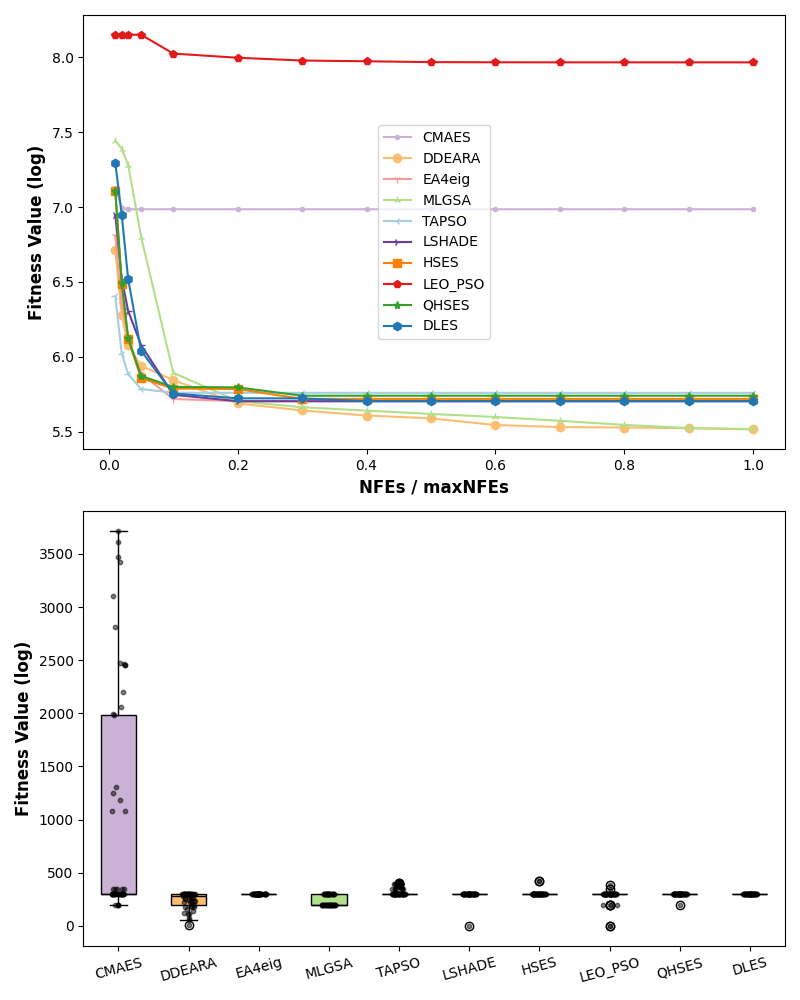
\includegraphics[width=\textwidth]{./save/D_10_F_26.png}
	\end{minipage}\hfill
	\begin{minipage}[b]{0.3\textwidth}
		\centering
		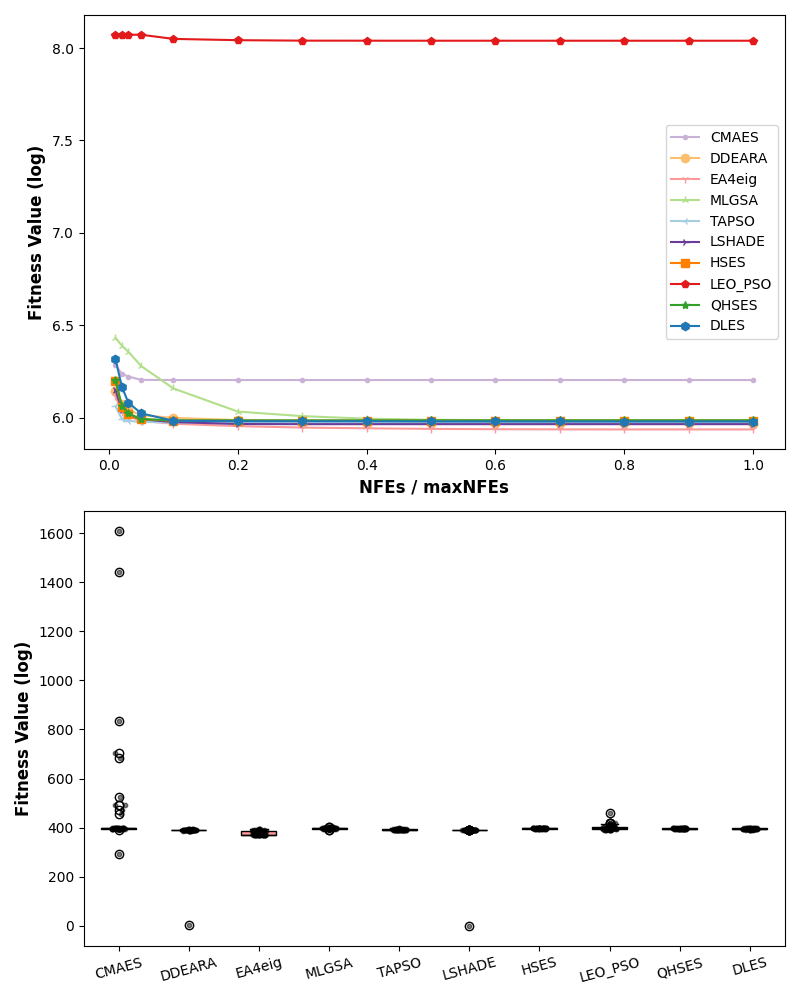
\includegraphics[width=\textwidth]{./save/D_10_F_27.png}
	\end{minipage}\hfill
	\begin{minipage}[b]{0.3\textwidth}
		\centering
		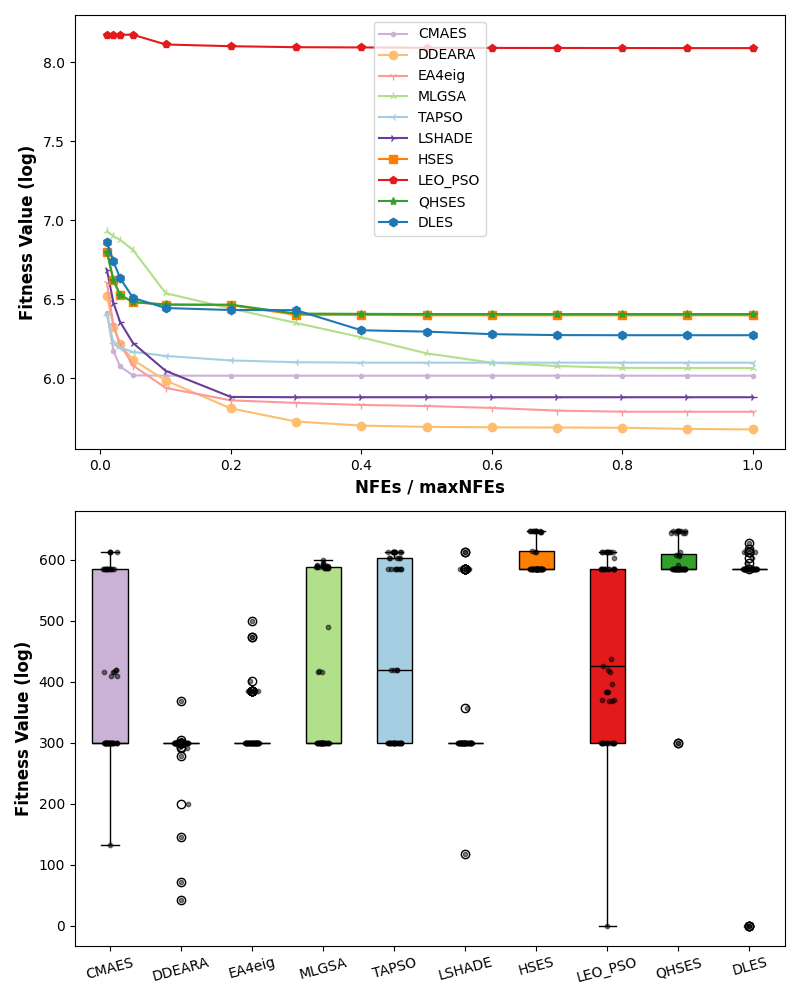
\includegraphics[width=\textwidth]{./save/D_10_F_28.png}
	\end{minipage}
	\caption{\textcolor{blue}{F25 to F27 in $D$ = 10.}}
\end{figure}

% 第十组图像
\begin{figure}[H]
	\centering
	\begin{minipage}[b]{0.3\textwidth}
		\centering
		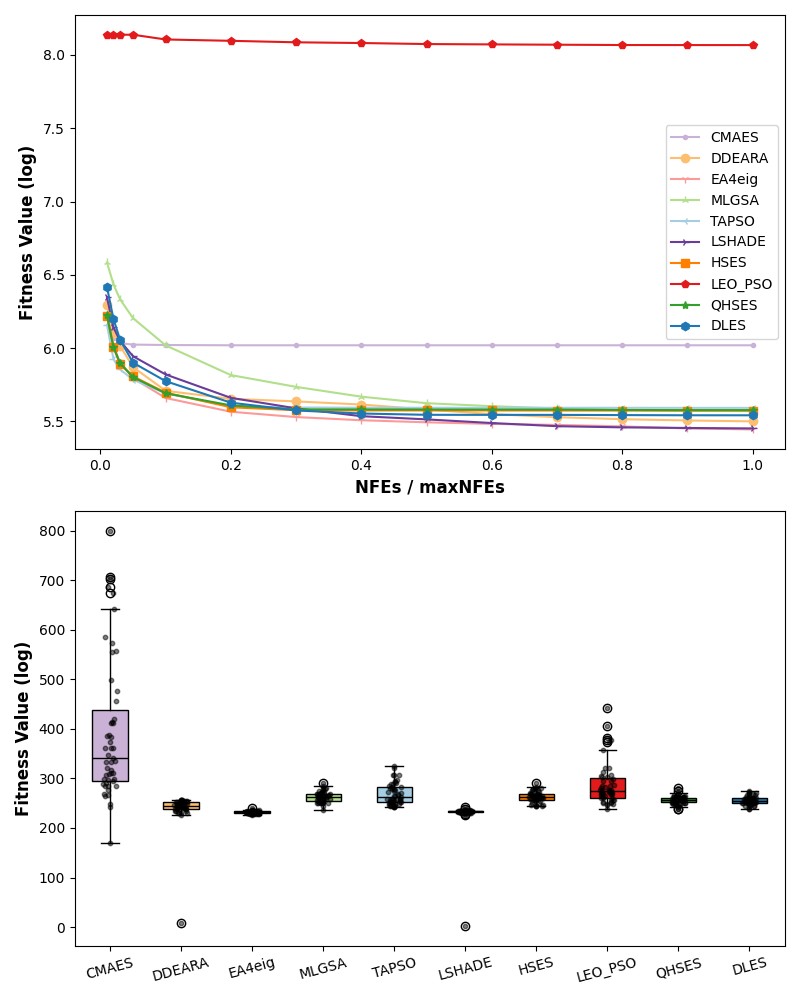
\includegraphics[width=\textwidth]{./save/D_10_F_29.png}
	\end{minipage}\hfill
	\begin{minipage}[b]{0.3\textwidth}
		\centering
		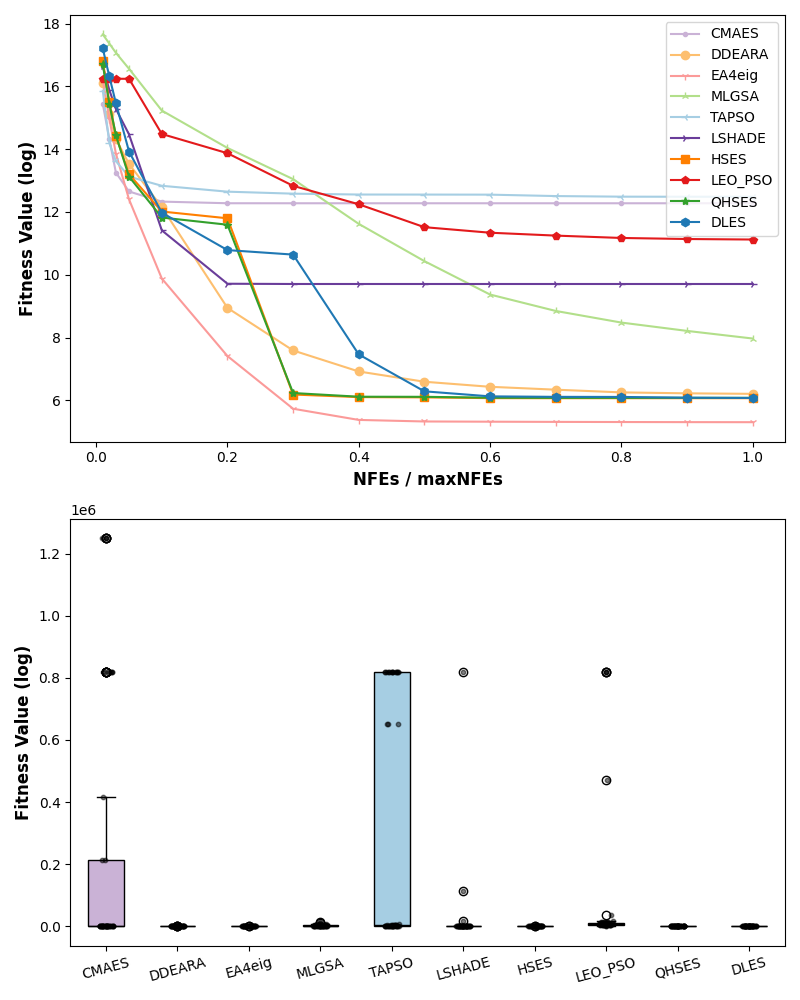
\includegraphics[width=\textwidth]{./save/D_10_F_30.png}
	\end{minipage}\hfill
	\begin{minipage}[b]{0.3\textwidth}
		\centering
		\phantom{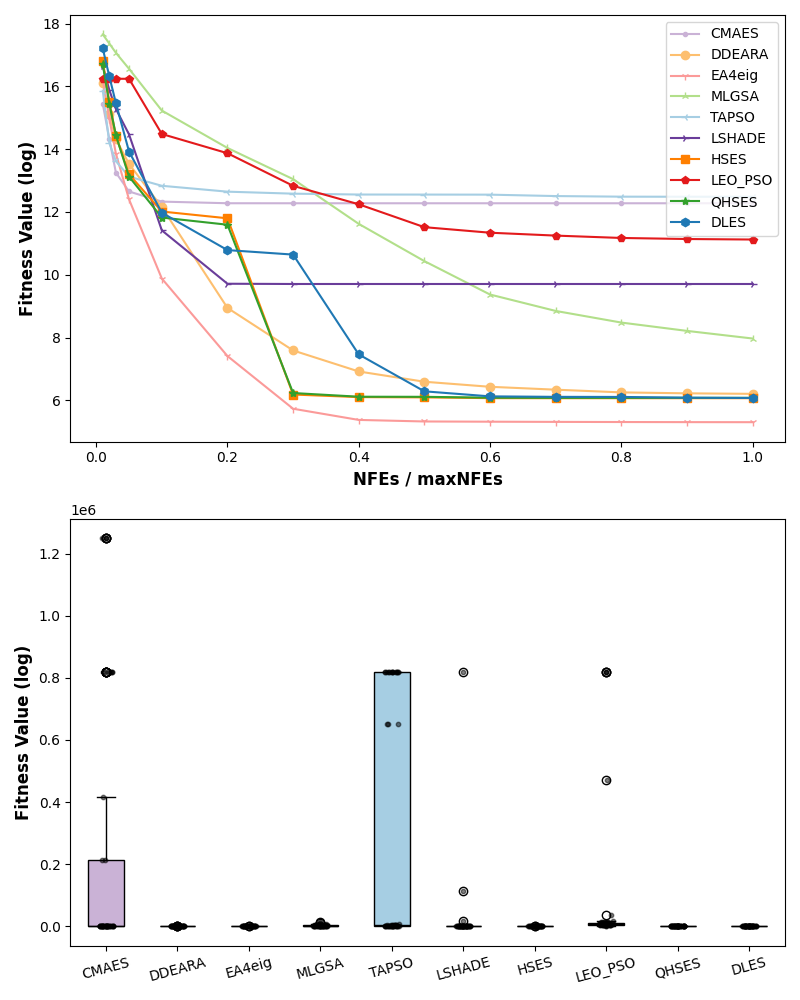
\includegraphics[width=\textwidth]{./save/D_10_F_30.png}}
	\end{minipage}
	\caption{\textcolor{blue}{F28 and F29 in $D$ = 10.}}
\end{figure}

% 第一组图像
\begin{figure}[H]
	\centering
	\begin{minipage}[b]{0.3\textwidth}
		\centering
		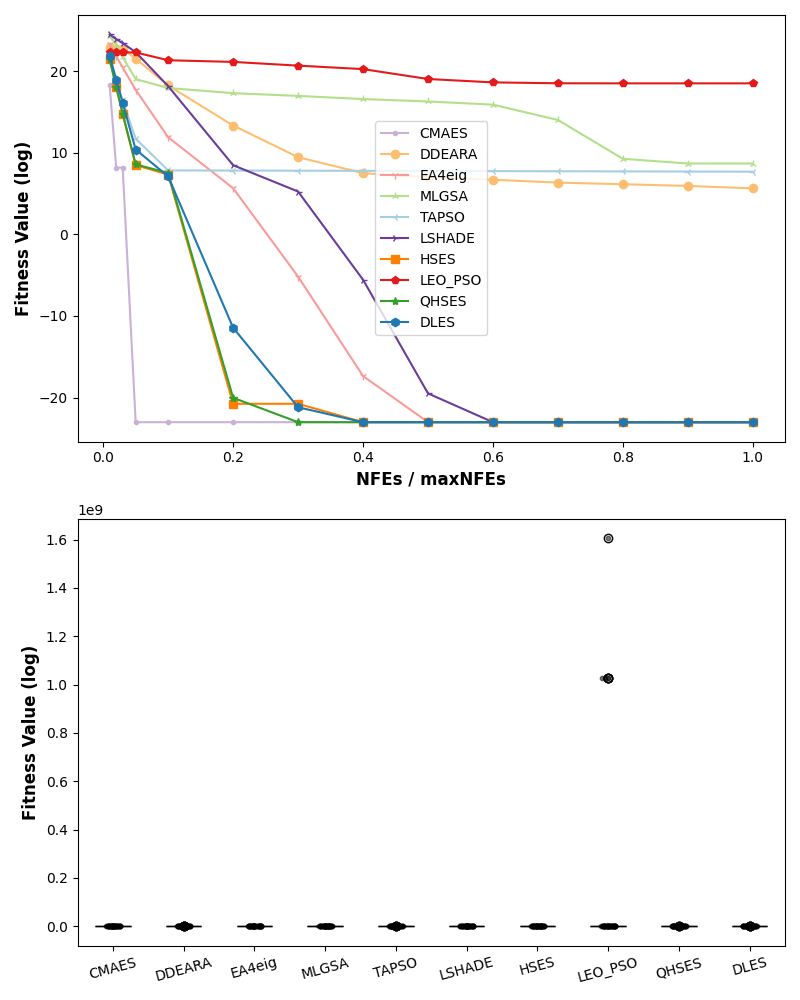
\includegraphics[width=\textwidth]{./save/D_30_F_1.png}
	\end{minipage}\hfill
	\begin{minipage}[b]{0.3\textwidth}
		\centering
		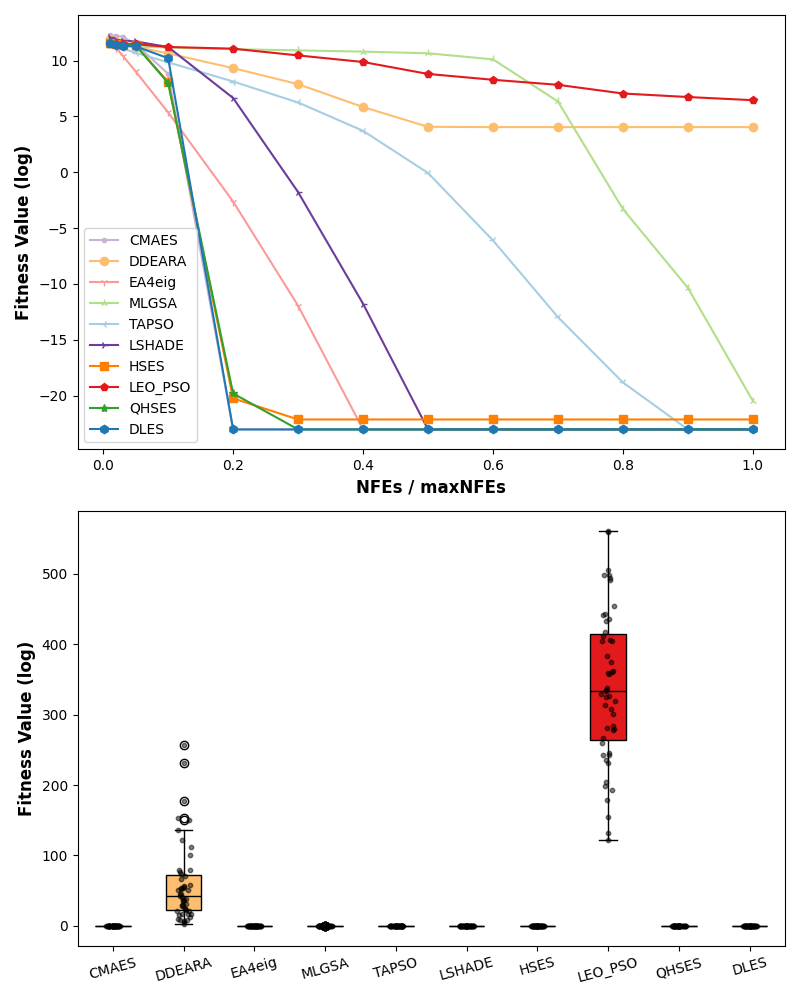
\includegraphics[width=\textwidth]{./save/D_30_F_3.png}
	\end{minipage}\hfill
	\begin{minipage}[b]{0.3\textwidth}
		\centering
		\includegraphics[width=\textwidth]{./save/D_30_F_4.png}
	\end{minipage}
	\caption{\textcolor{blue}{F1 to F3 in $D$ = 30.}}
\end{figure}

% 第二组图像
\begin{figure}[H]
	\centering
	\begin{minipage}[b]{0.3\textwidth}
		\centering
		\includegraphics[width=\textwidth]{./save/D_30_F_5.png}
	\end{minipage}\hfill
	\begin{minipage}[b]{0.3\textwidth}
		\centering
		\includegraphics[width=\textwidth]{./save/D_30_F_6.png}
	\end{minipage}\hfill
	\begin{minipage}[b]{0.3\textwidth}
		\centering
		\includegraphics[width=\textwidth]{./save/D_30_F_7.png}
	\end{minipage}
	\caption{\textcolor{blue}{F4 to F6 in $D$ = 30.}}
\end{figure}

% 第三组图像
\begin{figure}[H]
	\centering
	\begin{minipage}[b]{0.3\textwidth}
		\centering
		\includegraphics[width=\textwidth]{./save/D_30_F_8.png}
	\end{minipage}\hfill
	\begin{minipage}[b]{0.3\textwidth}
		\centering
		\includegraphics[width=\textwidth]{./save/D_30_F_9.png}
	\end{minipage}\hfill
	\begin{minipage}[b]{0.3\textwidth}
		\centering
		\includegraphics[width=\textwidth]{./save/D_30_F_10.png}
	\end{minipage}
	\caption{\textcolor{blue}{F7 to F9 in $D$ = 30.}}
\end{figure}

% 第四组图像
\begin{figure}[H]
	\centering
	\begin{minipage}[b]{0.3\textwidth}
		\centering
		\includegraphics[width=\textwidth]{./save/D_30_F_11.png}
	\end{minipage}\hfill
	\begin{minipage}[b]{0.3\textwidth}
		\centering
		\includegraphics[width=\textwidth]{./save/D_30_F_12.png}
	\end{minipage}\hfill
	\begin{minipage}[b]{0.3\textwidth}
		\centering
		\includegraphics[width=\textwidth]{./save/D_30_F_13.png}
	\end{minipage}
	\caption{\textcolor{blue}{F11 to F13 in $D$ = 30.}}
\end{figure}

% 第五组图像
\begin{figure}[H]
	\centering
	\begin{minipage}[b]{0.3\textwidth}
		\centering
		\includegraphics[width=\textwidth]{./save/D_30_F_14.png}
	\end{minipage}\hfill
	\begin{minipage}[b]{0.3\textwidth}
		\centering
		\includegraphics[width=\textwidth]{./save/D_30_F_15.png}
	\end{minipage}\hfill
	\begin{minipage}[b]{0.3\textwidth}
		\centering
		\includegraphics[width=\textwidth]{./save/D_30_F_16.png}
	\end{minipage}
	\caption{\textcolor{blue}{F14 to F16 in $D$ = 30.}}
\end{figure}

% 第六组图像
\begin{figure}[H]
	\centering
	\begin{minipage}[b]{0.3\textwidth}
		\centering
		\includegraphics[width=\textwidth]{./save/D_30_F_17.png}
	\end{minipage}\hfill
	\begin{minipage}[b]{0.3\textwidth}
		\centering
		\includegraphics[width=\textwidth]{./save/D_30_F_18.png}
	\end{minipage}\hfill
	\begin{minipage}[b]{0.3\textwidth}
		\centering
		\includegraphics[width=\textwidth]{./save/D_30_F_19.png}
	\end{minipage}
	\caption{\textcolor{blue}{F17 to F19 in $D$ = 30.}}
\end{figure}

% 第七组图像
\begin{figure}[H]
	\centering
	\begin{minipage}[b]{0.3\textwidth}
		\centering
		\includegraphics[width=\textwidth]{./save/D_30_F_20.png}
	\end{minipage}\hfill
	\begin{minipage}[b]{0.3\textwidth}
		\centering
		\includegraphics[width=\textwidth]{./save/D_30_F_21.png}
	\end{minipage}\hfill
	\begin{minipage}[b]{0.3\textwidth}
		\centering
		\includegraphics[width=\textwidth]{./save/D_30_F_22.png}
	\end{minipage}
	\caption{\textcolor{blue}{F20 to F22 in $D$ = 30.}}
\end{figure}

% 第八组图像
\begin{figure}[H]
	\centering
	\begin{minipage}[b]{0.3\textwidth}
		\centering
		\includegraphics[width=\textwidth]{./save/D_30_F_23.png}
	\end{minipage}\hfill
	\begin{minipage}[b]{0.3\textwidth}
		\centering
		\includegraphics[width=\textwidth]{./save/D_30_F_24.png}
	\end{minipage}\hfill
	\begin{minipage}[b]{0.3\textwidth}
		\centering
		\includegraphics[width=\textwidth]{./save/D_30_F_25.png}
	\end{minipage}
	\caption{\textcolor{blue}{F23 to F25 in $D$ = 30.}}
\end{figure}

% 第九组图像
\begin{figure}[H]
	\centering
	\begin{minipage}[b]{0.3\textwidth}
		\centering
		\includegraphics[width=\textwidth]{./save/D_30_F_26.png}
	\end{minipage}\hfill
	\begin{minipage}[b]{0.3\textwidth}
		\centering
		\includegraphics[width=\textwidth]{./save/D_30_F_27.png}
	\end{minipage}\hfill
	\begin{minipage}[b]{0.3\textwidth}
		\centering
		\includegraphics[width=\textwidth]{./save/D_30_F_28.png}
	\end{minipage}
	\caption{\textcolor{blue}{F26 to F28 in $D$ = 30.}}
\end{figure}

% 第十组图像
\begin{figure}[H]
	\centering
	\begin{minipage}[b]{0.3\textwidth}
		\centering
		\includegraphics[width=\textwidth]{./save/D_30_F_29.png}
	\end{minipage}\hfill
	\begin{minipage}[b]{0.3\textwidth}
		\centering
		\includegraphics[width=\textwidth]{./save/D_30_F_30.png}
	\end{minipage}\hfill
	\begin{minipage}[b]{0.3\textwidth}
		\centering
		\phantom{\includegraphics[width=\textwidth]{./save/D_10_F_30.png}}
	\end{minipage}
	\caption{\textcolor{blue}{F29 and F30 in $D$ = 30.}}
\end{figure}

% 第一组图像
\begin{figure}[H]
	\centering
	\begin{minipage}[b]{0.3\textwidth}
		\centering
		\includegraphics[width=\textwidth]{./save/D_50_F_1.png}
	\end{minipage}\hfill
	\begin{minipage}[b]{0.3\textwidth}
		\centering
		\includegraphics[width=\textwidth]{./save/D_50_F_3.png}
	\end{minipage}\hfill
	\begin{minipage}[b]{0.3\textwidth}
		\centering
		\includegraphics[width=\textwidth]{./save/D_50_F_4.png}
	\end{minipage}
	\caption{\textcolor{blue}{F1 to F3 in $D$ = 50.}}
\end{figure}

% 第二组图像
\begin{figure}[H]
	\centering
	\begin{minipage}[b]{0.3\textwidth}
		\centering
		\includegraphics[width=\textwidth]{./save/D_50_F_5.png}
	\end{minipage}\hfill
	\begin{minipage}[b]{0.3\textwidth}
		\centering
		\includegraphics[width=\textwidth]{./save/D_50_F_6.png}
	\end{minipage}\hfill
	\begin{minipage}[b]{0.3\textwidth}
		\centering
		\includegraphics[width=\textwidth]{./save/D_50_F_7.png}
	\end{minipage}
	\caption{\textcolor{blue}{F4 to F6 in $D$ = 50.}}
\end{figure}

% 第三组图像
\begin{figure}[H]
	\centering
	\begin{minipage}[b]{0.3\textwidth}
		\centering
		\includegraphics[width=\textwidth]{./save/D_50_F_8.png}
	\end{minipage}\hfill
	\begin{minipage}[b]{0.3\textwidth}
		\centering
		\includegraphics[width=\textwidth]{./save/D_50_F_9.png}
	\end{minipage}\hfill
	\begin{minipage}[b]{0.3\textwidth}
		\centering
		\includegraphics[width=\textwidth]{./save/D_50_F_10.png}
	\end{minipage}
	\caption{\textcolor{blue}{F7 to F9 in $D$ = 50.}}
\end{figure}

% 第四组图像
\begin{figure}[H]
	\centering
	\begin{minipage}[b]{0.3\textwidth}
		\centering
		\includegraphics[width=\textwidth]{./save/D_50_F_11.png}
	\end{minipage}\hfill
	\begin{minipage}[b]{0.3\textwidth}
		\centering
		\includegraphics[width=\textwidth]{./save/D_50_F_12.png}
	\end{minipage}\hfill
	\begin{minipage}[b]{0.3\textwidth}
		\centering
		\includegraphics[width=\textwidth]{./save/D_50_F_13.png}
	\end{minipage}
	\caption{\textcolor{blue}{F50 to F12 in $D$ = 50.}}
\end{figure}

% 第五组图像
\begin{figure}[H]
	\centering
	\begin{minipage}[b]{0.3\textwidth}
		\centering
		\includegraphics[width=\textwidth]{./save/D_50_F_14.png}
	\end{minipage}\hfill
	\begin{minipage}[b]{0.3\textwidth}
		\centering
		\includegraphics[width=\textwidth]{./save/D_50_F_15.png}
	\end{minipage}\hfill
	\begin{minipage}[b]{0.3\textwidth}
		\centering
		\includegraphics[width=\textwidth]{./save/D_50_F_16.png}
	\end{minipage}
	\caption{\textcolor{blue}{F13 to F15 in $D$ = 50.}}
\end{figure}

% 第六组图像
\begin{figure}[H]
	\centering
	\begin{minipage}[b]{0.3\textwidth}
		\centering
		\includegraphics[width=\textwidth]{./save/D_50_F_17.png}
	\end{minipage}\hfill
	\begin{minipage}[b]{0.3\textwidth}
		\centering
		\includegraphics[width=\textwidth]{./save/D_50_F_18.png}
	\end{minipage}\hfill
	\begin{minipage}[b]{0.3\textwidth}
		\centering
		\includegraphics[width=\textwidth]{./save/D_50_F_19.png}
	\end{minipage}
	\caption{\textcolor{blue}{F16 to F18 in $D$ = 50.}}
\end{figure}

% 第七组图像
\begin{figure}[H]
	\centering
	\begin{minipage}[b]{0.3\textwidth}
		\centering
		\includegraphics[width=\textwidth]{./save/D_50_F_20.png}
	\end{minipage}\hfill
	\begin{minipage}[b]{0.3\textwidth}
		\centering
		\includegraphics[width=\textwidth]{./save/D_50_F_21.png}
	\end{minipage}\hfill
	\begin{minipage}[b]{0.3\textwidth}
		\centering
		\includegraphics[width=\textwidth]{./save/D_50_F_22.png}
	\end{minipage}
	\caption{\textcolor{blue}{F19 to F21 in $D$ = 50.}}
\end{figure}

% 第八组图像
\begin{figure}[H]
	\centering
	\begin{minipage}[b]{0.3\textwidth}
		\centering
		\includegraphics[width=\textwidth]{./save/D_50_F_23.png}
	\end{minipage}\hfill
	\begin{minipage}[b]{0.3\textwidth}
		\centering
		\includegraphics[width=\textwidth]{./save/D_50_F_24.png}
	\end{minipage}\hfill
	\begin{minipage}[b]{0.3\textwidth}
		\centering
		\includegraphics[width=\textwidth]{./save/D_50_F_25.png}
	\end{minipage}
	\caption{\textcolor{blue}{F22 to F24 in $D$ = 50.}}
\end{figure}

% 第九组图像
\begin{figure}[H]
	\centering
	\begin{minipage}[b]{0.3\textwidth}
		\centering
		\includegraphics[width=\textwidth]{./save/D_50_F_26.png}
	\end{minipage}\hfill
	\begin{minipage}[b]{0.3\textwidth}
		\centering
		\includegraphics[width=\textwidth]{./save/D_50_F_27.png}
	\end{minipage}\hfill
	\begin{minipage}[b]{0.3\textwidth}
		\centering
		\includegraphics[width=\textwidth]{./save/D_50_F_28.png}
	\end{minipage}
	\caption{\textcolor{blue}{F25 to F27 in $D$ = 50.}}
\end{figure}

% 第十组图像
\begin{figure}[H]
	\centering
	\begin{minipage}[b]{0.3\textwidth}
		\centering
		\includegraphics[width=\textwidth]{./save/D_50_F_29.png}
	\end{minipage}\hfill
	\begin{minipage}[b]{0.3\textwidth}
		\centering
		\includegraphics[width=\textwidth]{./save/D_50_F_30.png}
	\end{minipage}\hfill
	\begin{minipage}[b]{0.3\textwidth}
		\centering
		\phantom{\includegraphics[width=\textwidth]{./save/D_50_F_30.png}}
	\end{minipage}
	\caption{\textcolor{blue}{F28 and F29 in $D$ = 50.}}
\end{figure}
	
	
% 第一组图像
\begin{figure}[H]
	\centering
	\begin{minipage}[b]{0.3\textwidth}
		\centering
		\includegraphics[width=\textwidth]{./save/D_100_F_1.png}
	\end{minipage}\hfill
	\begin{minipage}[b]{0.3\textwidth}
		\centering
		\includegraphics[width=\textwidth]{./save/D_100_F_3.png}
	\end{minipage}\hfill
	\begin{minipage}[b]{0.3\textwidth}
		\centering
		\includegraphics[width=\textwidth]{./save/D_100_F_4.png}
	\end{minipage}
	\caption{\textcolor{blue}{F1 to F3 in $D$ = 100.}}
\end{figure}

% 第二组图像
\begin{figure}[H]
	\centering
	\begin{minipage}[b]{0.3\textwidth}
		\centering
		\includegraphics[width=\textwidth]{./save/D_100_F_5.png}
	\end{minipage}\hfill
	\begin{minipage}[b]{0.3\textwidth}
		\centering
		\includegraphics[width=\textwidth]{./save/D_100_F_6.png}
	\end{minipage}\hfill
	\begin{minipage}[b]{0.3\textwidth}
		\centering
		\includegraphics[width=\textwidth]{./save/D_100_F_7.png}
	\end{minipage}
	\caption{\textcolor{blue}{F4 to F6 in $D$ = 100.}}
\end{figure}

% 第三组图像
\begin{figure}[H]
	\centering
	\begin{minipage}[b]{0.3\textwidth}
		\centering
		\includegraphics[width=\textwidth]{./save/D_100_F_8.png}
	\end{minipage}\hfill
	\begin{minipage}[b]{0.3\textwidth}
		\centering
		\includegraphics[width=\textwidth]{./save/D_100_F_9.png}
	\end{minipage}\hfill
	\begin{minipage}[b]{0.3\textwidth}
		\centering
		\includegraphics[width=\textwidth]{./save/D_100_F_10.png}
	\end{minipage}
	\caption{\textcolor{blue}{F7 to F9 in $D$ = 100.}}
\end{figure}

% 第四组图像
\begin{figure}[H]
	\centering
	\begin{minipage}[b]{0.3\textwidth}
		\centering
		\includegraphics[width=\textwidth]{./save/D_100_F_11.png}
	\end{minipage}\hfill
	\begin{minipage}[b]{0.3\textwidth}
		\centering
		\includegraphics[width=\textwidth]{./save/D_100_F_12.png}
	\end{minipage}\hfill
	\begin{minipage}[b]{0.3\textwidth}
		\centering
		\includegraphics[width=\textwidth]{./save/D_100_F_13.png}
	\end{minipage}
	\caption{\textcolor{blue}{F11 to F13 in $D$ = 100.}}
\end{figure}

% 第五组图像
\begin{figure}[H]
	\centering
	\begin{minipage}[b]{0.3\textwidth}
		\centering
		\includegraphics[width=\textwidth]{./save/D_100_F_14.png}
	\end{minipage}\hfill
	\begin{minipage}[b]{0.3\textwidth}
		\centering
		\includegraphics[width=\textwidth]{./save/D_100_F_15.png}
	\end{minipage}\hfill
	\begin{minipage}[b]{0.3\textwidth}
		\centering
		\includegraphics[width=\textwidth]{./save/D_100_F_16.png}
	\end{minipage}
	\caption{\textcolor{blue}{F14 to F16 in $D$ = 100.}}
\end{figure}

% 第六组图像
\begin{figure}[H]
	\centering
	\begin{minipage}[b]{0.3\textwidth}
		\centering
		\includegraphics[width=\textwidth]{./save/D_100_F_17.png}
	\end{minipage}\hfill
	\begin{minipage}[b]{0.3\textwidth}
		\centering
		\includegraphics[width=\textwidth]{./save/D_100_F_18.png}
	\end{minipage}\hfill
	\begin{minipage}[b]{0.3\textwidth}
		\centering
		\includegraphics[width=\textwidth]{./save/D_100_F_19.png}
	\end{minipage}
	\caption{\textcolor{blue}{F17 to F19 in $D$ = 100.}}
\end{figure}

% 第七组图像
\begin{figure}[H]
	\centering
	\begin{minipage}[b]{0.3\textwidth}
		\centering
		\includegraphics[width=\textwidth]{./save/D_100_F_20.png}
	\end{minipage}\hfill
	\begin{minipage}[b]{0.3\textwidth}
		\centering
		\includegraphics[width=\textwidth]{./save/D_100_F_21.png}
	\end{minipage}\hfill
	\begin{minipage}[b]{0.3\textwidth}
		\centering
		\includegraphics[width=\textwidth]{./save/D_100_F_22.png}
	\end{minipage}
	\caption{\textcolor{blue}{F20 to F22 in $D$ = 100.}}
\end{figure}

% 第八组图像
\begin{figure}[H]
	\centering
	\begin{minipage}[b]{0.3\textwidth}
		\centering
		\includegraphics[width=\textwidth]{./save/D_100_F_23.png}
	\end{minipage}\hfill
	\begin{minipage}[b]{0.3\textwidth}
		\centering
		\includegraphics[width=\textwidth]{./save/D_100_F_24.png}
	\end{minipage}\hfill
	\begin{minipage}[b]{0.3\textwidth}
		\centering
		\includegraphics[width=\textwidth]{./save/D_100_F_25.png}
	\end{minipage}
	\caption{\textcolor{blue}{F23 to F25 in $D$ = 100.}}
\end{figure}

% 第九组图像
\begin{figure}[H]
	\centering
	\begin{minipage}[b]{0.3\textwidth}
		\centering
		\includegraphics[width=\textwidth]{./save/D_100_F_26.png}
	\end{minipage}\hfill
	\begin{minipage}[b]{0.3\textwidth}
		\centering
		\includegraphics[width=\textwidth]{./save/D_100_F_27.png}
	\end{minipage}\hfill
	\begin{minipage}[b]{0.3\textwidth}
		\centering
		\includegraphics[width=\textwidth]{./save/D_100_F_28.png}
	\end{minipage}
	\caption{\textcolor{blue}{F26 to F28 in $D$ = 100.}}
\end{figure}

% 第十组图像
\begin{figure}[H]
	\centering
	\begin{minipage}[b]{0.3\textwidth}
		\centering
		\includegraphics[width=\textwidth]{./save/D_100_F_29.png}
	\end{minipage}\hfill
	\begin{minipage}[b]{0.3\textwidth}
		\centering
		\includegraphics[width=\textwidth]{./save/D_100_F_30.png}
	\end{minipage}\hfill
	\begin{minipage}[b]{0.3\textwidth}
		\centering
		\phantom{\includegraphics[width=\textwidth]{./save/D_100_F_30.png}}
	\end{minipage}
	\caption{\textcolor{blue}{F29 and F30 in $D$ = 100.}}
	\label{b-p-end}
\end{figure}
%-------------------------------------------------2014------------------------------
\begin{table*}[htbp!]
	\centering
	\caption{The CEC 2014 experimental results of DLES and state-of-the-art algorithm in 10 dimensions.}
	\label{CEC2014_10}
	%	\resizebox{\linewidth}{!}{
		\begin{tabular}{c|ccccc}
			\cline{1-6}
				 &	DLES			 &	CMAES				 &	DDEARA				 &	EA4eig				 &	HSES			\\	\cline{2-6}	
			&	MEAN	$\pm$	STD	 &	MEAN	$\pm$	STD		 &	MEAN	$\pm$	STD		 &	MEAN	$\pm$	STD		 &	MEAN	$\pm$	STD	\\	\cline{1-6}	
			F1	 &	0.00E+00	$\pm$	0.00E+00	 &	0.00E+00	$\pm$	0.00E+00		 &	9.26E+04	$\pm$	1.14E+05		 &	0.00E+00	$\pm$	0.00E+00		 &	0.00E+00	$\pm$	0.00E+00	\\		
			F2	 &	0.00E+00	$\pm$	0.00E+00	 &	0.00E+00	$\pm$	0.00E+00		 &	4.57E+05	$\pm$	9.10E+05		 &	0.00E+00	$\pm$	0.00E+00		 &	0.00E+00	$\pm$	0.00E+00	\\		
			F3	 &	0.00E+00	$\pm$	0.00E+00	 &	0.00E+00	$\pm$	0.00E+00		 &	2.91E+01	$\pm$	2.76E+01		 &	0.00E+00	$\pm$	0.00E+00		 &	0.00E+00	$\pm$	0.00E+00	\\		
			F4	 &	3.41E+01	$\pm$	4.82E+00	 &	3.15E+01	$\pm$	9.95E+00		 &	1.73E+01	$\pm$	1.45E+01		 &	0.00E+00	$\pm$	0.00E+00		 &	3.48E+01	$\pm$	4.85E-03	\\		
			F5	 &	1.54E+01	$\pm$	8.15E+00	 &	2.00E+01	$\pm$	1.28E-04		 &	2.04E+01	$\pm$	8.38E-02		 &	1.60E+01	$\pm$	7.81E+00		 &	1.61E+01	$\pm$	8.02E+00	\\		
			F6	 &	1.00E-05	$\pm$	5.00E-05	 &	1.42E+01	$\pm$	4.32E+00		 &	3.14E+00	$\pm$	9.15E-01		 &	0.00E+00	$\pm$	0.00E+00		 &	2.94E-02	$\pm$	2.10E-01	\\		
			F7	 &	0.00E+00	$\pm$	0.00E+00	 &	1.24E-02	$\pm$	1.18E-02		 &	3.59E-01	$\pm$	2.33E-01		 &	5.32E-03	$\pm$	5.63E-03		 &	0.00E+00	$\pm$	0.00E+00	\\		
			F8	 &	6.60E-02	$\pm$	2.38E-01	 &	1.45E+02	$\pm$	5.00E+01		 &	5.22E+00	$\pm$	3.81E+00		 &	0.00E+00	$\pm$	0.00E+00		 &	4.10E-01	$\pm$	5.33E-01	\\		
			F9	 &	2.15E-01	$\pm$	4.09E-01	 &	1.58E+02	$\pm$	6.28E+01		 &	2.00E+01	$\pm$	7.32E+00		 &	1.40E+00	$\pm$	1.10E+00		 &	7.02E-01	$\pm$	9.18E-01	\\		
			F10	 &	0.00E+00	$\pm$	0.00E+00	 &	1.60E+03	$\pm$	4.57E+02		 &	2.27E+02	$\pm$	1.33E+02		 &	4.90E-03	$\pm$	1.68E-02		 &	3.99E+01	$\pm$	6.51E+01	\\		
			F11	 &	0.00E+00	$\pm$	0.00E+00	 &	1.52E+03	$\pm$	3.52E+02		 &	7.49E+02	$\pm$	3.74E+02		 &	4.52E+01	$\pm$	6.67E+01		 &	2.71E+01	$\pm$	5.41E+01	\\		
			F12	 &	4.55E-03	$\pm$	1.75E-02	 &	7.83E-01	$\pm$	8.86E-01		 &	1.00E+00	$\pm$	3.03E-01		 &	1.13E-01	$\pm$	7.18E-02		 &	3.14E-02	$\pm$	5.63E-02	\\		
			F13	 &	2.22E-02	$\pm$	9.14E-03	 &	1.13E-01	$\pm$	5.82E-02		 &	2.69E-01	$\pm$	6.73E-02		 &	6.23E-02	$\pm$	2.33E-02		 &	9.37E-03	$\pm$	3.59E-03	\\		
			F14	 &	3.58E-01	$\pm$	6.62E-02	 &	4.30E-01	$\pm$	8.55E-02		 &	2.61E-01	$\pm$	8.07E-02		 &	7.28E-02	$\pm$	2.61E-02		 &	3.49E-01	$\pm$	7.95E-02	\\		
			F15	 &	7.95E-01	$\pm$	1.58E-01	 &	1.08E+00	$\pm$	4.07E-01		 &	1.92E+00	$\pm$	1.08E+00		 &	3.82E-01	$\pm$	9.69E-02		 &	8.54E-01	$\pm$	2.06E-01	\\		
			F16	 &	1.92E+00	$\pm$	2.67E-01	 &	4.65E+00	$\pm$	2.94E-01		 &	3.14E+00	$\pm$	2.66E-01		 &	6.54E-01	$\pm$	5.14E-01		 &	1.68E+00	$\pm$	4.80E-01	\\		
			F17	 &	3.36E+00	$\pm$	2.38E+01	 &	5.01E+02	$\pm$	2.44E+02		 &	3.73E+02	$\pm$	1.86E+02		 &	1.04E+01	$\pm$	4.97E+01		 &	3.99E+01	$\pm$	1.17E+02	\\		
			F18	 &	6.23E-01	$\pm$	6.36E-01	 &	5.35E+01	$\pm$	2.66E+01		 &	2.85E+01	$\pm$	1.56E+01		 &	3.85E-02	$\pm$	1.50E-01		 &	4.12E-01	$\pm$	4.41E-01	\\		
			F19	 &	2.07E+00	$\pm$	6.54E-01	 &	2.86E+00	$\pm$	1.19E+00		 &	1.81E+00	$\pm$	5.12E-01		 &	1.05E-01	$\pm$	3.63E-01		 &	6.20E-01	$\pm$	4.79E-01	\\		
			F20	 &	6.04E-01	$\pm$	3.60E-01	 &	7.41E+01	$\pm$	4.76E+01		 &	1.08E+01	$\pm$	3.70E+00		 &	5.42E-02	$\pm$	4.81E-02		 &	7.98E-01	$\pm$	5.63E-01	\\		
			F21	 &	2.28E-01	$\pm$	3.18E-01	 &	3.31E+02	$\pm$	1.79E+02		 &	1.17E+02	$\pm$	7.01E+01		 &	3.83E-02	$\pm$	9.82E-02		 &	4.73E+01	$\pm$	1.23E+02	\\		
			F22	 &	1.39E+02	$\pm$	1.01E+02	 &	1.80E+02	$\pm$	1.61E+02		 &	4.37E+01	$\pm$	2.38E+01		 &	9.17E-02	$\pm$	8.82E-02		 &	1.73E+01	$\pm$	1.92E+01	\\		
			F23	 &	2.42E+02	$\pm$	0.00E+00	 &	3.29E+02	$\pm$	0.00E+00		 &	3.30E+02	$\pm$	2.72E-01		 &	3.29E+02	$\pm$	0.00E+00		 &	3.29E+02	$\pm$	5.92E-13	\\		
			F24	 &	1.01E+02	$\pm$	1.59E+00	 &	2.62E+02	$\pm$	2.28E+02		 &	1.36E+02	$\pm$	9.10E+00		 &	1.05E+02	$\pm$	3.48E+00		 &	1.07E+02	$\pm$	1.25E+01	\\		
			F25	 &	2.01E+02	$\pm$	1.05E+00	 &	1.97E+02	$\pm$	1.52E+01		 &	1.77E+02	$\pm$	1.60E+01		 &	1.11E+02	$\pm$	7.80E+00		 &	1.98E+02	$\pm$	7.57E+00	\\		
			F26	 &	9.98E+01	$\pm$	9.23E-01	 &	1.64E+02	$\pm$	8.35E+01		 &	1.00E+02	$\pm$	6.81E-02		 &	1.00E+02	$\pm$	1.80E-02		 &	1.00E+02	$\pm$	4.38E-03	\\		
			F27	 &	2.91E+02	$\pm$	2.90E+01	 &	3.46E+02	$\pm$	1.16E+02		 &	3.74E+01	$\pm$	6.96E+01		 &	6.96E+01	$\pm$	1.32E+02		 &	2.44E+02	$\pm$	1.29E+02	\\		
			F28	 &	1.86E+01	$\pm$	5.91E+01	 &	1.53E+03	$\pm$	1.56E+03		 &	4.52E+02	$\pm$	5.68E+01		 &	3.29E+02	$\pm$	4.34E+01		 &	4.01E+02	$\pm$	1.09E+02	\\		
			F29	 &	5.04E+06	$\pm$	5.28E+05	 &	2.57E+02	$\pm$	3.07E+01		 &	3.29E+02	$\pm$	1.22E+02		 &	2.02E+02	$\pm$	1.14E+00		 &	2.21E+02	$\pm$	1.48E+01	\\		
			F30	 &	2.01E+03	$\pm$	8.74E+02	 &	9.95E+02	$\pm$	3.73E+02		 &	8.87E+02	$\pm$	1.23E+02		 &	2.57E+02	$\pm$	2.64E+01		 &	5.53E+02	$\pm$	4.92E+01	\\		\hline
			score		& 4.0500 & 7.5000 & 7.0667 & 2.5833 & 4.1167											\\													
			rank	 	& 3 & 9 & 8 & 1 & 4											\\	\cline{1-6}												
			&	LSHADE				 &	TAPSO				 &	MLGSA				 &	LEO-PSO				 &	QHSES			\\	\cline{2-6}	
			&	MEAN	$\pm$	STD		 &	MEAN	$\pm$	STD		 &	MEAN	$\pm$	STD		 &	MEAN	$\pm$	STD		 &	MEAN	$\pm$	STD	\\	\cline{1-6}
			F1	 &	0.00E+00	$\pm$	0.00E+00		 &	1.50E+04	$\pm$	4.96E+04		 &	5.96E+03	$\pm$	1.00E+04		 &	7.82E+04	$\pm$	7.85E+04		 &	0.00E+00	$\pm$	0.00E+00	\\	
			F2	 &	0.00E+00	$\pm$	0.00E+00		 &	4.46E+02	$\pm$	7.78E+02		 &	1.36E+03	$\pm$	1.59E+03		 &	2.46E+03	$\pm$	2.61E+03		 &	0.00E+00	$\pm$	0.00E+00	\\	
			F3	 &	0.00E+00	$\pm$	0.00E+00		 &	8.06E+02	$\pm$	9.28E+02		 &	3.86E+00	$\pm$	7.67E+00		 &	4.63E+02	$\pm$	2.46E+02		 &	0.00E+00	$\pm$	0.00E+00	\\	
			F4	 &	2.87E+01	$\pm$	1.32E+01		 &	3.08E+01	$\pm$	1.11E+01		 &	3.78E+01	$\pm$	1.11E+00		 &	4.29E+02	$\pm$	1.12E+01		 &	3.41E+01	$\pm$	4.82E+00	\\	
			F5	 &	1.67E+01	$\pm$	7.27E+00		 &	1.93E+01	$\pm$	3.94E+00		 &	1.96E+01	$\pm$	2.80E+00		 &	5.20E+02	$\pm$	2.81E+00		 &	1.73E+01	$\pm$	6.88E+00	\\	
			F6	 &	0.00E+00	$\pm$	0.00E+00		 &	1.90E-01	$\pm$	4.55E-01		 &	2.77E-01	$\pm$	5.40E-01		 &	6.01E+02	$\pm$	7.83E-01		 &	0.00E+00	$\pm$	0.00E+00	\\	
			F7	 &	3.24E-03	$\pm$	6.96E-03		 &	5.97E-02	$\pm$	3.00E-02		 &	6.88E-02	$\pm$	4.59E-02		 &	7.00E+02	$\pm$	8.74E-02		 &	0.00E+00	$\pm$	0.00E+00	\\	
			F8	 &	0.00E+00	$\pm$	0.00E+00		 &	0.00E+00	$\pm$	0.00E+00		 &	7.73E+00	$\pm$	2.37E+00		 &	8.05E+02	$\pm$	2.14E+00		 &	4.29E-01	$\pm$	6.90E-01	\\	
			F9	 &	2.46E+00	$\pm$	1.02E+00		 &	7.20E+00	$\pm$	3.97E+00		 &	6.07E+00	$\pm$	2.56E+00		 &	9.10E+02	$\pm$	3.51E+00		 &	8.19E-01	$\pm$	8.52E-01	\\	
			F10	 &	2.45E-03	$\pm$	1.22E-02		 &	1.68E-01	$\pm$	7.85E-02		 &	1.80E+02	$\pm$	6.83E+01		 &	1.23E+03	$\pm$	9.93E+01		 &	4.27E+01	$\pm$	7.62E+01	\\	
			F11	 &	4.29E+01	$\pm$	4.69E+01		 &	3.09E+02	$\pm$	2.13E+02		 &	2.07E+02	$\pm$	1.28E+02		 &	1.36E+03	$\pm$	1.77E+02		 &	6.00E+01	$\pm$	1.01E+02	\\	
			F12	 &	6.67E-02	$\pm$	1.90E-02		 &	1.05E-01	$\pm$	1.99E-01		 &	1.48E-02	$\pm$	2.08E-02		 &	1.20E+03	$\pm$	7.82E-02		 &	2.91E-02	$\pm$	4.82E-02	\\	
			F13	 &	5.08E-02	$\pm$	1.12E-02		 &	8.47E-02	$\pm$	3.27E-02		 &	6.87E-02	$\pm$	1.79E-02		 &	1.30E+03	$\pm$	4.67E-02		 &	9.75E-03	$\pm$	4.08E-03	\\	
			F14	 &	8.05E-02	$\pm$	2.85E-02		 &	1.74E-01	$\pm$	7.23E-02		 &	2.96E-01	$\pm$	7.63E-02		 &	1.40E+03	$\pm$	2.88E-02		 &	3.50E-01	$\pm$	8.21E-02	\\	
			F15	 &	3.75E-01	$\pm$	6.11E-02		 &	7.75E-01	$\pm$	2.57E-01		 &	7.58E-01	$\pm$	2.56E-01		 &	1.50E+03	$\pm$	3.79E-01		 &	8.28E-01	$\pm$	2.95E-01	\\	
			F16	 &	1.23E+00	$\pm$	2.87E-01		 &	1.82E+00	$\pm$	5.99E-01		 &	2.49E+00	$\pm$	2.21E-01		 &	1.60E+03	$\pm$	6.83E-01		 &	1.14E+00	$\pm$	5.74E-01	\\	
			F17	 &	8.24E-01	$\pm$	7.11E-01		 &	2.16E+03	$\pm$	2.27E+03		 &	1.12E+03	$\pm$	6.98E+02		 &	3.55E+03	$\pm$	1.76E+03		 &	3.81E+01	$\pm$	8.30E+01	\\	
			F18	 &	1.96E-01	$\pm$	1.61E-01		 &	6.20E+03	$\pm$	4.46E+03		 &	4.93E+03	$\pm$	1.49E+03		 &	6.96E+03	$\pm$	5.25E+03		 &	4.17E-01	$\pm$	3.56E-01	\\	
			F19	 &	1.04E-01	$\pm$	1.36E-01		 &	7.85E-01	$\pm$	6.42E-01		 &	1.36E+00	$\pm$	3.69E-01		 &	1.90E+03	$\pm$	8.56E-01		 &	2.63E-01	$\pm$	3.52E-01	\\	
			F20	 &	1.15E-01	$\pm$	9.25E-02		 &	3.83E+03	$\pm$	4.91E+03		 &	9.98E+01	$\pm$	1.43E+02		 &	2.23E+03	$\pm$	4.24E+02		 &	9.93E-01	$\pm$	1.55E+00	\\	
			F21	 &	2.94E-01	$\pm$	2.55E-01		 &	7.35E+01	$\pm$	7.08E+01		 &	2.12E+02	$\pm$	1.60E+02		 &	2.38E+03	$\pm$	2.44E+02		 &	4.25E+01	$\pm$	8.89E+01	\\	
			F22	 &	8.28E-02	$\pm$	3.54E-02		 &	3.85E+01	$\pm$	5.69E+01		 &	8.58E+01	$\pm$	5.26E+01		 &	2.26E+03	$\pm$	5.61E+01		 &	1.95E+01	$\pm$	3.08E+01	\\	
			F23	 &	3.29E+02	$\pm$	9.19E-13		 &	3.29E+02	$\pm$	0.00E+00		 &	3.29E+02	$\pm$	3.81E-07		 &	2.63E+03	$\pm$	0.00E+00		 &	3.29E+02	$\pm$	0.00E+00	\\	
			F24	 &	1.07E+02	$\pm$	2.54E+00		 &	1.17E+02	$\pm$	5.23E+00		 &	1.81E+02	$\pm$	2.54E+01		 &	2.52E+03	$\pm$	1.27E+01		 &	1.05E+02	$\pm$	4.74E+00	\\	
			F25	 &	1.42E+02	$\pm$	4.34E+01		 &	1.85E+02	$\pm$	2.54E+01		 &	1.98E+02	$\pm$	2.38E+00		 &	2.68E+03	$\pm$	3.06E+01		 &	1.97E+02	$\pm$	9.06E+00	\\	
			F26	 &	1.00E+02	$\pm$	1.44E-02		 &	1.00E+02	$\pm$	3.41E-02		 &	1.00E+02	$\pm$	1.74E-02		 &	2.70E+03	$\pm$	3.98E-02		 &	1.00E+02	$\pm$	4.91E-03	\\	
			F27	 &	6.59E+01	$\pm$	1.33E+02		 &	2.47E+02	$\pm$	1.85E+02		 &	2.46E+02	$\pm$	1.23E+02		 &	2.93E+03	$\pm$	1.88E+02		 &	2.75E+02	$\pm$	9.28E+01	\\	
			F28	 &	3.88E+02	$\pm$	4.14E+01		 &	4.42E+02	$\pm$	8.37E+01		 &	1.50E+02	$\pm$	1.22E+02		 &	3.28E+03	$\pm$	1.41E+02		 &	3.68E+02	$\pm$	1.31E+02	\\	
			F29	 &	2.22E+02	$\pm$	4.91E-01		 &	3.42E+04	$\pm$	2.41E+05		 &	3.80E+02	$\pm$	4.61E+01		 &	2.07E+05	$\pm$	6.16E+05		 &	2.19E+02	$\pm$	1.72E+01	\\	
			F30	 &	4.68E+02	$\pm$	1.68E+01		 &	8.21E+02	$\pm$	2.23E+02		 &	1.47E+03	$\pm$	2.98E+02		 &	4.05E+03	$\pm$	4.35E+02		 &	5.77E+02	$\pm$	7.91E+01	\\	\hline
			score	 	& 2.9167 & 6.1500 & 6.6667 & 9.7667 & 4.1833											\\													
			rank 		& 2 & 6 & 7 & 10 & 5											\\	\cline{1-6}												
			
		\end{tabular}
	\end{table*}
	
\begin{table*}[htbp!]
	\centering
	\caption{The CEC 2014 experimental results of DLES and state-of-the-art algorithm in 30 dimensions.}
	\label{CEC2014_30}
	%	\resizebox{\linewidth}{!}{
		\begin{tabular}{c|ccccc}
			\cline{1-6}
			 &	DLES			 &	CMAES				 &	DDEARA				 &	EA4eig				 &	HSES			\\	\cline{2-6}	
		&	MEAN	$\pm$	STD	 &	MEAN	$\pm$	STD		 &	MEAN	$\pm$	STD		 &	MEAN	$\pm$	STD		 &	MEAN	$\pm$	STD	\\	\cline{1-6}	
		F1	 &	0.00E+00	$\pm$	0.00E+00	 &	0.00E+00	$\pm$	0.00E+00		 &	1.46E+07	$\pm$	7.68E+06		 &	1.19E+03	$\pm$	5.03E+03		 &	0.00E+00	$\pm$	0.00E+00	\\		
		F2	 &	0.00E+00	$\pm$	0.00E+00	 &	0.00E+00	$\pm$	0.00E+00		 &	9.00E+04	$\pm$	5.57E+04		 &	0.00E+00	$\pm$	0.00E+00		 &	0.00E+00	$\pm$	0.00E+00	\\		
		F3	 &	0.00E+00	$\pm$	0.00E+00	 &	0.00E+00	$\pm$	0.00E+00		 &	1.19E+02	$\pm$	1.28E+02		 &	0.00E+00	$\pm$	0.00E+00		 &	0.00E+00	$\pm$	0.00E+00	\\		
		F4	 &	0.00E+00	$\pm$	0.00E+00	 &	1.24E+00	$\pm$	8.88E+00		 &	1.51E+02	$\pm$	2.32E+01		 &	4.75E+00	$\pm$	8.51E+00		 &	0.00E+00	$\pm$	0.00E+00	\\		
		F5	 &	2.00E+01	$\pm$	2.61E-03	 &	2.00E+01	$\pm$	1.22E-05		 &	2.09E+01	$\pm$	7.08E-02		 &	2.02E+01	$\pm$	1.13E-01		 &	2.00E+01	$\pm$	4.68E-04	\\		
		F6	 &	7.30E-01	$\pm$	7.09E-01	 &	4.40E+01	$\pm$	7.74E+00		 &	2.14E+01	$\pm$	2.41E+00		 &	4.79E-01	$\pm$	7.65E-01		 &	1.22E+00	$\pm$	1.19E+00	\\		
		F7	 &	0.00E+00	$\pm$	0.00E+00	 &	1.74E-03	$\pm$	4.19E-03		 &	3.75E-01	$\pm$	1.76E-01		 &	0.00E+00	$\pm$	0.00E+00		 &	0.00E+00	$\pm$	0.00E+00	\\		
		F8	 &	1.03E+01	$\pm$	3.83E+00	 &	4.03E+02	$\pm$	7.97E+01		 &	5.37E+01	$\pm$	1.11E+01		 &	0.00E+00	$\pm$	0.00E+00		 &	8.76E+00	$\pm$	2.62E+00	\\		
		F9	 &	6.92E+00	$\pm$	2.16E+00	 &	6.61E+02	$\pm$	1.62E+02		 &	1.44E+02	$\pm$	2.18E+01		 &	2.62E+01	$\pm$	7.31E+00		 &	7.12E+00	$\pm$	2.53E+00	\\		
		F10	 &	0.00E+00	$\pm$	0.00E+00	 &	4.81E+03	$\pm$	9.01E+02		 &	2.32E+03	$\pm$	4.40E+02		 &	7.80E-02	$\pm$	3.41E-02		 &	3.86E+02	$\pm$	2.35E+02	\\		
		F11	 &	0.00E+00	$\pm$	0.00E+00	 &	5.11E+03	$\pm$	8.14E+02		 &	4.47E+03	$\pm$	1.35E+03		 &	1.57E+03	$\pm$	2.82E+02		 &	7.33E+02	$\pm$	3.45E+02	\\		
		F12	 &	9.52E-04	$\pm$	1.27E-03	 &	3.54E-01	$\pm$	2.74E-01		 &	1.75E+00	$\pm$	3.57E-01		 &	2.07E-01	$\pm$	8.92E-02		 &	1.70E-02	$\pm$	2.72E-02	\\		
		F13	 &	4.32E-02	$\pm$	2.57E-02	 &	2.58E-01	$\pm$	7.46E-02		 &	4.87E-01	$\pm$	5.78E-02		 &	1.90E-01	$\pm$	3.81E-02		 &	4.75E-02	$\pm$	1.43E-02	\\		
		F14	 &	4.06E-01	$\pm$	4.61E-02	 &	3.48E-01	$\pm$	8.68E-02		 &	3.37E-01	$\pm$	5.23E-02		 &	1.97E-01	$\pm$	3.49E-02		 &	3.60E-01	$\pm$	5.60E-02	\\		
		F15	 &	2.69E+00	$\pm$	5.10E-01	 &	3.46E+00	$\pm$	9.74E-01		 &	1.98E+01	$\pm$	1.68E+00		 &	2.45E+00	$\pm$	4.93E-01		 &	3.05E+00	$\pm$	5.90E-01	\\		
		F16	 &	1.12E+01	$\pm$	5.91E-01	 &	1.43E+01	$\pm$	4.38E-01		 &	1.24E+01	$\pm$	3.27E-01		 &	8.13E+00	$\pm$	7.81E-01		 &	1.00E+01	$\pm$	7.38E-01	\\		
		F17	 &	3.94E+01	$\pm$	1.03E+02	 &	1.66E+03	$\pm$	4.60E+02		 &	1.79E+05	$\pm$	1.32E+05		 &	1.58E+02	$\pm$	1.26E+02		 &	2.54E+01	$\pm$	6.26E+01	\\		
		F18	 &	2.93E+00	$\pm$	1.33E+00	 &	1.46E+02	$\pm$	5.01E+01		 &	1.08E+03	$\pm$	8.95E+02		 &	9.62E+00	$\pm$	3.29E+00		 &	6.42E+00	$\pm$	5.38E+00	\\		
		F19	 &	9.03E+00	$\pm$	1.42E+00	 &	9.82E+00	$\pm$	1.92E+00		 &	7.54E+00	$\pm$	1.48E+00		 &	2.67E+00	$\pm$	5.95E-01		 &	3.14E+00	$\pm$	7.71E-01	\\		
		F20	 &	2.34E+00	$\pm$	9.81E-01	 &	2.77E+02	$\pm$	1.01E+02		 &	2.94E+02	$\pm$	5.23E+02		 &	5.70E+00	$\pm$	1.87E+00		 &	1.91E+00	$\pm$	1.09E+00	\\		
		F21	 &	1.95E+01	$\pm$	5.39E+01	 &	1.07E+03	$\pm$	3.42E+02		 &	4.78E+03	$\pm$	3.46E+03		 &	8.58E+01	$\pm$	7.57E+01		 &	1.41E+01	$\pm$	3.56E+01	\\		
		F22	 &	2.10E+02	$\pm$	1.61E+02	 &	3.27E+02	$\pm$	1.88E+02		 &	4.18E+02	$\pm$	1.30E+02		 &	8.55E+01	$\pm$	6.15E+01		 &	1.87E+02	$\pm$	1.02E+02	\\		
		F23	 &	2.23E+02	$\pm$	7.70E-05	 &	3.15E+02	$\pm$	1.31E-12		 &	3.17E+02	$\pm$	5.04E-01		 &	3.14E+02	$\pm$	1.90E-05		 &	3.15E+02	$\pm$	1.01E-05	\\		
		F24	 &	2.09E+02	$\pm$	1.81E+00	 &	2.52E+02	$\pm$	8.43E+01		 &	2.34E+02	$\pm$	3.72E+00		 &	2.23E+02	$\pm$	3.61E+00		 &	2.24E+02	$\pm$	7.60E-01	\\		
		F25	 &	2.05E+02	$\pm$	3.20E+00	 &	2.04E+02	$\pm$	2.40E+00		 &	2.13E+02	$\pm$	2.15E+00		 &	2.00E+02	$\pm$	6.71E-02		 &	2.09E+02	$\pm$	1.59E+00	\\		
		F26	 &	1.32E+02	$\pm$	2.69E+01	 &	1.52E+02	$\pm$	2.31E+02		 &	1.01E+02	$\pm$	7.54E-02		 &	1.00E+02	$\pm$	4.05E-02		 &	1.29E+02	$\pm$	4.06E+01	\\		
		F27	 &	3.02E+02	$\pm$	1.90E+00	 &	4.09E+02	$\pm$	1.04E+02		 &	4.81E+02	$\pm$	5.93E+01		 &	3.55E+02	$\pm$	4.83E+01		 &	3.03E+02	$\pm$	1.31E+01	\\		
		F28	 &	3.32E+02	$\pm$	4.19E+01	 &	3.62E+03	$\pm$	2.79E+03		 &	1.22E+03	$\pm$	1.32E+02		 &	3.87E+02	$\pm$	6.94E+01		 &	8.89E+02	$\pm$	2.53E+01	\\		
		F29	 &	1.26E+03	$\pm$	7.69E+01	 &	7.84E+02	$\pm$	1.21E+02		 &	1.35E+04	$\pm$	1.20E+04		 &	2.10E+02	$\pm$	5.41E+00		 &	2.90E+02	$\pm$	7.70E+01	\\		
		F30	 &	8.62E+03	$\pm$	1.33E+03	 &	2.48E+03	$\pm$	8.60E+02		 &	4.54E+03	$\pm$	1.61E+03		 &	6.12E+02	$\pm$	1.49E+02		 &	1.63E+03	$\pm$	3.76E+02	\\		\hline
		score		& 3.5333 & 6.7667 & 8.1333 & 3.5167 & 3.7333											\\													
		rank	 	& 3 & 7 & 9 & 2 & 5											\\	\cline{1-6}												
		&	LSHADE				 &	TAPSO				 &	MLGSA				 &	LEO-PSO				 &	QHSES			\\	\cline{2-6}	
		&	MEAN	$\pm$	STD		 &	MEAN	$\pm$	STD		 &	MEAN	$\pm$	STD		 &	MEAN	$\pm$	STD		 &	MEAN	$\pm$	STD	\\	\cline{1-6}
		F1	 &	0.00E+00	$\pm$	1.17E-14		 &	8.97E+04	$\pm$	7.41E+04		 &	3.04E+05	$\pm$	4.26E+05		 &	7.82E+04	$\pm$	7.85E+04		 &	0.00E+00	$\pm$	0.00E+00	\\	
		F2	 &	0.00E+00	$\pm$	0.00E+00		 &	1.17E+02	$\pm$	1.05E+02		 &	8.95E+03	$\pm$	7.78E+03		 &	2.46E+03	$\pm$	2.61E+03		 &	0.00E+00	$\pm$	0.00E+00	\\	
		F3	 &	0.00E+00	$\pm$	0.00E+00		 &	7.73E+01	$\pm$	1.12E+02		 &	4.20E+01	$\pm$	5.25E+01		 &	4.63E+02	$\pm$	2.46E+02		 &	0.00E+00	$\pm$	0.00E+00	\\	
		F4	 &	5.68E-14	$\pm$	2.78E-14		 &	1.48E+00	$\pm$	9.73E+00		 &	1.17E+02	$\pm$	3.44E+01		 &	4.29E+02	$\pm$	1.12E+01		 &	0.00E+00	$\pm$	0.00E+00	\\	
		F5	 &	2.01E+01	$\pm$	2.44E-02		 &	2.03E+01	$\pm$	4.35E-01		 &	2.00E+01	$\pm$	9.48E-04		 &	5.20E+02	$\pm$	2.81E+00		 &	2.00E+01	$\pm$	6.07E-04	\\	
		F6	 &	0.00E+00	$\pm$	0.00E+00		 &	6.86E+00	$\pm$	2.47E+00		 &	5.31E+00	$\pm$	1.89E+00		 &	6.01E+02	$\pm$	7.83E-01		 &	1.07E+00	$\pm$	9.57E-01	\\	
		F7	 &	0.00E+00	$\pm$	0.00E+00		 &	5.55E-03	$\pm$	7.10E-03		 &	8.00E-03	$\pm$	1.34E-02		 &	7.00E+02	$\pm$	8.74E-02		 &	0.00E+00	$\pm$	0.00E+00	\\	
		F8	 &	1.14E-13	$\pm$	6.82E-14		 &	0.00E+00	$\pm$	0.00E+00		 &	7.32E+01	$\pm$	1.64E+01		 &	8.05E+02	$\pm$	2.14E+00		 &	5.19E+00	$\pm$	1.84E+00	\\	
		F9	 &	6.39E+00	$\pm$	1.63E+00		 &	4.39E+01	$\pm$	1.13E+01		 &	3.63E+01	$\pm$	1.87E+01		 &	9.10E+02	$\pm$	3.51E+00		 &	6.15E+00	$\pm$	1.91E+00	\\	
		F10	 &	2.86E-03	$\pm$	8.35E-03		 &	1.79E-01	$\pm$	4.82E-02		 &	1.45E+03	$\pm$	3.07E+02		 &	1.23E+03	$\pm$	9.93E+01		 &	3.18E+02	$\pm$	1.98E+02	\\	
		F11	 &	1.19E+03	$\pm$	1.84E+02		 &	2.05E+03	$\pm$	7.11E+02		 &	2.38E+03	$\pm$	5.19E+02		 &	1.36E+03	$\pm$	1.77E+02		 &	6.43E+02	$\pm$	2.37E+02	\\	
		F12	 &	1.61E-01	$\pm$	2.27E-02		 &	7.63E-01	$\pm$	9.19E-01		 &	4.99E-02	$\pm$	9.70E-02		 &	1.20E+03	$\pm$	7.82E-02		 &	1.81E-02	$\pm$	2.20E-02	\\	
		F13	 &	1.19E-01	$\pm$	1.12E-02		 &	3.09E-01	$\pm$	6.76E-02		 &	8.92E-02	$\pm$	2.27E-02		 &	1.30E+03	$\pm$	4.67E-02		 &	4.09E-02	$\pm$	8.38E-03	\\	
		F14	 &	2.36E-01	$\pm$	2.81E-02		 &	3.87E-01	$\pm$	1.91E-01		 &	2.20E-01	$\pm$	3.32E-02		 &	1.40E+03	$\pm$	2.88E-02		 &	3.46E-01	$\pm$	7.60E-02	\\	
		F15	 &	2.17E+00	$\pm$	2.19E-01		 &	3.70E+00	$\pm$	9.48E-01		 &	3.18E+00	$\pm$	6.19E-01		 &	1.50E+03	$\pm$	3.79E-01		 &	3.20E+00	$\pm$	8.01E-01	\\	
		F16	 &	8.54E+00	$\pm$	3.97E-01		 &	9.21E+00	$\pm$	7.63E-01		 &	1.12E+01	$\pm$	3.66E-01		 &	1.60E+03	$\pm$	6.83E-01		 &	9.18E+00	$\pm$	1.05E+00	\\	
		F17	 &	1.82E+02	$\pm$	9.16E+01		 &	2.34E+04	$\pm$	2.98E+04		 &	3.15E+05	$\pm$	3.40E+05		 &	3.55E+03	$\pm$	1.76E+03		 &	2.90E+01	$\pm$	6.16E+01	\\	
		F18	 &	5.65E+00	$\pm$	2.02E+00		 &	1.99E+03	$\pm$	2.56E+03		 &	2.84E+02	$\pm$	2.87E+02		 &	6.96E+03	$\pm$	5.25E+03		 &	1.17E+01	$\pm$	1.31E+01	\\	
		F19	 &	3.64E+00	$\pm$	5.98E-01		 &	5.67E+00	$\pm$	1.78E+00		 &	1.63E+01	$\pm$	1.33E+01		 &	1.90E+03	$\pm$	8.56E-01		 &	2.50E+00	$\pm$	6.79E-01	\\	
		F20	 &	3.12E+00	$\pm$	1.28E+00		 &	2.75E+03	$\pm$	2.07E+03		 &	1.87E+03	$\pm$	7.30E+02		 &	2.23E+03	$\pm$	4.24E+02		 &	2.61E+00	$\pm$	3.76E+00	\\	
		F21	 &	8.65E+01	$\pm$	7.30E+01		 &	1.33E+04	$\pm$	1.02E+04		 &	7.80E+03	$\pm$	2.14E+03		 &	2.38E+03	$\pm$	2.44E+02		 &	3.47E+01	$\pm$	9.27E+01	\\	
		F22	 &	2.51E+01	$\pm$	3.83E+00		 &	3.72E+02	$\pm$	1.78E+02		 &	5.32E+02	$\pm$	2.41E+02		 &	2.26E+03	$\pm$	5.61E+01		 &	1.84E+02	$\pm$	1.02E+02	\\	
		F23	 &	3.15E+02	$\pm$	1.37E-12		 &	3.15E+02	$\pm$	4.20E-13		 &	2.57E+02	$\pm$	5.84E+01		 &	2.63E+03	$\pm$	0.00E+00		 &	3.15E+02	$\pm$	6.00E-06	\\	
		F24	 &	2.24E+02	$\pm$	1.88E+00		 &	2.26E+02	$\pm$	1.47E+00		 &	2.00E+02	$\pm$	5.55E-02		 &	2.52E+03	$\pm$	1.27E+01		 &	2.24E+02	$\pm$	9.18E-01	\\	
		F25	 &	2.03E+02	$\pm$	4.33E-02		 &	2.10E+02	$\pm$	3.46E+00		 &	2.00E+02	$\pm$	1.69E-06		 &	2.68E+03	$\pm$	3.06E+01		 &	2.08E+02	$\pm$	1.59E+00	\\	
		F26	 &	1.00E+02	$\pm$	1.65E-02		 &	1.41E+02	$\pm$	4.96E+01		 &	1.73E+02	$\pm$	4.49E+01		 &	2.70E+03	$\pm$	3.98E-02		 &	1.26E+02	$\pm$	3.79E+01	\\	
		F27	 &	3.00E+02	$\pm$	9.09E-14		 &	4.87E+02	$\pm$	1.00E+02		 &	3.11E+02	$\pm$	2.65E+01		 &	2.93E+03	$\pm$	1.88E+02		 &	3.07E+02	$\pm$	1.73E+01	\\	
		F28	 &	8.30E+02	$\pm$	1.54E+01		 &	1.03E+03	$\pm$	1.76E+02		 &	3.78E+02	$\pm$	2.22E+02		 &	3.28E+03	$\pm$	1.41E+02		 &	8.96E+02	$\pm$	2.42E+01	\\	
		F29	 &	7.17E+02	$\pm$	4.43E+00		 &	1.67E+05	$\pm$	1.18E+06		 &	8.06E+02	$\pm$	1.68E+02		 &	2.07E+05	$\pm$	6.16E+05		 &	4.05E+02	$\pm$	2.16E+02	\\	
		F30	 &	1.25E+03	$\pm$	4.70E+02		 &	2.10E+03	$\pm$	9.14E+02		 &	2.00E+03	$\pm$	4.91E+02		 &	4.05E+03	$\pm$	4.35E+02		 &	1.70E+03	$\pm$	4.36E+02	\\	\hline
		score	 	& 3.2333 & 7.1167 & 6.1000 & 9.2333 & 3.6333											\\													
		rank 		& 1 & 8 & 6 & 10 & 4											\\	\cline{1-6}												
										
		\end{tabular}
	\end{table*}
	
\begin{table*}[htbp!]
	\centering
	\caption{The CEC 2014 experimental results of DLES and state-of-the-art algorithm in 50 dimensions.}
	\label{CEC2014_50}
	%	\resizebox{\linewidth}{!}{
		\begin{tabular}{c|ccccc}
			\cline{1-6}
			 &	DLES			 &	CMAES				 &	DDEARA				 &	EA4eig				 &	HSES			\\	\cline{2-6}	
		&	MEAN	$\pm$	STD	 &	MEAN	$\pm$	STD		 &	MEAN	$\pm$	STD		 &	MEAN	$\pm$	STD		 &	MEAN	$\pm$	STD	\\	\cline{1-6}	
		F1	 &	0.00E+00	$\pm$	0.00E+00	 &	0.00E+00	$\pm$	0.00E+00		 &	2.36E+07	$\pm$	1.50E+07		 &	1.20E+05	$\pm$	2.09E+05		 &	3.99E-10	$\pm$	2.85E-09	\\		
		F2	 &	0.00E+00	$\pm$	0.00E+00	 &	0.00E+00	$\pm$	0.00E+00		 &	5.05E+05	$\pm$	5.02E+05		 &	0.00E+00	$\pm$	0.00E+00		 &	0.00E+00	$\pm$	0.00E+00	\\		
		F3	 &	0.00E+00	$\pm$	0.00E+00	 &	0.00E+00	$\pm$	0.00E+00		 &	6.72E+03	$\pm$	2.77E+03		 &	0.00E+00	$\pm$	0.00E+00		 &	1.07E-09	$\pm$	7.64E-09	\\		
		F4	 &	1.53E+01	$\pm$	3.30E+01	 &	1.54E+01	$\pm$	3.61E+01		 &	1.47E+02	$\pm$	3.61E+01		 &	3.93E+01	$\pm$	2.76E+01		 &	0.00E+00	$\pm$	0.00E+00	\\		
		F5	 &	2.00E+01	$\pm$	1.25E-04	 &	2.00E+01	$\pm$	2.28E-06		 &	2.11E+01	$\pm$	4.51E-02		 &	2.02E+01	$\pm$	1.67E-01		 &	2.00E+01	$\pm$	3.53E-05	\\		
		F6	 &	3.15E-04	$\pm$	2.77E-04	 &	7.70E+01	$\pm$	7.20E+00		 &	4.03E+01	$\pm$	6.31E+00		 &	2.59E+00	$\pm$	1.97E+00		 &	4.21E-05	$\pm$	8.69E-05	\\		
		F7	 &	0.00E+00	$\pm$	0.00E+00	 &	1.21E-03	$\pm$	3.21E-03		 &	2.23E-01	$\pm$	1.39E-01		 &	3.38E-04	$\pm$	1.69E-03		 &	2.11E-10	$\pm$	1.51E-09	\\		
		F8	 &	4.06E+00	$\pm$	2.71E+00	 &	7.43E+02	$\pm$	1.19E+02		 &	1.53E+02	$\pm$	2.70E+01		 &	0.00E+00	$\pm$	0.00E+00		 &	1.35E+00	$\pm$	9.08E-01	\\		
		F9	 &	2.52E+00	$\pm$	1.38E+00	 &	1.24E+03	$\pm$	2.68E+02		 &	3.46E+02	$\pm$	2.74E+01		 &	6.71E+01	$\pm$	1.63E+01		 &	8.78E-01	$\pm$	9.04E-01	\\		
		F10	 &	0.00E+00	$\pm$	0.00E+00	 &	8.04E+03	$\pm$	7.88E+02		 &	5.39E+03	$\pm$	6.54E+02		 &	2.62E-01	$\pm$	1.49E-01		 &	2.54E+02	$\pm$	1.70E+02	\\		
		F11	 &	0.00E+00	$\pm$	0.00E+00	 &	8.18E+03	$\pm$	1.02E+03		 &	9.34E+03	$\pm$	2.24E+03		 &	3.91E+03	$\pm$	5.34E+02		 &	5.31E+02	$\pm$	2.71E+02	\\		
		F12	 &	6.96E-04	$\pm$	9.07E-04	 &	2.58E-01	$\pm$	2.19E-01		 &	2.48E+00	$\pm$	3.64E-01		 &	2.06E-01	$\pm$	8.21E-02		 &	1.74E-02	$\pm$	2.00E-02	\\		
		F13	 &	4.96E-02	$\pm$	9.39E-03	 &	3.62E-01	$\pm$	8.15E-02		 &	5.75E-01	$\pm$	6.30E-02		 &	2.97E-01	$\pm$	4.89E-02		 &	6.82E-02	$\pm$	1.31E-02	\\		
		F14	 &	4.11E-01	$\pm$	3.14E-02	 &	4.87E-01	$\pm$	2.80E-01		 &	3.97E-01	$\pm$	9.46E-02		 &	2.62E-01	$\pm$	3.76E-02		 &	3.91E-01	$\pm$	5.15E-02	\\		
		F15	 &	5.78E+00	$\pm$	1.54E+00	 &	6.22E+00	$\pm$	1.07E+00		 &	3.75E+01	$\pm$	2.33E+00		 &	5.98E+00	$\pm$	1.17E+00		 &	4.86E+00	$\pm$	9.21E-01	\\		
		F16	 &	1.63E+01	$\pm$	1.06E+00	 &	2.39E+01	$\pm$	5.39E-01		 &	2.20E+01	$\pm$	3.59E-01		 &	1.68E+01	$\pm$	6.32E-01		 &	1.86E+01	$\pm$	9.42E-01	\\		
		F17	 &	1.85E+00	$\pm$	2.52E+00	 &	2.61E+03	$\pm$	4.59E+02		 &	7.67E+05	$\pm$	4.71E+05		 &	1.16E+03	$\pm$	3.58E+02		 &	1.13E+03	$\pm$	1.35E+03	\\		
		F18	 &	1.89E+01	$\pm$	7.72E+00	 &	2.38E+02	$\pm$	5.77E+01		 &	8.98E+02	$\pm$	7.81E+02		 &	6.60E+01	$\pm$	2.20E+01		 &	7.54E-01	$\pm$	4.38E-01	\\		
		F19	 &	1.05E+01	$\pm$	3.61E+00	 &	1.91E+01	$\pm$	2.54E+00		 &	3.82E+01	$\pm$	1.88E+01		 &	1.75E+01	$\pm$	0.00E+00		 &	7.10E+00	$\pm$	1.51E+00	\\		
		F20	 &	6.13E+00	$\pm$	1.95E+00	 &	4.60E+02	$\pm$	1.13E+02		 &	4.70E+03	$\pm$	2.66E+03		 &	3.30E+01	$\pm$	0.00E+00		 &	2.38E+00	$\pm$	7.25E-01	\\		
		F21	 &	0.00E+00	$\pm$	0.00E+00	 &	1.81E+03	$\pm$	4.73E+02		 &	2.78E+05	$\pm$	2.28E+05		 &	4.96E+02	$\pm$	0.00E+00		 &	1.40E+03	$\pm$	5.24E+02	\\		
		F22	 &	8.15E+01	$\pm$	9.11E+01	 &	4.34E+02	$\pm$	2.21E+02		 &	1.03E+03	$\pm$	2.84E+02		 &	3.58E+02	$\pm$	0.00E+00		 &	1.84E+02	$\pm$	1.05E+02	\\		
		F23	 &	2.35E+02	$\pm$	0.00E+00	 &	3.44E+02	$\pm$	6.91E-06		 &	3.46E+02	$\pm$	9.35E-01		 &	3.37E+02	$\pm$	0.00E+00		 &	3.44E+02	$\pm$	7.06E-04	\\		
		F24	 &	2.50E+02	$\pm$	5.46E+00	 &	3.36E+02	$\pm$	2.49E+02		 &	2.78E+02	$\pm$	3.24E+00		 &	2.75E+02	$\pm$	0.00E+00		 &	2.68E+02	$\pm$	1.31E+00	\\		
		F25	 &	2.18E+02	$\pm$	5.80E+00	 &	2.05E+02	$\pm$	3.16E-01		 &	2.26E+02	$\pm$	4.47E+00		 &	2.01E+02	$\pm$	0.00E+00		 &	2.16E+02	$\pm$	2.61E+00	\\		
		F26	 &	1.94E+02	$\pm$	1.78E+01	 &	1.13E+02	$\pm$	5.16E+01		 &	1.01E+02	$\pm$	1.26E+00		 &	1.00E+02	$\pm$	0.00E+00		 &	1.13E+02	$\pm$	2.57E+01	\\		
		F27	 &	3.14E+02	$\pm$	9.97E+00	 &	5.17E+02	$\pm$	9.14E+01		 &	1.35E+03	$\pm$	1.25E+02		 &	3.02E+02	$\pm$	0.00E+00		 &	3.00E+02	$\pm$	2.00E-03	\\		
		F28	 &	7.76E+02	$\pm$	8.94E+01	 &	5.39E+03	$\pm$	5.30E+03		 &	2.30E+03	$\pm$	6.76E+02		 &	3.86E+02	$\pm$	0.00E+00		 &	1.23E+03	$\pm$	7.72E+01	\\		
		F29	 &	4.27E+03	$\pm$	2.40E+02	 &	8.84E+02	$\pm$	5.93E+01		 &	6.30E+04	$\pm$	3.10E+04		 &	2.33E+02	$\pm$	0.00E+00		 &	5.00E+02	$\pm$	2.24E+01	\\		
		F30	 &	1.71E+04	$\pm$	2.51E+03	 &	9.05E+03	$\pm$	8.13E+02		 &	3.40E+04	$\pm$	8.13E+03		 &	1.04E+03	$\pm$	0.00E+00		 &	8.75E+03	$\pm$	3.15E+02	\\		\hline
		score		& 3.1333 & 6.5667 & 8.6333 & 3.8333 & 3.2167											\\													
		rank	 	& 1 & 7 & 9 & 4 & 2											\\	\cline{1-6}												
		&	LSHADE				 &	TAPSO				 &	MLGSA				 &	LEO-PSO				 &	QHSES			\\\cline{2-6}	
		&	MEAN	$\pm$	STD		 &	MEAN	$\pm$	STD		 &	MEAN	$\pm$	STD		 &	MEAN	$\pm$	STD		 &	MEAN	$\pm$	STD	\\	\cline{1-6}
		F1	 &	4.79E+02	$\pm$	7.92E+02		 &	4.18E+05	$\pm$	3.68E+05		 &	6.02E+05	$\pm$	1.97E+05		 &	7.82E+04	$\pm$	7.85E+04		 &	2.16E-02	$\pm$	2.50E-02	\\	
		F2	 &	2.84E-14	$\pm$	1.33E-14		 &	6.37E+03	$\pm$	7.66E+03		 &	4.88E+03	$\pm$	6.41E+03		 &	2.46E+03	$\pm$	2.61E+03		 &	0.00E+00	$\pm$	0.00E+00	\\	
		F3	 &	5.68E-14	$\pm$	8.04E-15		 &	1.03E+03	$\pm$	8.29E+02		 &	1.97E+03	$\pm$	1.17E+03		 &	4.63E+02	$\pm$	2.46E+02		 &	0.00E+00	$\pm$	0.00E+00	\\	
		F4	 &	4.01E+01	$\pm$	4.60E+01		 &	3.84E+01	$\pm$	4.11E+01		 &	6.76E+01	$\pm$	3.22E+01		 &	4.29E+02	$\pm$	1.12E+01		 &	0.00E+00	$\pm$	0.00E+00	\\	
		F5	 &	2.03E+01	$\pm$	3.35E-02		 &	2.03E+01	$\pm$	4.63E-01		 &	2.00E+01	$\pm$	1.04E-04		 &	5.20E+02	$\pm$	2.81E+00		 &	2.00E+01	$\pm$	1.25E-04	\\	
		F6	 &	7.77E-02	$\pm$	1.56E-01		 &	1.96E+01	$\pm$	4.45E+00		 &	1.33E+01	$\pm$	3.40E+00		 &	6.01E+02	$\pm$	7.83E-01		 &	5.00E-05	$\pm$	1.37E-04	\\	
		F7	 &	0.00E+00	$\pm$	1.02E-13		 &	7.33E-03	$\pm$	1.02E-02		 &	2.46E-03	$\pm$	5.74E-03		 &	7.00E+02	$\pm$	8.74E-02		 &	0.00E+00	$\pm$	0.00E+00	\\	
		F8	 &	1.25E-10	$\pm$	2.36E-10		 &	0.00E+00	$\pm$	0.00E+00		 &	1.29E+02	$\pm$	5.56E+01		 &	8.05E+02	$\pm$	2.14E+00		 &	1.42E+00	$\pm$	1.07E+00	\\	
		F9	 &	1.16E+01	$\pm$	2.30E+00		 &	1.05E+02	$\pm$	2.25E+01		 &	1.14E+02	$\pm$	5.59E+01		 &	9.10E+02	$\pm$	3.51E+00		 &	7.80E-01	$\pm$	7.45E-01	\\	
		F10	 &	4.01E-02	$\pm$	2.25E-02		 &	1.92E-01	$\pm$	4.78E-02		 &	4.54E+03	$\pm$	5.88E+02		 &	1.23E+03	$\pm$	9.93E+01		 &	1.91E+02	$\pm$	1.49E+02	\\	
		F11	 &	3.32E+03	$\pm$	3.02E+02		 &	4.53E+03	$\pm$	8.41E+02		 &	5.89E+03	$\pm$	7.63E+02		 &	1.36E+03	$\pm$	1.77E+02		 &	7.90E+02	$\pm$	2.79E+02	\\	
		F12	 &	2.13E-01	$\pm$	2.54E-02		 &	6.85E-01	$\pm$	1.04E+00		 &	6.75E-02	$\pm$	1.23E-01		 &	1.20E+03	$\pm$	7.82E-02		 &	1.48E-02	$\pm$	1.36E-02	\\	
		F13	 &	1.61E-01	$\pm$	1.87E-02		 &	4.47E-01	$\pm$	8.95E-02		 &	2.11E-01	$\pm$	3.80E-02		 &	1.30E+03	$\pm$	4.67E-02		 &	7.31E-02	$\pm$	1.28E-02	\\	
		F14	 &	3.10E-01	$\pm$	2.07E-02		 &	3.59E-01	$\pm$	1.36E-01		 &	2.79E-01	$\pm$	3.02E-02		 &	1.40E+03	$\pm$	2.88E-02		 &	3.95E-01	$\pm$	3.93E-02	\\	
		F15	 &	5.13E+00	$\pm$	4.29E-01		 &	1.03E+01	$\pm$	2.68E+00		 &	5.86E+00	$\pm$	8.52E-01		 &	1.50E+03	$\pm$	3.79E-01		 &	6.92E+00	$\pm$	1.69E+00	\\	
		F16	 &	1.68E+01	$\pm$	5.24E-01		 &	1.72E+01	$\pm$	8.37E-01		 &	1.99E+01	$\pm$	6.11E-01		 &	1.60E+03	$\pm$	6.83E-01		 &	1.75E+01	$\pm$	1.18E+00	\\	
		F17	 &	1.53E+03	$\pm$	3.90E+02		 &	5.48E+04	$\pm$	4.20E+04		 &	1.57E+04	$\pm$	1.21E+04		 &	3.55E+03	$\pm$	1.76E+03		 &	1.31E+03	$\pm$	1.39E+03	\\	
		F18	 &	9.82E+01	$\pm$	1.57E+01		 &	1.67E+03	$\pm$	1.24E+03		 &	1.80E+03	$\pm$	4.89E+02		 &	6.96E+03	$\pm$	5.25E+03		 &	8.71E-01	$\pm$	5.20E-01	\\	
		F19	 &	8.22E+00	$\pm$	1.90E+00		 &	1.26E+01	$\pm$	2.69E+00		 &	1.90E+01	$\pm$	1.82E+01		 &	1.90E+03	$\pm$	8.56E-01		 &	7.16E+00	$\pm$	1.42E+00	\\	
		F20	 &	1.24E+01	$\pm$	4.07E+00		 &	2.86E+03	$\pm$	2.36E+03		 &	1.71E+03	$\pm$	5.80E+02		 &	2.23E+03	$\pm$	4.24E+02		 &	2.26E+00	$\pm$	7.67E-01	\\	
		F21	 &	4.91E+02	$\pm$	1.80E+02		 &	2.63E+04	$\pm$	2.00E+04		 &	2.32E+04	$\pm$	4.15E+03		 &	2.38E+03	$\pm$	2.44E+02		 &	1.51E+03	$\pm$	4.98E+02	\\	
		F22	 &	1.25E+02	$\pm$	6.33E+01		 &	8.24E+02	$\pm$	3.10E+02		 &	1.39E+03	$\pm$	4.99E+02		 &	2.26E+03	$\pm$	5.61E+01		 &	2.65E+02	$\pm$	2.37E+02	\\	
		F23	 &	3.44E+02	$\pm$	2.03E-13		 &	3.44E+02	$\pm$	2.59E-13		 &	2.00E+02	$\pm$	2.17E-07		 &	2.63E+03	$\pm$	0.00E+00		 &	3.44E+02	$\pm$	2.30E-05	\\	
		F24	 &	2.75E+02	$\pm$	6.40E-01		 &	2.63E+02	$\pm$	5.80E+00		 &	2.01E+02	$\pm$	1.41E-01		 &	2.52E+03	$\pm$	1.27E+01		 &	2.68E+02	$\pm$	1.51E+00	\\	
		F25	 &	2.05E+02	$\pm$	3.21E-01		 &	2.25E+02	$\pm$	6.33E+00		 &	2.00E+02	$\pm$	4.21E-09		 &	2.68E+03	$\pm$	3.06E+01		 &	2.16E+02	$\pm$	3.50E+00	\\	
		F26	 &	1.00E+02	$\pm$	2.02E-02		 &	1.24E+02	$\pm$	4.26E+01		 &	2.00E+02	$\pm$	1.86E-02		 &	2.70E+03	$\pm$	3.98E-02		 &	1.24E+02	$\pm$	3.75E+01	\\	
		F27	 &	3.34E+02	$\pm$	3.32E+01		 &	8.80E+02	$\pm$	9.97E+01		 &	3.30E+02	$\pm$	3.36E+01		 &	2.93E+03	$\pm$	1.88E+02		 &	3.02E+02	$\pm$	1.15E+01	\\	
		F28	 &	1.11E+03	$\pm$	2.82E+01		 &	1.71E+03	$\pm$	3.74E+02		 &	1.71E+03	$\pm$	8.87E+02		 &	3.28E+03	$\pm$	1.41E+02		 &	1.25E+03	$\pm$	5.65E+01	\\	
		F29	 &	8.08E+02	$\pm$	4.17E+01		 &	6.93E+05	$\pm$	4.93E+06		 &	1.28E+03	$\pm$	2.88E+02		 &	2.07E+05	$\pm$	6.16E+05		 &	4.88E+02	$\pm$	3.90E+01	\\	
		F30	 &	8.79E+03	$\pm$	5.46E+02		 &	1.02E+04	$\pm$	1.39E+03		 &	5.56E+04	$\pm$	8.29E+03		 &	4.05E+03	$\pm$	4.35E+02		 &	8.73E+03	$\pm$	3.12E+02	\\	\hline
		score	 	& 4.1333 & 6.7833 & 6.3000 & 8.7333 & 3.6667											\\													
		rank 		& 5 & 8 & 6 & 10 & 3											\\	\cline{1-6}												
		
		\end{tabular}
	\end{table*}

\begin{table*}[htbp!]
	\centering
	\caption{The CEC 2014 experimental results of DLES and state-of-the-art algorithm in 100 dimensions.}
	\label{CEC2014_100}
	%	\resizebox{\linewidth}{!}{
		\begin{tabular}{c|ccccc}
			\cline{1-6}
				 &	DLES			 &	CMAES				 &	DDEARA				 &	EA4eig				 &	HSES			\\	\cline{2-6}	
			&	MEAN	$\pm$	STD	 &	MEAN	$\pm$	STD		 &	MEAN	$\pm$	STD		 &	MEAN	$\pm$	STD		 &	MEAN	$\pm$	STD	\\	\cline{1-6}	
			F1	 &	0.00E+00	$\pm$	0.00E+00	 &	0.00E+00	$\pm$	0.00E+00		 &	6.81E+07	$\pm$	1.70E+07		 &	2.82E+05	$\pm$	3.98E+05		 &	1.39E-01	$\pm$	1.66E-01	\\		
			F2	 &	0.00E+00	$\pm$	0.00E+00	 &	0.00E+00	$\pm$	0.00E+00		 &	2.28E+04	$\pm$	1.93E+04		 &	6.86E-04	$\pm$	1.39E-03		 &	3.80E-10	$\pm$	2.71E-09	\\		
			F3	 &	0.00E+00	$\pm$	0.00E+00	 &	0.00E+00	$\pm$	0.00E+00		 &	2.74E+04	$\pm$	9.47E+03		 &	0.00E+00	$\pm$	1.00E-06		 &	7.72E-09	$\pm$	3.01E-08	\\		
			F4	 &	4.80E+01	$\pm$	6.48E+01	 &	1.26E+02	$\pm$	8.10E+01		 &	2.97E+02	$\pm$	3.68E+01		 &	1.71E+02	$\pm$	6.05E+01		 &	5.47E+01	$\pm$	6.88E+01	\\		
			F5	 &	2.00E+01	$\pm$	1.26E-04	 &	2.00E+01	$\pm$	3.41E-04		 &	2.13E+01	$\pm$	3.69E-02		 &	2.01E+01	$\pm$	1.62E-01		 &	2.00E+01	$\pm$	6.38E-05	\\		
			F6	 &	1.28E+00	$\pm$	9.36E-01	 &	1.61E+02	$\pm$	8.99E+00		 &	7.68E+01	$\pm$	1.24E+01		 &	2.44E+01	$\pm$	4.89E+00		 &	1.25E+00	$\pm$	9.85E-01	\\		
			F7	 &	0.00E+00	$\pm$	0.00E+00	 &	4.35E-04	$\pm$	2.30E-03		 &	1.51E-01	$\pm$	4.33E-02		 &	7.73E-04	$\pm$	2.91E-03		 &	2.55E-09	$\pm$	1.43E-08	\\		
			F8	 &	1.38E+01	$\pm$	5.63E+00	 &	1.46E+03	$\pm$	1.87E+02		 &	5.13E+02	$\pm$	6.45E+01		 &	0.00E+00	$\pm$	0.00E+00		 &	3.69E+00	$\pm$	1.77E+00	\\		
			F9	 &	1.01E+01	$\pm$	4.24E+00	 &	2.06E+03	$\pm$	2.84E+02		 &	9.26E+02	$\pm$	3.50E+01		 &	2.27E+02	$\pm$	4.07E+01		 &	3.00E+00	$\pm$	1.43E+00	\\		
			F10	 &	0.00E+00	$\pm$	0.00E+00	 &	1.66E+04	$\pm$	1.10E+03		 &	1.49E+04	$\pm$	1.08E+03		 &	1.59E+00	$\pm$	8.42E-01		 &	6.53E+02	$\pm$	2.90E+02	\\		
			F11	 &	0.00E+00	$\pm$	0.00E+00	 &	1.65E+04	$\pm$	1.16E+03		 &	2.36E+04	$\pm$	3.61E+03		 &	1.14E+04	$\pm$	1.14E+03		 &	2.08E+03	$\pm$	4.44E+02	\\		
			F12	 &	1.19E-03	$\pm$	1.57E-06	 &	1.45E-01	$\pm$	9.10E-02		 &	3.53E+00	$\pm$	4.59E-01		 &	3.04E-01	$\pm$	8.49E-02		 &	2.05E-02	$\pm$	2.95E-02	\\		
			F13	 &	6.55E-02	$\pm$	7.75E-03	 &	4.88E-01	$\pm$	7.73E-02		 &	6.53E-01	$\pm$	4.93E-02		 &	4.03E-01	$\pm$	4.89E-02		 &	8.44E-02	$\pm$	1.53E-02	\\		
			F14	 &	3.90E-01	$\pm$	3.05E-02	 &	2.88E-01	$\pm$	8.72E-02		 &	3.82E-01	$\pm$	3.17E-02		 &	3.27E-01	$\pm$	1.07E-01		 &	3.59E-01	$\pm$	3.36E-02	\\		
			F15	 &	1.21E+01	$\pm$	4.64E+00	 &	1.36E+01	$\pm$	1.73E+00		 &	9.70E+01	$\pm$	7.47E+00		 &	1.73E+01	$\pm$	2.87E+00		 &	1.12E+01	$\pm$	2.09E+00	\\		
			F16	 &	3.81E+01	$\pm$	1.64E+00	 &	4.74E+01	$\pm$	7.43E-01		 &	4.62E+01	$\pm$	4.48E-01		 &	3.93E+01	$\pm$	6.84E-01		 &	4.08E+01	$\pm$	1.36E+00	\\		
			F17	 &	5.00E+01	$\pm$	2.79E+04	 &	5.46E+03	$\pm$	8.04E+02		 &	4.81E+06	$\pm$	1.90E+06		 &	6.08E+04	$\pm$	4.23E+04		 &	1.49E+03	$\pm$	2.17E+03	\\		
			F18	 &	3.34E+03	$\pm$	1.21E+03	 &	5.58E+02	$\pm$	9.49E+01		 &	1.34E+03	$\pm$	1.06E+03		 &	8.34E+02	$\pm$	8.09E+02		 &	1.43E+00	$\pm$	8.91E-01	\\		
			F19	 &	6.57E+01	$\pm$	3.10E+00	 &	9.02E+01	$\pm$	1.15E+01		 &	1.08E+02	$\pm$	2.49E+01		 &	5.40E+01	$\pm$	1.93E+01		 &	6.34E+01	$\pm$	2.68E+01	\\		
			F20	 &	1.85E+01	$\pm$	5.02E+00	 &	8.54E+02	$\pm$	1.58E+02		 &	4.51E+04	$\pm$	2.00E+04		 &	2.00E+02	$\pm$	6.70E+01		 &	3.85E+02	$\pm$	2.20E+02	\\		
			F21	 &	1.08E+01	$\pm$	5.54E+01	 &	3.50E+03	$\pm$	5.92E+02		 &	2.21E+06	$\pm$	9.11E+05		 &	1.50E+04	$\pm$	1.05E+04		 &	3.29E+03	$\pm$	9.12E+02	\\		
			F22	 &	1.76E+02	$\pm$	1.51E+02	 &	9.96E+02	$\pm$	3.63E+02		 &	3.08E+03	$\pm$	4.54E+02		 &	1.46E+03	$\pm$	2.59E+02		 &	7.13E+02	$\pm$	3.69E+02	\\		
			F23	 &	2.00E+02	$\pm$	0.00E+00	 &	3.48E+02	$\pm$	1.84E-03		 &	3.50E+02	$\pm$	5.73E-01		 &	3.46E+02	$\pm$	1.11E-01		 &	3.47E+02	$\pm$	8.96E-03	\\		
			F24	 &	3.04E+02	$\pm$	4.09E+00	 &	4.25E+02	$\pm$	1.96E+02		 &	3.87E+02	$\pm$	6.35E+00		 &	3.53E+02	$\pm$	9.67E+00		 &	3.76E+02	$\pm$	2.45E+00	\\		
			F25	 &	2.19E+02	$\pm$	1.45E+01	 &	2.15E+02	$\pm$	4.91E-01		 &	2.68E+02	$\pm$	2.75E+01		 &	2.24E+02	$\pm$	2.34E+01		 &	2.05E+02	$\pm$	1.11E+01	\\		
			F26	 &	1.79E+02	$\pm$	4.09E+01	 &	1.90E+02	$\pm$	2.77E+01		 &	1.92E+02	$\pm$	3.21E+01		 &	2.00E+02	$\pm$	3.36E-02		 &	2.00E+02	$\pm$	3.95E-02	\\		
			F27	 &	3.01E+02	$\pm$	8.29E+00	 &	7.50E+02	$\pm$	1.68E+02		 &	2.16E+03	$\pm$	1.66E+02		 &	8.70E+02	$\pm$	1.13E+02		 &	3.00E+02	$\pm$	1.91E-05	\\		
			F28	 &	5.67E+02	$\pm$	3.65E+02	 &	2.69E+04	$\pm$	1.05E+04		 &	5.92E+03	$\pm$	2.02E+03		 &	6.77E+02	$\pm$	1.20E+02		 &	2.39E+03	$\pm$	2.74E+02	\\		
			F29	 &	1.82E+04	$\pm$	8.28E+02	 &	1.25E+03	$\pm$	1.60E+02		 &	1.04E+04	$\pm$	3.87E+03		 &	3.30E+02	$\pm$	2.25E+02		 &	7.58E+02	$\pm$	5.30E+01	\\		
			F30	 &	3.30E+04	$\pm$	2.35E+03	 &	9.08E+03	$\pm$	1.71E+03		 &	7.58E+04	$\pm$	4.49E+04		 &	2.91E+03	$\pm$	4.65E+02		 &	6.46E+03	$\pm$	1.61E+03	\\		\hline
			score		& 2.8333 & 5.9000 & 8.5333 & 4.7000 & 3.5333											\\													
			rank	 	& 1 & 6 & 10 & 5 & 2											\\	\cline{1-6}												
			&	LSHADE				 &	TAPSO				 &	MLGSA				 &	LEO-PSO				 &	QHSES			\\	\cline{2-6}	
			&	MEAN	$\pm$	STD		 &	MEAN	$\pm$	STD		 &	MEAN	$\pm$	STD		 &	MEAN	$\pm$	STD		 &	MEAN	$\pm$	STD	\\	\cline{1-6}
			F1	 &	1.52E+05	$\pm$	5.07E+04		 &	9.47E+05	$\pm$	2.74E+05		 &	4.36E+06	$\pm$	2.82E+06		 &	7.82E+04	$\pm$	7.85E+04		 &	8.13E-02	$\pm$	6.03E-02	\\	
			F2	 &	2.56E-13	$\pm$	4.99E-13		 &	1.56E+04	$\pm$	1.63E+04		 &	1.96E+04	$\pm$	2.02E+04		 &	2.46E+03	$\pm$	2.61E+03		 &	0.00E+00	$\pm$	0.00E+00	\\	
			F3	 &	3.41E-13	$\pm$	3.23E-13		 &	2.49E+03	$\pm$	2.90E+03		 &	7.18E+03	$\pm$	1.86E+03		 &	4.63E+02	$\pm$	2.46E+02		 &	0.00E+00	$\pm$	0.00E+00	\\	
			F4	 &	1.57E+02	$\pm$	2.58E+01		 &	1.59E+02	$\pm$	4.17E+01		 &	3.65E+02	$\pm$	6.70E+01		 &	4.29E+02	$\pm$	1.12E+01		 &	5.56E+01	$\pm$	6.53E+01	\\	
			F5	 &	2.06E+01	$\pm$	2.82E-02		 &	2.03E+01	$\pm$	5.47E-01		 &	2.00E+01	$\pm$	7.81E-05		 &	5.20E+02	$\pm$	2.81E+00		 &	2.00E+01	$\pm$	1.00E-04	\\	
			F6	 &	8.58E+00	$\pm$	2.49E+00		 &	6.73E+01	$\pm$	5.94E+00		 &	4.33E+01	$\pm$	6.24E+00		 &	6.01E+02	$\pm$	7.83E-01		 &	1.30E+00	$\pm$	9.37E-01	\\	
			F7	 &	1.14E-13	$\pm$	9.37E-14		 &	1.07E-02	$\pm$	2.39E-02		 &	1.11E-03	$\pm$	2.82E-03		 &	7.00E+02	$\pm$	8.74E-02		 &	0.00E+00	$\pm$	0.00E+00	\\	
			F8	 &	1.42E-03	$\pm$	8.77E-04		 &	0.00E+00	$\pm$	0.00E+00		 &	2.57E+02	$\pm$	5.77E+01		 &	8.05E+02	$\pm$	2.14E+00		 &	4.57E+00	$\pm$	2.03E+00	\\	
			F9	 &	3.91E+01	$\pm$	4.77E+00		 &	3.41E+02	$\pm$	4.91E+01		 &	2.61E+02	$\pm$	3.01E+01		 &	9.10E+02	$\pm$	3.51E+00		 &	3.28E+00	$\pm$	1.74E+00	\\	
			F10	 &	1.89E+01	$\pm$	4.99E+00		 &	5.98E-01	$\pm$	4.12E-01		 &	1.26E+04	$\pm$	1.04E+03		 &	1.23E+03	$\pm$	9.93E+01		 &	7.76E+02	$\pm$	3.31E+02	\\	
			F11	 &	1.08E+04	$\pm$	5.55E+02		 &	1.22E+04	$\pm$	1.36E+03		 &	1.24E+04	$\pm$	1.20E+03		 &	1.36E+03	$\pm$	1.77E+02		 &	2.21E+03	$\pm$	4.46E+02	\\	
			F12	 &	4.35E-01	$\pm$	3.26E-02		 &	1.06E+00	$\pm$	1.44E+00		 &	2.67E-01	$\pm$	2.89E-01		 &	1.20E+03	$\pm$	7.82E-02		 &	1.77E-02	$\pm$	2.03E-02	\\	
			F13	 &	2.38E-01	$\pm$	1.56E-02		 &	5.53E-01	$\pm$	8.21E-02		 &	4.20E-01	$\pm$	4.03E-02		 &	1.30E+03	$\pm$	4.67E-02		 &	8.63E-02	$\pm$	1.25E-02	\\	
			F14	 &	3.27E-01	$\pm$	1.35E-02		 &	3.78E-01	$\pm$	1.24E-01		 &	2.73E-01	$\pm$	2.36E-02		 &	1.40E+03	$\pm$	2.88E-02		 &	3.90E-01	$\pm$	3.39E-02	\\	
			F15	 &	1.60E+01	$\pm$	1.32E+00		 &	5.82E+01	$\pm$	1.44E+01		 &	1.12E+01	$\pm$	1.22E+00		 &	1.50E+03	$\pm$	3.79E-01		 &	1.10E+01	$\pm$	1.28E+00	\\	
			F16	 &	3.93E+01	$\pm$	4.62E-01		 &	3.91E+01	$\pm$	1.54E+00		 &	4.23E+01	$\pm$	8.53E-01		 &	1.60E+03	$\pm$	6.83E-01		 &	4.30E+01	$\pm$	8.68E-01	\\	
			F17	 &	4.46E+03	$\pm$	8.23E+02		 &	2.30E+05	$\pm$	1.12E+05		 &	2.59E+05	$\pm$	2.92E+05		 &	3.55E+03	$\pm$	1.76E+03		 &	2.17E+03	$\pm$	2.43E+03	\\	
			F18	 &	2.20E+02	$\pm$	1.60E+01		 &	1.73E+03	$\pm$	1.80E+03		 &	7.91E+02	$\pm$	5.42E+02		 &	6.96E+03	$\pm$	5.25E+03		 &	1.38E+00	$\pm$	9.40E-01	\\	
			F19	 &	9.69E+01	$\pm$	2.59E+00		 &	8.90E+01	$\pm$	3.14E+01		 &	1.09E+02	$\pm$	2.35E+01		 &	1.90E+03	$\pm$	8.56E-01		 &	7.75E+01	$\pm$	2.09E+01	\\	
			F20	 &	1.45E+02	$\pm$	4.83E+01		 &	1.21E+04	$\pm$	5.39E+03		 &	1.49E+04	$\pm$	3.15E+03		 &	2.23E+03	$\pm$	4.24E+02		 &	4.02E+02	$\pm$	2.24E+02	\\	
			F21	 &	2.26E+03	$\pm$	5.34E+02		 &	8.27E+04	$\pm$	9.36E+04		 &	2.99E+06	$\pm$	1.72E+06		 &	2.38E+03	$\pm$	2.44E+02		 &	3.35E+03	$\pm$	5.82E+02	\\	
			F22	 &	1.09E+03	$\pm$	1.53E+02		 &	1.96E+03	$\pm$	4.70E+02		 &	2.79E+03	$\pm$	6.41E+02		 &	2.26E+03	$\pm$	5.61E+01		 &	7.81E+02	$\pm$	7.47E+02	\\	
			F23	 &	3.48E+02	$\pm$	1.84E-12		 &	3.48E+02	$\pm$	1.81E-11		 &	2.00E+02	$\pm$	1.94E-12		 &	2.63E+03	$\pm$	0.00E+00		 &	3.48E+02	$\pm$	4.63E-03	\\	
			F24	 &	3.94E+02	$\pm$	2.49E+00		 &	3.44E+02	$\pm$	1.27E+01		 &	2.03E+02	$\pm$	6.34E-01		 &	2.52E+03	$\pm$	1.27E+01		 &	3.76E+02	$\pm$	2.78E+00	\\	
			F25	 &	2.00E+02	$\pm$	6.59E-13		 &	2.78E+02	$\pm$	9.69E+00		 &	2.00E+02	$\pm$	1.96E-12		 &	2.68E+03	$\pm$	3.06E+01		 &	2.02E+02	$\pm$	6.24E+00	\\	
			F26	 &	2.00E+02	$\pm$	1.37E-12		 &	2.00E+02	$\pm$	2.00E-02		 &	2.00E+02	$\pm$	1.65E-02		 &	2.70E+03	$\pm$	3.98E-02		 &	2.00E+02	$\pm$	3.86E-02	\\	
			F27	 &	3.92E+02	$\pm$	3.37E+01		 &	2.08E+03	$\pm$	1.37E+02		 &	1.43E+03	$\pm$	1.43E+02		 &	2.93E+03	$\pm$	1.88E+02		 &	3.00E+02	$\pm$	5.10E-05	\\	
			F28	 &	2.24E+03	$\pm$	4.81E+01		 &	3.99E+03	$\pm$	5.07E+02		 &	1.08E+04	$\pm$	1.08E+03		 &	3.28E+03	$\pm$	1.41E+02		 &	2.29E+03	$\pm$	2.66E+02	\\	
			F29	 &	7.53E+02	$\pm$	5.32E+01		 &	1.63E+06	$\pm$	1.16E+07		 &	1.67E+03	$\pm$	4.55E+02		 &	2.07E+05	$\pm$	6.16E+05		 &	7.52E+02	$\pm$	5.52E+01	\\	
			F30	 &	8.21E+03	$\pm$	9.41E+02		 &	8.57E+03	$\pm$	7.76E+02		 &	3.35E+05	$\pm$	2.04E+05		 &	4.05E+03	$\pm$	4.35E+02		 &	6.45E+03	$\pm$	2.33E+03	\\	\hline
			score	 	& 4.4333 & 6.7833 & 6.4833 & 8.1333 & 3.6667											\\													
			rank 		 & 4 & 8 & 7 & 9 & 3											\\	\cline{1-6}												
			
		\end{tabular}
	\end{table*}
%----------------------------------------2018----------------------------------------------
\begin{table*}[htbp!]
\centering
\caption{The CEC 2018 experimental results of DLES and state-of-the-art algorithm in 10 dimensions.}
\label{CEC2018_10}
%	\resizebox{\linewidth}{!}{
	\begin{tabular}{c|ccccc}
		\cline{1-6}
				 &	DLES			 &	CMAES				 &	DDEARA				 &	EA4eig				 &	HSES			\\	\cline{1-6}	
			&	MEAN	$\pm$	STD	 &	MEAN	$\pm$	STD		 &	MEAN	$\pm$	STD		 &	MEAN	$\pm$	STD		 &	MEAN	$\pm$	STD	\\	\cline{1-6}	
			F1	 &	0.00E+00	$\pm$	0.00E+00	 &	0.00E+00	$\pm$	0.00E+00		 &	0.00E+00	$\pm$	0.00E+00		 &	0.00E+00	$\pm$	0.00E+00		 &	0.00E+00	$\pm$	0.00E+00	\\		
			F2	 &	0.00E+00	$\pm$	0.00E+00	 &	0.00E+00	$\pm$	0.00E+00		 &	0.00E+00	$\pm$	0.00E+00		 &	0.00E+00	$\pm$	0.00E+00		 &	0.00E+00	$\pm$	0.00E+00	\\		
			F3	 &	0.00E+00	$\pm$	0.00E+00	 &	0.00E+00	$\pm$	0.00E+00		 &	2.52E+00	$\pm$	1.16E+00		 &	0.00E+00	$\pm$	0.00E+00		 &	0.00E+00	$\pm$	0.00E+00	\\		
			F4	 &	8.58E-01	$\pm$	8.13E-01	 &	2.24E+02	$\pm$	1.09E+02		 &	4.51E+00	$\pm$	1.46E+00		 &	1.03E+00	$\pm$	1.16E+00		 &	8.58E-01	$\pm$	8.13E-01	\\		
			F5	 &	0.00E+00	$\pm$	0.00E+00	 &	9.66E+01	$\pm$	2.34E+01		 &	0.00E+00	$\pm$	0.00E+00		 &	0.00E+00	$\pm$	0.00E+00		 &	0.00E+00	$\pm$	0.00E+00	\\		
			F6	 &	1.10E+01	$\pm$	4.24E-01	 &	9.63E+02	$\pm$	3.78E+02		 &	1.68E+01	$\pm$	2.39E+00		 &	1.18E+01	$\pm$	9.71E-01		 &	1.10E+01	$\pm$	4.24E-01	\\		
			F7	 &	7.22E-01	$\pm$	7.39E-01	 &	1.36E+02	$\pm$	7.65E+01		 &	4.79E+00	$\pm$	1.44E+00		 &	1.39E+00	$\pm$	1.07E+00		 &	7.22E-01	$\pm$	7.39E-01	\\		
			F8	 &	0.00E+00	$\pm$	0.00E+00	 &	3.46E+03	$\pm$	1.56E+03		 &	0.00E+00	$\pm$	0.00E+00		 &	0.00E+00	$\pm$	0.00E+00		 &	0.00E+00	$\pm$	0.00E+00	\\		
			F9	 &	6.32E+01	$\pm$	1.34E+02	 &	1.71E+03	$\pm$	4.49E+02		 &	2.24E+02	$\pm$	1.16E+02		 &	2.49E+01	$\pm$	4.27E+01		 &	6.32E+01	$\pm$	1.34E+02	\\		
			F10	 &	2.34E-01	$\pm$	5.77E-01	 &	6.31E+01	$\pm$	4.05E+01		 &	9.68E-01	$\pm$	8.65E-01		 &	1.12E-01	$\pm$	5.84E-01		 &	2.34E-01	$\pm$	5.77E-01	\\		
			F11	 &	2.98E+01	$\pm$	6.21E+01	 &	5.22E+02	$\pm$	2.11E+02		 &	8.49E+00	$\pm$	2.90E+01		 &	7.20E+00	$\pm$	2.82E+01		 &	2.98E+01	$\pm$	6.21E+01	\\		
			F12	 &	3.06E+00	$\pm$	2.35E+00	 &	3.18E+02	$\pm$	1.74E+02		 &	2.15E+00	$\pm$	2.40E+00		 &	6.15E-01	$\pm$	1.37E+00		 &	3.06E+00	$\pm$	2.35E+00	\\		
			F13	 &	9.88E-01	$\pm$	6.34E+00	 &	1.40E+02	$\pm$	1.66E+02		 &	4.68E-01	$\pm$	5.75E-01		 &	0.00E+00	$\pm$	0.00E+00		 &	9.88E-01	$\pm$	6.34E+00	\\		
			F14	 &	5.51E-01	$\pm$	4.36E-01	 &	9.86E+01	$\pm$	6.82E+01		 &	2.47E-01	$\pm$	3.37E-01		 &	2.29E-02	$\pm$	7.76E-02		 &	5.51E-01	$\pm$	4.36E-01	\\		
			F15	 &	3.25E+00	$\pm$	1.66E+01	 &	4.39E+02	$\pm$	2.78E+02		 &	5.52E-01	$\pm$	2.82E-01		 &	2.83E-01	$\pm$	2.37E-01		 &	3.25E+00	$\pm$	1.66E+01	\\		
			F16	 &	1.70E+01	$\pm$	1.16E+01	 &	2.12E+02	$\pm$	1.81E+02		 &	4.38E-01	$\pm$	4.26E-01		 &	1.84E-01	$\pm$	1.63E-01		 &	1.70E+01	$\pm$	1.16E+01	\\		
			F17	 &	5.05E-01	$\pm$	3.51E-01	 &	8.10E+01	$\pm$	5.77E+01		 &	2.55E-01	$\pm$	3.46E-01		 &	1.02E-01	$\pm$	1.29E-01		 &	5.05E-01	$\pm$	3.51E-01	\\		
			F18	 &	5.09E-01	$\pm$	1.20E+00	 &	5.57E+01	$\pm$	3.34E+01		 &	1.98E-02	$\pm$	7.27E-02		 &	2.81E-02	$\pm$	1.43E-01		 &	5.09E-01	$\pm$	1.20E+00	\\		
			F19	 &	9.77E+00	$\pm$	1.42E+01	 &	5.39E+02	$\pm$	2.23E+02		 &	2.97E-02	$\pm$	8.39E-02		 &	0.00E+00	$\pm$	0.00E+00		 &	9.77E+00	$\pm$	1.42E+01	\\		
			F20	 &	2.02E+02	$\pm$	2.03E+00	 &	2.85E+02	$\pm$	1.15E+02		 &	1.09E+02	$\pm$	1.74E+01		 &	1.34E+02	$\pm$	4.90E+01		 &	2.02E+02	$\pm$	2.03E+00	\\		
			F21	 &	1.00E+02	$\pm$	0.00E+00	 &	1.74E+03	$\pm$	8.44E+02		 &	7.90E+01	$\pm$	3.25E+01		 &	9.24E+01	$\pm$	2.64E+01		 &	1.00E+02	$\pm$	0.00E+00	\\		
			F22	 &	3.01E+02	$\pm$	1.63E+00	 &	8.53E+02	$\pm$	4.43E+02		 &	2.99E+02	$\pm$	4.24E+01		 &	2.95E+02	$\pm$	4.22E+01		 &	3.01E+02	$\pm$	1.63E+00	\\		
			F23	 &	3.28E+02	$\pm$	6.48E-01	 &	3.01E+02	$\pm$	1.03E+02		 &	1.55E+02	$\pm$	5.70E+01		 &	2.78E+02	$\pm$	9.42E+01		 &	3.28E+02	$\pm$	6.48E-01	\\		
			F24	 &	4.46E+02	$\pm$	1.23E+00	 &	4.16E+02	$\pm$	6.82E+01		 &	3.99E+02	$\pm$	1.94E+00		 &	4.09E+02	$\pm$	1.96E+01		 &	4.46E+02	$\pm$	1.23E+00	\\		
			F25	 &	3.05E+02	$\pm$	2.33E+01	 &	1.08E+03	$\pm$	1.18E+03		 &	2.49E+02	$\pm$	7.32E+01		 &	3.00E+02	$\pm$	0.00E+00		 &	3.05E+02	$\pm$	2.33E+01	\\		
			F26	 &	3.97E+02	$\pm$	1.80E+00	 &	4.94E+02	$\pm$	2.94E+02		 &	3.91E+02	$\pm$	1.84E+00		 &	3.79E+02	$\pm$	8.98E+00		 &	3.97E+02	$\pm$	1.80E+00	\\		
			F27	 &	6.00E+02	$\pm$	2.64E+01	 &	4.09E+02	$\pm$	1.33E+02		 &	2.91E+02	$\pm$	4.17E+01		 &	3.26E+02	$\pm$	5.15E+01		 &	6.00E+02	$\pm$	2.64E+01	\\		
			F28	 &	2.64E+02	$\pm$	1.07E+01	 &	4.11E+02	$\pm$	1.70E+02		 &	2.45E+02	$\pm$	8.25E+00		 &	2.32E+02	$\pm$	2.72E+00		 &	2.64E+02	$\pm$	1.07E+01	\\		
			F29	 &	4.33E+02	$\pm$	2.69E+01	 &	2.15E+05	$\pm$	4.15E+05		 &	4.97E+02	$\pm$	1.10E+02		 &	2.02E+02	$\pm$	8.63E-01		 &	4.33E+02	$\pm$	2.69E+01	\\		\hline
			score		& 4.3621 & 8.3103 & 3.4483 & 2.2759 & 5.1897 											\\													
			rank	 	& 4 & 10 & 2 & 1 & 5 											\\	\cline{1-6}												
			&	LSHADE				 &	TAPSO				 &	MLGSA				 &	LEO-PSO				 &	QHSES			\\	\cline{1-6}
			&	MEAN	$\pm$	STD		 &	MEAN	$\pm$	STD		 &	MEAN	$\pm$	STD		 &	MEAN	$\pm$	STD		 &	MEAN	$\pm$	STD	\\	\cline{1-6}
			F1	 &	0.00E+00	$\pm$	0.00E+00		 &	1.57E+03	$\pm$	1.75E+03		 &	2.29E+03	$\pm$	1.94E+03		 &	2.10E+03	$\pm$	2.86E+03		 &	0.00E+00	$\pm$	0.00E+00	\\	
			F2	 &	0.00E+00	$\pm$	0.00E+00		 &	0.00E+00	$\pm$	0.00E+00		 &	3.01E-04	$\pm$	1.16E-04		 &	3.00E-06	$\pm$	1.10E-05		 &	0.00E+00	$\pm$	0.00E+00	\\	
			F3	 &	0.00E+00	$\pm$	0.00E+00		 &	2.63E-03	$\pm$	6.19E-04		 &	5.02E-02	$\pm$	6.44E-03		 &	6.10E+00	$\pm$	4.38E+00		 &	0.00E+00	$\pm$	0.00E+00	\\	
			F4	 &	2.56E+00	$\pm$	8.50E-01		 &	8.82E+00	$\pm$	3.86E+00		 &	9.09E+00	$\pm$	4.08E+00		 &	1.09E+01	$\pm$	4.23E+00		 &	1.52E+00	$\pm$	1.10E+00	\\	
			F5	 &	0.00E+00	$\pm$	0.00E+00		 &	6.95E-08	$\pm$	4.01E-07		 &	1.04E-02	$\pm$	1.69E-03		 &	1.00E-06	$\pm$	4.00E-06		 &	0.00E+00	$\pm$	0.00E+00	\\	
			F6	 &	1.22E+01	$\pm$	6.93E-01		 &	1.66E+01	$\pm$	3.50E+00		 &	1.45E+01	$\pm$	2.29E+00		 &	1.85E+01	$\pm$	3.86E+00		 &	1.32E+01	$\pm$	1.50E+00	\\	
			F7	 &	2.48E+00	$\pm$	7.27E-01		 &	7.43E+00	$\pm$	2.97E+00		 &	5.42E+00	$\pm$	2.42E+00		 &	1.14E+01	$\pm$	4.72E+00		 &	1.40E+00	$\pm$	1.32E+00	\\	
			F8	 &	0.00E+00	$\pm$	0.00E+00		 &	8.91E-03	$\pm$	6.36E-02		 &	7.25E-05	$\pm$	2.29E-05		 &	0.00E+00	$\pm$	0.00E+00		 &	0.00E+00	$\pm$	0.00E+00	\\	
			F9	 &	2.29E+01	$\pm$	3.69E+01		 &	2.83E+02	$\pm$	1.89E+02		 &	5.89E+02	$\pm$	2.05E+02		 &	3.49E+02	$\pm$	1.63E+02		 &	1.28E+02	$\pm$	1.47E+02	\\	
			F10	 &	4.55E-01	$\pm$	7.55E-01		 &	5.78E+00	$\pm$	4.82E+00		 &	6.12E+00	$\pm$	4.12E+00		 &	6.04E+00	$\pm$	3.37E+00		 &	4.17E+00	$\pm$	2.01E+01	\\	
			F11	 &	2.99E+01	$\pm$	5.76E+01		 &	8.10E+03	$\pm$	6.20E+03		 &	7.50E+03	$\pm$	3.05E+03		 &	1.66E+04	$\pm$	1.34E+04		 &	2.22E+01	$\pm$	6.60E+01	\\	
			F12	 &	3.84E+00	$\pm$	2.13E+00		 &	6.05E+03	$\pm$	4.46E+03		 &	4.42E+03	$\pm$	1.49E+03		 &	6.48E+03	$\pm$	5.21E+03		 &	4.19E+00	$\pm$	1.90E+00	\\	
			F13	 &	1.87E-01	$\pm$	4.14E-01		 &	5.59E+02	$\pm$	5.46E+02		 &	3.99E+01	$\pm$	1.04E+01		 &	4.16E+01	$\pm$	1.71E+01		 &	7.83E+00	$\pm$	2.53E+01	\\	
			F14	 &	1.00E-01	$\pm$	1.60E-01		 &	6.56E+02	$\pm$	1.09E+03		 &	1.67E+01	$\pm$	1.28E+01		 &	5.73E+01	$\pm$	1.09E+02		 &	5.22E-01	$\pm$	3.49E-01	\\	
			F15	 &	3.24E-01	$\pm$	1.63E-01		 &	9.15E+01	$\pm$	1.02E+02		 &	1.84E+02	$\pm$	1.13E+02		 &	1.23E+02	$\pm$	1.06E+02		 &	6.95E-01	$\pm$	2.71E-01	\\	
			F16	 &	1.22E-01	$\pm$	1.66E-01		 &	2.01E+01	$\pm$	1.69E+01		 &	2.62E+01	$\pm$	1.23E+01		 &	3.70E+01	$\pm$	1.95E+01		 &	1.63E+01	$\pm$	1.07E+01	\\	
			F17	 &	2.08E-01	$\pm$	1.96E-01		 &	6.76E+03	$\pm$	1.12E+04		 &	2.28E+03	$\pm$	1.12E+03		 &	1.20E+04	$\pm$	1.38E+04		 &	7.60E-01	$\pm$	1.01E+00	\\	
			F18	 &	1.11E-02	$\pm$	1.08E-02		 &	3.79E+03	$\pm$	5.90E+03		 &	1.21E+01	$\pm$	7.12E+00		 &	9.96E+01	$\pm$	3.26E+02		 &	5.78E-01	$\pm$	1.62E+00	\\	
			F19	 &	0.00E+00	$\pm$	0.00E+00		 &	5.12E+00	$\pm$	6.29E+00		 &	2.22E+01	$\pm$	3.18E+01		 &	2.89E+01	$\pm$	3.40E+01		 &	8.02E+00	$\pm$	9.05E+00	\\	
			F20	 &	1.46E+02	$\pm$	5.10E+01		 &	1.74E+02	$\pm$	5.26E+01		 &	1.97E+02	$\pm$	3.59E+01		 &	1.42E+02	$\pm$	5.45E+01		 &	1.97E+02	$\pm$	2.42E+01	\\	
			F21	 &	1.00E+02	$\pm$	6.23E-02		 &	9.40E+01	$\pm$	2.40E+01		 &	1.01E+02	$\pm$	6.04E-01		 &	9.07E+01	$\pm$	3.18E+01		 &	1.00E+02	$\pm$	0.00E+00	\\	
			F22	 &	3.03E+02	$\pm$	1.62E+00		 &	3.13E+02	$\pm$	5.68E+00		 &	3.14E+02	$\pm$	4.79E+00		 &	3.15E+02	$\pm$	6.78E+00		 &	3.02E+02	$\pm$	2.31E+00	\\	
			F23	 &	3.08E+02	$\pm$	6.93E+01		 &	2.89E+02	$\pm$	1.06E+02		 &	3.00E+02	$\pm$	7.47E+01		 &	3.27E+02	$\pm$	6.67E+01		 &	3.28E+02	$\pm$	7.61E-01	\\	
			F24	 &	4.07E+02	$\pm$	1.84E+01		 &	4.28E+02	$\pm$	2.28E+01		 &	4.43E+02	$\pm$	6.62E+00		 &	4.30E+02	$\pm$	2.16E+01		 &	4.47E+02	$\pm$	1.12E+00	\\	
			F25	 &	3.00E+02	$\pm$	0.00E+00		 &	3.17E+02	$\pm$	3.37E+01		 &	2.49E+02	$\pm$	5.04E+01		 &	2.83E+02	$\pm$	6.48E+01		 &	2.98E+02	$\pm$	1.39E+01	\\	
			F26	 &	3.89E+02	$\pm$	1.54E-01		 &	3.92E+02	$\pm$	2.05E+00		 &	3.98E+02	$\pm$	2.53E+00		 &	4.01E+02	$\pm$	1.14E+01		 &	3.97E+02	$\pm$	1.89E+00	\\	
			F27	 &	3.57E+02	$\pm$	1.17E+02		 &	4.45E+02	$\pm$	1.46E+02		 &	4.30E+02	$\pm$	1.40E+02		 &	4.56E+02	$\pm$	1.45E+02		 &	5.89E+02	$\pm$	6.39E+01	\\	
			F28	 &	2.33E+02	$\pm$	2.50E+00		 &	2.68E+02	$\pm$	2.16E+01		 &	2.63E+02	$\pm$	1.07E+01		 &	2.88E+02	$\pm$	4.29E+01		 &	2.57E+02	$\pm$	8.00E+00	\\	
			F29	 &	1.64E+04	$\pm$	1.14E+05		 &	2.64E+05	$\pm$	3.76E+05		 &	2.89E+03	$\pm$	2.58E+03		 &	6.47E+04	$\pm$	1.99E+05		 &	4.31E+02	$\pm$	2.57E+01	\\	\hline
			score	 	& 3.7241 & 7.1897 & 7.4828 & 7.8276 & 5.1897											\\										
			rank 		& 3 & 7 & 8 & 9 & 6											\\	\cline{1-6}												
			
	\end{tabular}
\end{table*}

\begin{table*}[htbp!]
	\centering
	\caption{The CEC 2018 experimental results of DLES and state-of-the-art algorithm in 30 dimensions.}
	\label{CEC2018_30}
	%	\resizebox{\linewidth}{!}{
		\begin{tabular}{c|ccccc}
			\cline{1-6}
			 &	DLES			 &	CMAES				 &	DDEARA				 &	EA4eig				 &	HSES			\\	\cline{2-6}	
		&	MEAN	$\pm$	STD	 &	MEAN	$\pm$	STD		 &	MEAN	$\pm$	STD		 &	MEAN	$\pm$	STD		 &	MEAN	$\pm$	STD	\\	\cline{1-6}
		F1	 &	0.00E+00	$\pm$	0.00E+00	 &	0.00E+00	$\pm$	0.00E+00		 &	2.85E+02	$\pm$	3.40E+02		 &	0.00E+00	$\pm$	0.00E+00		 &	0.00E+00	$\pm$	0.00E+00	\\	
		F2	 &	0.00E+00	$\pm$	0.00E+00	 &	0.00E+00	$\pm$	0.00E+00		 &	5.74E+01	$\pm$	5.60E+01		 &	0.00E+00	$\pm$	0.00E+00		 &	0.00E+00	$\pm$	0.00E+00	\\	
		F3	 &	6.05E+00	$\pm$	1.37E+01	 &	4.16E+01	$\pm$	2.60E+01		 &	8.31E+01	$\pm$	2.48E+01		 &	2.20E+01	$\pm$	1.79E+01		 &	2.81E+00	$\pm$	1.82E+00	\\	
		F4	 &	7.36E+00	$\pm$	2.62E+00	 &	7.07E+02	$\pm$	1.64E+02		 &	7.23E+01	$\pm$	1.14E+01		 &	2.66E+01	$\pm$	7.61E+00		 &	8.29E+00	$\pm$	2.01E+00	\\	
		F5	 &	0.00E+00	$\pm$	0.00E+00	 &	9.70E+01	$\pm$	1.16E+01		 &	0.00E+00	$\pm$	0.00E+00		 &	1.28E-07	$\pm$	2.94E-07		 &	0.00E+00	$\pm$	0.00E+00	\\	
		F6	 &	3.76E+01	$\pm$	4.94E+00	 &	3.47E+03	$\pm$	1.46E+03		 &	1.14E+02	$\pm$	1.12E+01		 &	5.85E+01	$\pm$	7.14E+00		 &	3.65E+01	$\pm$	2.60E+00	\\	
		F7	 &	6.95E+00	$\pm$	1.78E+00	 &	5.42E+02	$\pm$	1.47E+02		 &	7.54E+01	$\pm$	1.12E+01		 &	2.71E+01	$\pm$	6.60E+00		 &	7.90E+00	$\pm$	2.21E+00	\\	
		F8	 &	0.00E+00	$\pm$	0.00E+00	 &	1.33E+04	$\pm$	2.91E+03		 &	4.52E-03	$\pm$	1.85E-02		 &	8.91E-03	$\pm$	6.36E-02		 &	0.00E+00	$\pm$	0.00E+00	\\	
		F9	 &	9.46E+02	$\pm$	3.80E+02	 &	4.99E+03	$\pm$	7.39E+02		 &	3.68E+03	$\pm$	3.86E+02		 &	1.79E+03	$\pm$	3.87E+02		 &	1.04E+03	$\pm$	4.31E+02	\\	
		F10	 &	1.88E+01	$\pm$	2.17E+01	 &	1.77E+02	$\pm$	6.10E+01		 &	1.37E+01	$\pm$	1.36E+01		 &	1.02E+01	$\pm$	4.50E+00		 &	1.95E+01	$\pm$	2.42E+01	\\	
		F11	 &	8.28E+01	$\pm$	2.14E+02	 &	1.54E+03	$\pm$	5.17E+02		 &	2.37E+04	$\pm$	1.20E+04		 &	3.74E+02	$\pm$	2.46E+02		 &	3.71E+01	$\pm$	8.00E+01	\\	
		F12	 &	1.62E+01	$\pm$	8.83E+00	 &	1.70E+03	$\pm$	7.96E+02		 &	3.32E+02	$\pm$	6.97E+02		 &	2.21E+01	$\pm$	1.24E+01		 &	1.62E+01	$\pm$	8.48E+00	\\	
		F13	 &	1.90E+01	$\pm$	6.13E+00	 &	1.99E+02	$\pm$	5.57E+01		 &	2.29E+01	$\pm$	1.76E+01		 &	1.70E+01	$\pm$	1.00E+01		 &	1.77E+01	$\pm$	7.22E+00	\\	
		F14	 &	5.02E+00	$\pm$	3.39E+00	 &	3.03E+02	$\pm$	1.19E+02		 &	9.94E+00	$\pm$	5.16E+00		 &	5.41E+00	$\pm$	2.46E+00		 &	5.44E+00	$\pm$	3.79E+00	\\	
		F15	 &	2.01E+02	$\pm$	1.24E+02	 &	3.72E+02	$\pm$	2.55E+02		 &	4.99E+02	$\pm$	1.67E+02		 &	2.91E+02	$\pm$	1.30E+02		 &	3.09E+02	$\pm$	1.83E+02	\\	
		F16	 &	2.25E+01	$\pm$	8.76E+00	 &	2.71E+02	$\pm$	1.67E+02		 &	5.96E+01	$\pm$	5.32E+01		 &	2.81E+01	$\pm$	2.13E+01		 &	2.82E+01	$\pm$	2.67E+01	\\	
		F17	 &	2.25E+01	$\pm$	9.23E+00	 &	1.90E+02	$\pm$	7.52E+01		 &	2.93E+03	$\pm$	3.15E+03		 &	2.11E+01	$\pm$	4.85E+00		 &	2.70E+01	$\pm$	2.18E+01	\\	
		F18	 &	5.09E+00	$\pm$	2.66E+00	 &	2.05E+02	$\pm$	8.60E+01		 &	6.27E+00	$\pm$	2.31E+00		 &	5.42E+00	$\pm$	1.46E+00		 &	4.41E+00	$\pm$	1.57E+00	\\	
		F19	 &	1.46E+02	$\pm$	1.50E+01	 &	1.37E+03	$\pm$	3.40E+02		 &	5.98E+01	$\pm$	6.54E+01		 &	2.77E+01	$\pm$	3.56E+01		 &	1.57E+02	$\pm$	4.80E+01	\\	
		F20	 &	2.07E+02	$\pm$	2.43E+00	 &	4.64E+02	$\pm$	2.82E+02		 &	2.79E+02	$\pm$	1.23E+01		 &	2.27E+02	$\pm$	5.87E+00		 &	2.08E+02	$\pm$	3.40E+00	\\	
		F21	 &	1.00E+02	$\pm$	0.00E+00	 &	6.13E+03	$\pm$	1.11E+03		 &	1.00E+02	$\pm$	0.00E+00		 &	1.00E+02	$\pm$	6.37E-13		 &	1.00E+02	$\pm$	0.00E+00	\\	
		F22	 &	3.49E+02	$\pm$	5.86E+00	 &	1.91E+03	$\pm$	7.47E+02		 &	4.24E+02	$\pm$	1.39E+01		 &	3.74E+02	$\pm$	8.41E+00		 &	3.56E+02	$\pm$	8.75E+00	\\	
		F23	 &	4.18E+02	$\pm$	4.26E+00	 &	4.55E+02	$\pm$	9.81E+00		 &	5.13E+02	$\pm$	2.33E+01		 &	4.46E+02	$\pm$	8.68E+00		 &	4.21E+02	$\pm$	3.64E+00	\\	
		F24	 &	3.87E+02	$\pm$	1.69E-02	 &	3.87E+02	$\pm$	4.69E-01		 &	3.86E+02	$\pm$	1.21E+00		 &	3.79E+02	$\pm$	4.88E-01		 &	3.87E+02	$\pm$	5.88E-02	\\	
		F25	 &	8.43E+02	$\pm$	2.43E+02	 &	1.08E+03	$\pm$	5.14E+02		 &	1.36E+03	$\pm$	4.44E+02		 &	1.23E+03	$\pm$	1.79E+02		 &	9.48E+02	$\pm$	2.15E+02	\\	
		F26	 &	5.11E+02	$\pm$	4.03E+00	 &	7.36E+02	$\pm$	9.95E+02		 &	5.07E+02	$\pm$	7.41E+00		 &	4.91E+02	$\pm$	2.13E+01		 &	5.13E+02	$\pm$	7.35E+00	\\	
		F27	 &	3.14E+02	$\pm$	3.55E+01	 &	3.47E+02	$\pm$	5.81E+01		 &	4.02E+02	$\pm$	1.62E+01		 &	3.35E+02	$\pm$	5.29E+01		 &	3.10E+02	$\pm$	3.07E+01	\\	
		F28	 &	4.60E+02	$\pm$	4.79E+01	 &	7.99E+02	$\pm$	1.82E+02		 &	5.25E+02	$\pm$	7.04E+01		 &	4.12E+02	$\pm$	4.24E+01		 &	4.50E+02	$\pm$	4.46E+01	\\	
		F29	 &	1.97E+03	$\pm$	2.32E+01	 &	2.23E+03	$\pm$	2.20E+02		 &	3.37E+03	$\pm$	1.27E+03		 &	2.76E+02	$\pm$	1.62E+01		 &	1.97E+03	$\pm$	3.24E+01	\\	\hline
		score		& 2.7586 & 7.9138 & 6.3621 & 3.8103 & 3.1207											\\												
		rank	 	 & 1 & 9 & 6 & 5 & 2 											\\	\cline{1-6}											
		&	LSHADE				 &	TAPSO				 &	MLGSA				 &	LEO-PSO				 &	QHSES			\\\cline{2-6}	
		&	MEAN	$\pm$	STD		 &	MEAN	$\pm$	STD		 &	MEAN	$\pm$	STD		 &	MEAN	$\pm$	STD		 &	MEAN	$\pm$	STD	\\\hline
		F1	 &	0.00E+00	$\pm$	0.00E+00		 &	2.21E+03	$\pm$	3.14E+03		 &	5.99E+03	$\pm$	5.67E+03		 &	1.12E+08	$\pm$	3.47E+08		 &	0.00E+00	$\pm$	0.00E+00	\\
		F2	 &	0.00E+00	$\pm$	0.00E+00		 &	0.00E+00	$\pm$	0.00E+00		 &	1.29E-09	$\pm$	4.02E-09		 &	3.40E+02	$\pm$	1.08E+02		 &	0.00E+00	$\pm$	0.00E+00	\\
		F3	 &	5.87E+01	$\pm$	7.78E-01		 &	3.67E+01	$\pm$	2.88E+01		 &	1.12E+02	$\pm$	2.24E+01		 &	9.89E+01	$\pm$	4.67E+01		 &	3.28E+00	$\pm$	1.52E+00	\\
		F4	 &	6.20E+00	$\pm$	1.69E+00		 &	4.73E+01	$\pm$	1.17E+01		 &	7.44E+01	$\pm$	2.63E+01		 &	7.44E+01	$\pm$	2.32E+01		 &	1.72E+01	$\pm$	8.83E+00	\\
		F5	 &	1.25E-08	$\pm$	5.25E-08		 &	1.13E-03	$\pm$	1.54E-03		 &	1.73E-01	$\pm$	3.24E-01		 &	2.42E-01	$\pm$	5.18E-01		 &	5.38E-04	$\pm$	3.34E-03	\\
		F6	 &	3.74E+01	$\pm$	1.21E+00		 &	7.33E+01	$\pm$	1.47E+01		 &	4.33E+01	$\pm$	4.74E+00		 &	9.69E+01	$\pm$	1.58E+01		 &	4.76E+01	$\pm$	7.26E+00	\\
		F7	 &	6.86E+00	$\pm$	1.66E+00		 &	4.27E+01	$\pm$	1.10E+01		 &	4.73E+01	$\pm$	2.13E+01		 &	6.82E+01	$\pm$	1.88E+01		 &	1.78E+01	$\pm$	6.77E+00	\\
		F8	 &	0.00E+00	$\pm$	0.00E+00		 &	1.42E+01	$\pm$	2.05E+01		 &	1.78E-02	$\pm$	8.91E-02		 &	1.74E+01	$\pm$	3.26E+01		 &	0.00E+00	$\pm$	0.00E+00	\\
		F9	 &	1.42E+03	$\pm$	2.18E+02		 &	2.53E+03	$\pm$	5.98E+02		 &	2.21E+03	$\pm$	5.33E+02		 &	2.54E+03	$\pm$	6.13E+02		 &	1.56E+03	$\pm$	5.74E+02	\\
		F10	 &	2.59E+01	$\pm$	2.74E+01		 &	7.59E+01	$\pm$	3.87E+01		 &	9.75E+01	$\pm$	3.13E+01		 &	1.11E+02	$\pm$	4.06E+01		 &	1.50E+01	$\pm$	1.98E+01	\\
		F11	 &	1.08E+03	$\pm$	3.47E+02		 &	2.22E+04	$\pm$	1.35E+04		 &	1.74E+04	$\pm$	1.19E+04		 &	6.62E+05	$\pm$	1.47E+06		 &	4.61E+01	$\pm$	9.45E+01	\\
		F12	 &	1.58E+01	$\pm$	5.76E+00		 &	1.48E+04	$\pm$	1.38E+04		 &	1.33E+04	$\pm$	4.48E+03		 &	2.81E+05	$\pm$	1.04E+06		 &	1.46E+01	$\pm$	8.98E-01	\\
		F13	 &	2.15E+01	$\pm$	3.18E+00		 &	2.20E+03	$\pm$	4.38E+03		 &	3.02E+03	$\pm$	5.35E+03		 &	1.40E+04	$\pm$	3.76E+04		 &	2.04E+01	$\pm$	4.27E+00	\\
		F14	 &	3.23E+00	$\pm$	1.53E+00		 &	2.76E+03	$\pm$	5.53E+03		 &	7.11E+02	$\pm$	5.51E+02		 &	9.75E+03	$\pm$	1.10E+04		 &	6.26E+00	$\pm$	4.26E+00	\\
		F15	 &	5.66E+01	$\pm$	5.78E+01		 &	7.13E+02	$\pm$	2.95E+02		 &	1.21E+03	$\pm$	2.30E+02		 &	6.17E+02	$\pm$	1.76E+02		 &	3.42E+02	$\pm$	2.46E+02	\\
		F16	 &	3.30E+01	$\pm$	5.62E+00		 &	2.04E+02	$\pm$	1.23E+02		 &	7.30E+02	$\pm$	3.33E+02		 &	2.04E+02	$\pm$	7.63E+01		 &	7.89E+01	$\pm$	1.03E+02	\\
		F17	 &	2.14E+01	$\pm$	3.13E+00		 &	4.99E+04	$\pm$	2.66E+04		 &	4.11E+04	$\pm$	8.14E+03		 &	2.76E+05	$\pm$	3.91E+05		 &	2.03E+01	$\pm$	2.68E+00	\\
		F18	 &	5.17E+00	$\pm$	1.57E+00		 &	5.31E+03	$\pm$	5.13E+03		 &	3.03E+03	$\pm$	1.07E+03		 &	8.66E+03	$\pm$	8.87E+03		 &	5.12E+00	$\pm$	1.93E+00	\\
		F19	 &	3.11E+01	$\pm$	6.89E+00		 &	2.74E+02	$\pm$	1.54E+02		 &	2.01E+02	$\pm$	3.63E+01		 &	2.72E+02	$\pm$	1.08E+02		 &	1.65E+02	$\pm$	4.48E+01	\\
		F20	 &	2.07E+02	$\pm$	1.69E+00		 &	2.49E+02	$\pm$	1.44E+01		 &	2.73E+02	$\pm$	1.69E+01		 &	2.71E+02	$\pm$	2.12E+01		 &	2.19E+02	$\pm$	8.30E+00	\\
		F21	 &	1.00E+02	$\pm$	1.00E-13		 &	4.28E+02	$\pm$	9.20E+02		 &	1.00E+02	$\pm$	4.82E-01		 &	1.05E+03	$\pm$	1.41E+03		 &	1.00E+02	$\pm$	0.00E+00	\\
		F22	 &	3.50E+02	$\pm$	2.53E+00		 &	4.16E+02	$\pm$	1.97E+01		 &	4.26E+02	$\pm$	2.91E+01		 &	4.65E+02	$\pm$	2.93E+01		 &	3.63E+02	$\pm$	1.04E+01	\\
		F23	 &	4.26E+02	$\pm$	1.75E+00		 &	4.96E+02	$\pm$	2.16E+01		 &	4.46E+02	$\pm$	4.31E+01		 &	5.44E+02	$\pm$	4.70E+01		 &	4.28E+02	$\pm$	8.88E+00	\\
		F24	 &	3.87E+02	$\pm$	2.15E-02		 &	3.88E+02	$\pm$	5.66E+00		 &	3.88E+02	$\pm$	4.55E+00		 &	3.91E+02	$\pm$	8.19E+00		 &	3.87E+02	$\pm$	1.86E-02	\\
		F25	 &	9.31E+02	$\pm$	3.79E+01		 &	1.45E+03	$\pm$	6.16E+02		 &	2.53E+02	$\pm$	5.04E+01		 &	1.44E+03	$\pm$	7.36E+02		 &	9.67E+02	$\pm$	1.88E+02	\\
		F26	 &	5.04E+02	$\pm$	4.77E+00		 &	5.18E+02	$\pm$	1.15E+01		 &	5.55E+02	$\pm$	2.06E+01		 &	5.40E+02	$\pm$	2.56E+01		 &	5.10E+02	$\pm$	3.84E+00	\\
		F27	 &	3.24E+02	$\pm$	4.80E+01		 &	3.30E+02	$\pm$	5.47E+01		 &	3.00E+02	$\pm$	2.49E-06		 &	4.39E+02	$\pm$	2.46E+01		 &	3.14E+02	$\pm$	3.55E+01	\\
		F28	 &	4.35E+02	$\pm$	7.56E+00		 &	6.32E+02	$\pm$	1.71E+02		 &	9.37E+02	$\pm$	2.61E+02		 &	6.53E+02	$\pm$	1.18E+02		 &	4.54E+02	$\pm$	4.64E+01	\\
		F29	 &	1.99E+03	$\pm$	5.51E+01		 &	4.91E+03	$\pm$	2.79E+03		 &	3.94E+03	$\pm$	3.77E+02		 &	1.00E+04	$\pm$	1.26E+04		 &	1.97E+03	$\pm$	3.87E+01	\\\hline
		score	 	 & 3.3103 & 7.5172 & 7.4483 & 9.0345 & 3.7241											\\					
		rank 		& 3 & 7 & 8 & 9 & 6											\\	\cline{1-6}											
								
	\end{tabular}
\end{table*}

\begin{table*}[htbp!]
	\centering
	\caption{The CEC 2018 experimental results of DLES and state-of-the-art algorithm in 50 dimensions.}
	\label{CEC2018_50}
	%	\resizebox{\linewidth}{!}{
		\begin{tabular}{c|ccccc}
			\cline{1-6}
				 &	DLES			 &	CMAES				 &	DDEARA				 &	EA4eig				 &	HSES			\\	\cline{2-6}	
			&	MEAN	$\pm$	STD	 &	MEAN	$\pm$	STD		 &	MEAN	$\pm$	STD		 &	MEAN	$\pm$	STD		 &	MEAN	$\pm$	STD	\\	\cline{1-6}
			F1	 &	0.00E+00	$\pm$	0.00E+00	 &	0.00E+00	$\pm$	0.00E+00		 &	1.38E+03	$\pm$	1.68E+03		 &	0.00E+00	$\pm$	0.00E+00		 &	0.00E+00	$\pm$	0.00E+00	\\	
			F2	 &	0.00E+00	$\pm$	0.00E+00	 &	0.00E+00	$\pm$	0.00E+00		 &	3.54E+01	$\pm$	1.73E+02		 &	0.00E+00	$\pm$	0.00E+00		 &	0.00E+00	$\pm$	0.00E+00	\\	
			F3	 &	3.81E+01	$\pm$	4.53E+01	 &	3.91E+01	$\pm$	4.54E+01		 &	1.11E+02	$\pm$	4.39E+01		 &	5.35E+01	$\pm$	4.01E+01		 &	5.04E+01	$\pm$	4.67E+01	\\	
			F4	 &	3.82E+00	$\pm$	1.85E+00	 &	1.08E+03	$\pm$	2.02E+02		 &	2.15E+02	$\pm$	1.94E+01		 &	6.96E+01	$\pm$	1.67E+01		 &	3.94E+00	$\pm$	1.78E+00	\\	
			F5	 &	2.00E-06	$\pm$	4.00E-06	 &	9.83E+01	$\pm$	1.07E+01		 &	0.00E+00	$\pm$	0.00E+00		 &	1.97E-06	$\pm$	4.46E-06		 &	0.00E+00	$\pm$	0.00E+00	\\	
			F6	 &	5.53E+01	$\pm$	7.51E-01	 &	6.82E+03	$\pm$	1.31E+03		 &	2.87E+02	$\pm$	2.14E+01		 &	1.19E+02	$\pm$	1.37E+01		 &	5.54E+01	$\pm$	8.35E-01	\\	
			F7	 &	4.31E+00	$\pm$	2.40E+00	 &	1.08E+03	$\pm$	1.92E+02		 &	2.15E+02	$\pm$	2.21E+01		 &	7.15E+01	$\pm$	1.48E+01		 &	4.55E+00	$\pm$	2.18E+00	\\	
			F8	 &	0.00E+00	$\pm$	0.00E+00	 &	3.13E+04	$\pm$	5.22E+03		 &	2.98E-01	$\pm$	5.36E-01		 &	2.90E-01	$\pm$	5.05E-01		 &	1.07E-02	$\pm$	6.40E-02	\\	
			F9	 &	9.01E+02	$\pm$	7.36E+02	 &	8.16E+03	$\pm$	9.85E+02		 &	8.11E+03	$\pm$	6.45E+02		 &	3.90E+03	$\pm$	5.35E+02		 &	7.99E+02	$\pm$	4.69E+02	\\	
			F10	 &	2.03E+01	$\pm$	4.06E+00	 &	2.81E+02	$\pm$	7.51E+01		 &	4.10E+01	$\pm$	1.23E+01		 &	5.58E+01	$\pm$	1.37E+01		 &	2.04E+01	$\pm$	2.56E+00	\\	
			F11	 &	2.78E+02	$\pm$	2.15E+02	 &	2.50E+03	$\pm$	5.12E+02		 &	1.06E+05	$\pm$	7.61E+04		 &	2.11E+04	$\pm$	3.26E+04		 &	2.60E+02	$\pm$	2.07E+02	\\	
			F12	 &	2.50E+01	$\pm$	4.10E+01	 &	2.32E+03	$\pm$	6.94E+02		 &	2.62E+03	$\pm$	2.79E+03		 &	8.78E+01	$\pm$	3.65E+01		 &	2.12E+01	$\pm$	3.01E+01	\\	
			F13	 &	2.08E+01	$\pm$	9.24E-01	 &	3.26E+02	$\pm$	6.50E+01		 &	1.26E+03	$\pm$	2.35E+03		 &	5.44E+01	$\pm$	1.23E+01		 &	2.07E+01	$\pm$	9.00E-01	\\	
			F14	 &	1.56E+01	$\pm$	5.43E+00	 &	5.04E+02	$\pm$	1.42E+02		 &	9.16E+02	$\pm$	1.56E+03		 &	5.30E+01	$\pm$	1.72E+01		 &	1.68E+01	$\pm$	3.98E+00	\\	
			F15	 &	4.29E+02	$\pm$	1.03E+02	 &	8.83E+02	$\pm$	3.37E+02		 &	1.05E+03	$\pm$	2.25E+02		 &	7.10E+02	$\pm$	1.94E+02		 &	5.25E+02	$\pm$	1.53E+02	\\	
			F16	 &	2.43E+02	$\pm$	9.93E+01	 &	9.66E+02	$\pm$	3.13E+02		 &	7.82E+02	$\pm$	1.85E+02		 &	4.50E+02	$\pm$	1.36E+02		 &	3.59E+02	$\pm$	2.13E+02	\\	
			F17	 &	2.06E+01	$\pm$	2.67E-01	 &	3.61E+02	$\pm$	1.29E+02		 &	1.67E+04	$\pm$	1.08E+04		 &	4.76E+01	$\pm$	1.29E+01		 &	2.05E+01	$\pm$	1.93E-01	\\	
			F18	 &	6.02E+00	$\pm$	2.15E+00	 &	2.67E+02	$\pm$	1.29E+02		 &	7.65E+02	$\pm$	1.78E+03		 &	2.37E+01	$\pm$	8.00E+00		 &	6.69E+00	$\pm$	2.28E+00	\\	
			F19	 &	9.02E+01	$\pm$	8.76E+01	 &	2.43E+03	$\pm$	4.88E+02		 &	5.93E+02	$\pm$	1.57E+02		 &	2.00E+02	$\pm$	1.36E+02		 &	7.02E+01	$\pm$	9.92E+01	\\	
			F20	 &	2.06E+02	$\pm$	1.50E+00	 &	7.59E+02	$\pm$	4.75E+02		 &	4.21E+02	$\pm$	4.17E+01		 &	2.70E+02	$\pm$	1.54E+01		 &	2.07E+02	$\pm$	2.19E+00	\\	
			F21	 &	1.00E+02	$\pm$	1.16E-01	 &	9.37E+03	$\pm$	1.46E+03		 &	5.00E+03	$\pm$	3.99E+03		 &	3.34E+03	$\pm$	2.08E+03		 &	1.00E+02	$\pm$	0.00E+00	\\	
			F22	 &	4.28E+02	$\pm$	9.31E+00	 &	3.28E+03	$\pm$	7.59E+02		 &	6.32E+02	$\pm$	5.31E+01		 &	4.98E+02	$\pm$	1.62E+01		 &	4.30E+02	$\pm$	1.03E+01	\\	
			F23	 &	4.90E+02	$\pm$	3.22E+00	 &	6.08E+02	$\pm$	1.07E+02		 &	7.45E+02	$\pm$	4.14E+01		 &	5.64E+02	$\pm$	1.52E+01		 &	4.90E+02	$\pm$	2.71E+00	\\	
			F24	 &	5.29E+02	$\pm$	1.85E+01	 &	4.98E+02	$\pm$	3.25E+01		 &	5.15E+02	$\pm$	3.12E+01		 &	4.60E+02	$\pm$	2.04E+01		 &	5.32E+02	$\pm$	1.15E+01	\\	
			F25	 &	6.98E+02	$\pm$	1.43E+02	 &	1.88E+03	$\pm$	5.06E+02		 &	3.04E+03	$\pm$	4.74E+02		 &	1.89E+03	$\pm$	1.75E+02		 &	7.00E+02	$\pm$	1.43E+02	\\	
			F26	 &	5.29E+02	$\pm$	2.15E+01	 &	6.91E+02	$\pm$	1.02E+03		 &	5.50E+02	$\pm$	1.77E+01		 &	4.99E+02	$\pm$	8.69E+00		 &	5.35E+02	$\pm$	3.03E+01	\\	
			F27	 &	5.00E+02	$\pm$	9.36E+00	 &	4.71E+02	$\pm$	2.03E+01		 &	4.76E+02	$\pm$	1.93E+01		 &	4.50E+02	$\pm$	1.49E+01		 &	5.00E+02	$\pm$	8.68E+00	\\	
			F28	 &	4.50E+02	$\pm$	1.26E+02	 &	1.02E+03	$\pm$	2.56E+02		 &	5.08E+02	$\pm$	1.75E+02		 &	4.16E+02	$\pm$	9.63E+01		 &	5.14E+02	$\pm$	1.71E+02	\\	
			F29	 &	5.11E+05	$\pm$	2.41E+04	 &	7.80E+05	$\pm$	1.41E+05		 &	7.52E+05	$\pm$	7.98E+04		 &	1.15E+03	$\pm$	4.76E+02		 &	5.06E+05	$\pm$	1.93E+04	\\	\hline
			score		& 2.6552 & 7.2759 & 7.0517 & 4.4138 & 3.0345 											\\												
			rank	 	& 1 & 7 & 6 & 5 & 3 											\\	\cline{1-6}											
			&	LSHADE				 &	TAPSO				 &	MLGSA				 &	LEO-PSO				 &	QHSES			\\\cline{2-6}	
			&	MEAN	$\pm$	STD		 &	MEAN	$\pm$	STD		 &	MEAN	$\pm$	STD		 &	MEAN	$\pm$	STD		 &	MEAN	$\pm$	STD	\\\hline
			F1	 &	0.00E+00	$\pm$	0.00E+00		 &	3.33E+03	$\pm$	4.63E+03		 &	5.39E+03	$\pm$	6.74E+03		 &	4.22E+08	$\pm$	7.99E+08		 &	0.00E+00	$\pm$	0.00E+00	\\
			F2	 &	0.00E+00	$\pm$	0.00E+00		 &	6.38E+01	$\pm$	1.67E+02		 &	7.15E+03	$\pm$	2.43E+03		 &	3.36E+03	$\pm$	8.35E+02		 &	0.00E+00	$\pm$	0.00E+00	\\
			F3	 &	6.97E+01	$\pm$	4.73E+01		 &	4.70E+01	$\pm$	4.28E+01		 &	1.46E+02	$\pm$	4.49E+01		 &	1.59E+02	$\pm$	5.73E+01		 &	4.73E+01	$\pm$	4.86E+01	\\
			F4	 &	1.21E+01	$\pm$	1.86E+00		 &	1.12E+02	$\pm$	2.76E+01		 &	8.99E+01	$\pm$	4.52E+01		 &	1.52E+02	$\pm$	3.62E+01		 &	3.43E+00	$\pm$	2.01E+00	\\
			F5	 &	2.38E-07	$\pm$	6.11E-07		 &	8.13E-03	$\pm$	6.44E-03		 &	2.47E-01	$\pm$	3.03E-01		 &	1.43E+00	$\pm$	1.56E+00		 &	2.00E-06	$\pm$	5.00E-06	\\
			F6	 &	6.32E+01	$\pm$	1.44E+00		 &	1.55E+02	$\pm$	2.67E+01		 &	6.83E+01	$\pm$	3.86E+00		 &	1.81E+02	$\pm$	3.12E+01		 &	5.56E+01	$\pm$	8.56E-01	\\
			F7	 &	1.19E+01	$\pm$	2.52E+00		 &	1.12E+02	$\pm$	2.45E+01		 &	9.66E+01	$\pm$	4.97E+01		 &	1.64E+02	$\pm$	4.47E+01		 &	4.23E+00	$\pm$	1.98E+00	\\
			F8	 &	0.00E+00	$\pm$	0.00E+00		 &	2.92E+02	$\pm$	2.53E+02		 &	4.62E-02	$\pm$	1.37E-01		 &	1.16E+03	$\pm$	2.35E+03		 &	2.17E-01	$\pm$	3.24E-01	\\
			F9	 &	3.19E+03	$\pm$	3.05E+02		 &	4.45E+03	$\pm$	8.90E+02		 &	5.31E+03	$\pm$	7.55E+02		 &	5.23E+03	$\pm$	7.95E+02		 &	5.88E+02	$\pm$	3.96E+02	\\
			F10	 &	4.96E+01	$\pm$	8.43E+00		 &	1.33E+02	$\pm$	3.47E+01		 &	1.22E+02	$\pm$	1.05E+01		 &	1.98E+02	$\pm$	6.45E+01		 &	2.34E+01	$\pm$	1.67E+00	\\
			F11	 &	2.05E+03	$\pm$	5.32E+02		 &	1.10E+05	$\pm$	1.86E+05		 &	2.30E+05	$\pm$	7.75E+04		 &	1.28E+08	$\pm$	4.68E+08		 &	2.78E+02	$\pm$	1.85E+02	\\
			F12	 &	5.33E+01	$\pm$	2.15E+01		 &	3.18E+03	$\pm$	3.12E+03		 &	3.99E+02	$\pm$	3.94E+02		 &	6.55E+06	$\pm$	3.44E+07		 &	3.56E+01	$\pm$	5.37E+01	\\
			F13	 &	2.96E+01	$\pm$	3.12E+00		 &	8.36E+03	$\pm$	9.69E+03		 &	1.06E+04	$\pm$	2.76E+03		 &	9.11E+04	$\pm$	9.28E+04		 &	2.05E+01	$\pm$	8.90E-01	\\
			F14	 &	4.04E+01	$\pm$	9.07E+00		 &	5.43E+03	$\pm$	5.37E+03		 &	1.03E+04	$\pm$	2.01E+03		 &	7.87E+03	$\pm$	8.59E+03		 &	1.55E+01	$\pm$	5.54E+00	\\
			F15	 &	3.77E+02	$\pm$	1.27E+02		 &	1.26E+03	$\pm$	4.12E+02		 &	1.70E+03	$\pm$	3.07E+02		 &	1.02E+03	$\pm$	3.55E+02		 &	6.10E+02	$\pm$	1.79E+02	\\
			F16	 &	2.31E+02	$\pm$	7.62E+01		 &	8.53E+02	$\pm$	3.75E+02		 &	1.17E+03	$\pm$	4.81E+02		 &	9.04E+02	$\pm$	2.36E+02		 &	5.97E+02	$\pm$	2.42E+02	\\
			F17	 &	4.09E+01	$\pm$	1.34E+01		 &	5.50E+04	$\pm$	8.68E+04		 &	1.86E+06	$\pm$	1.48E+06		 &	9.13E+05	$\pm$	6.73E+05		 &	2.05E+01	$\pm$	1.38E-01	\\
			F18	 &	2.41E+01	$\pm$	6.46E+00		 &	1.55E+04	$\pm$	9.32E+03		 &	1.60E+04	$\pm$	2.99E+03		 &	2.82E+04	$\pm$	5.99E+04		 &	6.44E+00	$\pm$	2.03E+00	\\
			F19	 &	1.52E+02	$\pm$	5.74E+01		 &	6.08E+02	$\pm$	2.73E+02		 &	5.58E+02	$\pm$	1.63E+02		 &	5.11E+02	$\pm$	2.23E+02		 &	7.32E+01	$\pm$	8.57E+01	\\
			F20	 &	2.12E+02	$\pm$	2.83E+00		 &	3.08E+02	$\pm$	2.58E+01		 &	3.58E+02	$\pm$	3.87E+01		 &	3.59E+02	$\pm$	3.49E+01		 &	2.07E+02	$\pm$	1.45E+00	\\
			F21	 &	2.45E+03	$\pm$	1.66E+03		 &	5.04E+03	$\pm$	1.45E+03		 &	1.00E+02	$\pm$	5.08E-01		 &	5.67E+03	$\pm$	1.50E+03		 &	1.00E+02	$\pm$	0.00E+00	\\
			F22	 &	4.29E+02	$\pm$	4.69E+00		 &	5.80E+02	$\pm$	3.94E+01		 &	6.04E+02	$\pm$	4.51E+01		 &	7.20E+02	$\pm$	6.94E+01		 &	4.30E+02	$\pm$	9.11E+00	\\
			F23	 &	5.07E+02	$\pm$	2.42E+00		 &	6.79E+02	$\pm$	4.04E+01		 &	6.72E+02	$\pm$	1.37E+02		 &	8.14E+02	$\pm$	8.64E+01		 &	4.91E+02	$\pm$	3.06E+00	\\
			F24	 &	4.87E+02	$\pm$	1.96E+01		 &	5.45E+02	$\pm$	3.98E+01		 &	6.04E+02	$\pm$	2.50E+01		 &	5.48E+02	$\pm$	2.88E+01		 &	5.29E+02	$\pm$	1.67E+01	\\
			F25	 &	1.14E+03	$\pm$	4.16E+01		 &	2.42E+03	$\pm$	9.44E+02		 &	3.00E+02	$\pm$	3.08E-08		 &	2.52E+03	$\pm$	9.95E+02		 &	6.88E+02	$\pm$	1.74E+02	\\
			F26	 &	5.33E+02	$\pm$	1.72E+01		 &	6.33E+02	$\pm$	5.84E+01		 &	8.68E+02	$\pm$	8.43E+01		 &	7.57E+02	$\pm$	1.29E+02		 &	5.24E+02	$\pm$	9.10E+00	\\
			F27	 &	4.73E+02	$\pm$	2.25E+01		 &	4.88E+02	$\pm$	2.06E+01		 &	5.45E+02	$\pm$	2.11E+01		 &	5.92E+02	$\pm$	1.82E+02		 &	4.99E+02	$\pm$	1.25E+01	\\
			F28	 &	3.53E+02	$\pm$	1.01E+01		 &	9.35E+02	$\pm$	2.40E+02		 &	1.22E+03	$\pm$	2.83E+02		 &	1.04E+03	$\pm$	2.23E+02		 &	4.93E+02	$\pm$	1.68E+02	\\
			F29	 &	6.60E+05	$\pm$	7.15E+04		 &	7.51E+05	$\pm$	8.45E+04		 &	2.69E+06	$\pm$	5.72E+05		 &	1.26E+06	$\pm$	3.78E+05		 &	5.06E+05	$\pm$	2.02E+04	\\\hline
			score	 	 & 3.6379 & 7.3103 & 7.8276 & 8.8621 & 2.9310											\\												
			rank 		 & 4 & 8 & 9 & 10 & 2											\\	\cline{1-6}																
			
	\end{tabular}
\end{table*}

\begin{table*}[htbp!]
	\centering
	\caption{The CEC 2018 experimental results of DLES and state-of-the-art algorithm in 100 dimensions.}
	\label{CEC2018_100}
	%	\resizebox{\linewidth}{!}{
		\begin{tabular}{c|ccccc}
			\cline{1-6}
			 &	DLES			 &	CMAES				 &	DDEARA				 &	EA4eig				 &	HSES			\\	\cline{2-6}	
		&	MEAN	$\pm$	STD	 &	MEAN	$\pm$	STD		 &	MEAN	$\pm$	STD		 &	MEAN	$\pm$	STD		 &	MEAN	$\pm$	STD	\\	\cline{1-6}
		F1	 &	0.00E+00	$\pm$	0.00E+00	 &	0.00E+00	$\pm$	0.00E+00		 &	2.29E+03	$\pm$	2.38E+03		 &	1.30E+01	$\pm$	3.33E+01		 &	0.00E+00	$\pm$	0.00E+00	\\	
		F2	 &	0.00E+00	$\pm$	0.00E+00	 &	0.00E+00	$\pm$	0.00E+00		 &	4.86E+03	$\pm$	5.40E+03		 &	4.18E-07	$\pm$	6.55E-07		 &	0.00E+00	$\pm$	0.00E+00	\\	
		F3	 &	1.34E+01	$\pm$	4.21E+01	 &	1.10E+02	$\pm$	9.95E+01		 &	2.04E+02	$\pm$	2.50E+01		 &	1.64E+02	$\pm$	6.45E+01		 &	4.02E+00	$\pm$	1.33E+01	\\	
		F4	 &	1.17E+01	$\pm$	3.74E+00	 &	2.20E+03	$\pm$	3.02E+02		 &	6.23E+02	$\pm$	2.12E+02		 &	2.19E+02	$\pm$	4.06E+01		 &	1.31E+01	$\pm$	5.06E+00	\\	
		F5	 &	0.00E+00	$\pm$	0.00E+00	 &	9.47E+01	$\pm$	8.35E+00		 &	0.00E+00	$\pm$	0.00E+00		 &	3.03E-04	$\pm$	1.82E-04		 &	0.00E+00	$\pm$	0.00E+00	\\	
		F6	 &	1.10E+02	$\pm$	1.15E+00	 &	1.46E+04	$\pm$	1.68E+03		 &	8.64E+02	$\pm$	4.00E+01		 &	3.35E+02	$\pm$	3.71E+01		 &	1.11E+02	$\pm$	1.25E+00	\\	
		F7	 &	1.24E+01	$\pm$	4.56E+00	 &	2.38E+03	$\pm$	3.38E+02		 &	5.86E+02	$\pm$	2.43E+02		 &	2.24E+02	$\pm$	4.47E+01		 &	1.11E+01	$\pm$	4.39E+00	\\	
		F8	 &	1.19E+00	$\pm$	2.05E+00	 &	5.61E+04	$\pm$	7.66E+03		 &	1.51E+02	$\pm$	1.23E+02		 &	1.96E+01	$\pm$	2.54E+01		 &	2.90E+00	$\pm$	5.06E+00	\\	
		F9	 &	2.50E+03	$\pm$	1.12E+03	 &	1.64E+04	$\pm$	1.50E+03		 &	2.14E+04	$\pm$	1.44E+03		 &	1.13E+04	$\pm$	9.54E+02		 &	2.61E+03	$\pm$	9.21E+02	\\	
		F10	 &	6.79E+01	$\pm$	4.14E+01	 &	1.31E+03	$\pm$	2.42E+02		 &	3.23E+02	$\pm$	3.04E+02		 &	3.30E+02	$\pm$	1.18E+02		 &	9.01E+01	$\pm$	2.76E+01	\\	
		F11	 &	7.77E+02	$\pm$	3.39E+02	 &	5.45E+03	$\pm$	6.97E+02		 &	5.63E+05	$\pm$	2.10E+05		 &	1.73E+05	$\pm$	3.26E+05		 &	7.84E+02	$\pm$	3.43E+02	\\	
		F12	 &	4.74E+01	$\pm$	7.41E+00	 &	4.38E+03	$\pm$	7.24E+02		 &	1.86E+03	$\pm$	1.94E+03		 &	1.84E+03	$\pm$	1.80E+03		 &	4.63E+01	$\pm$	7.12E+00	\\	
		F13	 &	2.30E+01	$\pm$	1.60E+00	 &	5.32E+02	$\pm$	8.36E+01		 &	2.98E+04	$\pm$	1.94E+04		 &	2.63E+02	$\pm$	8.26E+01		 &	2.28E+01	$\pm$	1.59E+00	\\	
		F14	 &	1.03E+02	$\pm$	1.85E+01	 &	6.48E+02	$\pm$	1.03E+02		 &	9.93E+02	$\pm$	1.04E+03		 &	4.99E+02	$\pm$	4.11E+02		 &	1.09E+02	$\pm$	1.78E+01	\\	
		F15	 &	1.17E+03	$\pm$	3.54E+02	 &	1.91E+03	$\pm$	6.71E+02		 &	3.86E+03	$\pm$	8.90E+02		 &	2.46E+03	$\pm$	3.57E+02		 &	1.24E+03	$\pm$	4.59E+02	\\	
		F16	 &	5.79E+02	$\pm$	2.83E+02	 &	1.97E+03	$\pm$	4.28E+02		 &	2.58E+03	$\pm$	3.94E+02		 &	1.65E+03	$\pm$	2.71E+02		 &	8.36E+02	$\pm$	3.48E+02	\\	
		F17	 &	1.85E+01	$\pm$	6.41E+00	 &	3.15E+02	$\pm$	7.45E+01		 &	2.13E+05	$\pm$	9.64E+04		 &	3.12E+03	$\pm$	1.97E+03		 &	2.02E+01	$\pm$	3.64E+00	\\	
		F18	 &	3.80E+01	$\pm$	2.02E+01	 &	8.29E+02	$\pm$	3.54E+02		 &	9.16E+02	$\pm$	1.00E+03		 &	1.87E+02	$\pm$	5.41E+01		 &	3.42E+01	$\pm$	2.15E+01	\\	
		F19	 &	6.44E+02	$\pm$	2.71E+02	 &	4.69E+03	$\pm$	6.77E+02		 &	2.55E+03	$\pm$	3.03E+02		 &	1.50E+03	$\pm$	2.61E+02		 &	5.71E+02	$\pm$	2.45E+02	\\	
		F20	 &	2.34E+02	$\pm$	5.17E+00	 &	1.70E+03	$\pm$	1.14E+03		 &	8.32E+02	$\pm$	2.33E+02		 &	4.36E+02	$\pm$	3.16E+01		 &	2.35E+02	$\pm$	5.54E+00	\\	
		F21	 &	1.78E+02	$\pm$	5.51E+02	 &	1.85E+04	$\pm$	2.26E+03		 &	2.32E+04	$\pm$	1.30E+03		 &	1.25E+04	$\pm$	8.46E+02		 &	3.79E+02	$\pm$	1.18E+03	\\	
		F22	 &	5.50E+02	$\pm$	7.71E+00	 &	4.97E+03	$\pm$	1.07E+03		 &	7.21E+02	$\pm$	7.19E+01		 &	6.89E+02	$\pm$	2.74E+01		 &	5.49E+02	$\pm$	8.43E+00	\\	
		F23	 &	8.48E+02	$\pm$	9.22E+00	 &	2.04E+03	$\pm$	2.26E+01		 &	1.13E+03	$\pm$	1.42E+02		 &	1.12E+03	$\pm$	3.87E+01		 &	8.49E+02	$\pm$	8.26E+00	\\	
		F24	 &	7.56E+02	$\pm$	3.65E+01	 &	6.99E+02	$\pm$	4.15E+01		 &	7.57E+02	$\pm$	4.71E+01		 &	7.24E+02	$\pm$	4.58E+01		 &	7.52E+02	$\pm$	4.62E+01	\\	
		F25	 &	2.46E+03	$\pm$	1.36E+02	 &	5.11E+03	$\pm$	7.63E+02		 &	5.86E+03	$\pm$	1.35E+03		 &	5.60E+03	$\pm$	4.54E+02		 &	2.47E+03	$\pm$	1.52E+02	\\	
		F26	 &	6.34E+02	$\pm$	1.45E+01	 &	5.20E+02	$\pm$	1.15E+01		 &	7.23E+02	$\pm$	3.42E+01		 &	4.99E+02	$\pm$	4.07E+00		 &	6.22E+02	$\pm$	2.18E+01	\\	
		F27	 &	4.45E+02	$\pm$	1.34E+02	 &	4.86E+02	$\pm$	7.98E+01		 &	5.66E+02	$\pm$	1.38E+01		 &	5.23E+02	$\pm$	3.96E+01		 &	4.36E+02	$\pm$	1.36E+02	\\	
		F28	 &	1.22E+03	$\pm$	2.36E+02	 &	2.62E+03	$\pm$	3.79E+02		 &	1.74E+03	$\pm$	5.38E+02		 &	1.95E+03	$\pm$	3.08E+02		 &	1.45E+03	$\pm$	4.04E+02	\\	
		F29	 &	1.97E+03	$\pm$	1.25E+02	 &	5.11E+03	$\pm$	1.01E+03		 &	6.94E+03	$\pm$	3.11E+03		 &	2.64E+03	$\pm$	2.00E+03		 &	2.00E+03	$\pm$	1.43E+02	\\	\hline
		score		& 2.2069 & 6.8448 & 7.5000 & 5.0345 & 2.5172											\\												
		rank	 	& 1 & 6 & 8 & 5 & 3											\\	\cline{1-6}											
		&	LSHADE				 &	TAPSO				 &	MLGSA				 &	LEO-PSO				 &	QHSES			\\\cline{2-6}	
		&	MEAN	$\pm$	STD		 &	MEAN	$\pm$	STD		 &	MEAN	$\pm$	STD		 &	MEAN	$\pm$	STD		 &	MEAN	$\pm$	STD	\\\hline
		F1	 &	0.00E+00	$\pm$	0.00E+00		 &	6.59E+03	$\pm$	7.89E+03		 &	1.08E+04	$\pm$	1.13E+04		 &	2.69E+09	$\pm$	2.41E+09		 &	0.00E+00	$\pm$	0.00E+00	\\
		F2	 &	1.07E-06	$\pm$	1.91E-06		 &	3.33E+04	$\pm$	1.13E+04		 &	1.44E+05	$\pm$	1.55E+04		 &	7.10E+04	$\pm$	1.91E+04		 &	0.00E+00	$\pm$	0.00E+00	\\
		F3	 &	1.93E+02	$\pm$	2.07E+01		 &	1.80E+02	$\pm$	4.07E+01		 &	3.17E+02	$\pm$	1.13E+02		 &	5.70E+02	$\pm$	3.93E+02		 &	4.93E+00	$\pm$	2.54E+01	\\
		F4	 &	3.86E+01	$\pm$	4.61E+00		 &	3.47E+02	$\pm$	5.21E+01		 &	2.85E+02	$\pm$	5.22E+01		 &	3.98E+02	$\pm$	7.72E+01		 &	1.26E+01	$\pm$	4.39E+00	\\
		F5	 &	7.01E-03	$\pm$	4.60E-03		 &	7.10E-02	$\pm$	2.77E-02		 &	1.72E+01	$\pm$	1.76E+00		 &	1.27E+01	$\pm$	7.76E+00		 &	0.00E+00	$\pm$	0.00E+00	\\
		F6	 &	1.40E+02	$\pm$	4.33E+00		 &	4.99E+02	$\pm$	6.65E+01		 &	1.80E+02	$\pm$	1.55E+01		 &	4.91E+02	$\pm$	5.74E+01		 &	1.11E+02	$\pm$	1.21E+00	\\
		F7	 &	3.78E+01	$\pm$	5.10E+00		 &	3.46E+02	$\pm$	5.04E+01		 &	3.08E+02	$\pm$	6.78E+01		 &	3.73E+02	$\pm$	6.71E+01		 &	1.22E+01	$\pm$	4.40E+00	\\
		F8	 &	5.97E-01	$\pm$	6.48E-01		 &	5.29E+03	$\pm$	2.60E+03		 &	3.52E+03	$\pm$	5.41E+02		 &	2.22E+04	$\pm$	1.93E+04		 &	2.76E+00	$\pm$	3.26E+00	\\
		F9	 &	1.03E+04	$\pm$	5.38E+02		 &	1.21E+04	$\pm$	1.10E+03		 &	1.32E+04	$\pm$	1.36E+03		 &	1.26E+04	$\pm$	1.33E+03		 &	2.52E+03	$\pm$	1.03E+03	\\
		F10	 &	4.10E+02	$\pm$	1.02E+02		 &	3.62E+02	$\pm$	8.34E+01		 &	1.31E+03	$\pm$	7.68E+02		 &	1.28E+03	$\pm$	4.64E+02		 &	8.40E+01	$\pm$	3.51E+01	\\
		F11	 &	2.28E+04	$\pm$	1.17E+04		 &	5.00E+05	$\pm$	2.75E+05		 &	9.13E+05	$\pm$	1.46E+06		 &	1.21E+09	$\pm$	1.32E+09		 &	7.45E+02	$\pm$	2.96E+02	\\
		F12	 &	4.68E+02	$\pm$	3.05E+02		 &	3.76E+03	$\pm$	3.59E+03		 &	3.28E+03	$\pm$	1.67E+03		 &	6.83E+07	$\pm$	1.71E+08		 &	4.51E+01	$\pm$	6.25E+00	\\
		F13	 &	2.48E+02	$\pm$	2.62E+01		 &	3.47E+04	$\pm$	2.26E+04		 &	5.48E+04	$\pm$	1.36E+04		 &	6.94E+05	$\pm$	4.56E+05		 &	2.33E+01	$\pm$	2.02E+00	\\
		F14	 &	2.50E+02	$\pm$	5.32E+01		 &	2.24E+03	$\pm$	3.06E+03		 &	8.79E+02	$\pm$	4.92E+02		 &	8.18E+03	$\pm$	8.79E+03		 &	1.06E+02	$\pm$	1.54E+01	\\
		F15	 &	1.60E+03	$\pm$	2.66E+02		 &	3.24E+03	$\pm$	6.74E+02		 &	4.60E+03	$\pm$	5.63E+02		 &	2.75E+03	$\pm$	4.36E+02		 &	1.24E+03	$\pm$	3.99E+02	\\
		F16	 &	1.17E+03	$\pm$	1.79E+02		 &	2.43E+03	$\pm$	5.43E+02		 &	3.22E+03	$\pm$	5.24E+02		 &	2.77E+03	$\pm$	5.57E+02		 &	6.88E+02	$\pm$	2.97E+02	\\
		F17	 &	2.16E+02	$\pm$	4.89E+01		 &	1.09E+05	$\pm$	4.71E+04		 &	1.58E+05	$\pm$	3.53E+04		 &	1.69E+06	$\pm$	8.95E+05		 &	1.82E+01	$\pm$	6.83E+00	\\
		F18	 &	1.72E+02	$\pm$	2.32E+01		 &	2.57E+03	$\pm$	3.24E+03		 &	1.03E+03	$\pm$	6.08E+02		 &	2.53E+05	$\pm$	9.52E+05		 &	3.94E+01	$\pm$	2.21E+01	\\
		F19	 &	1.58E+03	$\pm$	1.73E+02		 &	2.46E+03	$\pm$	6.93E+02		 &	2.30E+03	$\pm$	3.24E+02		 &	2.25E+03	$\pm$	4.67E+02		 &	7.28E+02	$\pm$	2.78E+02	\\
		F20	 &	2.59E+02	$\pm$	6.10E+00		 &	5.89E+02	$\pm$	6.08E+01		 &	5.44E+02	$\pm$	6.34E+01		 &	7.54E+02	$\pm$	8.82E+01		 &	2.34E+02	$\pm$	4.04E+00	\\
		F21	 &	1.13E+04	$\pm$	5.23E+02		 &	1.31E+04	$\pm$	2.22E+03		 &	1.00E+02	$\pm$	3.61E-13		 &	1.39E+04	$\pm$	2.87E+03		 &	1.00E+02	$\pm$	0.00E+00	\\
		F22	 &	5.68E+02	$\pm$	7.05E+00		 &	8.07E+02	$\pm$	4.57E+01		 &	1.15E+03	$\pm$	4.47E+01		 &	1.70E+03	$\pm$	2.15E+02		 &	5.49E+02	$\pm$	9.64E+00	\\
		F23	 &	9.06E+02	$\pm$	8.10E+00		 &	1.32E+03	$\pm$	7.21E+01		 &	1.53E+03	$\pm$	1.59E+02		 &	2.31E+03	$\pm$	3.46E+02		 &	8.47E+02	$\pm$	7.70E+00	\\
		F24	 &	7.49E+02	$\pm$	2.74E+01		 &	7.57E+02	$\pm$	7.01E+01		 &	9.51E+02	$\pm$	1.05E+02		 &	8.76E+02	$\pm$	6.79E+01		 &	7.54E+02	$\pm$	4.36E+01	\\
		F25	 &	3.29E+03	$\pm$	7.13E+01		 &	7.68E+03	$\pm$	1.77E+03		 &	5.54E+02	$\pm$	1.81E+03		 &	9.25E+03	$\pm$	1.95E+03		 &	2.49E+03	$\pm$	1.71E+02	\\
		F26	 &	6.30E+02	$\pm$	1.73E+01		 &	7.70E+02	$\pm$	4.89E+01		 &	1.29E+03	$\pm$	1.31E+02		 &	8.63E+02	$\pm$	1.15E+02		 &	6.24E+02	$\pm$	1.79E+01	\\
		F27	 &	5.28E+02	$\pm$	2.50E+01		 &	5.43E+02	$\pm$	3.24E+01		 &	7.64E+02	$\pm$	1.13E+02		 &	1.05E+03	$\pm$	5.76E+02		 &	4.45E+02	$\pm$	1.30E+02	\\
		F28	 &	1.23E+03	$\pm$	2.19E+02		 &	2.92E+03	$\pm$	5.51E+02		 &	4.30E+03	$\pm$	5.34E+02		 &	3.14E+03	$\pm$	5.46E+02		 &	1.41E+03	$\pm$	3.09E+02	\\
		F29	 &	2.41E+03	$\pm$	1.54E+02		 &	6.14E+03	$\pm$	3.54E+03		 &	8.72E+03	$\pm$	2.37E+03		 &	8.11E+07	$\pm$	2.30E+08		 &	2.00E+03	$\pm$	1.24E+02	\\\hline
		score	 	& 4.3448 & 7.4483 & 7.8276 & 8.8966 & 2.3793											\\												
		rank 		& 4 & 7 & 9 & 10 & 2											\\	\cline{1-6}											
		
	\end{tabular}
\end{table*}

%-----------------------------------------------2022---------------------------------------	
\begin{table*}[htbp!]
	\centering
	\caption{The CEC 2022 experimental results of DLES and state-of-the-art algorithm in 10 dimensions.}
	\label{CEC2022_10}
	%	\resizebox{\linewidth}{!}{
		\begin{tabular}{c|ccccc}
			\cline{1-6}
				 &	DLES			 &	CMAES				 &	DDEARA				 &	EA4eig				 &	HSES			\\	\cline{2-6}	
			&	MEAN	$\pm$	STD	 &	MEAN	$\pm$	STD		 &	MEAN	$\pm$	STD		 &	MEAN	$\pm$	STD		 &	MEAN	$\pm$	STD	\\	\cline{1-6}
			F1	 &	0.00E+00	$\pm$	0.00E+00	 &	0.00E+00	$\pm$	0.00E+00		 &	3.00E+02	$\pm$	0.00E+00		 &	0.00E+00	$\pm$	0.00E+00		 &	0.00E+00	$\pm$	5.12E-13	\\	
			F2	 &	0.00E+00	$\pm$	0.00E+00	 &	4.83E+00	$\pm$	3.15E+00		 &	4.00E+02	$\pm$	9.64E-01		 &	1.17E+00	$\pm$	1.82E+00		 &	0.00E+00	$\pm$	2.06E-11	\\	
			F3	 &	0.00E+00	$\pm$	0.00E+00	 &	9.29E+01	$\pm$	1.88E+01		 &	6.00E+02	$\pm$	0.00E+00		 &	0.00E+00	$\pm$	0.00E+00		 &	0.00E+00	$\pm$	0.00E+00	\\	
			F4	 &	1.37E-01	$\pm$	3.42E-01	 &	1.17E+02	$\pm$	4.10E+01		 &	8.07E+02	$\pm$	2.06E+00		 &	1.07E+00	$\pm$	1.04E+00		 &	7.22E-01	$\pm$	9.76E-01	\\	
			F5	 &	0.00E+00	$\pm$	0.00E+00	 &	2.73E+03	$\pm$	9.26E+02		 &	9.00E+02	$\pm$	0.00E+00		 &	0.00E+00	$\pm$	0.00E+00		 &	0.00E+00	$\pm$	0.00E+00	\\	
			F6	 &	7.57E-01	$\pm$	6.68E-01	 &	1.85E+01	$\pm$	1.68E+01		 &	1.80E+03	$\pm$	2.77E-01		 &	2.88E-02	$\pm$	8.01E-02		 &	6.51E-01	$\pm$	8.67E-01	\\	
			F7	 &	5.65E-01	$\pm$	5.46E-01	 &	3.46E+02	$\pm$	1.40E+02		 &	2.00E+03	$\pm$	2.36E-02		 &	0.00E+00	$\pm$	0.00E+00		 &	2.91E+00	$\pm$	6.27E+00	\\	
			F8	 &	2.00E+01	$\pm$	4.25E+00	 &	5.74E+01	$\pm$	7.50E+01		 &	2.20E+03	$\pm$	4.89E-01		 &	8.91E-02	$\pm$	7.51E-02		 &	2.05E+01	$\pm$	4.87E-01	\\	
			F9	 &	2.29E+02	$\pm$	1.05E-03	 &	2.38E+02	$\pm$	3.49E+01		 &	2.53E+03	$\pm$	0.00E+00		 &	1.86E+02	$\pm$	0.00E+00		 &	2.29E+02	$\pm$	3.74E-04	\\	
			F10	 &	1.42E+02	$\pm$	2.72E+01	 &	1.39E+03	$\pm$	5.42E+02		 &	2.45E+03	$\pm$	3.50E+01		 &	1.00E+02	$\pm$	3.92E-02		 &	1.43E+02	$\pm$	4.96E+01	\\	
			F11	 &	5.08E+00	$\pm$	1.40E+01	 &	2.42E+02	$\pm$	2.78E+02		 &	2.60E+03	$\pm$	0.00E+00		 &	0.00E+00	$\pm$	0.00E+00		 &	2.94E+01	$\pm$	9.01E+01	\\	
			F12	 &	1.66E+02	$\pm$	1.72E+00	 &	3.38E+02	$\pm$	4.69E+02		 &	2.86E+03	$\pm$	1.36E+00		 &	1.48E+02	$\pm$	4.87E+00		 &	1.67E+02	$\pm$	1.11E+00	\\	\cline{1-6}	
			score		& 1.0000 & 2.1379 & 3.1379 & 0.7931 & 1.2069											\\												
			rank	 	 & 2 & 5 & 7 & 1 & 3											\\	\cline{1-6}											
			
			&	LSHADE				 &	TAPSO				 &	MLGSA				 &	LEO-PSO				 &	QHSES			\\\cline{2-6}	
			&	MEAN	$\pm$	STD		 &	MEAN	$\pm$	STD		 &	MEAN	$\pm$	STD		 &	MEAN	$\pm$	STD		 &	MEAN	$\pm$	STD	\\\hline
			F1	 &	3.00E+02	$\pm$	0.00E+00		 &	2.00E+02	$\pm$	0.00E+00		 &	3.00E+02	$\pm$	1.07E-07		 &	3.00E+02	$\pm$	0.00E+00		 &	0.00E+00	$\pm$	0.00E+00	\\
			F2	 &	4.00E+02	$\pm$	0.00E+00		 &	2.06E+02	$\pm$	3.89E+00		 &	4.00E+02	$\pm$	5.59E-01		 &	4.07E+02	$\pm$	1.35E+01		 &	0.00E+00	$\pm$	0.00E+00	\\
			F3	 &	6.00E+02	$\pm$	0.00E+00		 &	3.00E+02	$\pm$	1.99E-07		 &	6.00E+02	$\pm$	2.26E-03		 &	6.00E+02	$\pm$	0.00E+00		 &	0.00E+00	$\pm$	0.00E+00	\\
			F4	 &	8.02E+02	$\pm$	8.46E-01		 &	4.09E+02	$\pm$	4.00E+00		 &	8.02E+02	$\pm$	1.62E+00		 &	8.12E+02	$\pm$	5.17E+00		 &	1.21E+00	$\pm$	9.31E-01	\\
			F5	 &	9.00E+02	$\pm$	0.00E+00		 &	4.00E+02	$\pm$	1.24E-01		 &	9.00E+02	$\pm$	2.39E-08		 &	9.00E+02	$\pm$	2.88E-02		 &	0.00E+00	$\pm$	0.00E+00	\\
			F6	 &	1.80E+03	$\pm$	1.57E-01		 &	2.44E+03	$\pm$	1.53E+03		 &	2.20E+03	$\pm$	4.17E+02		 &	3.65E+03	$\pm$	1.83E+03		 &	2.35E+00	$\pm$	3.03E+00	\\
			F7	 &	2.00E+03	$\pm$	1.57E+00		 &	1.31E+03	$\pm$	9.40E+00		 &	2.01E+03	$\pm$	6.13E+00		 &	2.02E+03	$\pm$	8.98E+00		 &	1.43E+01	$\pm$	9.22E+00	\\
			F8	 &	2.20E+03	$\pm$	8.53E-01		 &	1.42E+03	$\pm$	5.40E+00		 &	2.22E+03	$\pm$	2.50E-01		 &	2.22E+03	$\pm$	6.40E+00		 &	1.74E+01	$\pm$	6.96E+00	\\
			F9	 &	2.40E+03	$\pm$	0.00E+00		 &	1.63E+03	$\pm$	0.00E+00		 &	2.53E+03	$\pm$	5.67E-01		 &	2.53E+03	$\pm$	7.71E-02		 &	1.00E+02	$\pm$	0.00E+00	\\
			F10	 &	2.53E+03	$\pm$	2.74E+01		 &	1.53E+03	$\pm$	4.95E+01		 &	2.57E+03	$\pm$	5.02E+01		 &	2.53E+03	$\pm$	5.09E+01		 &	1.33E+02	$\pm$	3.11E+01	\\
			F11	 &	2.60E+03	$\pm$	0.00E+00		 &	1.54E+03	$\pm$	7.11E+01		 &	2.73E+03	$\pm$	1.50E+02		 &	2.62E+03	$\pm$	8.70E+01		 &	3.54E+02	$\pm$	9.42E+01	\\
			F12	 &	2.95E+03	$\pm$	3.56E+01		 &	1.66E+03	$\pm$	1.10E+00		 &	2.87E+03	$\pm$	8.21E-01		 &	2.87E+03	$\pm$	7.74E+00		 &	3.17E+02	$\pm$	2.24E+01	\\ \cline{1-6}	
			score	 	& 3.2069 & 2.5517 & 3.7241 & 3.7586 &  1.2414											\\												
			rank 		& 8 & 6 & 9 & 10 & 4											\\	\cline{1-6}																					
			
	\end{tabular}
\end{table*}

\begin{table*}[htbp!]
	\centering
	\caption{The CEC 2022 experimental results of DLES and state-of-the-art algorithm in 20 dimensions.}
	\label{CEC2022_20}
	%	\resizebox{\linewidth}{!}{
		\begin{tabular}{c|ccccc}
			\cline{1-6}
		 &	DLES			 &	CMAES				 &	DDEARA				 &	EA4eig				 &	HSES			\\	\cline{2-6}	
	&	MEAN	$\pm$	STD	 &	MEAN	$\pm$	STD		 &	MEAN	$\pm$	STD		 &	MEAN	$\pm$	STD		 &	MEAN	$\pm$	STD	\\	\cline{1-6}
	F1	 &	0.00E+00	$\pm$	0.00E+00	 &	0.00E+00	$\pm$	0.00E+00		 &	3.00E+02	$\pm$	0.00E+00		 &	0.00E+00	$\pm$	0.00E+00		 &	0.00E+00	$\pm$	2.88E-10	\\	
	F2	 &	4.91E+01	$\pm$	8.21E-04	 &	4.49E+01	$\pm$	1.15E+01		 &	4.43E+02	$\pm$	9.54E+00		 &	7.04E-01	$\pm$	1.52E+00		 &	4.49E+01	$\pm$	3.41E-03	\\	
	F3	 &	0.00E+00	$\pm$	0.00E+00	 &	1.01E+02	$\pm$	1.61E+01		 &	6.00E+02	$\pm$	0.00E+00		 &	0.00E+00	$\pm$	0.00E+00		 &	0.00E+00	$\pm$	1.14E-13	\\	
	F4	 &	2.79E+00	$\pm$	1.16E+00	 &	2.55E+02	$\pm$	5.16E+01		 &	8.26E+02	$\pm$	7.94E+00		 &	9.03E+00	$\pm$	3.80E+00		 &	4.10E+00	$\pm$	1.93E+00	\\	
	F5	 &	0.00E+00	$\pm$	0.00E+00	 &	5.65E+03	$\pm$	1.47E+03		 &	9.00E+02	$\pm$	0.00E+00		 &	0.00E+00	$\pm$	0.00E+00		 &	0.00E+00	$\pm$	0.00E+00	\\	
	F6	 &	6.64E+00	$\pm$	4.46E+00	 &	6.34E+01	$\pm$	3.34E+01		 &	1.84E+03	$\pm$	8.25E+01		 &	2.55E-01	$\pm$	3.00E-01		 &	6.44E+00	$\pm$	4.07E+00	\\	
	F7	 &	3.04E+01	$\pm$	3.23E+00	 &	5.63E+02	$\pm$	1.87E+02		 &	2.01E+03	$\pm$	8.76E+00		 &	5.79E+00	$\pm$	7.09E+00		 &	2.71E+01	$\pm$	9.05E+00	\\	
	F8	 &	2.17E+01	$\pm$	2.24E+00	 &	8.64E+01	$\pm$	1.10E+02		 &	2.22E+03	$\pm$	8.79E+00		 &	1.68E+01	$\pm$	7.19E+00		 &	2.10E+01	$\pm$	4.44E-01	\\	
	F9	 &	1.81E+02	$\pm$	2.79E-04	 &	1.81E+02	$\pm$	9.09E-14		 &	2.48E+03	$\pm$	0.00E+00		 &	1.65E+02	$\pm$	0.00E+00		 &	1.81E+02	$\pm$	6.20E-04	\\	
	F10	 &	1.22E+02	$\pm$	4.38E+01	 &	3.03E+03	$\pm$	7.94E+02		 &	2.40E+03	$\pm$	2.32E-01		 &	1.07E+02	$\pm$	2.80E+01		 &	1.50E+02	$\pm$	7.05E+01	\\	
	F11	 &	3.00E+02	$\pm$	0.00E+00	 &	3.78E+02	$\pm$	3.95E+02		 &	2.88E+03	$\pm$	6.62E+01		 &	3.24E+02	$\pm$	4.24E+01		 &	3.00E+02	$\pm$	4.55E-13	\\	
	F12	 &	2.47E+02	$\pm$	6.83E+00	 &	1.06E+03	$\pm$	1.37E+03		 &	2.93E+03	$\pm$	2.71E+00		 &	2.01E+02	$\pm$	8.09E+00		 &	2.53E+02	$\pm$	5.09E+00	\\	\cline{1-6}
	score		& 1.1207 & 2.2069 & 3.2414 & 0.8103 & 1.2241											\\												
	rank	 	& 2 & 5 & 7 & 1 & 4											\\	\cline{1-6}											
																					
	&	LSHADE			 &	TAPSO				 &	MLGSA				 &	LEO-PSO				 &	QHSES			\\\cline{2-6}	
	&	MEAN	$\pm$	STD	 &	MEAN	$\pm$	STD		 &	MEAN	$\pm$	STD		 &	MEAN	$\pm$	STD		 &	MEAN	$\pm$	STD	\\	\hline
	F1	 &	3.00E+02	$\pm$	0.00E+00	 &	2.00E+02	$\pm$	4.02E-14		 &	3.00E+02	$\pm$	1.80E-14		 &	3.00E+02	$\pm$	0.00E+00		 &	0.00E+00	$\pm$	0.00E+00	\\	
	F2	 &	4.59E+02	$\pm$	1.73E+01	 &	2.18E+02	$\pm$	2.73E+01		 &	4.52E+02	$\pm$	1.08E+00		 &	4.07E+02	$\pm$	1.35E+01		 &	3.05E+01	$\pm$	3.13E+01	\\	
	F3	 &	6.00E+02	$\pm$	9.37E-14	 &	3.00E+02	$\pm$	2.19E-05		 &	6.00E+02	$\pm$	7.72E-04		 &	6.00E+02	$\pm$	0.00E+00		 &	0.00E+00	$\pm$	0.00E+00	\\	
	F4	 &	8.02E+02	$\pm$	6.85E-01	 &	4.22E+02	$\pm$	3.04E+00		 &	8.10E+02	$\pm$	1.60E+00		 &	8.12E+02	$\pm$	5.17E+00		 &	3.16E+00	$\pm$	1.21E+00	\\	
	F5	 &	9.00E+02	$\pm$	0.00E+00	 &	4.00E+02	$\pm$	3.14E-01		 &	9.00E+02	$\pm$	2.78E-14		 &	9.00E+02	$\pm$	2.88E-02		 &	1.83E-01	$\pm$	5.60E-01	\\	
	F6	 &	1.80E+03	$\pm$	1.96E-01	 &	4.55E+03	$\pm$	5.52E+03		 &	3.05E+03	$\pm$	5.76E+02		 &	3.65E+03	$\pm$	1.83E+03		 &	2.34E+01	$\pm$	2.07E+01	\\	
	F7	 &	2.00E+03	$\pm$	1.30E-02	 &	1.33E+03	$\pm$	1.29E+01		 &	2.03E+03	$\pm$	1.03E+01		 &	2.02E+03	$\pm$	8.98E+00		 &	1.45E+01	$\pm$	9.47E+00	\\	
	F8	 &	2.20E+03	$\pm$	4.04E-02	 &	1.43E+03	$\pm$	1.02E+01		 &	2.22E+03	$\pm$	3.15E-01		 &	2.22E+03	$\pm$	6.40E+00		 &	5.84E+00	$\pm$	8.69E+00	\\	
	F9	 &	2.55E+03	$\pm$	6.43E-14	 &	1.58E+03	$\pm$	4.55E-13		 &	2.48E+03	$\pm$	2.39E-01		 &	2.53E+03	$\pm$	7.71E-02		 &	2.00E+02	$\pm$	0.00E+00	\\	
	F10	 &	2.56E+03	$\pm$	3.92E+00	 &	1.51E+03	$\pm$	1.15E+02		 &	2.53E+03	$\pm$	5.20E+01		 &	2.53E+03	$\pm$	5.09E+01		 &	1.72E+02	$\pm$	1.17E+00	\\	
	F11	 &	2.91E+03	$\pm$	7.86E+01	 &	1.83E+03	$\pm$	5.77E+01		 &	2.95E+03	$\pm$	5.03E+01		 &	2.62E+03	$\pm$	8.70E+01		 &	3.19E+01	$\pm$	7.98E+00	\\	
	F12	 &	3.17E+03	$\pm$	3.88E+01	 &	1.75E+03	$\pm$	5.87E+00		 &	2.97E+03	$\pm$	1.02E+01		 &	2.87E+03	$\pm$	7.74E+00		 &	2.55E+02	$\pm$	2.87E-01	\\	\cline{1-6}
	score	 	& 3.4138 & 2.4138 & 3.6897 & 3.4483 & 1.1897											\\												
	rank 		& 8 & 6 & 10 & 9 & 3											\\	\cline{1-6}											

	\end{tabular}
\end{table*}
\end{color}

\end{document}

%---------------------------------------------------------------------------------------------------------------
